\documentclass[a4paper,11pt,english]{book}

%%%%%%%%%%%%%%%%
% USE PACKAGES
%%%%%%%%%%%%%%%%

% PHD TEMPLATE 
%%%%%%%%%%%%%%

% Differences between digital and print versions
\usepackage{ifthen}
\newboolean{ForDigital}
\setboolean{ForDigital}{false}
\newboolean{ForPrint}
\setboolean{ForPrint}{true}

\usepackage{00-setup/phd}

% speed up compile time

% page size according to UGent/FEA requirements
\usepackage[papersize={16cm,24cm},%
            layoutsize={16cm,24cm},%
            hmargin={2cm,2cm},%
            vmargin={2.35cm,2cm},%
            showcrop]{geometry}
            
\setlength{\headheight}{13.59999pt}

% PAGE FORMATTING
%%%%%%%%%%%%%%%%%%https://www.overleaf.com/project/5f43c21894a28f00014435d1
% show cropmarks in print
\ifthenelse{\boolean{ForPrint}}{%
  \usepackage[a4,center,noinfo]{crop}
}{}

% TEXT FORMATTING
%%%%%%%%%%%%%%%%%%

% underfull and overfull boxes
\usepackage[breaklinks]{hyperref}
\raggedbottom
\usepackage{etoolbox}
% should fix overfull and underfull warning is biblio
\apptocmd{\sloppy}{\hbadness 10000\relax}{}{}

% adding stuff
%\usepackage[utf8]{inputenc}
\usepackage{natbib}
\usepackage{url}
\usepackage{float}
%\usepackage{ulem}
\usepackage[acronym]{glossaries}
%\newcommand{\RNum}[1]{\uppercase\expandafter{\romannumeral #1\relax}}
%\usepackage[normalem]{ulem}
\usepackage{csquotes}
\usepackage{epigraph}
\usepackage{titlesec} %for better \part

\titleclass{\part}{top} % make part like a chapter
\titleformat{\part}
[display]
{\LARGE\bfseries \sffamily}
{\partname \space \thepart \vspace{5pt}}
{0pt}
{\huge \bfseries \sffamily}
%
\titlespacing*{\part}{0pt}{0pt}{20pt}

% change font for sections etc, \normalfont -> \sffamily
\titleformat{\section}
{\sffamily\Large\bfseries}{\thesection}{1em}{}
\titleformat{\subsection}
{\sffamily\large\bfseries}{\thesubsection}{1em}{}
\titleformat{\subsubsection}
{\sffamily\normalsize\bfseries}{\thesubsubsection}{1em}{}
\titleformat{\paragraph}[runin]
{\sffamily\normalsize\bfseries}{\theparagraph}{1em}{}
\titleformat{\subparagraph}[runin]
{\sffamily\normalsize\bfseries}{\thesubparagraph}{1em}{}


% LISTINGS
%%%%%%%%%%%%%%%%%%
\usepackage[T1]{fontenc}
\usepackage{inconsolata}
\usepackage{listings}
\usepackage{xcolor}

% Writing algorithms
\usepackage[linesnumbered,ruled,vlined]{algorithm2e}

% TABLES AND FIGURES
%%%%%%%%%%%%%%%%%%
%\usepackage{graphicx}
%\usepackage{layouts}
\usepackage{tabularx,ragged2e} % better for wide columns

%sideways table
%\usepackage{adjustbox}
% long tables spanning multiple pages
\usepackage{longtable}

% superscripts in table leave some more whitespace
\usepackage{array, makecell}
\usepackage{cellspace} %
\setlength\cellspacetoplimit{4pt}
\setlength\cellspacebottomlimit{4pt}

% if you want to speed up things:
% comment out when compiling for print
\usepackage[draft]{graphicx}	

\usepackage{multirow}
\usepackage{float}				% positie figuren etc.
\usepackage{caption}	        % captions
%\usepackage{subfig}
\usepackage{subcaption}
\usepackage{csvsimple}
\usepackage{rotating}           %rotate large screenshots 90 degrees and rotate tables
% put captions next to figure
%this is for subcaptions to avoid overfull float for L1-L3 screenshots
\newcommand{\sidebysidecaption}[4]{%
  \begin{minipage}{#1}
    #3
  \end{minipage}
  \hfill%
  \begin{minipage}{#2}
    \vspace*{0pt}
    #4
\end{minipage}%
}

\usepackage{colortbl}

% align column in table on decimal point
\usepackage{siunitx}

% superscript in table
\usepackage{cellspace} %
\setlength\cellspacetoplimit{5pt}
\setlength\cellspacebottomlimit{4pt}

% sideways table for appendix B
\usepackage{lscape}

% STYLE
%%%%%%%%%%%%%%%%%%
\usepackage{fancyhdr}
\usepackage{glossaries}
\usepackage[english,dutch]{babel}
\usepackage[babel]{microtype}
\usepackage{enumitem}
% SCW Google font
\usepackage{fontspec}
\setsansfont{RedHatDisplay}[
    Path=00-setup/fonts/redhatdisplay/,
    Extension = .ttf,
    UprightFont=*-Regular,
    BoldFont=*-Bold,
    ItalicFont=*-Italic,
    BoldItalicFont=*-BoldItalic
    ]
% Ugent Panno font --> F that font, I don't like it
%\setmainfont{UGentPannoText}[
%    Path=00-setup/fonts/ugent-panno/,
%    Extension = .ttf,
%    UprightFont=*-Normal,
%    BoldFont=*-SemiBold,
%]
%\setmainfont{Arial}

% MATH
%%%%%%%%%%%%%%%%%%
\usepackage{bm}
\usepackage{amsmath}
\usepackage{mathtools}
% automatically scaling absolute value symbols
\DeclarePairedDelimiter\abs{\lvert}{\rvert}%
\DeclarePairedDelimiter\norm{\lVert}{\rVert}%
% sideways fractions
\usepackage{xfrac}
\usepackage{nicefrac}

% Swap the definition of \abs* and \norm*, so that \abs
% and \norm resizes the size of the brackets, and the 
% starred version does not.
\makeatletter
\let\oldabs\abs
\def\abs{\@ifstar{\oldabs}{\oldabs*}}
%
\let\oldnorm\norm
\def\norm{\@ifstar{\oldnorm}{\oldnorm*}}
\makeatother

% GRAPHS
%%%%%%%%%%%%%%%%%%
\usepackage{tikz}
\usepackage{pgfplots}
 \pgfplotsset{
        table/search path={data},
    }
\pgfplotsset{compat=1.16}
\usepackage{amssymb}% http://ctan.org/pkg/amssymb
\usepackage{pifont}% http://ctan.org/pkg/pifont
\usepackage{fp}

\newcommand{\cmark}{\ding{51}}%
\newcommand{\xmark}{\ding{55}}%

\newcommand{\drawticks}{
        \foreach \x in {0,...,5} {
            \pgfmathparse{0.5*\x+0.25}
            \pgfmathresult \let\xpoint\pgfmathresult;
            \node[thick,black] at (-\xpoint,0.25) {\x};
        }
        \foreach [count=\y] \letter in {A,B,...,J} {
            \pgfmathparse{0.5*\y-0.25}
            \pgfmathresult \let\ypoint\pgfmathresult;
            \node[thick,black,rotate=-90] at (0.25,-\ypoint) {\letter};
        }
}

% COLORS
%%%%%%%%%%%%%%%%%%

%\definecolor{prim}{HTML}{f38b00}
%\definecolor{sec}{HTML}{1B998B}
%\definecolor{tert}{HTML}{5C7AFF}
%\definecolor{quad}{HTML}{950952}
%\definecolor{quint}{HTML}{4E3822}
%
%\definecolor{same}{HTML}{5C7AFF}
%\definecolor{bad}{HTML}{f38b00}
%\definecolor{good}{HTML}{1B998B}
%\definecolor{own}{HTML}{950952}
%SCW colors
\definecolor{scw-blue-black}{HTML}{000017}
\definecolor{scw-charcoal}{HTML}{2b2b36}
\definecolor{scw-orange}{HTML}{f79200}
\definecolor{scw-orange-darker}{HTML}{D57E00}
\definecolor{scw-yellow}{HTML}{ffbe12}
\definecolor{scw-white}{HTML}{ffffff}
\definecolor{scw-ivory}{HTML}{ebebe4}
\definecolor{scw-red}{HTML}{e2533d}
\definecolor{scw-sky-blue}{HTML}{90d4db}
\definecolor{scw-sky-blue-darker}{HTML}{78AFB4}
\definecolor{scw-teal}{HTML}{15bbb9}
\definecolor{chinese-violet}{HTML}{8D6B94}
\definecolor{olive-drab-3}{HTML}{849324}
\definecolor{apple-green}{HTML}{7FB800}
\definecolor{scw-teal-darker}{HTML}{129997}

% map to colors being used
\colorlet{prim}{scw-orange}
\colorlet{sec}{scw-teal}
\colorlet{tert}{scw-yellow}
\colorlet{quad}{scw-teal}
\colorlet{quint}{scw-red}

\colorlet{same}{scw-teal}
\colorlet{bad}{scw-red}
\colorlet{good}{apple-green}
\colorlet{own}{scw-orange}

\usetikzlibrary{positioning}
\usetikzlibrary{calc}
\usetikzlibrary{arrows,shapes,backgrounds}
\usetikzlibrary{positioning,arrows.meta,quotes}
\usepackage{pgfplots}

%%%%%%%%%%%%%%%%%%%%%%%%%%%%%%%%
% COLORFUL LISTINGS
%%%%%%%%%%%%%%%%%%%%%%%%%%%%%%%%
\setmonofont{JetBrainsMono}[
    Path=00-setup/fonts/jetbrainsmono/,
    Scale=0.85,
    Extension = .ttf,
    UprightFont=*-Regular,
    BoldFont=*-Bold,
    ItalicFont=*-Italic,
    BoldItalicFont=*-BoldItalic
    ]
\lstset{
    %text colors
    language=Java,
    basicstyle=\footnotesize\ttfamily,
    keywordstyle=\color{scw-orange-darker}\bfseries,
    stringstyle=\color{scw-teal-darker}\bfseries,
    commentstyle=\color{sec},
    morecomment=[s][\color{quad}]{/**}{*/},
    % line numbers
    numbers=left,
    stepnumber=1,
    numberstyle=\bfseries\tiny\color{scw-red},
    % frame color
    frame=l,
    framesep=0.5mm,
    framexleftmargin=1mm,
    rulecolor=\color{scw-red},
    % additional options
    showstringspaces=false,
    tabsize=1,
    breaklines=true,
    breakatwhitespace=false,
    captionpos=b
}
\lstdefinelanguage{XML}
{
  morestring=[b]",
  %morestring=[s]{>}{<},
  morecomment=[s]{<?}{?>},
  stringstyle=\color{scw-teal-darker}\bfseries,
  identifierstyle=\color{scw-red}\bfseries,
  keywordstyle=\color{scw-orange}\bfseries,
  morekeywords={xmlns,version,type,android,label,theme,allowBackup,usesCleartextTraffic,Match,QualifiedName,Method,Argument,Arguments,Index,Value,ComparatorOperator,ExpectedValue,ComparatorType}% list your attributes here
}
\lstdefinelanguage{YAML}
{
  morestring=[b]",
  morestring=[b]',
  %morestring=[s]{>}{<},
  morecomment=[s]{<?}{?>},
  stringstyle=\color{scw-teal-darker}\bfseries,
  keywordstyle=\color{scw-orange-darker}\bfseries,
  morekeywords={search,methodcall,name,type,args,containsUntrustedInput,trustedSources,availableFixes,actions,rewrite,fix,id,languages,rules,message,metadata,category,cwe,license,owasp,pattern,severity,value,to,patterns,not,inside,version,services,maria,image,ports,volumes,web}% list your attributes here
}

\lstdefinelanguage{Dockerfile}
{
  morekeywords={FROM, RUN, CMD, LABEL, MAINTAINER, EXPOSE, ENV, ADD, COPY,
    ENTRYPOINT, VOLUME, USER, WORKDIR, ARG, ONBUILD, STOPSIGNAL, HEALTHCHECK,
    SHELL},
  morecomment=[l]{\#},
  morestring=[b]"
}

\lstdefinelanguage{json}{
    string=[s]{"}{"},
    comment=[l]{:\ "},
    morecomment=[l]{:"},
    morekeywords={input,method,paty,user_id,id,data,management_chain,false,default,true},
    literate=
        *{0}{{{\color{numb}0}}}{1}
         {1}{{{\color{numb}1}}}{1}
         {2}{{{\color{numb}2}}}{1}
         {3}{{{\color{numb}3}}}{1}
         {4}{{{\color{numb}4}}}{1}
         {5}{{{\color{numb}5}}}{1}
         {6}{{{\color{numb}6}}}{1}
         {7}{{{\color{numb}7}}}{1}
         {8}{{{\color{numb}8}}}{1}
         {9}{{{\color{numb}9}}}{1}
}

\usepackage[colorinlistoftodos]{todonotes}

% Take away summary 
\usepackage{tcolorbox}
\newcommand{\summarybox}[1]
{
\vspace{5mm}
\begin{tcolorbox}[colback=scw-sky-blue!5,colframe=scw-teal,title={If nothing else, take away from this chapter...},coltitle=scw-charcoal,fonttitle=\sffamily\large]
#1
\end{tcolorbox}
}

%combine footnote and url
\newcommand{\footurl}[1]
{\footnote{\url{#1}}}

\tcbuselibrary{skins}
\newcounter{battlecardcounter}
\newcommand*\circled[1]{\tikz[baseline=(char.base)]{
            \node[shape=circle,draw,inner sep=2pt] (char) {#1};}}

\newenvironment{battlecardenviro}{
    \noindent\smallskip
    \refstepcounter{battlecardcounter}
    }{\smallskip}

\newcommand{\battlecard}[7]
{
\begin{battlecardenviro}
\begin{tcolorbox}[colback=scw-orange!5,colframe=scw-orange!70,
title={#1 \hfill\circled{\thebattlecardcounter}\\
\footnotesize{#2}},
coltitle=scw-charcoal,fonttitle=\sffamily\large]
\small{#3}
\tcblower
\small{
\begin{tabular}{p{1.5cm}p{2cm}p{1.5cm}p{4cm}}
\textbf{Type} & #4 & \textbf{SDLC} & #5\\
\textbf{Speed} & #6 & \textbf{Fix} & #7\\ 
\end{tabular}
}
\end{tcolorbox}
\end{battlecardenviro}
}


\newcommand{\smallbattlecard}[3]
{
\begin{battlecardenviro}
\begin{tcolorbox}[colback=scw-orange!5,colframe=scw-orange!70,
title={#1 \hfill\circled{\thebattlecardcounter}\\
\footnotesize{#2}},
coltitle=scw-charcoal,fonttitle=\sffamily\large]
\small{#3}
\end{tcolorbox}
\end{battlecardenviro}
}
% Colorful algorithms
%\AtBeginEnvironment{algorithm}{\let\textnormal\ttfamily}
\SetNlSty{bfseries}{\color{scw-orange}}{}
\newcommand{\mykwsty}[1]{\textbf{\textcolor{scw-red}{#1}}}
\SetKwSty{mykwsty}
\newcommand{\myargsty}[1]{\textit{\textcolor{scw-teal-darker}{#1}}}
\SetArgSty{myargsty}
\SetFuncArgSty{myargsty}


% Graphics
\graphicspath{{./03-education/figures/}{./04-tools/figures/}}

% Acronyms
%%%%%%%%%%%%%%%%

\newacronym{ide}{IDE}{Integrated Development Environment}
\newacronym{cicd}{CICD}{Continuous Integration and Continuous Delivery}
\newacronym{ci}{CI}{Continuous Integration}
\newacronym{cd}{CD}{Continuous Delivery}
\newacronym{its}{ITS}{Intelligent Tutoring System}
\newacronym{api}{API}{Application Programming Interface}
\newacronym{owasp}{OWASP}{Open Web Application Security Project}
\newacronym{esapi}{ESAPI}{Enterprise Security API}
\newacronym{cwe}{CWE}{Common Weakness Enumeration}
\newacronym{irt}{IRT}{Item Response Theory}
\newacronym{irf}{IRF}{Item Response Function}
\newacronym{ctt}{CTT}{Classical Test Theory}
\newacronym[longplural={Computerized Adaptive Tests}]{cat}{CAT}{Computerized Adaptive Test}
\newacronym[longplural={Fixed Item Tests}]{fit}{FIT}{Fixed Item Test}
\newacronym{scw}{SCW}{Secure Code Warrior}
\newacronym{1pl}{1PL}{one-parameter logistic model}
\newacronym{2pl}{2PL}{two-parameter logistic model}
\newacronym{3pl}{3PL}{three-parameter logistic model}
\newacronym{4pl}{4PL}{four-parameter logistic model}
\newacronym{sql}{SQL}{Structured Query Language}
\newacronym{xml}{XML}{Extensible Markup Language}
\newacronym{mvc}{MVC}{Model View Controller}
\newacronym{ee}{EE}{Enterprise Edition}
\newacronym{jsp}{JSP}{JavaServer Pages}
\newacronym{bbc}{BBC}{The British Broadcasting Corporation}
\newacronym{cf}{CF}{Collaborative Filtering}
\newacronym{jml}{JML}{Joint Maximum Likelihood}
\newacronym{cml}{CML}{Conditional Maximum Likelihood}
\newacronym{mml}{MML}{Marginal Maximum Likelihood}
\newacronym{em}{EM}{Expectation-Maximization}
\newacronym{wle}{WLE}{Weighted Likelihood Estimator}
\newacronym{vlaio}{VLAIO}{Vlaams Agentschap Innoveren \& Ondernemen \textit{(English: Flanders Innovation \& Entrepreneurship)}}
\newacronym{yaml}{YAML}{YAML Ain't Markup Language}
\newacronym{esf}{ESF}{European Social Fund}
\newacronym{oeno}{O\&O}{Onderzoek \& Ontwikkeling \textit{(English: Research \& Development)}}
\newacronym{iwt}{IWT}{Innovatie door Wetenschap en Technologie}
\newacronym{id}{id}{identifier}
\newacronym{gdpr}{GDPR}{General Data Protection Regulation}
\newacronym{xss}{XSS}{Cross-Site Scripting}
\newacronym{csrf}{CSRF}{Cross Site Request Forgery}
\newacronym{sdlc}{SDLC}{Software Development Life Cycle}
\newacronym{url}{URL}{Uniform Resource Locator}
\newacronym{ui}{UI}{User Interface}
\newacronym{ux}{UX}{User Experience}
\newacronym{os}{OS}{Operating System}
\newacronym{gui}{GUI}{Graphical User Interface}
\newacronym{ast}{AST}{Abstract Syntax Tree}
\newacronym{sdk}{SDK}{Software Development Kit}
\newacronym{aws}{AWS}{Amazon Web Services}
\newacronym{html}{HTML}{Hyper Text Markup Language}
\newacronym{efp}{EFP}{Effective False Positive}
\newacronym{jdk}{JDK}{Java Development Kit}
\newacronym{erp}{ERP}{Enterprise Resource Planning}
\newacronym{anova}{ANOVA}{Analysis Of Variance}
\newacronym{http}{HTTP}{Hyper Text Transfer Protocol}
\newacronym{jsf}{JSF}{JavaServer Faces}
\newacronym{rmse}{RMSE}{Root Mean Squared Error}
\newacronym{mae}{MAE}{Mean Absolute Error}
\newacronym{nmae}{NMAE}{Normalized Mean Absolute Error}
\newacronym{fcp}{FCP}{Fraction of Concordant Pairs}
\newacronym{msd}{MSD}{Mean Squared Difference}
\newacronym{knn}{k-NN}{k-nearest neighbours}
\newacronym{pmf}{PMF}{Probabilistic Matrix Factorization}
\newacronym{nmf}{NMF}{Non-negative Matrix Factorization}
\newacronym{nnmf}{NNMF}{Non-negative Matrix Factorization}
\newacronym{svd}{SVD}{Singular Value Decomposition}
\newacronym{xxe}{XXE}{XML External Entity}
\newacronym{cve}{CVE}{Common Vulnerabilities and Exposures}
\newacronym{cvss}{CVSS}{Common Vulnerability Scoring System}
\newacronym{sca}{SCA}{Software Component Analysis}
\newacronym{saas}{SaaS}{Software as a Service}
\newacronym{mate}{MATE}{Man-At-The-End}
\newacronym{sbom}{SBOM}{Software Bill of Materials}
\newacronym{us}{US}{United States}
\newacronym{eo}{EO}{Executive Order}
\newacronym{eu}{EU}{European Union}
\newacronym{ec}{EC}{European Commission}
\newacronym{roi}{ROI}{Return on Investment}
\newacronym{nist}{NIST}{National Institute of Standards and Technology}
\newacronym{iso}{ISO}{International Organization for Standardization}
\newacronym{iec}{IEC}{International Electrotechnical Commission}
\newacronym{dos}{DoS}{Denial of Service}
\newacronym{qa}{QA}{Quality Assurance}
\newacronym{pci}{PCI DSS}{Payment Card Industry Data Security Standard}
\newacronym{hipaa}{HIPAA}{Health Insurance Portability and Accountability Act}
\newacronym{des}{DES}{Data Encryption Standard}
\newacronym{iac}{IaC}{Infrastructure as Code}
\newacronym{vm}{VM}{Virtual Machine}
\newacronym{vmi}{VMI}{Virtual Machine Image}
\newacronym{cpu}{CPU}{Central Processing Unit}
\newacronym{cncf}{CNCF}{Cloud Native Computing Foundation}
\newacronym{opa}{OPA}{Open Policy Agent}


% Glossary entries
%%%%%%%%%%%%%%%%

\newglossaryentry{appsec}
{
    name=AppSec,
    description={Application security team. This term emphasizes the context of security regarding software applications, in contrast with network security}
}
\newglossaryentry{dev}
{
    name=Dev,
    description={Development team. This team writes the code of the application}
}
\newglossaryentry{ops}
{
    name=Ops,
    description={Operations team. This team is responsible for running the code so that the application is available to customers}
}

\newglossaryentry{devops}
{
    name=DevOps,
    description={Contraction between Dev and Ops, a more or less unified team of developers and operators}
}

\newglossaryentry{sec}
{
        name=Sec,
        description={Security team, in the context of this book used to indicate the application security team. This team has access to the code and is responsible for evaluating and monitoring its security}
}

\newglossaryentry{devsecops}
{
    name=DevSecOps,
    description={Contraction between Dev, Sec, and Ops, a more or less unified team of developers, security experts, and operators}
}

\newglossaryentry{vulnerability}
{
    name=vulnerability,
    plural={vulnerabilities},
    description={A security problem for which it has been proven an exploit exists}
}

\newglossaryentry{exploit}
{
    name=exploit,
    plural={exploit},
    description={A sequence of commands, inputs, or other manipulations that can take advantage of a security problem and cause harm to the stakeholders of the application}
}

\newglossaryentry{bug}
{
    name=bug,
    plural={bugs},
    description={A mistake made by the developer in one or multiple lines of code that can lead to unwanted behaviour. They can usually be detected with automated tools.}
}

\newglossaryentry{flaw}
{
    name=flaw,
    plural={flaws},
    description={A mistake in the design of the application that can lead to unwanted behaviour. They are mistakes in the functional structure of the application that are harder to detect automatically than security bugs}
}

\newglossaryentry{bugtracker}
{
    name=bug tracking system,
    plural={bug tracking systems},
    description={A software application used to keep track of reported bugs in software development projects. Often this is not a standalone application but part of an issue tracking system}
}

\newglossaryentry{issue}
{
    name=issue,
    plural={issues},
    description={A unit of work to accomplish an improvement in a software development system. An issue can be a bug, a requested feature, documentation, and more}
}

\newglossaryentry{issuetracker}
{
    name=issue tracking system,
    plural={issue tracking systems},
    description={A software application used to maintain lists of issues. Issue trackers often have features to prioritize, group, and tag issues to facilitate project planning}
}

\newglossaryentry{security problem}
{
    name=security problem,
    plural={security problems},
    description={Overlapping term for security bugs and security flaws}
}

\newglossaryentry{security defect}
{
    name=security defect,
    plural={security defects},
    description={A security problem that has not yet been proven to lead to a vulnerability}
}

\newglossaryentry{code repository}
{
    name=code repository,
    plural={code repositories},
    description={A software application and a data structure to store the code and metadata of a software project. It facilitates cooperation of teams and makes it easy to maintain different versions of the code}
}

\newglossaryentry{slack}
{
    name=Slack,
    description={A popular business communication platform that consists of persistent chat rooms organized by topic, private groups, and direct messaging.}
}

\makeglossaries

%%%%%%%%%%%%%%%%
% PHD START
%%%%%%%%%%%%%%%%
\title{Paved path methodology: a developer-friendly workflow to software security}
\author{Pieter De Cremer}
\date{August 2020}

\begin{document}

%%%%%%%%%%%%%%%%%%%%%%%%%%%%%%%%
% 1. COVER PAGE                                                 
%%%%%%%%%%%%%%%%%%%%%%%%%%%%%%%%

\pagenumbering{alph}
% Cover page provided by the decanate
%\inputpdf[pages=-]{01-cover/final.pdf}

%%%%%%%%%%%%%%%%%%%%%%%%%%%%%%%%
% 1. FRONTMATTER                                                
%%%%%%%%%%%%%%%%%%%%%%%%%%%%%%%%
\frontmatter
\pagestyle{fancyplain}
\pagenumbering{Roman}

\cleardoublepage

\parskip 1mm
\chapter*{Examination Board}

{
  \small

  \begin{itemize}

    \item[Prof.] Filip De Turck, \emph{chair} \\
      Department of Information Technology\\
      Faculty of Engineering and Architecture\\
      Ghent University
      
    \item[Prof.] Bart Coppens, \emph{secretary}\\
      Department of Electronics and Information Systems\\
      Faculty of Engineering and Architecture\\
      Ghent University
      
    \item[Prof.] Koen Aesaert\\
      Department of Educational Effectiveness and Evaluation\\
      Faculty of Psychology and Educational Sciences\\
      KU Leuven
      
    \item[dr.] Brian Chess\\
      Oracle\\
      United States
      
    \item[Prof.] Bruno Volckaert\\
      Department of Information Technology\\
      Faculty of Engineering and Architecture\\
      Ghent University

    \item[dr.] Jing Xie\\
      Venafi Inc.\\
      United States
      
    \item[Prof.] Bjorn De Sutter, \emph{supervisor} \\
      Department of Electronics and Information Systems\\
      Faculty of Engineering and Architecture\\
      Ghent University

    \item[dr.] Matias Madou, \emph{supervisor} \\
      Secure Code Warrior
        
  \end{itemize}
}

\cleardoublepage
\parskip 0mm
\newpage

\cleardoublepage

\parskip 1mm
\thispagestyle{empty}

\vspace*{\fill}
\begin{center}
\begin{minipage}{.6\textwidth}
\emph{Always in motion the future is -- Yoda}
\end{minipage}
\end{center}
\vfill % equivalent to \vspace{\fill}

%\vfill\vfill

\cleardoublepage

\chapter*{Acknowledgements}
\label{ch:ack}

We acquire many new skills during life, and they are taught to us by many different people.
Ever since I became a parent, I have realised just how much impact some of these people have had on me.
Being a dad comes rather natural to me, and I can only attribute this to the many great examples I have had in my life of loving parents and grandparents.
In the same way, I want to attribute the academic success of this work to the many great examples I have encountered during these last few years.

\subsubsection*{My thanks to...}

\paragraph{Pieter Vandenbossche}
for standing on top of the desks, reading Latin texts in funny voices, and conducting an imaginary orchestra while playing Carmina Burana in class.
My Latin teacher in high school taught me that interest and passion for a subject are infectious and to look for those teachers and students that can infect me.

\paragraph{Bjorn De Sutter}
for being such an infectious teacher.
I found that paying attention to his classes took no effort at all and so I happily attended all possible elective courses taught by him.
It is because of Bjorn that I found my way into the world of security.

\paragraph{Matias Madou}
for teaching me about hard work and determination, but also about not always taking myself too seriously.
It was based on his advice that I applied for a grant and started this research.
Matias is not only the world's okayest boss, but also a great mentor.

\paragraph{my examination board}
for their great feedback on both my research and this dissertation.
I appreciate all the time and effort they spent evaluating this work.

\paragraph{the technical advisory board at SCW}
for their feedback on the intelligent tutor both in meetings and over mail.
Brian's continued interest and feedback have been a source of confidence, and Chenxi's advice to \textit{do the dumb thing first} will be a lesson that sticks with me for a long time.

\paragraph{the students, teaching staff, and security professionals}
who participated in the experiments and interviews in this dissertation.

\paragraph{my (former) colleagues at SCW and SysLab}
who made coming to work fun and relaxing.
I love the atmosphere at the Bruges office, and the culture at SCW in general.
Mondays would not be as fun without breakfast at work.
And, it is always a pleasure to travel to Gent and catch up with my coworkers at the iGent tower.
I already look forward to the next game night.

\paragraph{Stéphanie}
for helping me improve my graphs, and for all her support and friendship.

\paragraph{Brysen, Downey, and Tim}
for their feedback, insights, and assistance during my work, and for the countless evenings playing games to help me unwind.

\paragraph{Laurens and Wouter}
for the many hours studying together, working on group projects, and of course the many hours of playing board games.

\paragraph{Gillis}
for his friendship, and support, and for always being there when I need a sympathetic ear.
I wish everyone a friend as kind, down-to-earth, and awesome as Gillis.

\paragraph{my family}
for the unconditional support and love through all these years and for giving me a warm place to call home.
When I am in need, there is never any doubt that my parents, my sister Laura, and her husband Bram are all ready to help however they can.

\paragraph{Sarah}
for being a firm believer, and a never ending source of support through the sometimes difficult times.
Sarah and our daughter Suzanne are my biggest fans.
I could not have finished this without them.
\parskip 0mm
\newpage

\cleardoublepage

\parskip 1mm
\markboth{\sffamily SAMENVATTING}{\sffamily SAMENVATTING}
\addcontentsline{toc}{chapter}{Nederlandstalige samenvatting}
\chapter*{Op weg naar veilige software-ontwikkeling}
\section*{Samenvatting}

Het automatiseren van beveiligingstools heeft het mogelijk gemaakt om onveiligheden sneller en vroeger in de software ontwikkelingscyclus te detecteren.
Desondanks zijn er nog steeds onveiligheden in bijna alle soorten software.
De grote meerderheid van deze onveiligheden wordt veroorzaakt door fouten in de onderliggende code.
Deze onveilige patronen in de code zijn al jaren gekend.
Traditionele beveiligingstools kunnen deze problemen detecteren nadat de code is ontwikkeld, maar ze vertragen het ontwikkelingsproces en verhinderen het regelmatig lanceren van updates.
Bovendien bieden ze geen specifieke hulp bij het oplossen van de gevonden onveiligheden.
Wanneer de onveiligheden gedetecteerd zijn, is het aan de ontwikkelaars om deze op te lossen.
Gemiddeld nemen bedrijven slechts één beveiligingsexpert aan per 75-200 ontwikkelaars.
Het is eenvoudigweg niet mogelijk voor deze expert om elk van de ontwikkelaars hierbij te ondersteunen.
Het is duidelijk dat softwarebeveiliging niet enkel nog de taak is van de expert.
Het is onvoldoende om onveiligheden te detecteren, er moeten minder onveiligheden geschreven worden.
Elke ontwikkelaar die code schrijft moet zelf verantwoordelijk zijn om dit vanaf het begin op een veilige manier te doen.
Om hierop een impact te kunnen maken, moeten we kijken naar de betrokken processen, mensen, en technologie.
Zo kunnen we garanderen dat er meer aandacht is voor softwarebeveiliging doorheen de hele software ontwikkelingscyclus.

\paragraph{Proces}
Ik stel een proces voor dat meer aandacht heeft voor de ontwikkelaar, genaamd de verharde weg methode.
%Wanneer ontwikkelaars gevraagd worden beveiligingstools te gebruiken, dan verminderen die vaak hun productiviteit.
%Bijgevolg negeren ontwikkelaars de feedback van deze programma's of zetten ze zelfs uit.
Met deze methode is het de bedoeling dat het beveiligingsteam niet langer de ontwikkelaars verplicht om beveiligingstools in te zetten.
In de plaats daarvan moet een verhard weg gelegd worden voor de ontwikkelaars om te volgen.
Deze verharde weg moet verschillend zijn voor elk project en hangt sterk af van de gebruikte technologie.
Ontwikkelaars en beveiligingsexperts moeten samenwerken om richtlijnen en patronen op te stellen die deze weg klaarleggen.
Ze kunnen gezamenlijk beslissen over veiligheidskritische functionaliteit, bijvoorbeeld het beheer van encryptiesleutels.
Ze doen dit door een bibliotheek en software te kiezen die hiervoor zal gebruikt worden.
Ze kunnen zelfs een nieuwe bibliotheek ontwikkelen die eventueel een bestaande bibliotheek op een veilige manier aanroept.
Ontwikkelaars zullen dan deze weg volgen, want deze bibliotheek is de eenvoudigste manier om nieuwe functionaliteit toe te voegen die beheer van encryptiesleutels vereist.

\paragraph{Mensen}
In de verharde weg methode zouden ontwikkelaars geen opleiding moeten volgen die eigenlijk bedoeld is voor beveiligingsexperts.
Het doel van hun opleiding is niet om de veiligheid van de software te leren testen, maar hen de kennis en vaardigheden aan te leren die ze nodig hebben voor het ontwikkelen van veilige code.
Daarom moeten ontwikkelaars een relevante en efficiënte opleiding ontvangen die specifiek aan hun rol is aangepast.
Elke ontwikkelaar moet een defensieve opleiding volgen, in de taal en het raamwerk die die gebruikt tijdens hun dagelijks werk.
Veel begrippen in software beveiliging zijn algemeen toepasbaar, maar de oplossingen in de code zijn vaak specifiek gebonden aan de taal, en het zijn net die oplossingen die ontwikkelaars moeten aanleren.

Het opleidingsplatform van Secure Code Warrior (SCW) biedt zulke opleidingen aan in een brede waaier van programmeertalen.
Daarbij voegen ze ook gamificatie toe om de ontwikkelaar te motiveren.
Desondanks is er een aanzienlijk deel van de gebruikers van het platform dat slechts een minimale hoeveelheid training volgt.
De gebruikers volgen één van de vooropgestelde trajecten, en het is waarschijnlijk dat het tempo van deze opleidingen niet geschikt is voor iedereen.
Sommige gebruikers vervelen zich door teveel herhaling, andere gebruikers raken gefrustreerd omdat de opleiding te snel moeilijk wordt.

Ik heb een intelligent leersysteem ontwikkeld voor het aanbevelen van oefeningen aan elke gebruiker op ieder ogenblik.
Dit leersysteem gebruikt een Collaboratieve Filtering (CF) algoritme om aanbevelingen voor te stellen op basis van de voorkeuren van de meest gelijkgestemde gebruikers.
Om dit algoritme aan te passen aan een leersysteem, worden gebruikers enkel als gelijkgestemd beschouwd wanneer zij hetzelfde nut ervaren van een oefening rond hetzelfde vaardigheidsniveau.
Dit vaardigheidsniveau kan niet rechtstreeks gemeten worden, maar wordt regelmatig ingeschat door middel van het Rasch model uit de Item Respons Theorie (IRT).
Dit model beschrijft de relatie tussen de geobserveerde antwoorden van een gebruiker en diens vaardigheidsniveau.
Door deze aanpassing aan leersystemen, kan de nauwkeurigheid van een CF algoritme verhogen tot meer dan 13\%.
Het definitief ontwerp van het intelligente leersysteem gebruikt het k-nearest neighbours baseline algoritme en bereikt een gemiddelde absolute afwijking van 0.4206 op beoordelingen op een schaal van 1 tot 5.

\paragraph{Technologie}
Traditionele beveiligingstools gebruiken een reactieve aanpak, ze scannen (deels) afgewerkte code, en de oproepende context ervan, op zoek naar onveiligheden.
De feedback van de tools komt vaak te laat, en dit vertraagt het regelmatig lanceren van updates.
Het is geweten dat ontwikkelaars deze beveiligingstools storend vinden en zelfs vaak uitzetten.
Ze worden beschouwd als één van de grootste belemmeringen voor de productiviteit.

In de verharde weg methode zijn tools in de eerste plaats ontworpen voor de ontwikkelaar.
Daarvoor wordt gebruik gemaakt van een fundamenteel andere aanpak.
In plaats van het zoeken naar onveiligheden, controleren ze het volgen van richtlijnen tijdens het schrijven van de code, ongeacht diens context.
Wanneer ontwikkelaars bezig zijn met de functionaliteit van hun code, en hiervoor een bibliotheek gebruiken, dan staat de veiligheid vaak haaks op dit doel.
Een goede tool zou de ontwikkelaar er op moeten wijzen wanneer die afdwaalt van de verharde weg, en die terugleiden zonder de productiviteit te schaden.
Dit terugleiden van de ontwikkelaar op de verharde weg, zal diens productiviteit verhogen en tegelijkertijd de cognitieve belasting verlagen.
Als de beveiligingsexpert de weg goed heeft aangelegd, dan zal de bekomen code veilig zijn.

In dit onderzoek heb ik geholpen bij het ontwerp en evaluatie van Sensei, een invoegtoepassing (Engels: plug-in) ontwikkeld door SCW, voor de applicatie die ontwikkelaars ondersteunt bij het schrijven van code.
Net zoals een spellingscontrole programma, controleert Sensei of de code voldoet aan zogenaamde recepten.
Het voorziet hulp bij het oplossen wanneer code afwijkt van deze recepten, in de vorm van kant-en-klare oplossingen (Engels: quick-fixes).
Ik heb experimenten en gebruikerstests uitgevoerd die aantonen dat deze functionaliteit zeer bruikbaar is en snel aanvoelt als een verlenging van de bestaande ondersteuning voor ontwikkelaars.

Sensei voorziet een recept-verwerker die het mogelijk maakt voor ontwikkelaars en beveiligingsexperts om hun eigen project-specifieke richtlijnen in te stellen, in lijn met de verharde weg methode.
Deze verwerker biedt suggesties aan uit de code, en toont een live voorbeeld van het effect van het recept op de code.
In interviews met beveiligingsexperten geven zij aan dat Sensei de makkelijkste tool is die ze al gebruikt hebben voor het aanpassen van de opgelegde regels.
In een empirisch experiment met studenten heb ik aangetoond dat deze aangepaste recepten een positief effect hebben op het gebruik van de tool met minimale impact op de productiviteit van de ontwikkelaar.

\paragraph{Toekomst}
Tot nu toe werden de opleiding en de tool apart beschouwd.
In de praktijk is de grens tussen deze twee niet zo duidelijk.
Ontwikkelaars leren vaak door te doen, en het leeraspect van de tools mag niet onderschat worden.
Het intelligente leersysteem kan uitgebreid worden om data te gebruiken die verzameld wordt door Sensei en andere tools die gebruikt worden door ontwikkelaars zoals de code opslagplaats en de issue tracker.
Ook kan in de toekomst de inschatting van het vaardigheidsniveau van de gebruiker uit het trainingsplatform gebruikt worden om de feedback van Sensei af te stellen.

\parskip 0mm
\newpage
\glsresetall

\cleardoublepage

\selectlanguage{english}

\parskip 1mm
\markboth{\sffamily SUMMARY}{\sffamily SUMMARY}
\addcontentsline{toc}{chapter}{English Summary}
\chapter*{Paving the path towards secure development}
\section*{Summary}

% CONTEXT
Automation of security tools has made it possible to identify software vulnerabilities faster and earlier in the Software Development Life Cycle (SDLC), but this has had little impact on the prevalence of vulnerabilities in almost all types of software.
The vast majority (90\%) of these vulnerabilities are caused by problems in the code, through insecure coding patterns that have been known for years.
Traditional security tools are capable of detecting these problems after the code has been developed, but they slow down agility and release cycles. 
Additionally, they do not provide specific guidance to remediate the found vulnerabilities.
Once the vulnerabilities are discovered, it is up to the development team to fix them.
On average a company hires only 1 security expert for every 75-200 developers.
This expert simply cannot assist each of those developers.
It is evident that security is no longer just the responsibility of the expert.
The ability to detect vulnerabilities is not enough; we need fewer vulnerabilities to be created.
Every software developer producing code should be responsible for doing this securely from the start.
% TASK
To make impactful changes, we have to look at the processes, the people, and the technology involved, to guarantee better software security throughout the whole SDLC.

\paragraph{Process}
% VISION
I propose a more developer-friendly workflow, named the paved path methodology.
In this methodology, the security team should not force security testing on developers, but instead gradually build a paved path for developers to follow.
This paved path should be different for each project and heavily depends on the technology stack for that project.
Together, developers and security experts should build
standards and patterns that lay out the paved path.
They can decide together how security critical features, such as key management, should be handled.
They do this by deciding on the library and the tools needed, or even by creating a new (wrapper) library.
Developers will then follow that path, as using this library is the easiest way for them to implement a feature that needs key management.

% EDUCATION
\paragraph{People}
In the paved path methodology, developers should not be handed repurposed education meant for security professionals.
The goal of their education is not to teach them to \textit{test} the security of the code, but to teach them the knowledge and skills necessary to \textit{produce} secure code.
The developers should hence be provided with role-specific, relevant, and efficient training.
Each developer should receive defensive training in the same programming language and framework they are using daily in order to understand syntax specific secure and insecure coding patterns.
While many security concepts are generally applicable, the actual solutions to problems are often programming language specific, and these solutions are exactly what developers should be taught.

The Secure Code Warrior (SCW) training platform provides such defensive training in a wide range of programming languages.
Additionally, it provides some gamification features to keep the developers engaged.
Despite that, there is still a significant part of the user base that only follows a minimal amount of training.
Users follow one of the predetermined courses, and it is likely that the pacing of these courses does not fit their needs.
Users get bored due to too much repetition, or frustrated because the content is moving too fast.

I created an Intelligent Tutoring System (ITS) to recommend exercises to each individual at any point in time.
This ITS uses a Collaborative Filtering (CF) algorithm to make a recommendation based on the preferences of the most like-minded users.
To adapt this algorithm to learning systems, users are only considered like-minded if they find an exercise similarly useful around the same ability level.
This ability level cannot be observed directly, but is regularly estimated by using the Rasch model from Item Response Theory.
This model describes the relation between the observed answers of a user, and their ability level.
By using this adaptation to learning systems, the performance of a CF algorithm can be significantly improved, by more than 13\%.
The final design of the ITS uses a k-nearest neighbours baseline algorithm and reaches a mean absolute error of 0.4206 on a rating scale from 1-5.

% TOOLS
\paragraph{Technology}
Traditional security tools use a reactive approach, scanning (partly) completed code and its calling context for vulnerabilities.
The feedback they provide comes too late, slowing down deploy and release cycles.
Developers are known to dislike and often disable these security tools during development.
They frequently perceive the tools as one of the biggest inhibitors of productivity.

In the paved path methodology, tools are in the first place designed as developer tools, using a fundamentally different approach.
Instead of scanning for vulnerabilities, they enforce guidelines regardless of context as the code is being written.
When developers are focused on the functionality of their code and using a library for this purpose, security is usually orthogonal to that purpose.
A good tool should then warn a developer when they stray from the paved path and guide them back without hurting productivity.
This guiding of the developer along the paved path, boosts their productivity while lowering their cognitive burden.
If the security experts have done a good job laying out this paved path, the resulting code will be secure.

In this research, I helped design and I evaluated the Sensei Integrated Development Environment (IDE) plugin, developed by SCW.
Sensei enforces so-called recipes in the IDE, similar to an as-you-type spellchecker.
It also provides remediation guidance in the form of quick-fixes when these recipes are violated.
I conducted experiments and usability tests that show that these features are usable and quickly feel like a natural extension of the existing toolkit of the developer.

Sensei provides a recipe-editor to allow developers and security experts to create their own project-specific guidelines, in line with the paved path methodology.
This editor can generate suggestions from the context of the code and provides the recipe writer with a live preview of the recipe, showing its markings on the code.
In interviews conducted during this research, security professionals indicate that customizing recipes with Sensei is easier than any other tools they have used in the past.
Furthermore, in an empirical experiment with students I have shown that customized recipes are effective at keeping the developer's trust with minimal impact on the developer's productivity.

% PERSPECTIVES
\paragraph{Perspectives}
Until now, education and tools were considered two separate things.
In reality, the border between these two is not that clearly defined and they blend over into each other.
Developers often learn while doing, and the educational aspect of Sensei itself should not be underestimated.
In the future, the ITS can be extended to use information gathered by Sensei and other developer tools such as the code repository and the issue tracking system.
At the same time, the ability estimate of the training platform can be used to tune the feedback of tools such as Sensei to the ability of the user.
\parskip 0mm
\newpage
\glsresetall

\cleardoublepage

\microtypesetup{protrusion=false}

\tableofcontents

\listoftables

\listoffigures

\microtypesetup{protrusion=true}

% style for acronyms that includes dots
\newglossarystyle{dottedlocations}{%
  \glossarystyle{list}%
  \renewcommand*{\glossaryentryfield}[5]{%
    \item[\glsentryitem{##1}\glstarget{##1}{##2}] ##3.%
      \unskip\leaders\hbox to 2.9mm{\hss.}\hfill##5}%
  \renewcommand*{\glsgroupskip}{}%
}
\setglossarystyle{dottedlocations}
\printglossary[title={Acronyms}, type=\acronymtype]
\markboth{\sffamily ACRONYMS}{\sffamily ACRONYMS}

\printglossary[title={Glossary}]
\markboth{\sffamily GLOSSARY}{\sffamily GLOSSARY}


%TODO: figure this out
%\markboth{\MakeUppercase\nomname}{\MakeUppercase\nomname}
%\printnomenclature
\cleardoublepage

%%%%%%%%%%%%%%%%%%%%%%%%%%%%%%%%
% 2. MAIN MATTER                                                
%%%%%%%%%%%%%%%%%%%%%%%%%%%%%%%%
\glsresetall % Some acronyms are first expanded in the list of figures 
\mainmatter
\todo[inline]{read and add commas where appropriate}
\todo[inline]{rule -> recipe where needed}
\todo[inline]{we -> I where appropriate}
\todo[inline]{read and pay attention to introducing of terms like, "item", "rating"}
\todo[inline]{clear page after summary box where necessary?}

%\part*{Vision}
\chapter{The paved path methodology}
\label{ch:vision}

\epigraph{You must unlearn what you have learned.}{\textit{Yoda}}

%CONTEXT: background for less specialized readers and establish or recalls the importance of the problem
Security automation has made it easier to identify software \glspl{vulnerability}, but this has had little impact on the prevalence of \glspl{vulnerability} in almost all types of software. 
%NEED: motivates the audience by stating the difference between the desired and actual situation
To turn the tide, fundamental changes need to be made to software development practices. The ability to detect \glspl{vulnerability} alone is not enough, we need better processes and tools to prevent and fix \glspl{vulnerability} in a scalable way.

% TASK: states what the author undertook to address the need (first person)
During the past four years I have researched developer and security practices while working for the company \gls{scw}\footnote{\url{https://www.securecodewarrior.com/}}, in collaboration with Ghent University.
During this time I built a vision of collaboration between developers and the security team, which I have named the paved path methodology.
% OBJECT: clarifies what the chapter covers without repeating the task, in the active voice, present tense
In this chapter, I describe the observations made during my research and the vision I have built.
In the remainder of this work, I explain how this vision can be achieved through more intentional education (Part~\ref{p:education}) and tools (Part~\ref{p:tools}).

\summarybox{
With the paved path methodology, I have built a vision to make software security a shared responsibility between the security team and developers.
When using this methodology, the security team should not force security testing on developers, but instead gradually build a paved path for developers to follow.
Developers will then follow that path, as it is the easiest way to achieve their goals.
The discussed practices make it easier for developers to produce secure code and fix existing \glspl{vulnerability} in a scalable way without harming their productivity.
To support the paved path methodology better education and tools should be provided that are more human-centered and keep the developer experience in mind.}

% FINDINGS: state the main results in a way that both less and more specialized readers find helpful
%The discussed practices make it easier for developers to produce secure code without harming their productivity.
% CONCLUSION: interprets the findings, states the SO WHAT
%Not only will newly produced code be more secure, but existing vulnerabilities can also be fixed in a more scalable way.

\section{A story of increasing collaboration}
% maybe story is not the best word... a vision? a philosophy? 
\subsection{The security team}
%(CONTEXT)
% Background for non-specialized readers
% Establish the importance of the NEED
Security issues still exist in all software products: 100\% of the applications tested by Trustwave in 2017 displayed at least one \gls{vulnerability}~\cite{trustwave}. 90 percent of these \glspl{vulnerability} are caused by problems or oversights in underlying code~\cite{softwareassurance}. They are the results of mistakes made by the programmers during development. These are not new problems, the same type of \glspl{vulnerability} have been widely present in software for decades.

The (application) security team (\Gls{sec} or \Gls{appsec}) at these companies is responsible for evaluating the software and finding all the \glspl{vulnerability}. With the use of security tools much of this process is automated and so they have become quite competent at finding problems in the code. In fact, many of the reported numbers are collected through security tools used by these very teams~\cite{owasptop10data}. 

The ability to detect \glspl{security problem} alone is not sufficient, more focus should be on preventing and fixing them in a scalable way.
Once these (potential) \glspl{vulnerability} are discovered, it is up to the development team (\Gls{dev}) to fix them. 
In order to help them manage this task, the security team pushes discovered \glspl{vulnerability} into a \gls{bugtracker}. They even organise the \glspl{vulnerability} by category and prioritize them by severity of impact. To actually understand each \gls{issue}, and to fix them in a consistent way, however, developers are often on their own.
On average a company hires only 1 security expert for every 75-200 developers~\cite{bsimm9, bsimm11, shiftleftsurvey}. This expert simply cannot assist each of those developers. 
It is evident that security is no longer just the task of this expert. Every developer should be responsible for producing code securely from the start. 

\subsection{The development team and the operations team}
In order to make producing secure code more scalable, we can take a look at the improved collaboration between developers and operators in the \gls{devops} movement.
The operations team (\Gls{ops}) used to be the only one responsible for testing and deploying code delivered by developers.
Once the code was finished, and working on the developer's local machine, it was \textit{thrown over the wall} for the operators to deal with.
The \gls{devops} movement aims to make this a more shared responsibility between \gls{dev} and \gls{ops}.
Ideally, the two become one integrated \gls{devops} team. In reality they are often still two closely related teams. 

This close collaboration between the two is key.
The operations team provides a service to developers that enables them to test and deploy their own code. They do not force automation but gradually build a \gls{cicd} pipeline. This pipeline is different for each project and heavily depends on the chosen technology stack for that project.
Through this pipeline, developers are able to check in smaller pieces of code more frequently and quickly receive feedback. DevOps has quickly gained popularity, 43\% of developers report using its practices and 80\% of developers think using DevOps practices is important~\cite{stackoverflow2020}.

%(NEED) 
The automated \gls{cicd} pipeline also benefits the security team.
Because of the faster release and deploy times, fixed security problems find their way into production faster.
The \gls{cicd} pipeline also allows them to automatically run static and dynamic analysis tools more easily.
On bigger projects, such tools easily need a couple of hours to complete their analyses. This is not ideal for \gls{devops} pipelines, where tight feedback loops are important.
Almost all developers (96\%) report that the biggest inhibitor to productivity is the disconnect between development and security workflows~\cite{shiftleftsurvey}.
A guideline that is sometimes mentioned for \gls{devops} tools is the coffee test.
The idea behind this test is that all automations should be finished within the time it takes a developer to get a cup of coffee after checking in their code. 

To solve this, the security team can tune the tools so that they run more lightweight analyses. One way to do this is by disabling certain rules.
More lightweight analyses do not hinder the developers' productivity and also allow for fast feedback of the analysis results. Of course, the full scan should still be run regularly, for example on a daily basis. 
Faster feedback through lightweight analyses is definitely an improvement over delayed pushing of \glspl{security problem} into a \gls{bugtracker}, but it is not enough. 
The \gls{cicd} pipeline may be convenient to automate security, but it is still disconnected from the development workflow.
There is still only one expert to help up to 200 developers, so the problem of preventing and fixing \glspl{security problem} at scale remains.
The security team acknowledges this, as they rank creating developer-friendly workflows as their top priority, even ahead of protecting the production software itself~\cite{shiftleftsurvey}.

\subsection{Three is a party}

%(TASK) 
Similarly to the \gls{devops} movement, security should become a shared responsibility between the development (or \gls{devops}) team and the security team.
The security team should not generate reports and \textit{throw it over the wall} to developers.
Instead, they should closely collaborate with developers to enable them to produce secure code consistently. This can be achieved through the \textit{paved path methodology}. 

Like the operations team, the security team should provide a service to developers to make it easy for them to secure their own code in a consistent way.
They should not force security testing on developers, but instead gradually build a \textit{paved path} for developers to follow.
Just like the \gls{cicd} pipeline, this paved path should be tailored for each project and will heavily depend on the technology stack for that project.
Together, developers and security experts should build standards and patterns that lay out the paved path for their project.
For example, they can decide together how key management should be handled by selecting the library and the tools needed.
The correct way to handle key management will depend on the programming language, the framework, and the type of software application.
Developers will then follow the paved path, as it is the easiest way for them to implement a feature that needs key management.
Automated checks can be included in \Gls{cicd} by operators to prevent any other ways of handling key management.

In order to achieve this close collaboration, the security team needs to be deliberate in their approach. Their focus should not just be on the code, but also on the developer.
They should be mindful of their communication and be empathetic. This way \gls{sec} and \gls{devops} can truly come together to form a \gls{devsecops} team with aligned goals.

\section{Improved culture}
This shift towards collaboration starts with a shift in culture.
Historically, the development team and the security team have developed somewhat of an adversarial relationship.
The security team has to constantly fight to make security a priority during development.
They are aware of the risks and the costs related to poor security and they try their hardest to find all the problems in the code.

Since the security experts are understaffed and unable to adequately assist developers, all they end up doing is slapping developers on the wrist by pointing out their mistakes.
In doing so, the security team loses an opportunity to build a trusted relationship and provide a valuable service to developers.
This kind of interaction understandably causes resistance and even contempt from the developers towards the security team.
This in turn gives security experts the impression that developers do not care about security.
Furthermore, it is often the case that security experts do not have sufficiently intimate knowledge of software development.
Even with the right intentions, they commonly lack the skills, or at the minimum the credibility, to properly advise developers in improving development processes and standards.

There is a clear need for mutual respect, empathy, and better cooperation.
The security team needs to empathize with developers and provide a meaningful service to them.
But to do so effectively, the developers need to empathize with the security team and work constructively to make security an inherent part of the software development process. This culture of cooperation and empathy is started by aligning goals, and aligning language among the two teams.

\subsection{Aligning goals and metrics}
To make security a shared responsibility, we have to meet developers in the middle.
Developers, and the business as a whole, want to ship features regularly and with predictable speed.
It is hurtful to the business to delay releases for security concerns when customers are promised these new features.
The security team needs to understand this, and get involved from the start.
Security becomes a shared responsibility, but so does building and deploying fast.
Moreover, faster building and deploying also benefits security, as any security problems that eventually show up in production can also be patched and updated faster.

The mutual goal of a \gls{devsecops} team should be to reduce the number of vulnerabilities in later stages of the development life cycle, while also still maintaining or even improving deployment metrics~\cite{doddevsecops}.
It then becomes clear that improving one at the detriment of the other, is not real improvement.

\subsection{Aligning communication}
\label{sec:communication}
The culture of mutual empathy is also improved with more deliberate and conscious communication.
Instead of shaming or even punishing developers when problems are introduced in the code, the security team should try to understand the the developer's challenges, and offer help.
When the paved path has been build through collaboration, this implies the guidelines for the project have been mutually agreed upon.
When such guidelines are violated, it becomes easier to demonstrate empathy and to show good intent.
The security team can ask developers if the guidelines are insufficiently clear, if they lack recommendations for specific edge cases, or if there is any other valid reason the developer did not adhere to the guideline.

By doing so, they can more easily avoid security jargon and speak in clear, mutually understood language.
They will talk about a \textit{guideline violation} instead of a \textit{\gls{vulnerability}}, \textit{\gls{exploit}}, or a \textit{\gls{security defect}}.
Terminology with subtle differences in meaning that are likely not fully understood by developers.
There is no need to talk about \gls{vulnerability} types or use acronyms, instead the focus can be on the desired result, spoken in development terms.
So instead of warning of a potential \gls{xss} \gls{vulnerability}, the security team can indicate a lack of output escaping and request the use, or development, of a library for this purpose.

By improving culture, and creating more empathy between the security team and developers, the security team should be better equipped to integrate security and development workflows without hurting productivity.
The integration of these processes can be facilitated with appropriate technology that is more suited to developers.
Instead of forcing re-purposed security and tools designed for security professionals onto developers, new technology should be used that is built with the developer experience in mind.

\section{Developer-minded security education}

Deliberate security education that keeps the developer experience in mind should be:
\begin{itemize}[noitemsep]
    \item \emph{relevant} to the developer's work,
    \item \emph{efficient} in achieving the developer's needs,
    \item \emph{usable}, engaging, fun.
\end{itemize}

The goal of security education is to teach developers the knowledge and skills necessary to produce secure code. To achieve this goal we want the acquired information to be stored in long-term memory. Every piece of knowledge in long-term memory is stored as a series of associations~\citep{dirksen2015design}. 

If a developer learns about the programming language Kotlin, this can be encoded in their memory under the following associations:
\begin{itemize}[noitemsep]
    \item Programming languages used for Android apps.
    \item Programming languages designed by JetBrains.
    \item Things I learned about while eating pizza.
\end{itemize}

More associations, and more meaningful associations, make it easier to retrieve information from memory. Education should be designed to allow for many meaningful associations.
We often make numerous unconscious associations by utilizing all of our senses, such as the association between Kotlin and pizza in the example above. While these associations may seem random, they are still used to retrieve information and can even be used to design better education~\citep{dirksen2015design}. 

\subsection{Relevant education}
Some of the associations made while learning secure coding skills will be related to the practical context in which the developer is taught. This context should resemble the one where the acquired skills are applied, as this will improve retrieval of the content. This phenomenon is one of the reasons why pilots do not learn to fly a plane through slide presentations but by using flight simulators~\citep{dirksen2015design}. Similarly, developers should not learn secure coding through books or slide presentations. 

The learning context should resemble the developer's work context. They should receive education in their office or home office, by using their own computer, their own keyboard and mouse, and through actual code. This code should be in the same programming language and framework they are using daily. Even the type of software should be relevant to the developer's work. A developer working on mobile applications should be taught secure coding by means of code for mobile applications.

\subsection{Efficient education}
%Efficiency of the education also has a big impact on the developer experience. 
Retention and recollection of the material is not just improved through more and better associations, but also through repetition. Repetition reinforces the associations in memory, this makes them stronger and more durable~\citep{dirksen2015design}.
Of course we can not expect developers to study for hours on a daily basis, education should be possible with minimal harm to their productivity.

Finding the right balance between repetition and efficiency is a difficult problem. How much repetition is needed depends on the individual learning pace of each developer. A teacher can easily adapt their pace to the students in their classroom.
However, in classroom teaching, much of the practical context and other relevant aspects mentioned in the previous section are easily neglected. In online learning it is more practical to allow each developer to train using their own programming language and their own machine. Online learning also allows for much better scalability. But online systems are much worse at adapting to the learning pace of each user. A possible solution to this problem is described in Part~\ref{p:education} of this work.

From the developer's perspective, relevance and efficiency are closely related.
As explained in the previous section, education in the right language and framework allows for better recollection because contextual associations are made in memory. But using the right programming language also ensures that the developer is being taught problems and solutions that are immediately applicable to their work.
Many learning resources teach secure coding concepts in a different programming language, or by using pseudo-code. While most developers will be able to apply the learned concepts to their own code, they will still need to research specifics on their own to do so.

Efficiency can also be improved by providing exercises that help developers acquire the right skills.
These skills are recognizing insecure code patterns and (re)writing their code so that it is secure.
They need to be taught the \textit{paved path}, and how to stay on it. 
Security experts, on the other hand, are often occupied with testing whether potential vulnerabilities can be exploited. This is frequently reflected in security education; developers are handed penetration testing exercises. Such exercises certainly have a place in developer education, as they create new and strengthen old associations in memory. 
However, in order to teach developers secure coding skills more efficiently, the focus should be on defensive exercises, i.e., exercises that teach the developer to recognize insecure code and to prevent or fix insecurities.

\subsection{Usable education}
When it comes to online learning, usability and engagement go hand in hand. By improving the usability of the education, engagement is increased as well~\cite{garzotto2007investigating,sweetser2005gameflow,febretti2009usability,dahleez2021higher}. 
Engagement has been shown to have a clear positive effect on learning~\cite{hamari2016challenging,dahleez2021higher}.
Because online learning often suffers from low engagement, extra care should be put into usability~\cite{hadi2016driving}.

Improving the relevance and efficiency of education will indirectly make it more usable, as less effort will be needed to understand and apply the learned lessons.
Efficient training, that can avoid unnecessary repetition, will make it less likely that a developer gets bored due to this repetition.
On the other hand, too much efficiency can cause the learning curve to be unnecessarily steep. When developers have difficulty keeping up with the material, they might experience frustration. A bored or frustrated developer is likely to lose interest and even to disengage from the education. When instead a developer continuously experiences the right level of challenge, they are experiencing a state of flow~\cite{joo2012model,csikszentmihalyi2014learning}.
Flow affects learning both directly and via increased engagement~\cite{hamari2016challenging,van2008difficulty,joo2012model}.
Finding the right difficulty for each user to keep them in a state of flow is a challenge tackled in Part~\ref{p:education} of this work.

Besides keeping users in a state of flow, usability and engagement can also be improved through other means.
One way to do this is by providing a structured learning journey that lays out a clear path and expectations~\cite{hadi2016driving}.
This structured journey allows online learning to replicate a more traditional learning experience.
Another way to improve usability and engagement is through increased interactivity of the education~\cite{hadi2016driving}.
It is possible to encourage interactivity between learners by adding gamification and competitive aspects such as high scores, leaderboards, badges, achievements, or even prizes.
Promising rewards like these upon completion of certain tasks has a clear effect on learner motivation and hence engagement.
Finally, engagement can also be increased through the presentation of the learning material. Many developers are problem solvers at heart.
They enjoy trying to understand a problem and coming up with an elegant solution.
Rather than handing them descriptive learning material, it will likely improve engagement when developers are allowed to figure out the answer for themselves.
In online learning this is not easily achieved, since automated grading of open ended questions is difficult.

A form factor that still allows for some type of problem solving that is easy to correct for a computer is multiple choice.
This type of questions teach a developer to \textit{recognize} the right answer among several~\citep{dirksen2015design}.
In reality, a developer also needs to \textit{recall} the material without being given options to choose from. However, such a recollection activity can be turned into a recognition activity by providing so-called scaffolding~\cite{maybin1992scaffolding}. In the next section I explain how security tools can be designed to provide this scaffolding during development.

\section{Developer-minded security tools}
Education alone is insufficient for developers to produce secure code.
Our memories are not infallible and regression of knowledge is possible.
Other times developers sufficiently remember, but fail to apply their knowledge in practice~\cite{xie2011programmers}.
Security tools should help close this gap between knowledge and practice. 

Developers are known to dislike and often disable security tools during development~\cite{shiftleftsurvey}. 
They frequently perceive them as one of the biggest inhibitors of productivity. 
A tool supporting the paved path methodology should in the first place be designed as a developer tool, security should come as an indirect result. 

A developer tool should:
\begin{itemize}[noitemsep]
    \item provide \emph{relevant} feedback to the developer's work,
    \item be \emph{efficient} and improve productivity instead of hurting it,
    \item be \emph{usable} and well integrated into developer workflows.
\end{itemize}

To the developer, the goal of a tool is to make development easier.
It should help boost their productivity and lower their cognitive burden.
From the developer's perspective, security is a non-functional requirement and not the main objective.
By using the paved path methodology, such a developer tool can improve the security of the code.
Good development teams are narrow in their allowed practices, as this makes it much more feasible to understand and maintain the software.
In order to be successful, the security team should contribute and help decide these allowed practices.
Security will then simply be a result of sticking to these practices, a result of following the path of least resistance.

\subsection{Relevant tools}
To lay out this paved path, the security team and the development team have to work closely together.
Together, they need to create guidelines that specify the preferred solution for a security-critical feature that is needed by the development team.
These guidelines should not be conceptual guidelines like the security team is used to creating, as those are hard to translate into code by developers.
Instead, the security team should work together with members from the development team to make specific, \gls{api}-level guidelines.
These guidelines lay out which libraries or even which specific library calls are to be used in the project.

When the developers are using libraries for a specific purpose, they are focused on the functionality of their code. Security is often orthogonal to that purpose.
When a library is used insecurely by a developer, we should not blame the developer for this, but instead blame the design of the library.
When laying out the paved path, it is important that no security bugs can be introduced by \textit{using} the chosen library, and instead all possible bugs are contained within the \textit{implementation} of the library itself.
Custom (wrapper) libraries may need to be developed that are inherently safe and that can be freely used by the developers.

A tool supporting the paved path methodology should then remind the developer of the agreed guidelines any time they stray from the paved path.
Any library calls or custom methods that the developer uses and that are functionally similar to the library provided by the security team, should be marked by the tool.
This should be done regardless of the security of the used library. The goal of the tool is not to evaluate the security of the code, but only its adherence to the guidelines.
Since these guidelines are customized for each project, this guarantees that the feedback will always be applicable and highly relevant to the developer's work.
The tool should hence be easy to configure so that project-specific guidelines can be enforced.

\subsection{Efficient tools}
It is worth emphasizing that the enforced guidelines can have a wide range of applications. They can be used to migrate to a new library, to deprecate old functions, enforce code quality guidelines, improve legibility, and so on. 
Such a tool helps developers share their knowledge and guide each other to improve the quality and maintainability of the software. 

To assert that the developer is adhering to the guidelines, only local analyses are required. There is no need for complex data flow or control flow analyses. The required local analyses can be done in real time, as the developer types. 
A tool that supports the paved path methodology is hence efficient and actively improves the productivity of the developer instead of hurting it.

In contrast, traditional security tools will try to assert the absence of certain bugs in the application. To do this they have to analyse all possible data flows. Even moderately complex applications contain complex data flows that are difficult to reason about~\cite{kern2014securing}. This complexity leads to slow scanning speed and, to the developer's standards, insufficient quality of results. 

When using traditional security tools, developers report this poor quality of feedback and slow scanning speed as big inhibitors of their productivity~\cite{shiftleftsurvey}.
These security tools are of course still valuable to the security team to help them create and maintain libraries, but they are not the right tool to provide to developers.

Because the tool is able to provide instantaneous feedback, it makes sense to do so in the developer's \gls{ide}.
It can then make all necessary information about the agreed guidelines available in the \gls{ide} as well.
This way, the developer is able to access it without making a context switch to consult outside documentation, again boosting productivity.

The guidelines describe which library calls to use, that is, they describe the desired outcome.
Because of this, the tool that is enforcing the guidelines is able to provide targeted and relevant remediation guidance that can even be automated by the tool.
%This can be done through the use of code quick fixes.
%These code transformations are an existing \gls{ide} feature that the developer is familiar with and that are commonly used for
%marking generic coding best practices.
%Avoiding the need for research and even automating the remediation of the guideline violation, greatly improves the productivity of the developer.

The lack of such remediation guidance is a frequently mentioned inhibitor of productivity in traditional security tools~\cite{shiftleftsurvey} which usually can only provide generally applicable guidance~\cite{baset2017ide}.

\subsection{Usable tools}
Avoiding the need for research does not only boost productivity, it also makes the feedback easier to understand.
Because the information is presented as a guideline, it is immediately obvious for the developers what is expected of them to fix the problem. Adhering to a coding guideline is trivial, and does not require knowledge of the possible vulnerabilities it mitigates.

When the developer is provided feedback that describes potential vulnerabilities, on the other hand, solving the problem is a more complex task. Even if the developer is already familiar with the \gls{vulnerability} and does not need to research it, the focus in the case of a potential bug report is on determining whether this particular instance can be exploited or not. If it is determined insecure, the developer needs to research a solution, apply it, and verify whether no functional changes were made. This requires a much larger cognitive effort. Traditional security tools are meant to be just that, tools for the security team.

The usability for developers is improved because the tool is designed with the developer in mind.  
The tool resides in the developer's \gls{ide} and reuses existing features to display information and provide remediation guidance.
It is closely integrated in the developer's workflow and is easily and frequently used for other purposes than security.

\section{This book}
% OBJECT
% Why this document, how is it structured?

In Part~\ref{p:education} of this work, I describe how to create better security education and keep the developer experience in mind.
I analyzed the behaviour of over 175,000 developers receiving security education on the online learning platform created by \gls{scw}. 
I designed, implemented, and evaluated an \gls{its} that selects the most appropriate exercise for each developer at each point in time.
This \gls{its} ensures that developers are receiving \textit{relevant} training and acquire the necessary skills \textit{efficiently} while still being \textit{usable} and engaging.

This part is based on:

\begin{itemize}
    \item 
    \textbf{Method and System for Adaptive Security Guidance}\\
    \underline{Pieter De Cremer}, Matias Madou, Nathan Desmet, Colin Wong\\
    \emph{US Patent Application 16/234,037}, 2018\\
    \emph{US Patent Publication US20200211135A1}, 2020
    \item 
    \textbf{Create a Certification Framework for Secure Development Practices}\\
    Matias Madou, Brian Chess, \underline{Pieter De Cremer}\\
    \emph{Enhancing Software Supply Chain Security}, NIST, 2021
\end{itemize}

In Part~\ref{p:tools}, I describe the goals and requirements for a security tool supporting the paved path methodology.
I helped with the design and requirements of this tool that is implemented by the engineering team at \gls{scw} and evaluated it both in a controlled experiment as well as in professional settings.
The tool, called Sensei, functions as an \gls{ide} plugin and reuses existing \gls{ide} features that the developer is familiar with.
It provides remediation guidance in the form of quick-fixes and offers several features improving usability for the developer.
Sensei is designed as a developer tool first, improving productivity and reducing the cognitive burden of development.
It enables close collaboration between the development team and the security team, and ensures that secure code is being produced in a scalable way.

This part is based on:

\begin{itemize}
 \item 
 \textbf{Sensei: Enforcing secure coding guidelines in the integrated development environment}\\
 {\small \underline{Pieter De Cremer}, Nathan Desmet, Matias Madou, \mbox{Bjorn De Sutter}\\}
 In \emph{Software: Practice and Experience}, 2020
    
 \item 
 \textbf{Method and Apparatus for Detecting and Remediating Security Vulnerabilities in Computer Readable Code}\\
 \underline{Pieter De Cremer}, Matias Madou, Nathan Desmet, Colin Wong\\
 \emph{US Patent Application 17/005,685}, 2020
 
 \item 
 \textbf{Method and Apparatus for Generating Security Vulnerability Guidelines}\\
 \underline{Pieter De Cremer}, Matias Madou, Nathan Desmet, Colin Wong\\
 \emph{US Patent Application 17/005,729}, 2020
 
 \item 
 \textbf{Promote a Paved Path Secure Development Methodology}\\
 Matias Madou, Brian Chess, \underline{Pieter De Cremer}\\
 \emph{Enhancing Software Supply Chain Security}, NIST, 2021
\end{itemize}

%Finally, in Chapter~\ref{ch:conclusion} we summarize the results and offer some perspectives that remain future work.
Finally, in Part~\ref{p:related} I describe related tools and practices, and offer my opinion on how they can be used to achieve a more human-centered approach to software security.
Some of the discussed tools and practices have been thoroughly researched and are used in industry, other work is more recent and innovative. 
This includes practices around governance, training, development, building, and deploying of software products.

Other contributions as a researcher at 
\gls{scw} that are not detailed in this dissertation include:

\begin{itemize}
    \item
    \textbf{Actionable Software Security for Developers}\\
    \emph{IWT bedrijfssteun}, 2015\\
    As part of this project I surveyed and researched security problems introduced in Java applications by incorrect use of common \glspl{api}.
    Out of this research I created close to 100 rules that can be enforced in the Sensei IDE plugin. 
    
    \item 
    \textbf{How to scale application security training for developers}\\
    \emph{VLAIO O\&O project}, 2017\\
    As part of this project I surveyed and researched common security problems introduced in mobile applications created using the Android \gls{api}.
    From this research, I created a mobile application and introduced vulnerabilities into it to create 138 exercises on the \gls{scw} training platform.
    
    \item
    \textbf{Aanpasbare ondersteuning voor veilige software ontwikkeling}\\
    \emph{VLAIO O\&O project}, 2019\\
    We invented and described automatic rule creation methods for the Sensei IDE plugin to be developed with this funding. The methods include:
    \begin{itemize}
        \item Improved manual creation of rules through rule editor
        \item Static generation of rules based on static analysis tool results
        \item Static generation of rules based on code repository history
        \item Dynamic generation of rules based on developer behaviour
    \end{itemize}
    
    \item 
    \textbf{Secure Code Bootcamp}\\
    \emph{\gls{esf} project}, 2020\\
    I was part of the design and product management of a mobile application to provide secure coding education to developers.
    This application is now freely available in the Android Play store and the iOS App store.
    
\end{itemize}

%\section{Conclusion}
%%Conclusion
%%What do these findings mean to the reader? Is this good or bad? How good or bad? How can readers use these results?
%Using the paved path methodology, and designing both education and tools to promote this methodology with the developer experience in mind, makes both the security team's and the developer team's jobs easier.
%
%
%With traditional security tools the security team is able to find many vulnerabilities in the code. However, it is still difficult to be sure whether or not \textit{all} vulnerabilities have been discovered, or even \textit{almost all}~\cite{kern2014securing}. With the paved path methodology, the potential for vulnerabilities is confined to the newly designed libraries. As a result it becomes much easier to reason about their absence. 
%
%
%Developer tools designed in line with the paved path methodology are able to overcome important inhibitors of developer productivity caused by traditional security tools. Because these developer tools no longer scan for vulnerabilities but instead assert that the paved path is followed, slow scanning speeds, the presence of false positives, and lack of remediation guidance are easily overcome.

\section{Perspectives}
%Perspectives
%What should we do next?
There is still progress to be made outside of this work, both in the education and tools for the paved path methodology as well as in different aspects of the cooperation between the security team and the development team.


Until now, education and tools were considered two separate things to provide to developers.
In reality, the border between these two is not that clearly defined and they blend over into each other. 


Developers often learn while doing, and the educational aspect of Sensei itself should not be underestimated. The approach of an \gls{its} can be extended to the tool. The information, and even guidance, that is provided by Sensei should not be identical for each user. Different information should be offered when teaching a new lesson compared to brushing up a forgotten one. Teaching new concepts should also depend on previous knowledge. It is easier to explain a new type of injection flaw (e.g. \gls{xml} injection) to a developer by drawing parallels with other injection flaws that they are already acquainted with (e.g. \gls{sql} injection).
Markings and remediation guidance should depend on the knowledge of the developer, and even that of other team members. Some critical security features might need more expertise, and the most efficient way forward as a team, could be for an uninformed developer to ask help from a more educated or experienced coworker.

But not only Sensei can benefit from this blended border with education.
Education can also be more targeted if it can integrate with Sensei and other developer tools. By observing which errors developers make in practice, a better picture of their understanding can be created.
By integrating with issue trackers, it is possible to keep track of the issues that developers are assigned to, and to design individual learning goals for each developer.
Integration with developer tools enables education to become even more relevant, efficient and usable.

Another challenge that remains for the paved path methodology is applying it to existing, potentially large, legacy codebases. While the security team can still lay out a paved path for developers to follow, it is no easy task to refactor the existing code so that it adheres to this path. 
Extra care should be taken when designing the inherently safe wrapper library so that its uses match one to one as much as possible with the existing library. 

The paved path methodology helps the security team prevent and fix vulnerabilities at scale.
However, the security team still needs to tackle scalability in other facets of their collaboration with developers beyond the scope of this work.
One example is threat modeling.
It is impossible for one security expert to model threats for all software designs by up to 200 developers. 
Even though some approaches exist, they need wider adoption and more thorough evaluation before they can be endorsed.

%One such an approach is security surveys. These surveys are filled in by developers during the design phase and allow security experts to quickly determine which software designs contain most risk and should be threat modeled in more detail. 
%Integration testing platforms (e.g. Selenium) are another possibility. They allow security experts automate threat modeling tests that are widely applicable. 
%An example of such a test is verifying if multiple incorrect password attempts trigger a lockout mechanism correctly.

% so poetic
The paved path methodology by itself will not cause an enormous shift in software development, nor will it single-handedly prevent all software vulnerabilities in the future.
But it is an improvement.
With this method, we are paving the path towards secure development, and taking step in the right direction.
A step towards a more human-centered future of software security, in a bigger journey to make security a shared responsibility among everyone involved in the software development process.
\part{Education}
\label{p:education}
\epigraph{Pass on what you have learned. Strength. Mastery. But weakness, folly, failure also. Yes, failure most of all. The greatest teacher, failure is.}{\textit{Yoda}}

\clearpage
\section*{Introduction}
%(CONTEXT): background for less specialized readers and establish or recalls the importance of the problem
Education in the paved path methodology should be deliberate and keep the developer experience in mind.
The \gls{scw} training platform is a good resource for education in the paved path methodology. 
It provides online training through defensive secure coding exercises in many different programming languages and frameworks, and its gamification and interactivity make it fun and usable.
%
%% (NEED): motivates the audience by stating the difference between the desired and actual situation
%% ==>shortcomings and goal from my perspective
Despite the focus on developers and its many usability features, there is still a significant part of the user base that only follows a minimal amount of training.
Users follow one of the predetermined courses, and it is likely that the pacing of these courses does not fit their needs.
Users get bored due to too much repetition, or frustrated because the content is moving too fast.

%(The TASK) what did I do?
%=> IRT, ITS
I created an \gls{its} by combining psychometric models with techniques from computer science to recommend exercises to each individual at any point in time. 
A customized recommendation like this is more likely to keep the developer engaged and allows meaningful learning to take place.

I start Part~\ref{p:education} by giving an overview of the \gls{scw} training platform, its features, and the different types of exercises in Chapter~\ref{ch:scw}.
I then describe the design of the \gls{its} and explain the used techniques in more detail in Chapter~\ref{ch:its-implementation}.
The last chapter in this part provides an evaluation of the \gls{its} before offering some perspectives that remain future work.

%%(FINDINGS) what did I find?
%\todo[inline]{what did I find?}
%(TODO) The recommendation system was able to predict the learning outcome of challenges in historical data with XX\% accuracy. 
%
%%(CONCLUSION) what does this mean for the need?
%\todo[inline]{what does this mean for the need? --> will there be better engagement? More learning?}
%(TODO) Recommending only challenges with a high probability of a positive learning outcome greatly improves the efficiency of the education.
%It also reduces the mismatch in learning pace and keeps developer engaged longer.
%The \gls{its} also allows us to identify defect exercises, as well as promote new content.
%
%%(PERSPECTIVES) what now?
%%=> integrations
%%=> ecosystem
%There are still opportunities to improve the \gls{its} in the future. 
%The psychometric models allow us to take into account the ability of a user, however, we expect the agility of a user to be important as well.
%It is also possible that recommendations can be improved by taking into account data from other developer tools, such as the issue tracking system, the code repository, and security tools. 
%The current implementation only uses data from the training platform itself.

\chapter{Secure Code Warrior}
\label{ch:scw}
\glsresetall

%CONTEXT
In the paved path methodology, developers should be provided with deliberate, targeted education that keeps the developer experience in mind.
%NEED
This education should be \textit{relevant} to the developers work, \textit{efficient} in achieving their needs, and \textit{usable} to keep them engaged.

%TASK/OBJECT
In this chapter I describe the education provided by the online learning platform created by \gls{scw}. 
I assess its potential for use in the paved path methodology and describe shortcomings that require further research.


\summarybox{
%FINDINGS
The \gls{scw} training platform provides training to hundreds of thousands of developers from reputable customers.
It provides defensive exercises in a gamified and engaging way and offers a wide variety of programming languages and frameworks. 
%CONCLUSION
It is suitable to be used in the paved path methodology as it is \textit{relevant} and \textit{usable}.
However, there is room for improvement when it comes to the \textit{efficiency} of the training.
All users, regardless of skill level, are presented challenges of the same difficulty.
This leads to boredom or frustration for some users and might cause them to disengage from the training.}

\section{The company}
The company was co-founded by Pieter Danhieux and Matias Madou Ph.D., two alumni of Ghent University and both globally recognized security experts.
During their international careers, both founders noticed that the focus in industry is too often on remediation rather than prevention of \glspl{security problem} in software.
Their vision is not to make a security expert out of every developer, but to empower them to become the first line of defence in the organisation.
The company provides education and tools to improve secure coding skills of developers.
Both the online training platform and their IDE based security tool can be deployed to support a paved path methodology as described in this book.

Since its start in 2015, more than 240 customers from 32 countries around the world use \gls{scw} products to improve the secure coding skills within their development teams.
\Gls{scw} focuses on large companies with lots of developers. Most customers are active in banking, finance, government, aviation, or telecommunications. Some notable customers are:

\begin{itemize}
\setlength\itemsep{0em}
    \item Coupang: the largest online retailer in South Korea
    \item 19 of the top 100 global banks
    \item \gls{bbc}: the largest broadcaster in the world
    \item 2 of the world's largest telecommunications providers
    \item 2 of the top US credit card processors
    \item Zoom: one of the largest communication technology companies
\end{itemize}

\section{The training platform}

The training platform provides an interactive and gamified way to learn secure coding concepts, and focuses on defensive techniques. 
In the mission control dashboard, shown in Figure~\ref{fig:mission}, developers are tasked with defending an application from different types of threats originating from all over the world.
The developer is awarded points for completing exercises, and leaderboards are shown to create a competitive environment.
By collecting enough points and spending enough time on the platform, the developer can unlock achievements and gain badges.
All of this progress can be monitored on a metrics dashboard, shown in Figure~\ref{fig:metrics}.
A total of over 100,000 unique developers used the training platform in 2020.

In a survey with 722 developers, 90\% of respondents said they prefer \gls{scw} over traditional classroom learning
and 85\% prefer it over other online learning resources they have tried in the past.
These results are also confirmed by many testimonies, such as the following response on TechValidate\footnote{\url{techvalidate.com/product-research/secure-code-warrior/facts}}. 

\begin{displayquote}
Secure Code Warrior’s use of gamification has helped us emphasize the importance of secure coding in a refreshingly fun and engaging way. \textit{-- Developer at Global 500 Financial Services Company}
\end{displayquote}

\begin{sidewaysfigure}
  \centering
  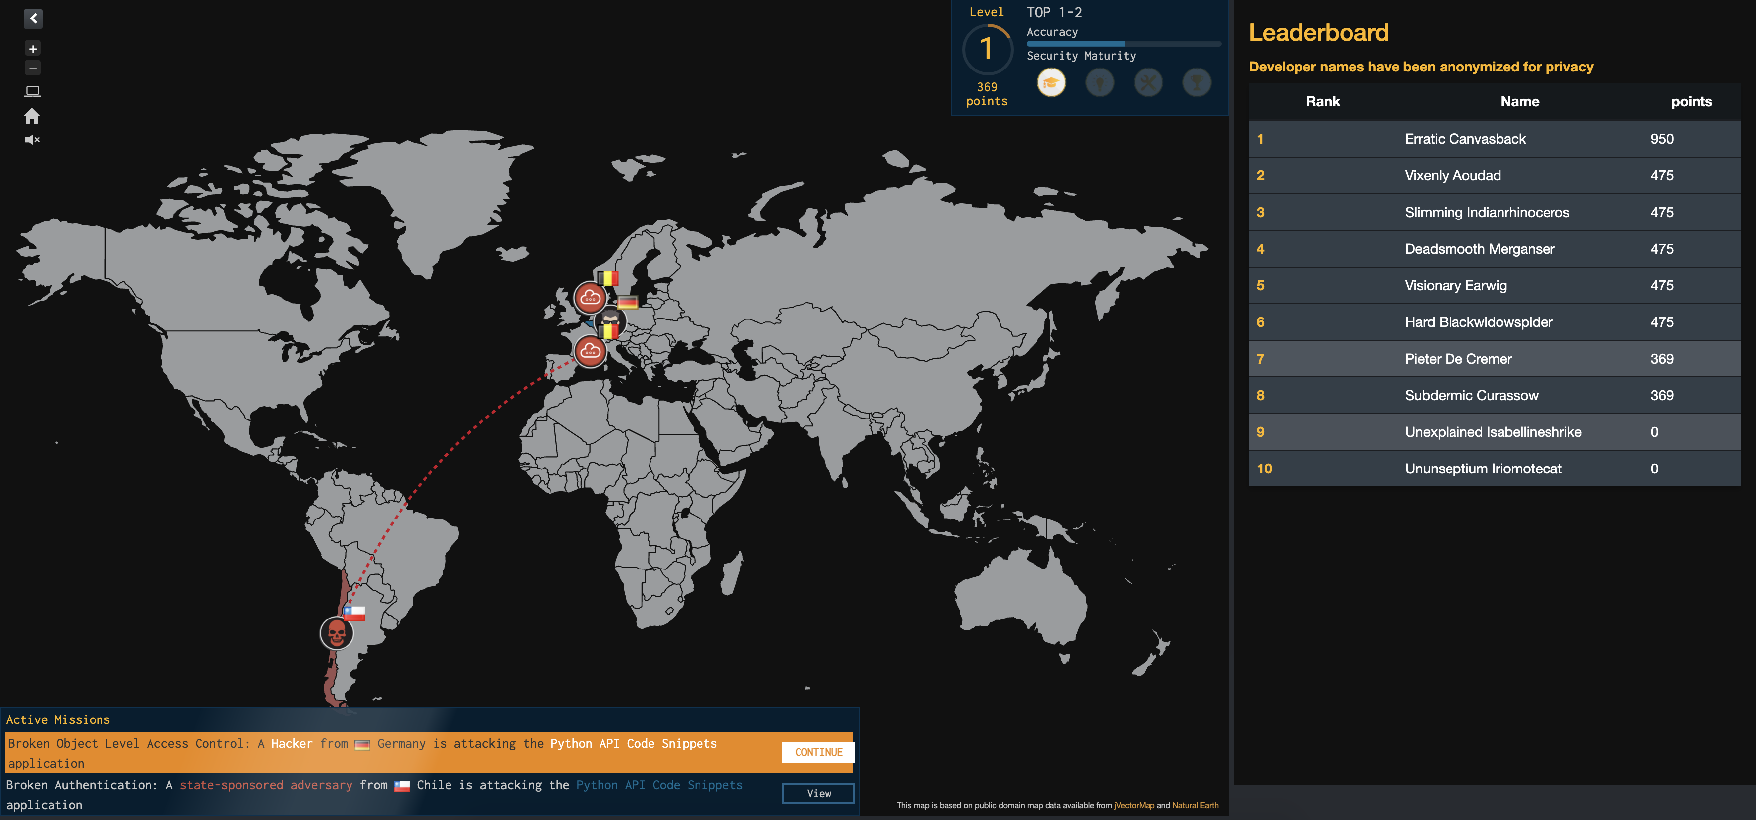
\includegraphics[width=\textwidth]{mission.pdf}
  \caption[SCW mission control dashboard]{The mission control dashboard on the \gls{scw} platform creates a gamified overview of the exercises.}
  \label{fig:mission} 
\end{sidewaysfigure}

\begin{sidewaysfigure}
  \centering
  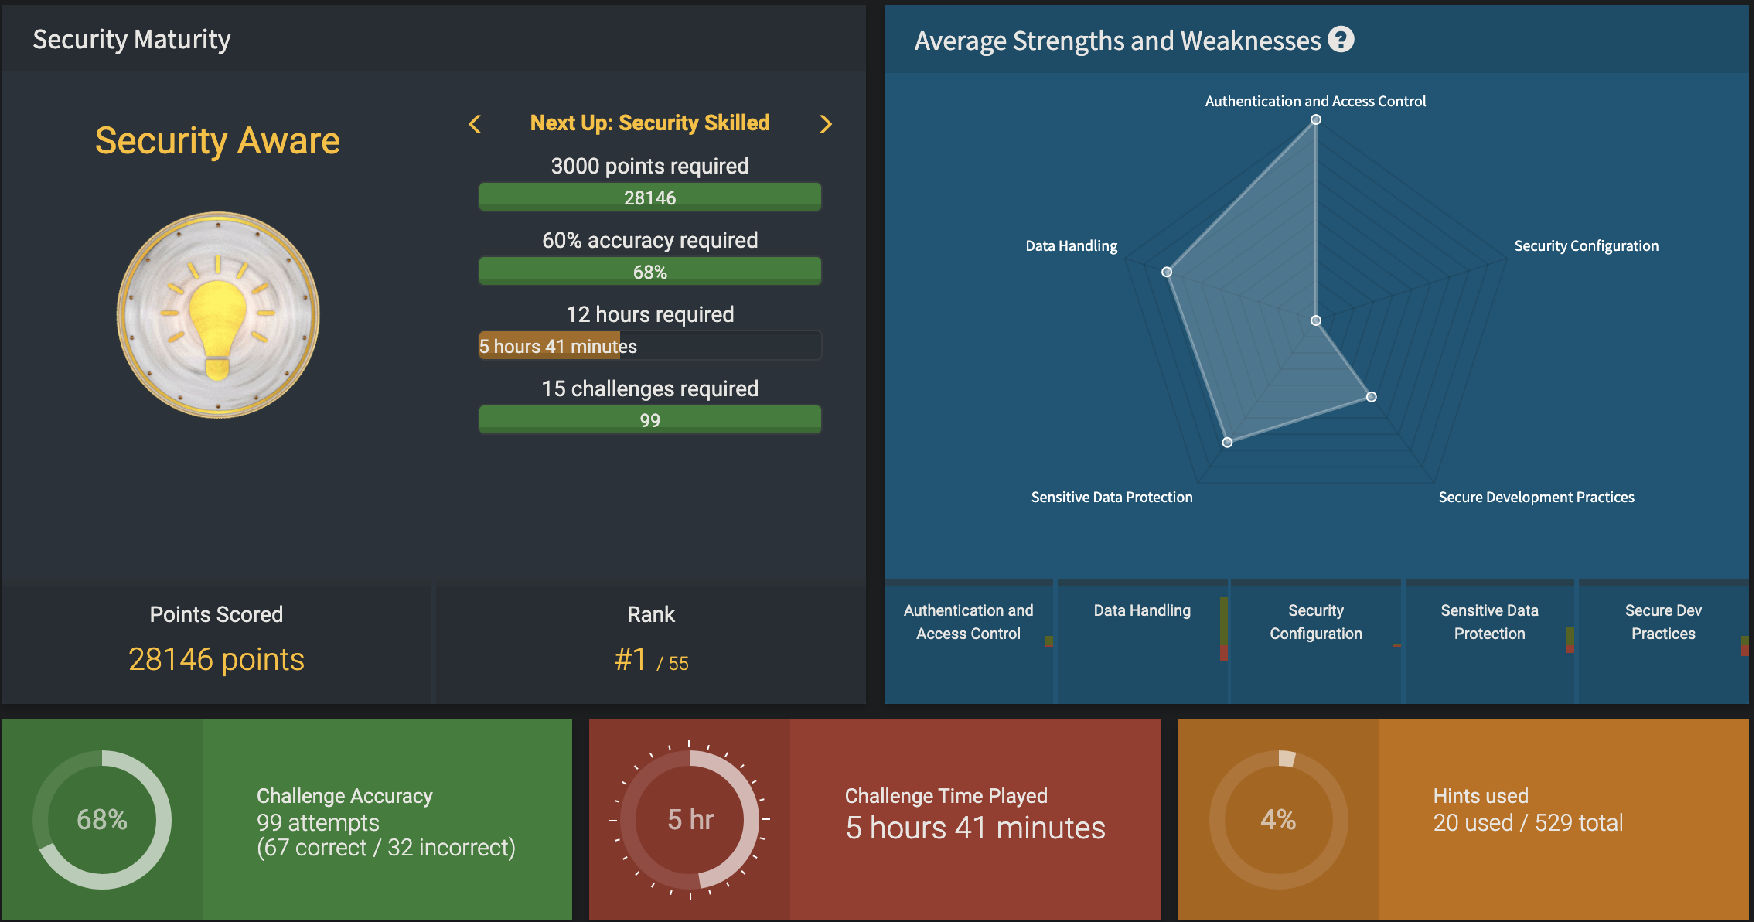
\includegraphics[width=\textwidth]{metrics.pdf}
  \caption[SCW metrics dashboard]{The metrics dashboard on the \gls{scw} platform allows developers to monitor their progress and unlock new badges.}
  \label{fig:metrics} 
\end{sidewaysfigure}

\section{Exercises}
\label{sec:challenges}
Training exercises on the \gls{scw} platform, often called challenges, are most frequently created from a complete and secure software application such as a webstore or a banking application. To create a challenge, a \gls{vulnerability} is introduced into this application on purpose.
The challenge is presented to the users as one of three types of exercises, each assigned a numerical level, an \textit{identify} (L1), \textit{locate} (L2), or \textit{fix} exercise (L3).

Identify exercises (L1) mark the insecure code fragment and provide the developer with a number of \gls{vulnerability} categories. It is up to the developer to identify which of the provided categories best describes the vulnerability present in the code fragment. In Figure~\ref{fig:identify} an identify exercise is shown based on a \gls{sql} injection in a Python web application.

For locate exercises (L2), the category of the vulnerability that is present in the insecure code fragment is given.
The insecure code fragment is marked, as well as several other (secure) code fragments. 
It is up to the developer to locate which code fragment contains the insecurity.
An example of a locate exercise is shown in Figure~\ref{fig:locate} using the same \gls{sql} injection in the same Python web application as the identify exercise in Figure~\ref{fig:identify}.

Fix exercises (L3) show both the insecure code fragment and the category of the inserted vulnerability to the user. 
Four alternatives are shown, with changes made to the insecure code fragment, and sometimes to other parts of the application code as well.
The developer needs to find the most secure alternative among the four options.
A fix exercise is shown in Figure~\ref{fig:fix}, again using the same \gls{sql} injection as before. 
Fix (L3) exercises are often combined with identify (L1) or locate (L2) exercises. 
These challenges then consist of two stages, in the first stage the vulnerability needs to be identified or located, in the second stage the exact same vulnerability needs to be fixed. 
The resulting two-stage challenge is an identify-and-fix (L4 = L1 + L3) or a locate-and-fix (L5 = L2 + L3) challenge.

%\begin{figure}
%\centering
%\begin{subfigure}[b]{\textwidth}
%\sidebysidecaption{0.05\linewidth}{0.95\linewidth}{
%   \caption{}
%   \label{fig:identify}}{
%   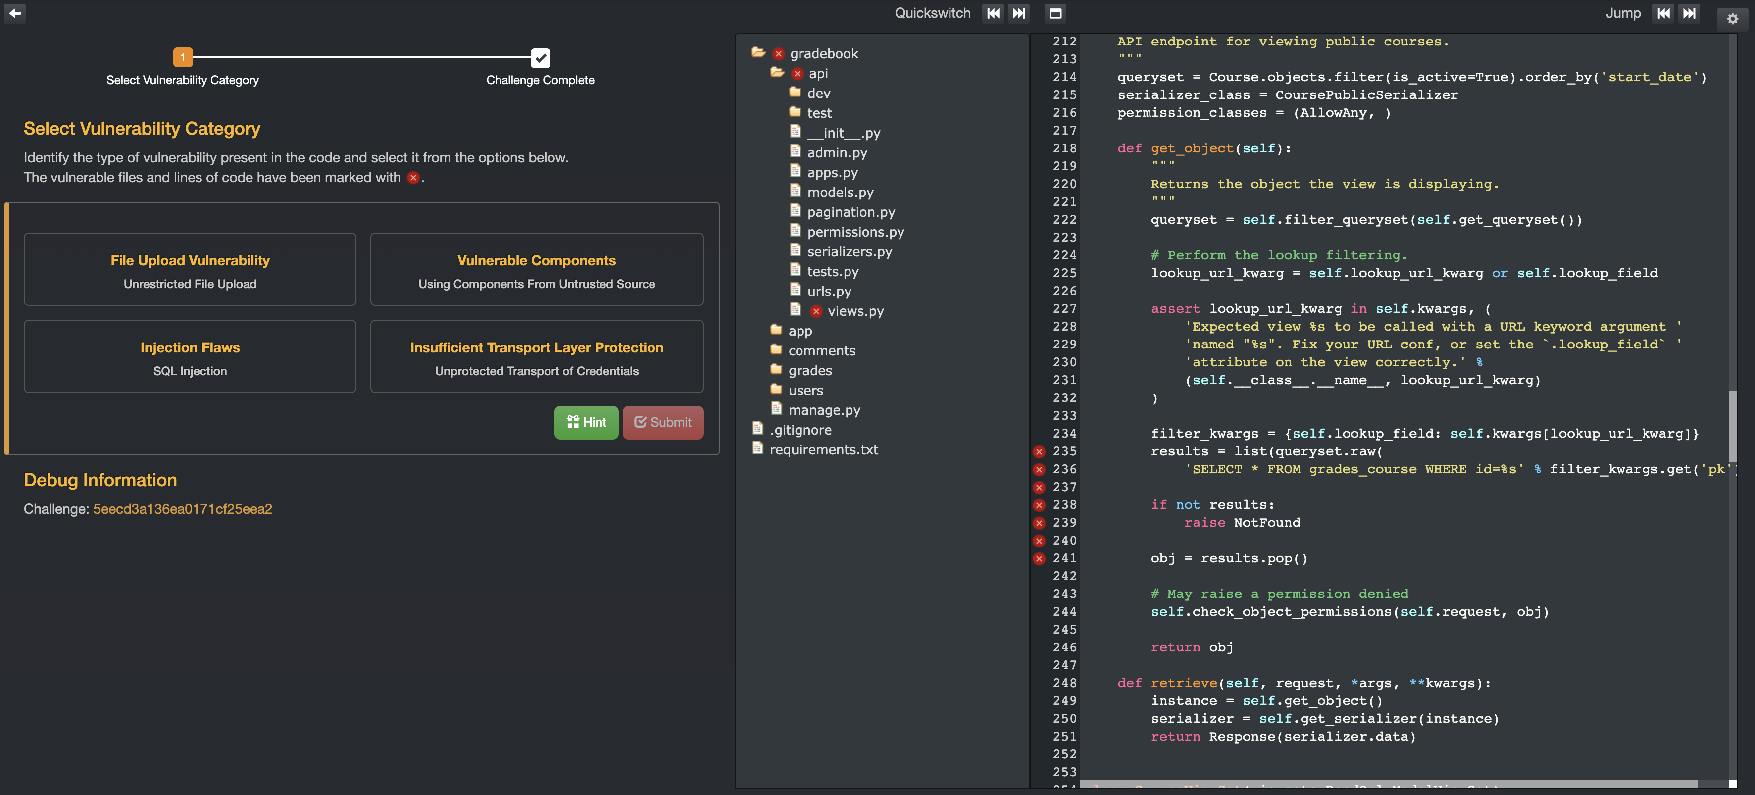
\includegraphics[width=0.95\linewidth]{identify.pdf}}
%\end{subfigure}
%
%\begin{subfigure}[b]{\textwidth}
%\sidebysidecaption{0.05\linewidth}{0.95\linewidth}{
%   \caption{}
%   \label{fig:locate}}{
%   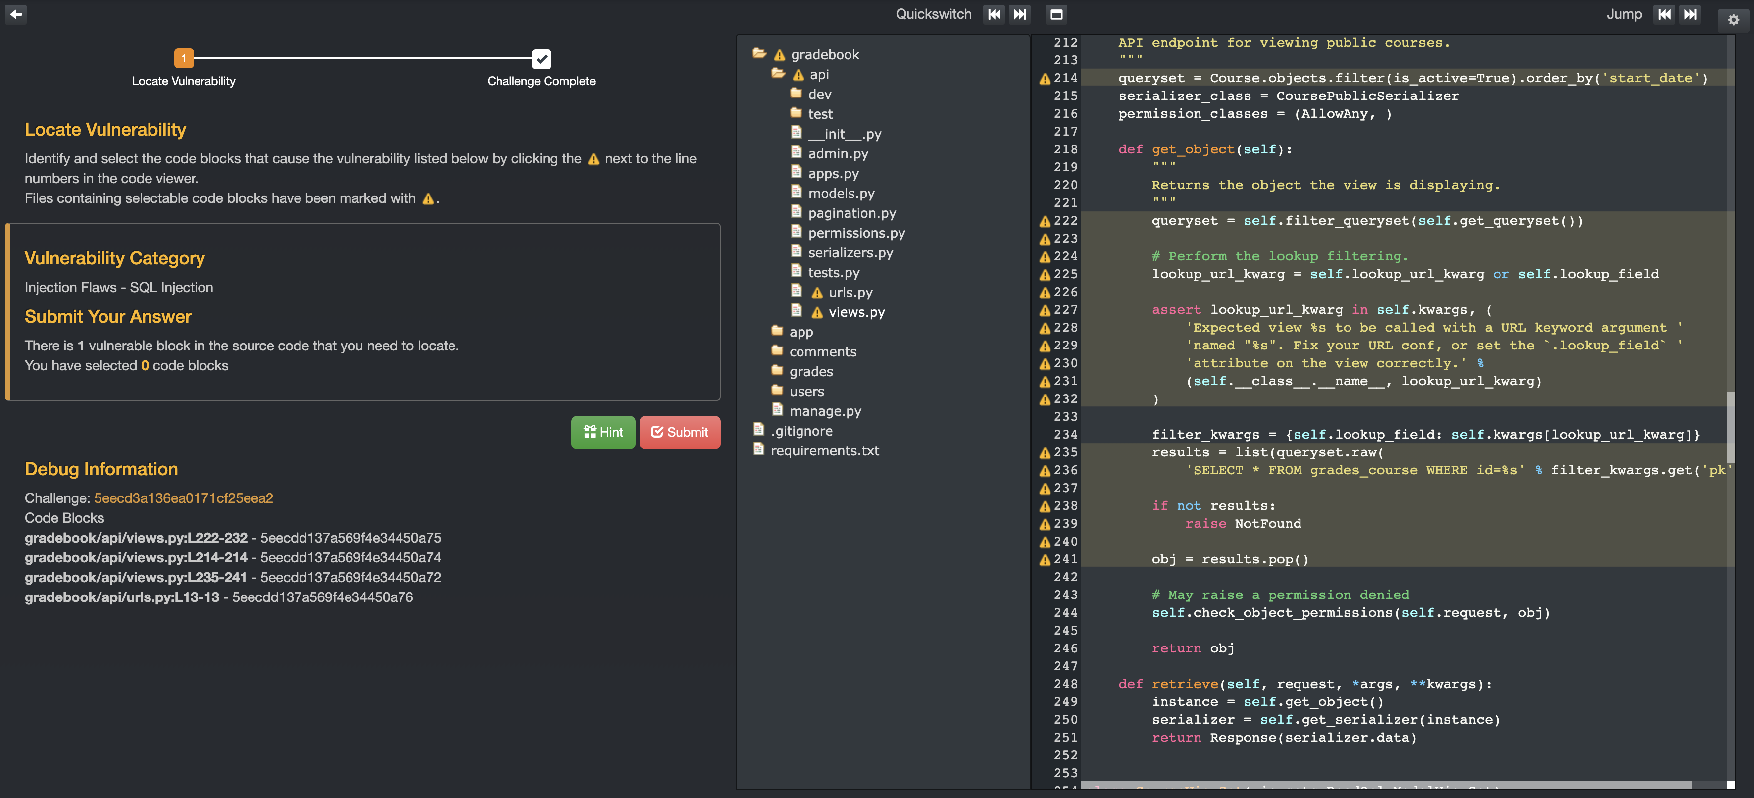
\includegraphics[width=0.95\linewidth]{locate.pdf}}
%\end{subfigure}
%
%\begin{subfigure}[b]{\textwidth}
%\sidebysidecaption{0.05\linewidth}{0.95\linewidth}{
%   \caption{}
%   \label{fig:fix}}{
%   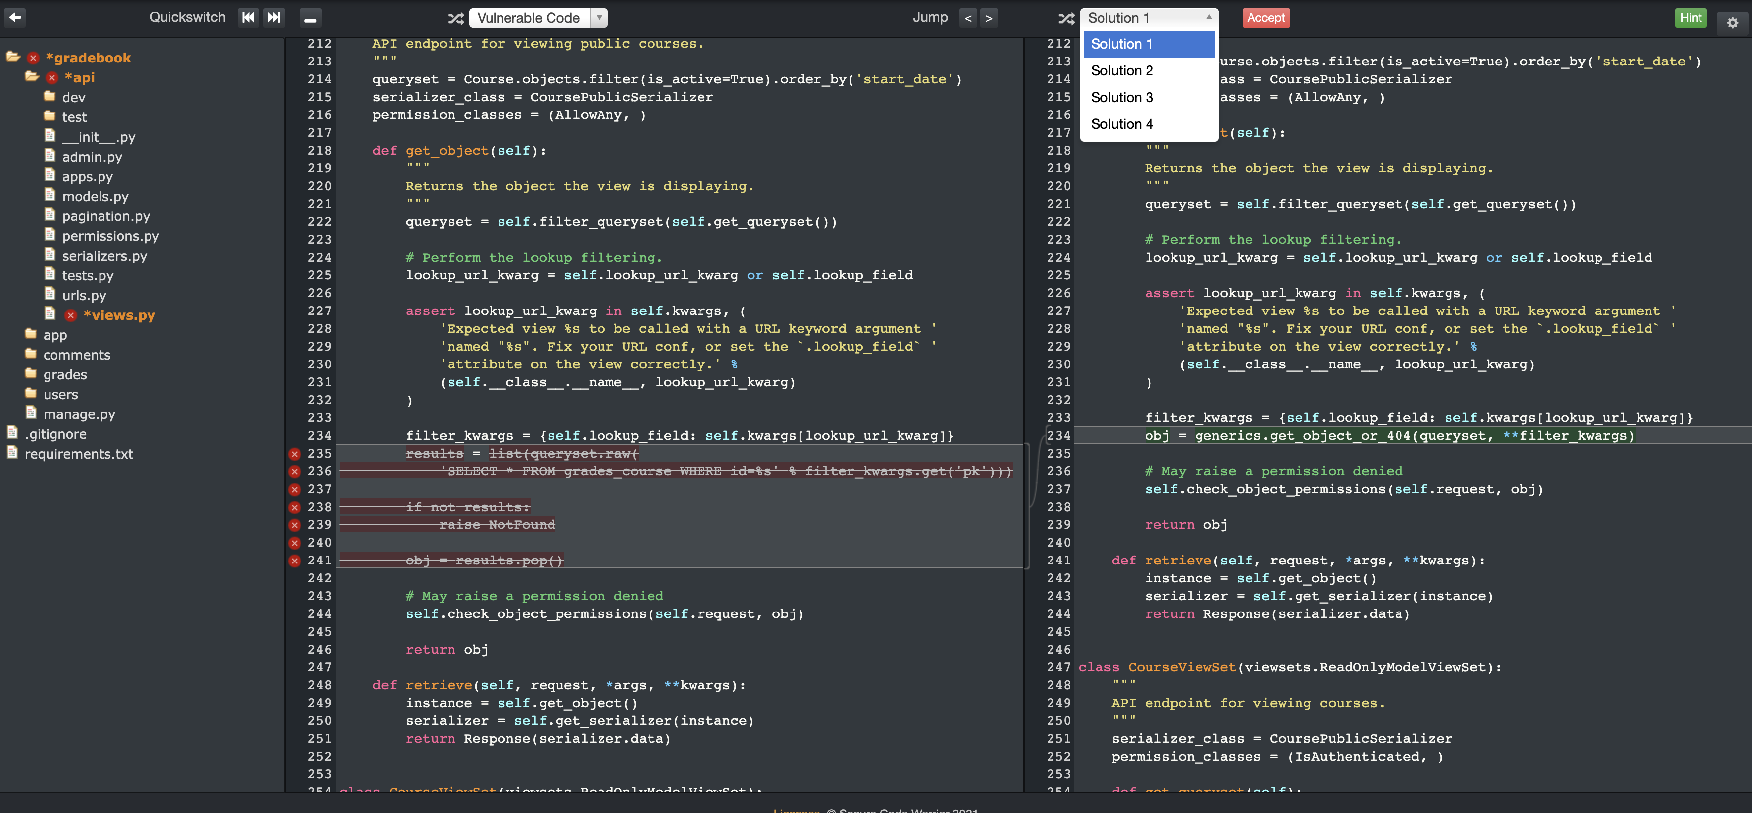
\includegraphics[width=0.95\linewidth]{fix.pdf}}
%\end{subfigure}
%
%\caption[Locate, identify, and fix challenges]{A single vulnerability in a software application can be presented to the developer as three different challenge types. \textit{Identify} exercises (a) mark the vulnerable code fragment and require the developer to select the right category. \textit{Locate} exercises (b) present the vulnerability category and require the developer to select the code fragment containing this vulnerability. \textit{Fix} exercises (c) require the developer to find the secure option among four alternative code bases.}
%\end{figure}

\begin{sidewaysfigure}
  \centering
  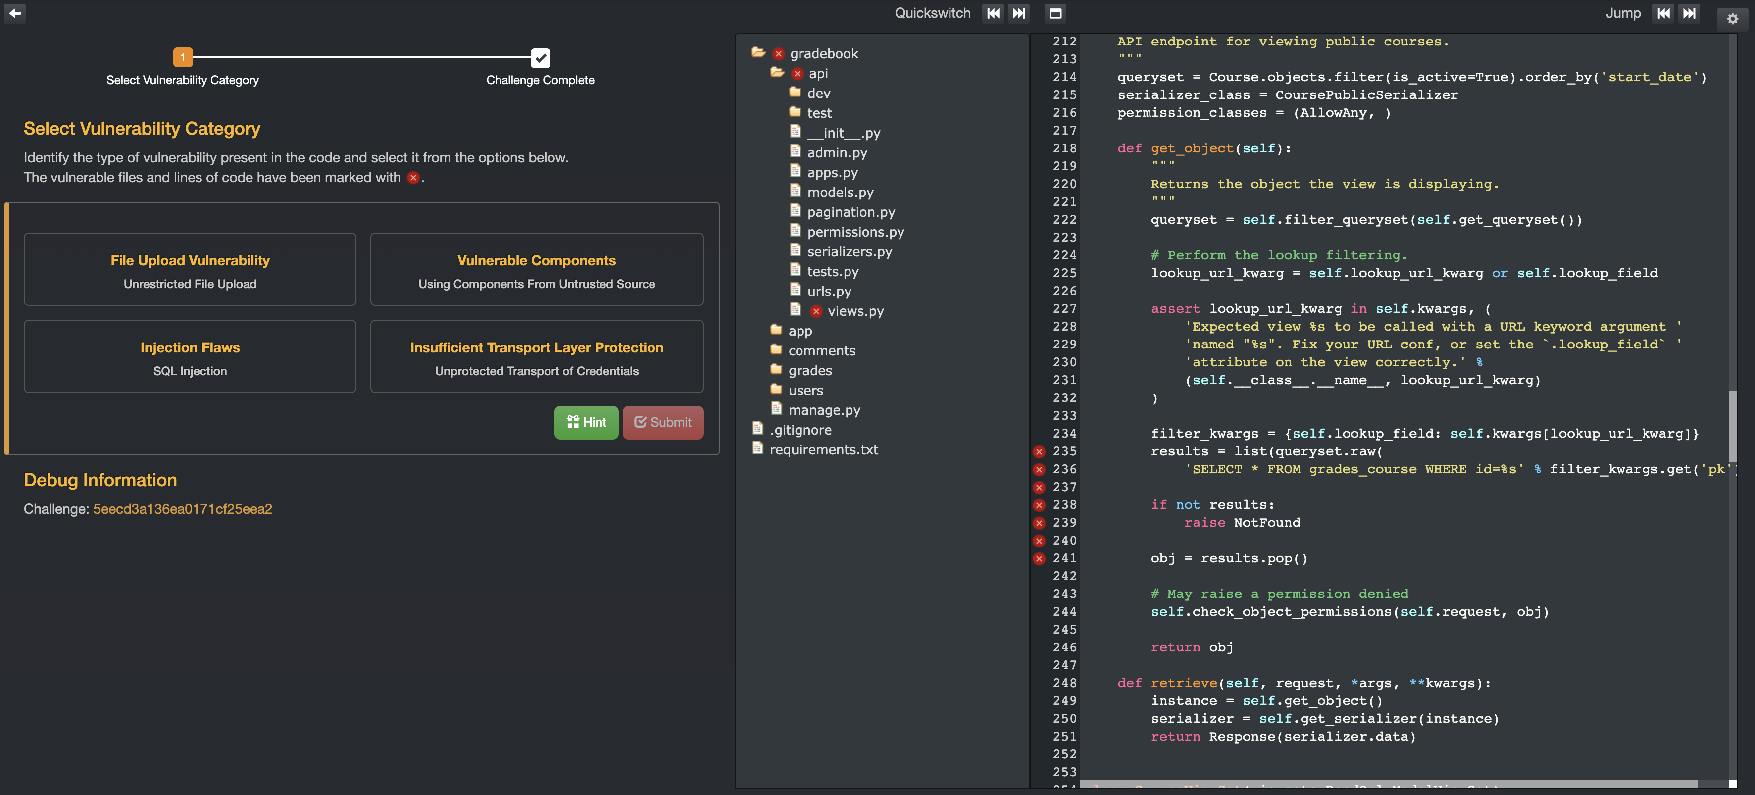
\includegraphics[width=\textwidth]{identify.pdf}
  \caption[Identify challenge]{\Gls{sql} injection in a Python web application presented as an identify exercise, the first of three different challenge types on the \gls{scw} platform.}
  \label{fig:identify} 
\end{sidewaysfigure}

\begin{sidewaysfigure}
  \centering
  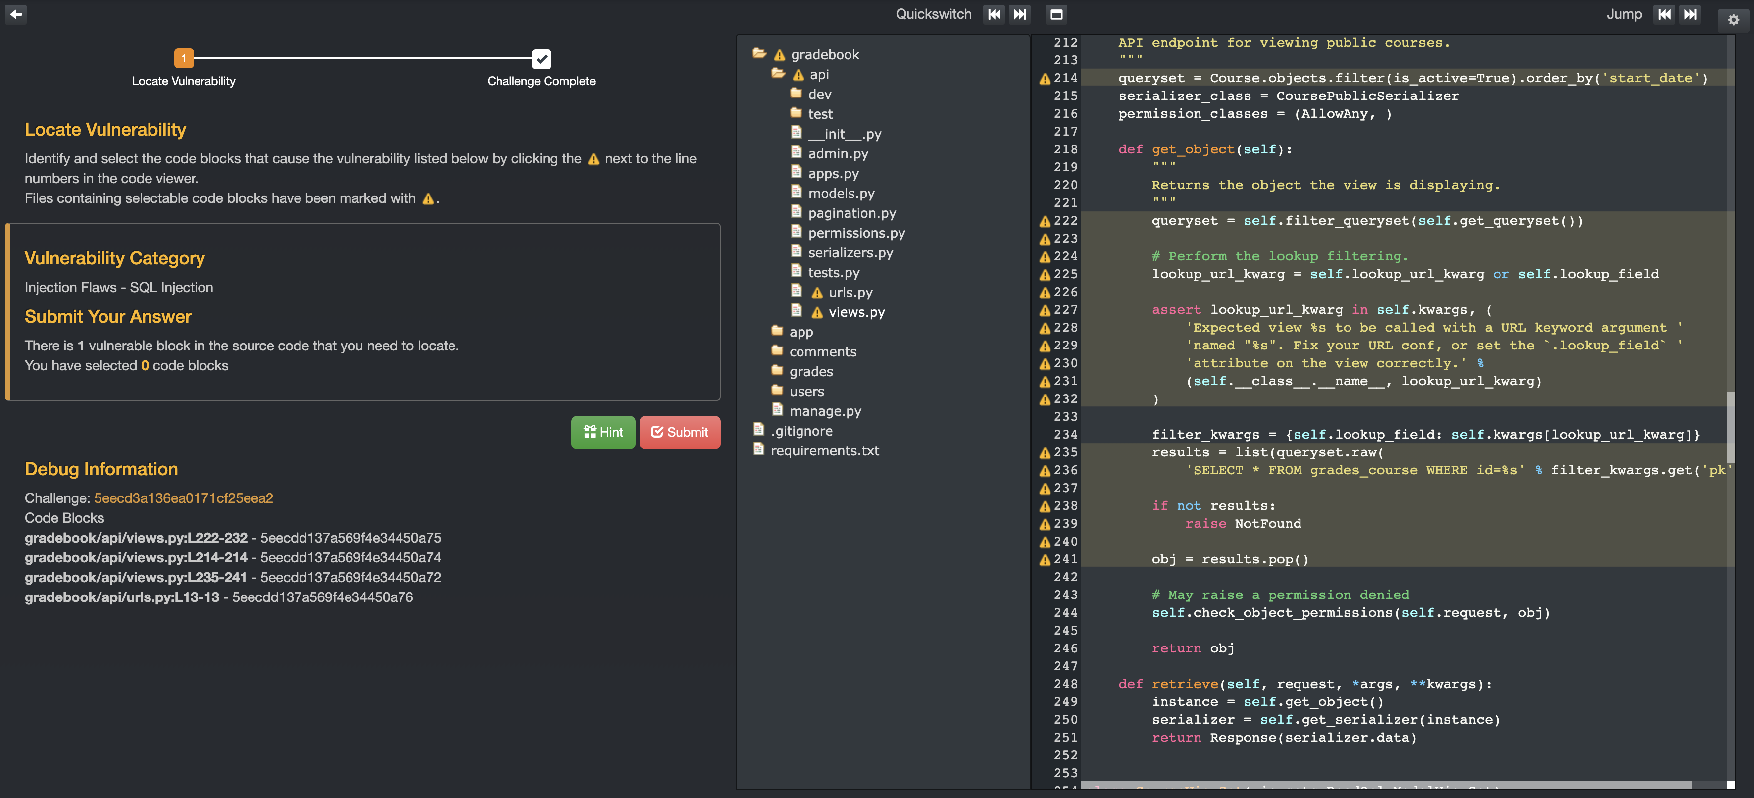
\includegraphics[width=\textwidth]{locate.pdf}
  \caption[Locate challenge]{\Gls{sql} injection in a Python web application presented as a locate exercise, the second of three different challenge types on the \gls{scw} platform.}
  \label{fig:locate} 
\end{sidewaysfigure}

\begin{sidewaysfigure}
  \centering
  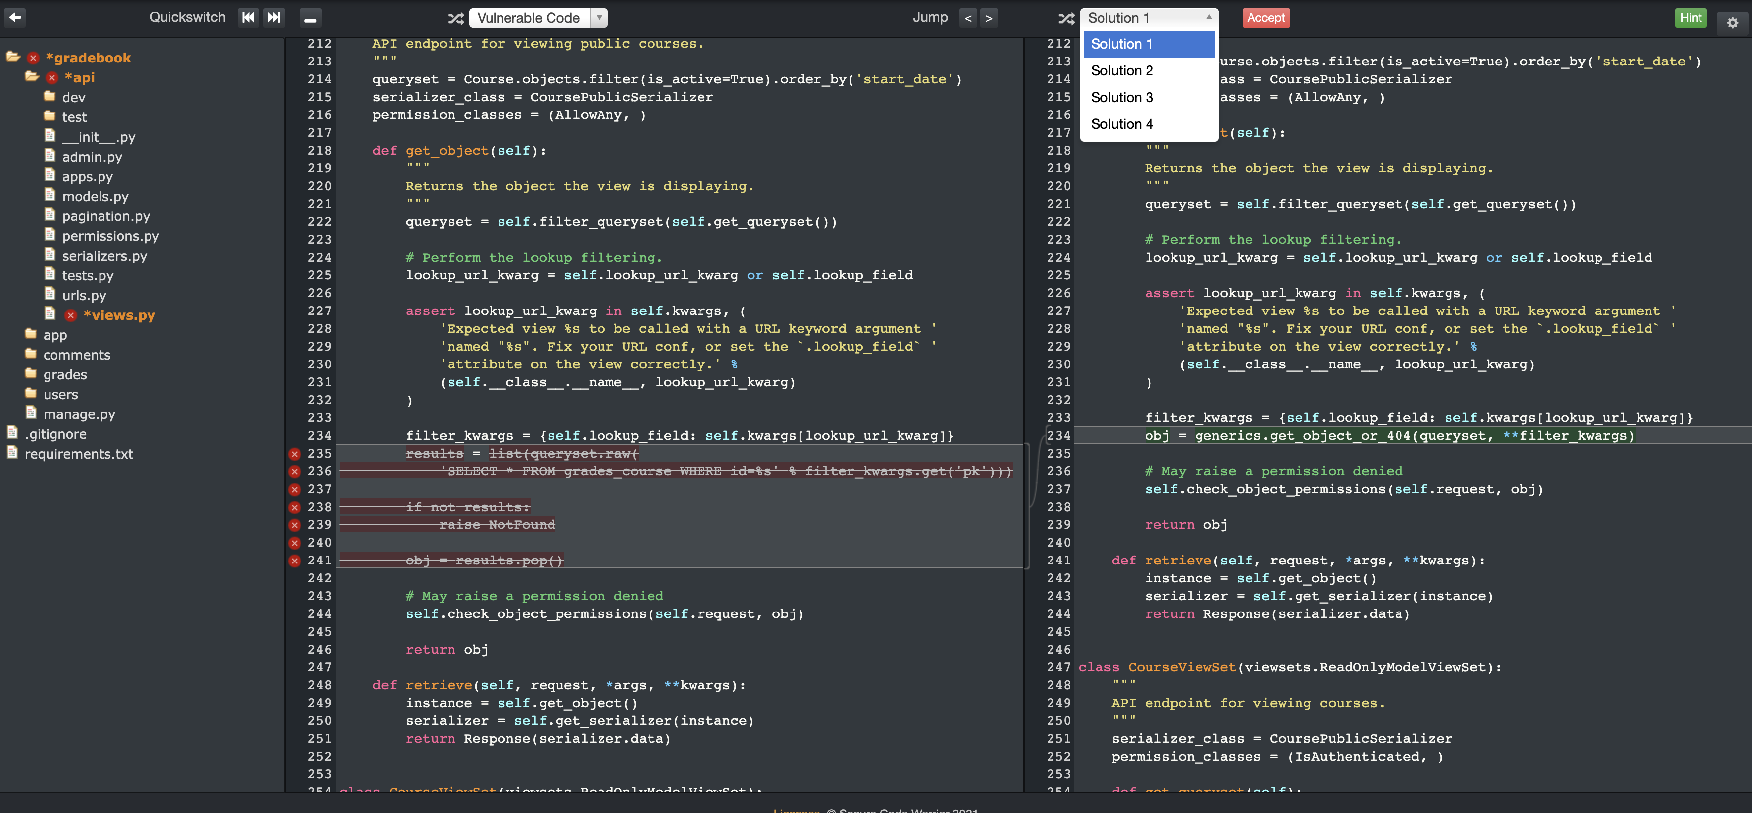
\includegraphics[width=\textwidth]{fix.pdf}
  \caption[Fix challenge]{\Gls{sql} injection in a Python web application presented as a fix exercise, the thrid of three different challenge types on the \gls{scw} platform.}
  \label{fig:fix} 
\end{sidewaysfigure}

Recently new and more interactive challenge types are being developed. 
One such type requires the developer to construct input that successfully exploits the vulnerability present in the application. 

\section{Context}
The challenges are presented to users in different contexts, these are training mode, tournament mode, or assessment mode.

The default context is the training mode.
In this mode the developer is allowed to use as many hints as needed.
They are also allowed an unlimited amount of attempts to find the right answer.
Each hint or failed attempt reduces the amount of points that the developer is awarded.
Appendix~\ref{app:challenges} describes in more detail how the difficulty of a challenge, the amount of hints used, and the number of failed attempts determine how many points are awarded. 
Developers are free to choose which challenges they solve first in training.
A standard course that guides them through the \gls{owasp} Top 10 categories is provided, and many developers complete this course before trying other challenges.

In tournament mode, the scoring method and availability of hints and attempts can be adjusted by the host.
In this mode, all participants are shown exercises about the same vulnerability type and of the same difficulty but in their language of choice.
The tournament is run for a limited time, usually a few hours, in which the contestants can complete the challenges.
In tournament mode, a live leaderboard is visible that can optionally be hidden close to the end for suspense.
Since all participants are shown the same number of exercises having the same difficulty, it often comes down to speed to finish the challenges in time, and accuracy to lose as few points as possible through hints or mistakes.

In assessment mode no hints are available and only one attempt is allowed for each challenge. This mode is used to evaluate the performance of a user.
Customers can select the vulnerability type and difficulty of the challenges making up the assessment.
There are some templates provided as an example that test for knowledge of the \gls{owasp} Top 10.

\section{Course material}
The \gls{scw} training portal provides training in more than 50 languages and frameworks\footnote{\url{https://www.securecodewarrior.com/supported-languages}}, ranging from Cobol to Go, including languages for web, mobile, cloud, and embedded software.
The training content covers 184 different vulnerability types, including those in widely-used lists such as the \gls{owasp} Top 10\footnote{\url{https://owasp.org/www-project-top-ten/}}, \gls{owasp} Top 10 Mobile, \gls{owasp} Top 10 \gls{api} Security and the \gls{cwe} Top 25\footnote{\url{https://cwe.mitre.org/top25}}.
The full list of vulnerabilities can be found on the \gls{scw} website\footnote{\url{https://www.securecodewarrior.com/product/supported-vulnerabilities}}.
This coverage is not homogeneous across all languages.
For each language and framework, each relevant vulnerability type is assigned a priority (high, medium, or low).
This priority depends on the severity and prevalence of the vulnerability type in this particular language and framework combination.

How well a language is covered then depends on the amount of challenges that covers vulnerability types of different priorities. 
The minimum requirement for a language to be considered ready for training is three challenges for each category in the \gls{owasp} Top 10 categories.
A language is considered tournament ready when there are five challenges (two easy, two medium and one high difficulty) for all vulnerability types with high priority, and two challenges (one easy, one medium) for all vulnerability types with medium priority.
There are other requirements still for assessments, specific courses, or the website trial.

For each of the top three frameworks over 450 unique vulnerabilities have been introduced in applications. These frameworks are C\# \gls{mvc} (461 vulnerabilities), Java \gls{ee} \gls{jsp} (475 vulnerabilities), and Java \gls{ee} Spring (495 vulnerabilities). When multiplied by three (for identify, locate, and fix), there are over 1350 challenges for each of these three frameworks.

\section{Use in the paved path methodology}
The \gls{scw} online learning platform is a great educational resource to support the paved path methodology.
The platform is \textit{relevant}, the learning context resembles the developer's work context as they are able to receive training in their office or home office and by looking at actual code. 
The code on the platform is likely to be similar to that of the developer due to the wide variety of programming languages, frameworks, and software types that are supported. 
The exercises teach a developer a secure paved path in their framework of choice. The identify, locate, and fix exercises are all defensive tasks created with the developer in mind.

The platform is also \textit{usable} as there are several features to increase interactivity and engagement, such as the gamified theme, leaderboards, tournaments, achievements, and badges.
A structured journey is present in the form of courses, such as the \gls{owasp} Top 10 courses.
The learning material is presented through multiple choice questions.
In newly released exercise, developers are even be allowed to discover the answer through trial and error instead of picking from a list of options.

% the NEED
There is certainly enough content available to allow for sufficient repetition so that the concepts can be committed to memory, with some frameworks providing as many as 1350 challenges.
However, there is no guidance to find the right balance between repetition and \textit{efficiency}.
The exercises often do not match the learning pace of each individual, leading to boredom or frustration.
This is apparent from the challenge completion rate, as only 45\% of users complete more than 30 challenges, the amount of challenges in an \gls{owasp} top 10 course.

When surveyed, some users indicate this possible mismatch in the learning pace.
More than 700 respondents were asked to describe their experience using the \gls{scw} portal after completing a tournament.
To do this, they were able to choose words from a set of options or write their own.
Many respondents selected words indicating their engagement such as interactive (55\%), engaging (53\%), and fun (48\%).
But some also picked words that could indicate an incorrect learning pace, among which challenging (45\%), repetitive (21\%), long (7\%), and boring (4\%).
Only 22 (3\%) respondents wrote down additional words themselves, some of which indicate mismatches in learning pace. 
Two users wrote down tedious, two users wrote cumbersome, one wrote frustrating, and one even went as far as to describe their experience as gambling.

In conclusion, the \gls{scw} online learning platform is a good educational resource when using a paved path methodology. Its defensive exercises and wide support for different programming languages and frameworks make it \textit{relevant} to the developer's work. The gamification and interactivity keep it \textit{usable} and fun. However, when it comes to the \textit{efficiency} of the training, there is still room for improvement, as currently all users are presented with challenges of the same difficulty regardless of their skill level and learning pace.
User feedback indicates that this leads to boredom or frustration for some of the users. 
\chapter{Intelligent tutoring system}
\label{ch:its-implementation}
\glsreset{its}
%(CONTEXT): background for less specialized readers and establish or recalls the importance of the problem
An important aspect of education in the paved path methodology is its efficiency.
Educational activities should not keep the developer from their responsibilities for longer than necessary.
% (NEED): motivates the audience by stating the difference between the desired and actual situation
% ==>shortcomings and goal from my perspective
The efficiency of training on the \gls{scw} platform is lacking.
Because every individual is presented with the same exercises, they often receive training that is too repetitive or too challenging.
%(The TASK) what did I do?
%=> IRT, ITS
I designed an \gls{its} that recommends exercises to each individual at any point in time to provide them with a more appropriate learning pace.
%When evaluating online learning activities, the focus is often wrongfully on completion and dropout rates~\cite{hadi2016driving}. 
%It is perfectly possible, likely even, that learning took place despite the user not completing the course.
%The goal of the \gls{its} should hence be to maximize the opportunity for learning to take place.
% OBJECT
In this chapter, I present the design of the \gls{its} and discuss the used techniques in its implementation in more detail.
%In this chapter we start with an overview of the design of the \gls{its} in Section~\ref{sec:design}.
%In the rest of the chapter we explain the used techniques in more detail.
%First, the collaborative filtering algorithm is detailed in Section~\ref{sec:collab}.
%Next, the psychometric models are discussed in Section~\ref{sec:calib}.

\summarybox{
I designed an \gls{its} that consists of three algorithmic components, one for exercise selection, and one each for estimation of user ability and exercise difficulty.
Exercise selection is achieved through a \gls{cf} algorithm adapted to learning systems.
In such an algorithm, a target user's preference for an exercise is predicted based on the preferences of like-minded users.
Through the use of the psychometric model of \gls{irt}, estimation of both user ability and exercise difficulty can be done at once.
A sanitized data set of over 9 million solved exercises is used to calibrate these algorithms making up the \gls{its}.
}

% SECTIONS
\section{Design}
\label{sec:design}
The design of the \gls{its} shown in Figure~\ref{fig:its-overview} extends the existing functionality of the training platform.
This existing functionality is depicted in orange on the right side of the figure, while components of the \gls{its} are drawn in blue on the left side.
The \gls{its} consists of two loops, it contains three algorithmic components and three types of data collections.

% high level overview of different components of ITS
\begin{figure}
    \centering
    %\input{03-education/plots/its-flowchart-reverse}
    \includegraphics[page=12]{03-education/figures/tikzfigures.pdf}
  \caption[Design of the ITS]{The \Gls{its} consists of two loops. In the main loop, users are served exercises and their answers are processed, before selecting a new exercise. The user history is then regularly used in a secondary loop to estimate both user abilities and exercise difficulties.}
  \label{fig:its-overview} 
\end{figure}

The algorithmic component in the main loop is that of exercise selection.
Selecting the optimal exercise is done through an adapted \gls{cf} algorithm, as will be explained in more detail in Section~\ref{sec:collab}.
In this technique, a recommendation is derived from historical data of like-minded users.
To evaluate this technique, and hence improve it, we need a measure to decide what a good recommendation is.

A useful challenge is a challenge from which the user has learned something and that keeps the user engaged.
That is, a good recommendation system should increase the \textit{ability} of the user, and their \textit{engagement}.
It is easy to keep track of the engagement of the user.
If they continue to play more challenges, that means they stay engaged.
However, in order to determine if a recommendation leads to increased ability, we need to be able to continuously measure the ability of each user.
Another reason to continuously measure the ability of each user is the temporal aspect to learning.
An exercise that is useful to a user at the beginning of their journey is likely no longer an appropriate recommendation once their ability has sufficiently increased.
Hence ability estimation is needed to both determine \textit{if} a challenge was useful to a user, and \textit{when} a challenge was useful.

A very naive way to achieve an ability estimate is simply looking at the accuracy of each user.
A user answering all of the challenges correctly (100\% accuracy), is likely to have a higher ability level than a user answering half of them correctly (50\% accuracy).
If all users completed the exact same challenges, this could give a reasonably accurate representation of their ability level.
In fact, that is exactly the reasoning behind \gls{ctt}~\cite{ctt}.
In a classic test all examinees are given the same (or equivalent) exercises and their accuracy on the test is an indication of their ability level.

However, on the training platform not all users are completing the exact same challenges and this is not desirable, as that would conflict with the goal of individually tailored recommendations.
When users are completing different challenges, accuracy alone is no longer sufficient.
It is possible for one user to maintain a high accuracy doing simple challenges, while another user's accuracy is lower but they are completing difficult challenges.

This is also true for exercises, the difficulty of an exercise can not be accurately estimated through the accuracy of users completing it.
It is possible for one exercise to have a high accuracy because it is mostly attempted by users of a high ability level, while another is often tried by beginners and hence has a lower accuracy.
It is clear that these two remaining algorithmic components in the \gls{its} are tightly coupled.
Both are implemented through the use of psychometric models from the field of \gls{irt} as explained in Section~\ref{sec:calib}.
The calibration techniques of \gls{irt} use the entire user history and take a while to complete.
This is why they are not performed every iteration of the main loop, but at regular intervals in a secondary loop.

\section{Collaborative filtering}
\label{sec:collab}

In this section, I discuss the first algorithmic component of the \gls{its} as depicted in Figure~\ref{fig:its-overview}, the component of exercise selection.

There are many possible factors that determine which exercise to select.
We can easily imagine some factors that are likely to have a big influence, such as the difficulty of the exercise, the vulnerability type, and the programming language.
Research has also shown that individual learning style has an impact on learning performance~\cite{alshammari2015design,schiaffino2008eteacher,graf2006representative,felder1988learning}.
For other factors, it is more difficult to determine how important they are, or if they matter at all.
Some examples are code quality, code legibility, software type, or even just the coding style of the author of the challenge.
There are also likely other factors that we are not yet aware of.

For this reason, it is desirable to create a recommendation system that uses a black box approach.
With this kind of approach it is not necessary to know which factors determine a good recommendation.
There only need to be enough users and challenges, as well as a way to determine if a challenge was useful to a user.

One frequently used technique for recommendation systems is \gls{cf}.
In \gls{cf}, a target user's affinity for items is used to find other users who are most like-minded.
This group's collective affinity for items is then used to predict the target user's affinity for those items.

These types of algorithms are most easily understood through a visual representation. 
In Figure~\ref{fig:cf}, a simple example of a \gls{cf} algorithm is illustrated.
In this figure, the recorded affinity of users $i$ $(i = 0,\dots,5)$ for movies $j$ $(j = A,\dots,J)$ is depicted in a two dimensional grid.
A green check mark in the grid means that the user enjoyed the movie, a red cross means they did not.
There are also many empty spaces as not all users have watched all movies.
In order to predict the affinity of a target user $i = 0$ for a target movie $j = B$, the \gls{cf} algorithm starts by finding the users who are most like-minded, the users who have the most similar recorded affinity.
For each user, the algorithm determines for how many movies they have the same affinity as the target user.
In Figure~\ref{fig:cf}, the affinity of the target user is marked with an orange background, affinity of other users that is the same as the target user is marked with a green background.
In the example, user $i = 1$ enjoyed movies $j \in \{A,C\}$.
But their affinity for movie $C$ is the only affinity they have in common with the target user.
Users $i \in \{2,3,5\}$ each have the same affinity as the target user for two of the movies. 
In this example, they make up the group of people that are most like-minded to the target user.
To predict if the target user would enjoy the target movie $j = B$, the algorithm now uses this group's affinity for the target movie, marked in a blue background in Figure~\ref{fig:cf}.
Two of the most like-minded users enjoyed the movie and one of them did not.
Since the majority of like-minded users enjoy the target movie, the algorithm predicts the target user might enjoy it as well.

\begin{figure}
    \centering
    %\input{03-education/plots/collaborative-filtering}
    \includegraphics[page=7,width=\textwidth]{03-education/figures/tikzfigures.pdf}
    \caption[Collaborative filtering algorithm]{Visual representation of the steps to determine if the target movie $j=B$ is a good recommendation for the target user $i=0$. 
    The \gls{cf} algorithm first finds all users who have similar preferences for movies as the target user (marked in green). 
    The users who have the most similar preferences are used in a majority vote. 
    In the example users 2, 3, and 5 each had the same preference as the target user for two different movies.
    The majority of these users enjoyed the target movie (marked in blue), so the algorithm concludes that the target is a good recommendation.}
    \label{fig:cf}
\end{figure}

\subsection{Adapted to learning systems}
\label{sec:adapted-cf}
Some adjustments are needed to apply \gls{cf} to a learning system.
In a learning system, a good recommendation is one that allows meaningful learning to take place and at the same time keeps the user engaged.
A good recommendation is hence based on the \textit{utility} of a user for an item, rather than their affinity.
If the users who are most like-minded increased their ability level through playing this challenge, it is likely a good recommendation.

As mentioned before, learning also has a more apparent temporal aspect to it.
An exercise that is useful to a user at the start is no longer an appropriate recommendation once their ability has increased sufficiently.
It could hence be beneficial to keep track of the ability level around which a recommendation can be deemed appropriate.
The \gls{cf} algorithm can then only consider users to be like-minded, if they experienced the same utility as the target user within a certain ability range.
Users who experienced the same utility for an item but at a sufficiently dissimilar ability level will not be considered like-minded users.

Figure~\ref{fig:3d-cf} illustrates how this adaptation could be achieved on the example algorithm from before.
In this figure, the recorded utility that the users $i$ $(i = 0,\dots,5)$ experienced from challenges $j$ $(j = A,\dots,J)$ is depicted in a two dimensional grid for three sufficiently distinct ability levels $\bm\theta$.
A green check mark means that this challenge was useful to the user around that ability level.
A red cross means it was not useful, and the user either did not learn anything, or the challenge caused the user to disengage from the training.
How the utility of a challenge is determined will be explained in Section~\ref{sec:utility}.
To predict the utility of the target challenge $j = B$ to the target user $i = 0$, the adapted \gls{cf} algorithm looks for the most like-minded users, the users who experienced the most similar utility.

However, only if the same utility was experienced around the same ability level does it count towards like-mindedness.
In Figure~\ref{fig:3d-cf}, utility that was experienced by the target user for challenges is marked with an orange background.
Similar utility that was experienced around the same ability level is marked with a green background.
At the lowest ability level, user $i = 2$ experienced the same utility as the target user for four challenges.
User $i = 1$, just like the target user, experienced challenge $j = C$ as useful.
However, the challenge was useful to user $i = 1$ at the lowest ability level, while the target user found this challenge useful when their ability level was sufficiently higher.
Similar utility like this that was experienced around a different ability level is marked with a red background in the figure.
This utility does not count towards like-mindedness.
Using this metric for like-mindedness, we find that users $i \in \{2,3,5\}$ each experienced the same utility around the same ability level as the target user for four different challenges.
They make up the group of users who are most like-minded to the target user.

Beyond this adaptation, the same steps are used to decide the final recommendation.
The majority of like-minded users experienced the target challenge as useful around the targeted ability level, marked with a blue background.
The algorithm concludes that the target challenge is a good recommendation for the target user.

\begin{figure}
    \centering
    %\input{03-education/plots/3d-collaborative-filtering}
    \includegraphics[width=\textwidth,page=3]{03-education/figures/tikzfigures.pdf}
    \caption[Adapted collaborative filtering algorithm]{Visual representation of the steps to determine if the target challenge $j=B$ is a good recommendation for the target user $i=0$. 
    The collaborative filtering algorithm first finds all users who experienced similar utility from challenges as the target user around the same ability level $\bm\theta$ (marked in green). 
    Similar utility at a different ability level is disregarded (marked in red).
    The users who experienced the most similar utility are used in a majority vote. 
    In the example, users 2, 3, and 5 each experienced the same utility as the target user for four different challenges.
    The majority of these users experienced the target challenge as useful (marked in blue), so the algorithm concludes that the target is a good recommendation.}
    \label{fig:3d-cf}
\end{figure}

\subsection{Types of collaborative filtering}
In the examples until now, the affinity (or utility) of a user for an item was considered binary, the user either liked it, or they did not.
In reality, often a more complex scale is used.
For example, Netflix movie recommendations use a rating scale between 1 and 5.
In this context, the affinity of a user $u$ for an item $i$ is often called the rating $r_{ui}$.
The goal of a \gls{cf} algorithm is then to make a prediction for this rating $\hat{r}_{ui}$.
\Gls{cf} algorithms can be split into two broad categories, memory-based and model-based algorithms, based on how they set out to achieve this goal~\cite{li2021novel,sharma2017collaborative,yu2004probabilistic,breese2013empirical,su2009survey}.

\subsubsection{Memory-based}
Memory-based \gls{cf} algorithms directly use observed ratings to compute predictions.
Generally, these algorithms mark a subset of users as neighbours to the target user by calculating the similarity between users~\cite{li2021novel,Hug2020}.
They then use the neighbour's ratings to predict the rating of the target user~\cite{su2009survey,Hug2020,Koren2010,Ricci2010}.

Memory-based \gls{cf} algorithms are frequently used in recommender systems and even commercial systems such as the Amazon webstore~\cite{sharma2017collaborative,yu2004probabilistic}.
The main advantages of memory-based collaborative filtering algorithms are that they are easy to implement, and that new data can be added easily and incrementally.
Their biggest shortcoming is a decreased performance for sparse data, when it is difficult to find sufficient neighbours.
They also can not make recommendations for new users or items as there is no data to do similarity computations with.
In the \gls{its} however, we already need sufficient data to compute the difficulty and ability estimates.
In a learning system, the need for an initial calibration phase can not be avoided, so this shortcoming does not impact the design of the \gls{its}.

Five different memory-based \gls{cf} algorithms are considered in this work. 
They will be described in more detail in the experiments in Section~\ref{sec:eval-cf}.
Four of these algorithms are \gls{knn} algorithms, they first determine the k nearest neighbours and then use the ratings of these neighbours to compute a prediction.
Because these algorithms use an explicit definition of similarity between users, they can be easily adapted to learning systems by changing this definition to take into account the ability of the users.
The remaining memory-based algorithm uses the ratings of all users to make a prediction, adapting it to learning systems will be harder, but can still be achieved by processing the data, as will be explained in the description of the experiments.

\subsubsection{Model-based}
Model-based \gls{cf} algorithms use statistical and machine learning methods to construct a model, and use this model to make predictions~\cite{sharma2017collaborative, li2021novel,sarwar2002recommender,heckerman2000dependency}.
These models often use techniques to reduce the dimensions of the matrix of user-item ratings.
This reduces the scalability and sparsity problems that are experienced by memory-based algorithms~\cite{sarwar2002recommender,moreno2016web}.
Model-based algorithms are often more accurate, but the construction of the model is often slow and expensive, and they have to be re-built regularly, every time new data is being added incrementally.

Algorithms using clustering techniques are simple examples of model-based algorithms~\cite{su2009survey,breese2013empirical,sarwar2002recommender,o1999clustering}.
Users or items are assigned to one or more clusters so that the matrix of user-item ratings becomes a smaller, denser matrix of clusters.
It is then possible to use statistics from these clusters to make predictions, for example, by taking the average rating of a cluster.
In the experiments of this work, one clustering algorithm is evaluated.

Thanks to their accuracy and scalability, model-based algorithms based on matrix factorization have gained a lot in popularity~\cite{Ricci2010}.
These algorithms use the technique of \gls{svd} to make a low rank approximation of the original ratings matrix~\cite{george2005scalable, Ricci2010, Hug2020}.
\Gls{svd} is a well-established technique in linear algebra and machine learning to identify latent semantic factors.
Applying it in the \gls{cf} domain raises a few difficulties due to the sparsity of the rating matrix, which increases the risk of overfitting.

In the experiments of this work, I evaluated \gls{pmf}~\cite{mnih2008probabilistic}, \gls{nnmf}~\cite{wang2012nonnegative,hoyer2004non}, \gls{svd}~\cite{sarwar2000application,polat2005svd,Ricci2010}, and \gls{svd}++~\cite{koren2008factorization,Ricci2010}.
All of these algorithms are explained in more detail in Section~\ref{sec:eval-cf}.

\subsection{Alternative approaches}
\label{sec:cf-alternatives}
Many existing alternatives either do not take into account the ability level of the users to make recommendations, or they only take into account the ability level~\cite{chen2005personalized}.

\subsubsection{Adaptive learning systems}
Many computerized learning systems already exist, both in commercial offerings and in research literature.
Older systems do not consider individual learners needs, but make decisions based on pre-planned instructions for the field of study.
As a result, these systems do not provide individual attention to students as a natural (human) teacher would~\cite{mahdi2016intelligent}.
This inspired the rise of more advanced learning systems that consider both the field and the learner to provide flexibility in the presentation of the educational material.
Some such systems have been built to teach computer science concepts, such as debugging~\cite{carter2013tutoring}, cryptographic algorithms~\cite{abuel2018intelligent,mahdi2016intelligent}, programming in C++~\cite{abu2009evaluating}, or \gls{sql}~\cite{mitrovic2003intelligent}.

These systems have varying degrees of intelligence and adaptiveness.
In commercial offerings, such as Pluralsight Iris\footnote{\url{https://www.pluralsight.com/product/iris}}, adaptive learning often refers to an initial calibration phase to determine the initial ability level of a user.
In other systems, students are allowed to advance to more difficult levels when a sufficiently high accuracy is achieved on exercises in the current level~\cite{abu2009evaluating,mahdi2016intelligent}.
Even more advanced systems provide adaptive feedback to the users, based on which mistakes have been made in the exercises~\cite{carter2013tutoring,abuel2018intelligent}.
Finally, the most advanced systems are able to adapt the difficulty of the exercises more dynamically.
Duolingo for example, adapts the difficulty of the of last few exercises in a lesson based on the performance of the student on the previous exercises\footnote{\url{https://blog.duolingo.com/}}.

All of these system focus on offering exercises of the appropriate difficulty level, and some also take into account classifications of learning styles~\cite{alshammari2015design,felder1988learning}.
The goal of the \gls{its}, however, is to also pay attention to other potential factors such as the coding style, presentation form, application type, and so on.
The discussed systems could potentially be adapted to take into account several of these factors.

\subsubsection{Serious games}
Several serious games exist to for topics related to cybersecurity and social engineering.
They usually focus on increasing the awareness of software users of different ages and are not used to train software developers~\cite{giannakas2015cyberaware,jin2018evaluation,beckers2016serious,yasin2018design}.

Research in this field mostly focuses on the effect of gamification, and usually adds game elements to static learning content.
They usually do not adapt to the users beyond opening up new content after the completion of preceding exercises.
While gamification leads to increased engagement, this is not the focus of my research as I believe the \gls{scw} platform already has some decent gamification features.

\subsubsection{Content-based recommendation systems}
Another type of recommendation system that is related to \gls{cf} algorithms, is content-based recommenders.
These systems analyze item descriptions to identify items that are of particular interest to a user~\cite{pazzani2007content}.
To do this, they represent both items and users as a vector of characteristics, similar to vectors in the latent space used by model-based \gls{cf} algorithms.
However, in contrast with these \gls{cf} algorithms, the vectors are not computed in a latent space by the algorithm.

Item characteristics are often already available in the system, or they can be detected through natural language processing.
They are often easier to interpret than the dimensions of the latent space in model-based algorithms.
On the \gls{scw} platform, the framework, language, vulnerability type, and author are examples of characteristics that are readily available.

In order to make a recommendation for a user, items are selected that have similar characteristics to previously liked items by this user.
Several algorithms can be used to achieve this, among which nearest neighbour methods and decision trees~\cite{pazzani2007content}.
In contrast with item-based collaborative filtering, these algorithms compute the similarity between items based on the characteristics of the items themselves.
While in \gls{cf} algorithm the similarity between items is based on the similarity of ratings these items receive by users.
This is likely not a good approach for learning systems, where diverse content should be recommended, covering, for example, multiple vulnerability types.

\subsubsection{Knowledge-based recommendation systems}
Systems that make use of the organisation of learning material are called knowledge-based, or semantics-based recommendation systems.
They create a structured knowledge graph or ontology to organise the learning material.

Existing ontologies in software security attempt to organize different security concepts in a broader knowledge graph of computer science.
For example, they classify \gls{sql} injection as a type of injection attack, \gls{sql} security as a type of data integrity, and a \gls{dos} attack is linked the availability of the product~\cite{kang2013security, jia2018practical}.
While this information can be useful to a developer learning about different security concepts, it can not be used to organise the learning material on the \gls{scw} training platform.

Many vulnerability types require a broad knowledge of varying aspects of software development, such as the operating system, communication protocols, language and framework specifics, software architecture, and more.
On the \gls{scw} platform, however, we assume the users have sufficient knowledge of these domains, and require education in software security only.
With this assumption, I do not see a need to create a knowledge graph for software vulnerabilities.
It is my belief that most vulnerabilities are unrelated to each other, in the sense that it is possible to understand and master each of them without the need to learn about the other.
Current education efforts often focus on the \gls{owasp} top 10, in which vulnerabilities are ranked mostly based on their prevalence in practice.
This is strong evidence for the fact that the order they are being taught to developers is not of big importance.

\subsubsection{Computerized Adaptive Tests}
\Glspl{cat} are computer-based tests that adapt to the ability of the examinee. 
They continuously estimate the ability level and serve the next test item based on the current estimate.
While there are techniques from \glspl{cat} that are useful to us, as will be explained in Section~\ref{sec:calib}, the item selection is not appropriate for use in the \gls{its}.

This is because the goal of a test is to estimate the ability of an examinee. \Glspl{cat} are able to maintain a higher precision of ability estimation while being about 50\% shorter compared to \glspl{fit}~\cite{weiss1984application}.
To estimate the examinee's ability in such an efficient way, \glspl{cat} select the next item in a test based on which one provides the most information about the examinee. 
These are the items for which the probability of a correct answer is around 50\%~\cite{magis2017computerized, ling2017computerized}.

This goal is of course different from that of the \gls{its} which is to motivate and engage the users. 
In fact, the opposite is even true, tests are inherently not very motivating.
Certainly that is the case for \glspl{cat}, where the examinee is only expected to correctly answer half of the test questions.
Research has shown that engagement can be improved, and anxiety reduced, by choosing items for which the probability of a correct answer is higher (e.g. 70\%)~\cite{ling2017computerized}. 
Still, the item selection algorithm in \glspl{cat} only takes into account the difficulty of the items. 
As discussed before, we want the \gls{its} to possibly take into account other aspects of the exercises, such as coding style, author, or application type.
\section{Difficulty estimation and ability estimation}
\label{sec:calib}
% These two are not always independent:
% Getting difficult challenges correct should have more impact than getting easy challenges correct
% Skilled users answering an exercise correct should have a different impact than unskilled users answering an exercise incorrect

%Difficulty is based on the amount of options this challenge has in the identify stage. Completely irrelevant for the other stages. And not related at all to the code quality, vulnerability type, code complexity etc
%Mention exact algorithm here!

%A score is rewarded to players after completion
%Based on performance and difficulty of the challenge
%the high score also does not accurately represent skill level

% Ability level is needed for two tasks in the system:
% 1. We need accurate absolute ability estimation for temporal aspect of a recommendation
% 2. and fast relative ability estimation for deciding if a challenge is useful or not
In the previous section, I discussed the component of exercise selection, the first algorithmic component of the \gls{its} as shown in Figure~\ref{fig:its-overview}.
This algorithmic component is implemented through the use of a \gls{cf} algorithm.
In order to use this algorithm effectively in a learning system, we need an accurate ability measure.
This ability measure is necessary to both determine \textit{if} a challenge was useful, and \textit{when} a challenge was useful.
In this section, I discuss ability estimation, together with difficulty estimation, the two remaining algorithmic components of the \gls{its}.
I explain how both can be implemented simultaneously by using \gls{irt}, a technique borrowed from the field of psychometrics.
This field of study focuses on the objective measurement of skills, knowledge, and abilities, often with the goal to create better computerized tests.

The goal of a test is to estimate the ability of an examinee.
With \glspl{cat}, this can be done with higher precision while using less exercises than classic \glspl{fit}.
To achieve this, \glspl{cat} continuously adapt the exercises to the estimated ability level of the examinee.
An overview of the steps taken by a \gls{cat} is shown in Algorithm \ref{al:test}. 

\begin{algorithm}[H]
\SetAlgoLined
\SetKwInOut{Input}{\textcolor{scw-red}{input}}
\SetKwInOut{Output}{output}
\Input{calibrated item bank $I$}
\Output{ability level $\bm{\theta}$}
Set $\bm{\theta}$ to entry level\;
\While{termination criterion not met}{
  Select optimal item $i$ from $I$ based on $\bm{\theta}$\;
  Present $i$ to examinee\;
  Update $\bm{\theta}$ based on all prior answers\;
 }
\caption{\label{al:test}A computerized adaptive test}
\end{algorithm}

Some key components are needed to create such a test: calibrated test items, a termination criterion, a starting point or entry level, an item selection algorithm, and an ability estimation algorithm.
We can easily see parallels between a \gls{cat} and the \gls{its}. 
First, test items in a \gls{cat} need to be calibrated, similarly to the exercises in the \gls{its}. 
Secondly, it is necessary in both systems to continuously estimate the ability of the users. 
Finally, there is also a selection algorithm that determines which item the user is shown next. 
However, the item selection algorithm in a \gls{cat} is designed with a different goal in mind, as discussed in Section~\ref{sec:cf-alternatives}. 

\Glspl{cat} frequently use the psychometric model \gls{irt}.
This model not only allows calibration of both users and items, but because they are placed on the same scale, the results can easily be used for item selection as well.
Although it will not be used for exercise selection in the \gls{its}, the model is certainly useful for accurately estimating exercise difficulty and user ability. 

\subsection{Item response theory}
\label{sec:irt-intro}
\Gls{irt} is a model for measuring psychological \textit{latent traits}, i.e. unobservable characteristics such as ability or competence level. 
The model estimates these latent traits by means of \textit{manifest} (observable) variables and statistical psychometric models.
This is done based on the mathematical relationship between the latent traits and the manifest variables. 
A user with a higher ability level (latent trait) is more likely to answer more questions, and more difficult questions, correctly (manifest variables). 
This relationship can be written down as a mathematical function, called the \gls{irf}. It describes the possibility of observing each possible answer as a function of person ability levels and exercise parameters.

\begin{equation}
    \label{eq:irf}
    P_{jk}(\bm{\theta}_i,\bm{p}_j) = Pr(X_{ij} = k | \bm{\theta}_i,\bm{p}_j) = f(k,\bm{\theta}_i,\bm{p}_j)
\end{equation}

In Equation \ref{eq:irf} the ability level of a person $i$ $(i = 1,\dots,I)$ is represented by a multivariate vector of latent traits $\bm{\theta}_i$. $\bm{p}_j$ is the set of parameters of exercise $j$ $(j = 1,\dots,J)$. $X_{ij}$ is the answer of person $i$ for exercise $j$, with $k$ representing one possible answer. 
For dichotomously scored exercises (e.g. true/false) $k \in \{0,1\}$, for polytomously scored exercises (e.g. multiple choice) $k \in \{0,\dots,K_j\}$. 
There are many mathematical functions that can be used to describe the \gls{irf}, each resulting in a different \gls{irt} model.
The most common, and the one used in the \gls{its}, is called the Rasch model, and will be explained in the next Section.

The Rasch model is a dichotomous model.
It is necessary to use a dichotomous model in the \gls{its} because some important data is missing to use polytomous models effectively.
Polytomous models are most effective when the number of possible options for the multiple choice question is limited to three or four. 
The incorrect options need to be deliberate and able to mislead a person with a lower ability level. 

On the \gls{scw} training platform, this is not the case as will be explained in Section~\ref{sec:data}.
Because of this lack of useful polytomous information, I decided to use the dichotomous Rasch model.
For dichotomous models, there are only two outcomes, $k \in \{0,1\}$, representing correct and incorrect.
That means the \gls{irf} in Equation \ref{eq:irf} can be reduced to

\begin{subequations}
\label{eq:irf-dicho}
\begin{align}
        P_{j1}(\bm{\theta}_i,\bm{p}_j) = Pr(X_{ij} = 1 | \bm{\theta}_i,\bm{p}_j) &= P_{j}(\bm{\theta}_i,\bm{p}_j) ,         \label{eq:irf-dicho1} \\
        P_{j0}(\bm{\theta}_i,\bm{p}_j) = Pr(X_{ij} = 0 | \bm{\theta}_i,\bm{p}_j)
        &= 1 - P_{j}(\bm{\theta}_i,\bm{p}_j)
        = Q_{j}(\bm{\theta}_i,\bm{p}_j) ,         \label{eq:irf-dicho2}
\end{align}
\end{subequations}

such that $P_{j}$ represents the probability of a correct response for exercise $j$, and $Q_j$ the probability of an incorrect response.

\subsection{Rasch model}
\label{sec:rasch}
Several mathematical functions can be used to characterize the \glspl{irf} in Equations \ref{eq:irf-dicho1} and \ref{eq:irf-dicho2}.
The most commonly used are logistic distribution functions, resulting in the so-called Rasch model~\cite{rasch1960probabilistic}.

%\todo[inline]{Add advantages of Rash model here or is this out of scope of the work?}
%Rasch modeling allows for generalizability across samples and items, takes into account that response options may not be psychologically equally spaced, allows for testing of unidimensionality, produces an ordered set of items, and identifies poorly functioning items as well as unexpected responses. Each of these characteristics becomes a potential advantage to be exploited.

%Rasch modeling is new to the field of counseling psychology, and only time will determine whether the advantages are sufficient to warrant use. However, several of the advantages appear promising. For example, the ability to identify unexpected results has research and clinical applications. In classical test models, outliers are identified by extreme scores, but we take scores in the middle ranges to be acceptable, as long as the instrument has generally been shown to be reliable. Rasch modeling would identify a research participant who had responded randomly to the instrument (therefore scoring near the mean) or idiosyncratically to a few items. Similarly, clinicians using scales designed on the basis of Rasch modeling could identify clients who responded unexpectedly (and without resort to separate scales, such as is the case with the Minnesota Multiphasic Personality Inventory).

In its simplest form the Rasch model takes only one parameter $\bm{p}_j = b_j$ representing the difficulty of the exercise. 
The \gls{irf} using a one-parameter logistic distribution function is shown in Equation~\ref{eq:1pl}.

\begin{equation}
    \label{eq:1pl}
    P_{j}(\bm{\theta}_i,\bm{p}_j) =
    Pr(X_{ij} = 1 | \bm{\theta}_i,b_j) =
    \frac{\exp(\theta_i - b_j)}{1 + \exp(\theta_i - b_j)}
\end{equation}

The resulting model is called the \gls{1pl}. 
In Figure~\ref{fig:1pl} the \gls{irf} of the \gls{1pl} model is plotted for three exercises with various values for the difficulty parameter.
In this model, for a fixed ability level $\bm\theta$, the probability of a correct answer $P_j$ is lower for exercises with a larger difficulty $b_j$.
The probability takes the value of 0.5 when the ability level of the user exactly matches the difficulty of the item.
This is a result of placing the user abilities and the item difficulties on the same scale.

\begin{figure}
    \centering
    %\input{03-education/plots/1pl}
    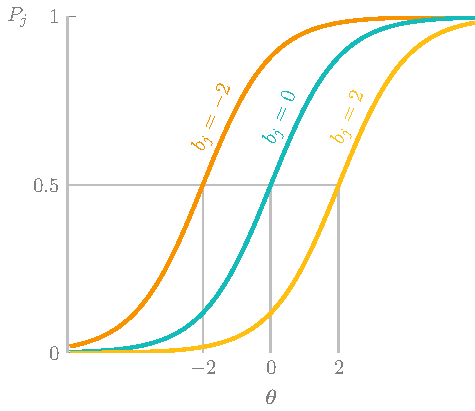
\includegraphics[page=1]{03-education/figures/tikzfigures.pdf}
    \caption[Item response functions of the 1PL model]{Three \glspl{irf} in the \gls{1pl} model, with different difficulty parameters $b_j$. The difficulty parameter represents the difficulty of the exercise. 
    For a fixed ability level, e.g. $\bm\theta = 0$, a higher difficulty means a lower probability $P_j$ of getting a correct answer.
    The probability of a correct answer is 50\% when $b_j = \bm\theta$.}
    \label{fig:1pl}
\end{figure}

There are more characteristics to an exercise than its difficulty. 
One characteristic that is useful to help estimate the ability of users is the discriminative ability of the exercise.
This characteristic represents how good an exercise is at differentiating between users of varying ability levels.
An extension to the \gls{1pl} model exists that includes this parameter, resulting in the \gls{2pl}. 
This second parameter $a_j$ of an item is a multiplicative parameter, as shown in the \gls{irf} in Equation~\ref{eq:2pl}.

\begin{equation}
    \label{eq:2pl}
    P_{j}(\bm{\theta}_i,\bm{p}_j) =
    Pr(X_{ij} = 1 | \bm{\theta}_i,a_j,b_j) =
    \frac{\exp\big[a_j(\theta_i - b_j)\big]}{1 + \exp\big[a_j(\theta_i - b_j)\big]}
\end{equation}

In Figure~\ref{fig:2pl} the \glspl{irf} are plotted for three exercises with the same difficulty $b_j = 0$ but various discriminative abilities. 
For all three \glspl{irf} the probability of a correct answer is still 0.5 for users with an ability level equal to the exercise difficulty.
However, the second parameter influences the steepness of the curve.
For larger discrimination parameters such as $a_3 = 4$, a smaller increase in ability $\bm\theta$ around the exercise difficulty level $b_j = 0$ leads to a more notable increase in probability of a correct answer $P_j$.
Such an exercise discriminates better between low and high ability users.
On the other hand, exercises with lower discrimination values, like $a_1 = 0.25$ result in flatter \glspl{irf} and do not allow as easily for such discrimination.

\begin{figure}
    \centering
    %\input{03-education/plots/2pl}
    \includegraphics[page=2]{03-education/figures/tikzfigures.pdf}
    \caption[Item response functions of the 2PL model]{Three \glspl{irf} in the \gls{2pl} model, with equal difficulty parameter $b_j$ but different discrimination parameters $a_j$. The discrimination parameter represents how well an exercise can differentiate between users of different ability levels $\bm\theta$. A higher value means a steeper increase in probability of a correct answer $P_j$ around the difficulty level $\bm\theta = b_j$.}
    \label{fig:2pl}
\end{figure}

%Figure~\ref{fig:its-architecture} shows the completed architecture of the \gls{its}, obtained by replacing the algorithmic components with the techniques explained in this section.
%
%\begin{figure}
%    \centering
%    \input{03-education/plots/its-filled}
%  \caption{todo}
%  \label{fig:its-architecture} 
%\end{figure}

\subsubsection{Model calibration}
Both the \gls{1pl} and \gls{2pl} models hold parameters of two types: item parameters $\bm{p}_j$ and person parameters $\bm{\theta}_i$. 
With enough data, both sets of parameters can be accurately estimated.
First, the item parameters are estimated independently of the ability levels, this is called the \textit{model calibration}. 
Next, the ability levels are estimated while keeping the item parameters fixed.

\Gls{irt} offers several model calibration techniques, mostly designed for item banks with several dozens of items.
The larger size of the item bank of \gls{scw} will cause longer execution times and more difficult convergence to stable estimates.
I solve this problem by splitting the item bank to several smaller item banks, for example one for each framework on the platform.
The resulting consequences are discussed in Chapter~\ref{ch:its-experiments}.

The calibration of the model consists of tuning the model parameters to maximize the likelihood of the observed data.
More formally, model calibration is maximizing the likelihood of the model $L(\bm\theta,\bm{p})$ with respect to all item parameters $\bm{p} = (\bm{p}_1,\dots,\bm{p}_J)$.
Because this likelihood is also dependent on all person parameters $\bm\theta = (\theta_1,\dots,\theta_I)$, direct maximization is not possible.
There are several possible techniques that can be used to overcome this.
The most well-known are \gls{jml}, \gls{cml}, and \gls{mml}~\cite{magis2017computerized}.

The \gls{jml} algorithm iteratively maximizes the full likelihood with respect to both person and item parameters until convergence is reached.

\Gls{cml} relies on properties specific to the Rasch model to replace unknown ability levels with known sufficient statistics which then allows for the estimation of the item parameters without requiring the estimation of the person parameters.

\Gls{mml} is formulated under the assumption that the ability is a random parameter.
In contrast to the \gls{cml}, it can be used for other \gls{irt} models besides the Rasch model~\cite{bartolucci2010point}.
It does not replace the person parameters by sufficient statistics, but aims to integrate out the person parameters from the maximization process~\cite{bartolucci2010point,magis2017computerized}.
A prior distribution for the ability parameters $f(\bm{\theta})$ is used to compute the marginal likelihood (or the expectation) of a response pattern as shown in Equation~\ref{eq:integrate-out}.

\begin{equation}
    \label{eq:integrate-out}
    P_{j}(\bm{p}_j) = \int_{\mathbb{R}} P_{j}(\bm{\theta}_i,\bm{p}_j) f(\bm{\theta}_i) d\bm{\theta}_i
\end{equation}

The prior distributions are often chosen as normal distributions.
The item parameters can then be estimated by maximizing the full likelihood, calculated as the product of all marginal pattern likelihoods.
Computing these marginal response pattern distributions was conceptually complex until efficient \gls{em} algorithms were implemented~\cite{magis2017computerized}.

In this work, I used the \gls{mml} approach as it has many advantages, such as its applicability to many types of \gls{irt} models, its ability to compare the fit of different models, and its ability to handle perfect response patterns (all correct or all incorrect answers).

\subsubsection{Ability estimation}
Once the item parameters are calibrated, they are set as fixed.
Estimating the person parameters is done through maximizing the \textit{likelihood function} shown in Equation~\ref{eq:wle1}, with respect to $\theta$. 

\begin{equation}
    \label{eq:wle1}
    L(\theta) = \prod_{j=1}^{J} \prod_{k=0}^{K_j} P_{jk}(\theta, \bm{p}_j)^{Y_{jk}}
\end{equation}

In this equation, $Y_{jk}$ equals one if the response category $k$ was chosen for item $j$ and zero otherwise.

Note that since the item parameters $\bm{p}_j$ are already calibrated and now set as fixed, the function only depends on the person parameters $\theta$.
Maximizing this function is equivalent to maximizing its logarithm, the so-called \textit{log-likelihood function}, as shown in Equation~\ref{eq:wle2}.

\begin{equation}
    \label{eq:wle2}
    l(\theta) = \sum_{j=1}^{J} \sum_{k=0}^{K_j} Y_{jk}\log P_{jk}(\theta, \bm{p}_j)
\end{equation}

For dichotomous items ($k \in \{0,1\}$), such as in our case, this can be written as:

\begin{equation}
    \label{eq:wle3}
    l(\theta) = \sum_{j=1}^{J} Y_{j1} \log P_{j}(\theta, \bm{p}_j) + Y_{j0} \log Q_{j}(\theta, \bm{p}_j)
\end{equation}

%\todo[inline]{I think this would be too much of a tangent on the actual work}
There are several calibration methods to maximize this likelihood, describing them is out of the scope of this book. 
The method applied in this work is the \gls{wle}~\cite{magis2017computerized}.

\subsection{Alternative approaches}
\gls{irt} is often used to adapt the learning material to the ability level of the student in e-learning systems~\cite{chen2005personalized,yarandi2011personalised}.
Often the \gls{irt} ability level is used to determine the appropriate difficulty level of the exercises that should be presented to the user~\cite{chen2005personalized,yarandi2011personalised,khanal2020systematic}.
In another approach the \gls{irt} ability level was used as a weight in \gls{cf} algorithms so that that the users with greater ability level have greater weight in the calculation of the recommendations than the users with less knowledge.
This approach assumes that users of greater ability level, such as teachers, are more able to assess the utility of an item than users of lower ability level.
In this work, however, users do not rate the items explicitly but instead the utility is determined from learning outcome and engagement, as will be explained in Section~\ref{sec:utility}.

Despite the popularity of \gls{irt} some alternative approaches exist to determine the ability level of a user.

\subsubsection{Classical Test Theory}
In \gls{ctt}, all users have to complete the same exercises and their accuracy on the questions is used as an indicator for the ability level.
Classic test theory assumes that each person has an unobservable true ability score $T$ that would be the result of a test if there are no errors in the measurement.
In a test, the observed score $X$ is measured instead.
This score is defined as the sum of the true score and a measurement error $E$.
According to \gls{ctt}, the true score is impossible to obtain, but several techniques exist to estimate the reliability of a test.

Besides the lower accuracy of ability estimation, \gls{ctt} is also not appropriate to use in the \gls{its} because it requires fixed item selection for all the users.
By doing this, some users are guaranteed to feel bored or frustrated since it is impossible to select items of the appropriate difficulty level for all of the users simultaneously.

\subsubsection{Other IRT models}
\paragraph{Three- and four-parameter logistic models}
In this work we are using the \gls{2pl} Rasch model of \gls{irt}.
However, further extensions exist on the \gls{2pl} model that add additional parameters.
The \gls{3pl} and \gls{4pl} add parameters that influence the lower and upper asymptotic behaviour of the \gls{irf}~\cite{magis2017computerized}.
The lower asymptote parameter $c_j$ is sometimes called the pseudo-guessing parameter. 
It allows the probability of a correct answer for infinitely small ability levels to be a positive probability instead of zero in the \gls{1pl} and \gls{2pl} model. 
Even users of extremely low ability level still have a non-zero probability of answering the exercise correctly.
In reality, this can of course be achieved through guessing the correct answer in case of multiple-choice.

On the opposite side of the curve, the upper asymptote parameter $d_j$ allows the maximal probability to be lower than one. 
This parameter is called the inattention parameter. 
The \gls{4pl} model allows users of extremely high ability level to have a probability of less than 1 of answering the exercise correctly.
This can be explained as the user being inattentive or hurried when answering the question.

The resulting \glspl{irf} are shown in Equations~\ref{eq:3pl} and \ref{eq:4pl}.
\begin{equation}
\begin{split}
    \label{eq:3pl}
    P_{j}(\bm{\theta}_i,\bm{p}_j)
    & = Pr(X_{ij} = 1 | \bm{\theta}_i,a_j,b_j,c_j) \\
    & = c_j + (1-c_j) \frac{\exp\big[a_j(\theta_i - b_j)\big]}{1 + \exp\big[a_j(\theta_i - b_j)\big]}
\end{split}
\end{equation}
\begin{equation}
\begin{split}
    \label{eq:4pl}
    P_{j}(\bm{\theta}_i,\bm{p}_j) =
    & = Pr(X_{ij} = 1 | \bm{\theta}_i,a_j,b_j,c_j,d_j)\\
    & = c_j + (d_j-c_j) \frac{\exp\big[a_j(\theta_i - b_j)\big]}{1 + \exp\big[a_j(\theta_i - b_j)\big]}
\end{split}
\end{equation}

\Glspl{irf} of the \gls{3pl} model with varying pseudo-guessing parameters are plotted in Figure~\ref{fig:3pl}.
In Figure~\ref{fig:4pl}, three \glspl{irf} are plotted with varying values for the inattention parameter.
The addition of these parameters is likely to improve the fit of the model to the data.
However, the pseudo-guessing and inattention parameters of exercises are not of much use in the \gls{its} or the \gls{scw} portal in general, and hence the \gls{2pl} model is chosen.

\begin{figure}
    \centering
    %\input{03-education/plots/3pl}
    \includegraphics[page=4]{03-education/figures/tikzfigures.pdf}
    \caption[Item response functions of the 3PL model]{Three \glspl{irf} in the \gls{3pl} model, with equal difficulty and discrimination parameters but different pseudo-guessing parameters $c_j$. The pseudo-guessing parameter represents the probability that a user is able to guess the correct answer to a question. A non-zero pseudo-guessing parameter means a non-zero probability of a correct answer $P_j$, even for users of extremely low ability level $\bm\theta$.}
    \label{fig:3pl}
\end{figure}

\begin{figure}
    \centering
    %\input{03-education/plots/4pl}
    \includegraphics[page=5]{03-education/figures/tikzfigures.pdf}
    \caption[Item response functions of the 4PL model]{Three \glspl{irf} in the \gls{4pl} model, with equal difficulty, discrimination, and pseudo-guessing parameters but different inattention parameters $d_j$. The inattention parameter represents the probability that a user answers incorrectly due to inattention. A inattention parameter different form 1 means that the probability of a correct answer $P_j$ is never 1, not even for users of extremely high ability level $\bm\theta$.}
    \label{fig:4pl}
\end{figure}

\paragraph{Polytomous IRT models}
%Predict WHICH of the answers is given (in multiple choice). For that it is necessary to know which one is MOST correct. Unfortunately this information is not available.
% The selection of a particular polytomous model involves a number of factors: the type of data, model-
%data fit, philosophical considerations, model assumptions, and parsimony. If the data consist of items that have unordered alternatives, then the NRM is appropriate. When responses to an item are classified into more thantwo categoriesthatcan beorderedtorepresentvaryingdegreesofthetraitmeasuredbytheitem, theneithertheGRM,GPCM,orthePCMcouldbeused.Iftheordereddataareratings,thenmoreconstrained versionsofthesemodels,suchastheMRSM,theSIM,ortheARSM,wouldbeappropriate.~\cite{dodd1995computerized}
In the \gls{2pl} model, we are only concerned with whether or not the selected answer is correct.
However, even if an incorrect options is selected, it is often possible to use this information to refine the estimate of the ability level of the user based on which incorrect option was chosen~\cite{magis2017computerized}.
This is the intent of polytomous \gls{irt} models.
There are many polytomous models available but they generally require scoring in a way that partial credit can be given for incorrect answers~\cite{dodd1995computerized}.
This makes sense if one considers scoring essays based on quality, or giving partial credit in mathematical questions for completing some of the steps.

On the \gls{scw} portal this could be achieved by ranking the options in the multiple choice question from the most incorrect to the most correct.
However, currently this is not the case, so we have no indication of which incorrect answer is closest to correct.
Furthermore, historically the incorrect answers have not been logged in the data collection, only the amount of incorrect guesses before a correct answer is given.
In case the user gave up before finding the correct answer (or in assessments where only one guess is available), the last guess is logged.
Polytomous models could result in more accurate results, however, currently they can not be used to the available data set.

\paragraph{Multidimensional IRT models}
While the ability level has been introduced as a multivariate vector of latent traits $\bm{\theta}_i$, in Section~\label{sec:irt-intro}, in the current implementation this has been implemented as a scalar.
In reality, the ability of a user regarding software security is not accurately represented as a single value.
When the ability estimate is represented as a vector, a value can be obtained for each dimensions of the skill.
For example, the ability of a user for each of the vulnerability categories can be represented as a scalar.
Using a multidimensional representation for the ability level like this, is not only likely to result in more accurate estimates, but also allows more granular decision making of the appropriate difficulty for an item in the \gls{its}.
However, sufficient data needs to be available to have an accurate measurement for each of the dimensions which would limit the amount of users that can be accurately assessed.
I have opted to keep as much data as possible to train the \gls{cf} algorithm instead.

\paragraph{Response-time IRT models}
Response-time \gls{irt} models also take into account how much time each user takes to answer a correct answer.
However, as mentioned before, there have been several bugs present in the time tracking features on the platform and this data is currently unreliable.

Furthermore, time pressure varies in different modes on the platform.
While users can generally take as much time as they prefer when answering questions in training and assessments, in tournaments there is a limited time to complete the questions.

\subsubsection{Elo system}
The Elo rating system, named after its inventor Arpad Elo, is a method for calculating relative skill levels between players of a zero-sum game~\cite{elo1978rating}.
It is widely used in sports, games, and videogames, such as chess, American football, basketball, Major League Baseball, table tennis, Scrabble, Counter Strike: Global Offensive, and League of Legends.

Similarly to \gls{irt}, the ability level is not measured directly, but it is inferred from wins, losses, and draws against other players or teams.
Based on the current ability levels, the expected outcome of a match-up is predicted.
When the actual outcome differs from this expectation, the ability level is updated~\cite{elo2008logistic}.
By how much it is updated depends on the difference between the ability levels, and in some cases by the observed skill difference.
For an overwhelming victory a bigger increase in ability will often be awarded than for a near win.

The Elo system is made for symmetric matchups, player versus player, or team versus team.
A zero-sum game is a mathematical representation of a situation in which an advantage that is won by one player is lost by the other.
While \gls{irt} sets both users and items on the same scale, the training platform can not be considered a zero-sum game.
One challenge is played by many more players than a single player usually plays challenges.

Although adaptations exist for asymmetric games~\cite{wise2021elo}, I expect the ability estimates to converge slower and the difficulty estimates of items to be less stable than with \gls{irt}.
\Gls{irt} takes into account the entire response pattern, hence it is able to estimate the outcome of a challenge again later, based on new information.
The Elo system only takes into account the current ability of the user, which might still be inaccurate at the time of playing.
As a result, potentially large updates are made to the difficulty of the items that are presented to this user.
\section{Data}
\label{sec:data}

The data used to create the \gls{its} is extracted from the developer log of the \gls{scw} training platform.

While this database was not originally intended to be used for analytics, and other data sources have been set up since, lots of useful data is present in this database and it is by far the largest collection. 

Each challenge on the platform has a unique \gls{id}.
This \gls{id} is tied to the \gls{vulnerability} in a code fragment, not to the way it is presented to the user (L1-L5).
For each challenge the language and framework are known, as well as the category and subcategory of the vulnerability.
The difficulty assigned to this challenge is also known but it is not an accurate representation.
The way this difficulty is determined is explained in more detail in Appendix~\ref{app:challenges}.

The multiple choice options for a identify and locate challenges are randomly generated each time it is presented to a user on the website.
For the fix challenges the multiple-choice options are fixed, and determined by the author of the challenge.
There is no clear order to the multiple-choice options.
There is only one correct option, and all others are incorrect, with no distinction between which incorrect option is the closest to the correct one, or the most misleading option.

Each user has a unique \gls{id} that is a hashed, this way it is not possible to identify the person behind this user \gls{id} in compliance with the \gls{gdpr}.
Some information on the user is available, but it is not used in the design of the \gls{its}.
For example, the time zone and the chosen country as the \textit{home base} in the gamification features.
For each user it is also possible to look up information about the company they are working for, such as the size of the company and its main industry.

\subsection{Data collection}
Whenever a user tries to solve a challenge, a number of variables is written to the developer log.
For each challenge attempt, the unique user \gls{id} is logged, as well as the challenge \gls{id} and the way this challenge was presented to the user (L1-L5).
Each play mode (tournament, training, assessment) is logged in a separate collection.
A number of performance metrics are logged as well, such as the outcome (correct or incorrect), the amount of attempts needed, and the amount of hints used.

The time spent to complete the challenge is logged as well.
However upon inspecting this, there seem to have been several bugs present in the past, making this metric not usable.
Furthermore, even for the more recent data where these bugs have been resolved, there is no way to find out whether the user was actively trying to solve the challenge during this time, or doing something else.
It is also not possible to know how much of this time was spent reading the hints.

More than 12 million challenge attempts have been written to the developer log.

\subsection{Data pre-processing}
This vast collection of data includes users who only completed a small number of challenges, such as during the free trial.
For these users, we cannot accurately predict their ability level, nor can we learn much about their preferences.
Both the \gls{cf} algorithm and the Rasch model are only successful when the user has a sufficiently long history on the platform.
For this reason, we are only using challenge attempts done by users who completed at least 20 challenges, a recommended minimum length to achieve reasonable accuracy for the Rasch model.
Users who have completed at least 20 challenges will be called active users from here on.
Out of the 175,979 unique users who have completed at least one challenge on the platform, 95,591 are considered active users whose behaviour on the platform will be used to create the \gls{its}.

A similar argument can be made for the challenges.
To accurately calibrate the difficulty of a challenge, enough users of varying ability levels need to complete it.
The ability level of these users needs to be known.
To calibrate the difficulty of an exercise, \gls{irt} recommends a minimum of 500 responses to an item.
As a result we are filtering out all challenges that are not completed by at least 500 active users.
Out of the 19,782 exercises 9,144 remain, 40 of the 50 frameworks are still represented in this data set.
On the \gls{scw} training platform, there are multiple modes, each with their own rules.
In training and tournament, hints are available and multiple attempts are allowed, while in assessments there is only one attempt possible.
The Rasch model, on the other hand, expects dichotomous responses.
To map challenge attempts of all modes fairly to this binary outcome, any challenge attempt is only considered correct if it was answered correctly without use of any hints on the first attempt.
In the rest of this book this will be implied when it is written that a challenge is answered correctly.

\subsection{Data annotation}
\label{sec:utility}
The exercise difficulties and user ability levels as estimated by the Rasch model can be used to determine the utility of an item for a user.
A scale of 1 - 5 was chosen, and each item is assigned a neutral utility of 3 by default.
This utility is updated based on the performance of the user on this item, and on related items later in time.

\paragraph{Flow}
The first influence on the utility of an item is user engagement.
If the item is considered likely to keep the user in flow, its utility is decreased.
If the item is likely to make users feel frustrated or bored, its utility is increased.
Whether or not an item is likely to keep a user in flow is calculated using the probability of a correct answer.
Before each item is played, the difficulty of this item and the current ability level of the user are used to determine this probability through the \gls{irf}.
The utility is then updated based on this probability as well as the actual outcome of the answer.
If the probability of a correct answer is lower than 50\%, and the user did indeed answer the item incorrectly, this item's utility is lowered for risk of frustration.
If, on the other hand, the probability of a correct answer is larger than 80\% and the item is answered correctly, this item's utility is lowered for risk of boredom.
These values are in line with research on the engagement of examinees in \glspl{cat}~\cite{ling2017computerized}\todo{more refs}.
The utility in both these cases is decreased by one.

This decrease in utility is immediately nullified if the next item is played in short succession.
When the next item is played within 40 minutes, the upper scale of a reasonable play time for a challenge, the utility of the previous item is increased by one, as a reward for this apparent engagement\todo{rephrase?}.

\paragraph{Increased ability}
If a user learns something new from an item, this should also lead to increased utility.
However, with \gls{irt}, and any other approximation methods, the estimate of the ability is never increased based on an incorrect answer.
The only reason to increase the ability estimate, is when there is evidence of this increase, i.e. when the user answers a difficult item correctly.
In reality, however, learning takes place before this correct answer, and the actual (unobservable) ability level has increased earlier in time, so that the user was able to answer this difficult item correctly.
In line with this observation, items are updated retrospectively based on answers to related items later in time.

If an item is answered correctly, the utility of the previous item in the same vulnerability category is increased based on the difference in difficulty.
Similarly, the utility of the previous item in the same category is decreased for an incorrect answer.

Putting the rewards and punishments for flow and increased ability together results in the final algorithm to determine the utility of an item as shown in Algorithm~\ref{al:utility}.
The \texttt{min} and \texttt{max} functions are added to ensure utility ratings stay within the 1 - 5 scale.

\begin{algorithm}[H]
\caption{\label{al:utility}Utility of challenges}
\SetAlgoLined
\SetKwInOut{Input}{input}
\SetKwInOut{Output}{output}
\Input{current item $i$\\ probability of correct answer $p$}
\Output{utility $u_j$, for items $j \leq i$}
$u_i \leftarrow 3$\\
\lIf{$i-1$ played less than 40 minutes ago}{$u_{i-1} = u_{i-1} + 1$}
\uIf{$i$ answered correctly}
    {
    \lIf{$p > 0.8$}{$u_i = u_i - 1$}
    \lIf{$d_i$ > $d_j$}{$u_j = \text{min}(5, u_j + (d_i - d_j))$}
    }
\Else
    {
    \lIf{$p < 0.5$}{$u_i = u_1 - 1$}
    \lIf{$d_i$ < $d_j$}{$u_j = \text{max}(1, u_j + (d_i - d_j))$}
    }
\end{algorithm}

Annotating the items like this results in a reasonable distribution of the ratings.
A large portion of the items is rated around the middle rating of 3, but a significant amount of items also end up with a lower or higher rating.
A clear bias exists for some users, for whom the ratings are either consistently higher or consistently lower.
This can be explained by the (mis)match between these users' ability levels and the current item selection of the default courses or tournaments.
Some users have an ability level that is much higher, and they are consistently shown items that can be considered too easy for them, resulting in consistently lower ratings.
For other users, the current selection happens to be about right for their skill level, and hence their ratings are consistently somewhat higher.
\chapter{Experiments}
\label{ch:its-experiments}

Several techniques and algorithms have been combined in the design of the \gls{its}.
With the implementation and evaluation of each of these, new insights were gained into the mental model of the developer. 
In this section, I describe the four experiments I conducted to evaluate and fine-tune each component in the \gls{its}.

\summarybox{
In the first experiment, I evaluated the results of the Rasch model through statistical analyses.
I found that the assigned difficulty of an exercise on the \gls{scw} platform does not accurately represent the actual difficulty as experienced by the users.
The statistical tests show that the actual difficulty does depend on the framework of the exercise, the category of the vulnerability, and the presentation of the exercise to the user. 

The second experiment showed that out of the tested approximation methods, the one invented in this work is the best to achieve a fast ability estimates at each point in time.
The mean error stays below 10\% even after more than 200 completed challenges.

In the final two experiments, I tested the performance of different \gls{cf} algorithms and their adaptations to learning systems.
The adaptations caused an increase in predication accuracy between 3.9\% and 13.7\%, depending on the algorithm.
The best performing algorithm in the end is the \gls{knn} baseline algorithm, achieving a mean absolute error of 0.4206.
}

\section{Rash model}
\label{sec:eval-rasch}

\subsection{Goals and research questions}
The main \textit{goal} of the first experiment is to discover correlations between the difficulty of an exercise as estimated by the Rasch model, and characteristics of that exercise.
The \textit{purpose} is to gain insights in the mental model of the developer, and discover which languages, frameworks, or vulnerability types are typically more difficult.
The results of this experiment can be used in the \gls{its} to approximate the difficulty of an exercise when there is no sufficient data available to obtain an estimate with \gls{irt}.

The above goal can be achieved by means of an experiment aimed at answering the following questions:
Is there a statistically significant correlation between the difficulty of a challenge and its
\begin{itemize}
    \item \textbf{Q1} assigned difficulty on the \gls{scw} platform?
    \item \textbf{Q2} vulnerability category?
    \item \textbf{Q3} vulnerability type (subcategory)?
    \item \textbf{Q4} language and framework?
    \item \textbf{Q5} presentation form (locate, identify, fix)?
\end{itemize}

It is expected that the last four characteristics have a significant influence on the difficulty of a challenge.
Some vulnerabilities are more difficult to detect, understand, or fix than others.
This is evident, for example, from the \gls{owasp} Top 10 pages, where each category is assigned a score for exploitability, prevalance, detectability, and technical impact.
There is no clear explanation as to how these scores are determined.
Personal and anecdotal evidence also shows that it is more difficult to get security right while working in certain languages and frameworks.

The first variable, the assigned difficulty on the \gls{scw} platform, is expected to have little impact on the actual difficulty.
As explained in Appendix~\ref{app:challenges}, this difficulty only represents the likelihood of a correct answer in case of a blind guess.
It does not take into account the contents of the exercise, only the number of options to choose from.
While the amount of options is expected to have some influence on the actual difficulty, this effect is likely to be small compared to other characteristics of the exercise.

\subsection{Experimental set-up}
In Section~\ref{sec:calib} it was previously mentioned that calibration techniques for the Rasch model are mostly designed for item banks with several dozens of items.
The larger size of the item bank of \gls{scw} will cause longer execution times and more difficult convergence to stable estimates.
I solved this problem by splitting the item bank into several smaller item banks and calibrating each of them separately.

The downside to this approach is that the Rasch model does not use an absolute scale.
This is evident from the equation for the \gls{1pl} model in Equation~\ref{eq:1pl}, repeated here for convenience in Equation~\ref{eq:1pl-2}.

\begin{equation}
    \label{eq:1pl-2}
    P_{j}(\bm{\theta}_i,\bm{p}_j) =
    Pr(X_{ij} = 1 | \bm{\theta}_i,b_j) =
    \frac{\exp(\theta_i - b_j)}{1 + \exp(\theta_i - b_j)}
\end{equation}

Adding or subtracting the same value from both the difficulty parameter $b_j$ and the ability level $\theta_i$ will cancel out and result in the same probability of a correct answer $P_j$.
In other words, the origin of the scale can be chosen arbitrarily.
In practice, the origin is often set to the mean of the ability estimates~\cite{magis2017computerized}.
I used the R package \texttt{TAM} to estimate the item and person parameters~\cite{robitzsch2021package}.
In the documentation of this package there is no information about the chosen scale.
Based on the implementation that is available on GitHub\footnote{\url{https://github.com/cran/TAM/blob/master/R/tam.mml.2pl.R}}, the scale is set to the mean of the difficulty estimates after the first iteration of the calibration process.
For each item bank that is calibrated separately, the results can hence not be easily compared to other item banks, as they each have their own scale.

However, for this experiment it is necessary to compare the difficulty of challenges across the entire platform.
To be able to do this, the entire item bank has to be calibrated at once. 
The necessary computations took over 73 hours to complete, confirming once more that it would not be feasible to use in the \gls{its}.

\subsubsection{Statistical significance}
With this single Rasch model calibrated, there is a difficulty estimate for every challenge on the platform.
It is now possible to group these challenges according to different characteristics and compute the mean difficulty of each group.
Before we can compare the mean difficulties for each characteristic, however, the results have to be tested for statistical significance.

Which test can be used to do this, depends on the values each characteristic can take.
The difficulty as assigned on the \gls{scw} platform takes on values between 0 and 100, and is hence a numerical variable.
The vulnerability category, vulnerability type, framework, and presentation form are each categorical variables.
Each of these characteristics can only take a limited number of categorical values.

To test the correlation between the difficulty on the \gls{scw} training platform and the \gls{irt} difficulty, the coefficient of determination (R-squared) can be used, as both variables are numerical variables.
The test (R = 0.03, $p = 1.85 \times 10^{-3}$) determines that no significant variation in the \gls{irt} difficulty can be explained by the \gls{scw} difficulty.
This is no surprise, it is clear that the current difficulty assigned on the platform is not an accurate representation of the actual difficulty.

A one-way \gls{anova} can be used for the categorical variables.
This test determines if there is a statistically significant difference between one or more of the possible values that a categorical variable can take.
The one-way \gls{anova} compares the mean difficulty for each of those values and determines whether any of those means are statistically significantly different from each other.
If the one-way \gls{anova} returns a statistically significant result, that means there are at least two values that are statistically different from each other.

The variables were found to have unequal variances across the possible values, a property called heterogeneity of variances.
A Welch \gls{anova} should hence be used, as this \gls{anova} can better control for type I errors~\cite{liu2015comparing}.
The results of the Welch \glspl{anova} are shown in Table~\ref{tab:anova1} and show that a statistically significant difference exists between values for each of the categorical variables.

\begin{table}
    \centering
    \caption[\Gls{anova} test results for Rasch model]{The results of one-way \gls{anova} tests between variables of the exercises and the estimated difficulty. For each variable, the degrees of freedom (df) are shown, as well as the F-statistic, the $p$-value, and the eta-squared ($\eta^2$). All four categorical variables have statistically significant correlations with the estimated difficulty of the exercise. The presentation has a large effect on the estimated difficulty. The category, vulnerability, and framework each have a medium effect.}
    \setcellgapes{4pt}\makegapedcells
    \begin{tabular}{l l S[table-format=3.3] l l}
Variable & df & F & $p$ & $\eta^2$ \\
    \hline
    Category & 36 & 14.154 & $2.97 \times 10^{-53}$ & 0.046 \\
    Vulnerability & 142 & 5.393 & $1.19 \times 10^{-45}$ & 0.079 \\
    Framework & 38 & 11.430 & $ 1.49 \times 10^{-41}$ & 0.060 \\
    Presentation & 3 & 346.164 & $3.00 \times 10^{-6}$ & 0.155 \\
    \end{tabular}
    \label{tab:anova1}
\end{table}

In this \gls{anova} the eta-squared ($\eta^2$) metric was used to measure the effect size of each categorical variable on the estimated \gls{irt} difficulty.
A medium effect was measured for the framework, category, and vulnerability of the exercise and a large effect was measured for the presentation.

Pairwise Games-Howell post-hoc tests were then used to determine which of the values in each categorical variable are statistically different from each other~\cite{games1976pairwise}.
Results of these tests are shown in Table~\ref{tab:gameshowell}.

\begin{table}
    \centering
    \caption[Pairwise Games-Howell post-hoc test results]{The second column displays the number of possible values. Every one of those values is paired with all other values for a pairwise Games-Howell test. The next two columns report the amount of pairs for which the means differ in a statistically significant way, and the amount of pairs for which this is not the case. In the final column the number of values is shown, for which at least one pair exists where the means are statistically significantly different.}
    \setcellgapes{4pt}\makegapedcells
    \renewcommand\theadfont{\normalsize}
    \begin{tabular}{l l l l l}
    Variable & \thead{Values} & \thead{Significant\\ pairs} & \thead{Insignificant\\ pairs} & \thead{Significant\\ values} \\
    \hline
    Category & 36 & 118 & 548 & 29 \\
    Vulnerability & 142 & 384 & 9769 & 77 \\
    Framework & 38 & 217 & 524 & 37 \\
    Presentation & 3 & 3 & 0 & 3 \\
    \end{tabular}
    \label{tab:gameshowell}
\end{table}


With the exception of the presentation, each of the categorical variables has a number of values that do not show a statistical significance with any other value.
If there is no statistical significant difference between two values, this is usually due to insufficient data for one of the values or because the data of one (or both) of the values is too widely spread and there is significant overlap between the data for the two values.
%In the remainder of this section such values are not discussed or shown in any of the graphical displays.
The remaining values show a statistically significant difference in mean difficulty with at least one other value.
When mean difficulties are compared in the remainder of this section, only values are compared whose means show statistically significant differences as determined by the pairwise Games-Howell tests.
Each of the values that are compared explicitly, show statistically significant differences in mean difficulty with a $p$-value of at most 0.05.
The exact $p$-values of these tests are reported in Appendix~\ref{app:pairups}.
%Where appropriate, the $p$-values of the pairwise Games-Howell test for compared categories will be included.

\subsection{Findings}
In this section, I report some of the notable differences in difficulty between different values for each of the characteristics and offer possible explanations for these observations.

\subsubsection{Vulnerability category}
There is a statistically significant difference between the mean difficulty of the four hardest and the four easiest categories.
When comparing these categories to each other, as shown in Figure~\ref{fig:cats1}, their difficulty seems mostly related to the locality of the vulnerability type.

\begin{figure}
    \centering
    %\input{03-education/plots/categories}
    \includegraphics[page=20]{03-education/figures/tikzfigures.pdf}
    \caption[Difficulty of bugs versus flaws]{Vulnerabilities that often require only local changes to the code to fix have lower mean difficulties.}
    \label{fig:cats1}
\end{figure}

The top four categories are (design) \glspl{flaw}, and the fix often involves larger pieces of code.
This is especially the case for business logic flaws and denial of service, where the complexity of the code is the main cause of the problem.
In these categories the developer is unable to foresee unintended results that are a direct result of the logic of their code.
%Some examples are logical errors, uncaught error handling, and problems with regular expressions.

The fixes of the four easiest categories usually only require local changes to the code.
Injection and \gls{xxe} are often fixed by properly sanitizing or whitelisting input parameters, or by configuring components properly.
Security problems related to session management are things like incorrect session lengths, insufficient entropy, or insufficient length for the session \glspl{id}.
Use of vulnerable components is most frequently fixed by updating to a version of the component where the vulnerabilities are fixed.
To fix these vulnerabilities, only local changes to the code are necessary, identifying the correct fix out of several options only involves building a mental model of a small piece of code, making it easier to reason about.

Still, it is noteworthy that the categories near the bottom of the scale are some of the most infamous vulnerabilities.
Injection for example is the top category of the \gls{owasp} top 10 in 2017 and receives high scores for exploitability, detectability, and technicality.
It has currently dropped to the third position in the draft of the next iteration to be released in 2021\footnote{\url{https://owasp.org/Top10/}}.
Based on our training data, at least, it seems that these scores might be exaggerated.
%To explain this, we have to consider the exercises on the \gls{scw} platform.
%To locate a vulnerability in the code, the category of the vulnerability is given.
%At the same time, these vulnerabilities are related to very specific pieces of code. \gls{sql} injection for example can only occur in database queries.
%This makes locating the vulnerability easier.
One exception to this is \gls{xss}.
Despite its infamy, it is closer to the middle of the scale, as can be seen in Figure~\ref{fig:cats2} where \gls{xss} is shown together with all categories it shows statistically significant differences with.
\Gls{xss} being in the middle of the scale can be explained by the fact that there are two major types of \gls{xss}, stored \gls{xss} and reflected \gls{xss}. 
In the case of reflected \gls{xss} the vulnerability is rather local, and the fix is also applied locally, by using output encoding.
For stored \gls{xss} there are usually multiple code fragments involved, one or more where the user input is stored as data and one or more where the stored data is used without output encoding.

In conclusion, the difficulty of the vulnerability correlates to the size of the related code fragments.
Vulnerabilities that only require local changes in the code to fix are easier to understand and fix in training, despite their apparent prevalence in practice.

\begin{figure}
    \centering
    %\input{03-education/plots/categories}
    \includegraphics[page=21]{03-education/figures/tikzfigures.pdf}
    \caption[Medium mean difficulty for XSS challenges]{Challenges about XSS show a mean difficulty around the middle of the scale.}
    \label{fig:cats2}
\end{figure}

\subsubsection{Framework}
Of the 38 different frameworks, 37 show statistically significant differences with at least one other framework.
Pseudocode shows a significant difference with 17 of these frameworks, all of which have a higher mean difficulty.
This makes sense as pseudocode is an artificial language.
It is designed to teach developers algorithms and other programming concepts, and should be easy to understand.

Memory management in memory-unsafe languages such as C and C++ can lead to a whole class of security problems that are avoided in memory-safe languages.
We can see this effect in the higher mean difficulty of C and C++ compared to those of the modern, memory-safe programming languages Java, C\# (.NET), and Python, as shown in Figure~\ref{fig:frames1}.
However, the memory-safe language Cobol also shows a statistically significantly higher mean difficulty compared to each of these three languages.
While Cobol is memory-safe, it does still require memory management and use of pointers, which might explain the higher mean difficulty.
Cobol is also known for its lack of clear documentation regarding security concepts.

\begin{figure}
    \centering
    %\input{03-education/plots/frameworks1}
    \includegraphics[page=9]{03-education/figures/tikzfigures.pdf}
    \caption[Memory-safe versus memory-unsafe languages]{Older programming languages require memory management and use of pointers. They show harder mean difficulties than languages that have automated memory management.}
    \label{fig:frames1}
\end{figure}

Several frameworks show statistically significant differences between the framework and its standard programming language.
This is the case for Java Spring, Java \gls{ee}, Java \gls{jsf}, C\# (.NET) Web Forms, and Python Django.
All of these frameworks are more difficult than their standard language counterparts, as shown in Figure~\ref{fig:frames2}.
This is surprising, as frameworks are designed to implement commonly used functions so that the developer does not have to.
For example, to securely hash a password in standard Java, the developer has to research which algorithm is the most secure, they have to generate a salt using a secure random number generator and correctly combine each of these techniques.
In Java Spring a \texttt{PasswordEncoder} interface is provided, the documentation of this interface is brief and informs developers that \texttt{BCryptPasswordEncoder} is the preferred implementation\footnote{\url{https://docs.spring.io/}}.

Because frameworks often automate these commonly used features, some details of the implementations might be lost to developers.
When the implementation is insufficient, or when the framework is used incorrectly, it is possible that even a security conscious developer can remain unaware of the consequences.
On top of the standard language skills, and the security knowledge, a developer using a framework hence also needs an intimate knowledge of the framework itself to deliver secure code.

\begin{figure}
    \centering
    %\input{03-education/plots/frameworks2}
    \includegraphics[page=10]{03-education/figures/tikzfigures.pdf}
    \caption[Frameworks versus default languages]{All of the frameworks that show statistically significant differences with their standard programming language, have a higher mean difficulty.}
    \label{fig:frames2}
\end{figure}

The mobile framework Java Android is more difficult than web frameworks for the same language (Java \gls{jsf}, Java Spring), as shown in Figure~\ref{fig:frames3}.
This can be explained through the increased attack vectors of mobile applications that are installed on the device of the user.
Because the device and operating system cannot be trusted, the developer has to be aware of other threats, such as restoring backups that are tampered with, detecting root access, and tapjacking.
Unfortunately, Objective C, an extension of C that can be used for mobile development, does not show a statistically significant difference with C itself to confirm this correlation.
The more modern replacement for Objective C, Swift, that is inspired by both C\# (.NET) and Python does show a statistically significant higher mean difficulty than both these languages~\cite{nondot}.

Languages and frameworks have evolved to automate some of the tasks of the developer, such as memory management, and password encryption.
The abstractions provided by these languages and frameworks does not always have a positive impact on security, as is evident from these results.
It is likely that the developers has to sufficiently grasp the implementation details to fully understand the security impact of their code.

\begin{figure}
    \centering
    %\input{03-education/plots/frameworks3}
    \includegraphics[page=11]{03-education/figures/tikzfigures.pdf}
    \caption[Mobile versus web frameworks]{Mobile framework and languages that show statistically significant differences with their web counterparts have higher mean difficulties.}
    \label{fig:frames3}
\end{figure}

\subsubsection{Presentation}
A challenge can be presented to the user as an identify, locate, or fix exercise.
It is unsurprising that identifying a vulnerability that is already marked in the code, is the easiest type of exercise, as shown in Figure~\ref{fig:presentation}. 
On the platform this type of exercise is usually the first stage of a two-stage challenge, with the second stage a fix exercise.

\begin{figure}
    \centering
    %\input{03-education/plots/frameworks3}
    \includegraphics[page=22]{03-education/figures/tikzfigures.pdf}
    \caption[Mean difficulty of challenge presentation]{The mean difficulty of each presentation form is statistically different of the other two. In line with observations in practice, locating a vulnerability in code is the most difficult of the three tasks, followed by fixing the vulnerability.}
    \label{fig:presentation}
\end{figure}

According to the Rasch model, locating vulnerabilities in the code is the most difficult task.
This is in line with observations made in practice, where many vulnerabilities go unnoticed by developers and are detected by automated tools at later stages in the \gls{sdlc}.
\section{Step size adjustment ability estimation}
\label{sec:eval-stepsize}

From the previous experiment in Section~\ref{sec:eval-rasch}, it is evident that calibrating the entire item bank takes a long time.
Similarly, computing the ability estimate based on the entire response pattern of a user takes too long.
Currently, about 15,000 challenges are completed every day, that is about one challenge every five seconds and this number is only expected to go up.
The computations to estimate the ability of a single user easily exceed that.
For a procedure that has to be executed this frequently, even a minute is too long.

\subsection{Goals and research questions}
The main \textit{goal} of this experiment is to evaluate different approximation procedures for the ability estimates.
The \textit{purpose} is to determine if they can be used to improve the efficiency of the ability computations without a significant loss in accuracy.
The \textit{quality focus} is the accuracy of the procedures with increasing numbers of answered items.
The above goal can be achieved by means of an experiment aimed at answering the following question for each procedure:
\begin{itemize}
    \item \textbf{Q1} how big is the mean error of the approximation after every 5 challenges?
\end{itemize}

\subsection{Approximation procedures}
In research literature, I have found two so-called step size adjustment procedures that are used in \glspl{cat}.
These procedures update the latest estimate based on either a fixed or variable step size~\cite{dodd1995computerized}.

\paragraph{Fixed step size} With a fixed step size, the ability estimate is increased (or decreased) by a specific amount, often between 0.4 and 0.7, when the user answers an item correctly (or incorrectly).
In this experiment the smallest step size of 0.4 is used for the evaluation.

\paragraph{Variable step size} With a variable step size the new ability estimate is placed at the halfway point between the current estimate and the difficulty of one of the two most extreme items in the item bank.
This is possible because the calibration techniques of \gls{irt} place users and items on the same scale.
If the user answers an item correctly, then the highest item parameter is used, if not, the lowest is used.
This procedure makes sense when one considers that the item selection algorithm in \glspl{cat} continuously selects items that are significantly above the current estimated ability level of the user, as explained in Section~\ref{sec:cf-alternatives}.
This is not the case for the historical data, and will also not be the case for the item selection of the \gls{its} in the future.
With more forgiving item selection this procedure will likely become inaccurate over time.

\paragraph{Adaptive step size} As an improvement, I have developed a variation of this procedure that uses the difficulty of the selected item instead of the difficulty of the extreme items in the item bank.
This adaptive step size procedure is shown in Algorithm~\ref{al:stepsize}.
When the user answers an item correctly that was expected to be hard, the ability estimate is increased to the halfway point between this item and the current estimate.
Similarly, when the user answers an item incorrectly that was expected to be easy, the ability estimate is decreased to the halfway point.

In the other cases, the outcome of the answer confirms that the current ability estimate is accurate.
A question that is more difficult than the user's current ability level is answered incorrectly, or a question below the ability level is answer correctly.
The player can then optionally be rewarded or punished with a fixed value, similar to the fixed step size adjustment procedure.
For this experiment, two variations of the adaptive step size procedure are tested, one with a fixed reward of 0.2 and one without a fixed reward.

\begin{algorithm}
\SetAlgoLined
\SetKwInOut{Input}{input}
\SetKwInOut{Output}{output}
\Input{user ability $\bm\theta_i$\\ item difficulty $\beta_j$ \\ answer $X_{ij}$ \\an optional punishment/reward value $r$}
\Output{updated user ability $\bm\theta_i$}
    \uIf{$X_{ij}$ is correct}{
        \uIf{$\bm\theta_i \leq \beta_j$}{return ($\bm\theta_i$ + $\beta_j$)/2}
        \Else{return $\bm\theta_i$ + $r$}
    }
    \Else{
        \uIf{$\bm\theta_i \geq \beta_j$}{return ($\bm\theta_i$ + $\beta_j$)/2}
        \Else{return $\bm\theta_i$ - $r$}
    }
\caption{\label{al:stepsize}Adaptive step size adjustment procedure}
\end{algorithm}

\subsection{Experimental set-up}
The different procedures are evaluated by comparing their approximations with the (accurate) estimated \gls{irt} ability.
To do this, an \gls{irt} ability estimate is needed for each user at each point in time, which requires many long-running \gls{irt} calibration procedures.
The five frameworks with the most data were chosen to use in the evaluation.
These are Java Spring, Java \gls{ee}, NodeJS Express, Pseudocode and Python Django.
The \gls{irt} ability was estimated for every user after every 5 completed challenges.

Each of the four procedures starts from the \gls{irt} ability estimate after 20 completed challenges.
From that point forward, the approximation methods are applied to the outcome of each challenge attempt.
The resulting approximations are compared to the \gls{irt} ability after every 5 challenges.

\subsection{Findings}
For each approximation method, the evolution of the mean error as a percent of the full ability scale, is shown Figure~\ref{fig:stepsize}.
The fixed step size adjustment becomes excessively inaccurate after only 15 to 20 challenges following the initial calibration.
After 200 challenges, the mean error of this approximation is up to 300\%.
While the adaptive step size procedure with a fixed reward is significantly better, its error still becomes excessively large and rises indefinitely.
The seemingly ever increasing error for these two procedures is explained by the large amount of users who play challenges that are below their skill level, and hence often answer them correctly.
With these two procedures, the ability level of users like this is increased each time, while these answers have no significant impact on the accurate estimates.

This effect is still visible for the variable step size adjustment procedure.
However, with this procedure the estimate does not exceed the difficulty of the most difficult item in the item bank, which limits the error to about 30\%.

The adaptive step size procedure without reward or punishment is the most accurate.
With this procedure, the ability estimate is not adjusted if the outcome of an item is as expected according to the current estimate.
The ability estimates of users who are answering easy items correctly is not updated.
For correct answers to difficult challenges or for incorrect answers to easy challenges, the estimate is moved in the right direction, but using smaller steps than the variable step size procedure.
The mean error of 10\% is acceptable for it to be used in the \gls{its}, as will become evident in a following experiment in Section~\ref{sec:eval-learning}.
This implies that the full calibration procedure is only necessary once, for the initial calibration.
In practice, the abilities for existing users will still periodically be re-calibrated along with the initial calibration of new users.

\begin{figure}
    \centering
    %\input{03-education/plots/stepsize}
    \includegraphics[page=13]{03-education/figures/tikzfigures.pdf}
    \caption[Error rates of step size adjustment procedures]{The error rates of the two procedures with a fixed step or a fixed reward become excessively large. For the variable step size procedure, the error rate is capped at around 30\%. The adaptive step size procedure without fixed reward is the most accurate and its error rate does not exceed 10\%.}
    \label{fig:stepsize}
\end{figure}

\section{Collaborative filtering algorithms}
\label{sec:eval-cf}

\subsection{Goal and research questions}
The main \textit{goal} of this experiment is to test the prediction accuracy of different (variations of) \gls{cf} algorithms.
The \textit{purpose} is to determine which algorithms are most effective at making recommendations on the \gls{scw} platform.
The \textit{quality focus} is the error of the predicted ratings compared to the observed ratings.
The above goal can be achieved by means of an experiment aimed at answering the following questions:
\begin{itemize}
    \item \textbf{Q1} What is a good error rate for this data set?
    \item \textbf{Q2} Which algorithm achieves the lowest error rate for predicting the utility of an item?
\end{itemize}

\subsection{Benchmark algorithms}
To train and evaluate different (variations of) algorithms, I have used the open-source Python scikit Surprise~\cite{Hug2020}.
Since it is open source, the code is available to download from GitHub and the implemented algorithms can later be adapted to learning systems.

Surprise provides two basic \gls{cf} algorithms that can be used as benchmarks to answer the first research question.

The first benchmark algorithm is called Normal Predictor, it estimates a normal distribution based on the training data and makes new predictions by randomly sampling from this distribution.

The second algorithm is the baseline algorithm.
It uses the baseline estimate as defined in Equation~\ref{eq:baseline-estimate}~\cite{Koren2010}.

\begin{equation}
    \label{eq:baseline-estimate}
    \hat{r}_{ui} = b_{ui} = \mu + b_u + b_i
\end{equation}

In this equation, $\mu$ is the observed overall mean of the ratings, and $b_u$ and $b_i$ are the biases, the average observed deviations of this mean by user $u$ and item $i$.

When computing the utility of an item in Section~\ref{sec:utility} it was observed that some users show a consistent bias.
This is because many users on the \gls{scw} platform stick to the predetermined courses or tournaments.
For users who have a higher ability level, this current selection of challenges is consistently too easy, leading to boredom and hence consistently lower ratings by these users.
The utility experienced by these users can likely be predicted relatively accurately using the baseline algorithm.
Hence it is expected that this benchmark algorithm will already perform well.

\subsection{Memory-based algorithms}
Five memory-based \gls{cf} algorithms are evaluated in this experiment, four \gls{knn} algorithms and an algorithm called the Slope One algorithm.

The \gls{knn} algorithms predict the rating $\hat{r}_{ui}$ of a user $u$ for an item $i$ based on the observed ratings $r_{vi}$ of similar users $v$ for that item.
These algorithms explicitly combine the ratings of the $k$ nearest neighbours to compute a prediction, hence their name as \gls{knn} algorithms.
The difference between these algorithms lies in the exact formulas used to combine the existing ratings of the neighbours to make a prediction.

\paragraph{k-NN basic}
To predict a rating, the first k-NN algorithm, k-NN basic, takes the weighted average of the observed ratings for that item by the $k$ nearest neighbours of the user.
As shown in Equation~\ref{eq:knn-basic}, the similarity between the users is used as the weight in the weighted average.

\begin{equation}
    \label{eq:knn-basic}
    \hat{r}_{ui} = \frac{\sum\limits_{v \in N_i^k(u)} \text{sim}(u, v) \cdot r_{vi} }{\sum\limits_{v \in N_i^k(u)} \text{sim}(u, v)}
\end{equation}

In this equation, $\text{sim}(u,v)$ is the similarity between users $u$ and $v$, and $N_i^k(u)$ is the set of $k$ nearest neighbours of user $u$ that have rated item $i$.
Different similarity metrics can be used, as will be explained later in this section.

The algorithm can also be used to do item-based \gls{cf}, by summing over $j \in N_u^k(i)$, the $k$ nearest neighbours of item $i$ that are rated by user $u$.
In that case, the similarity between items $\text{sim}(i,j)$ needs to be used.

\paragraph{k-NN with means}
The second k-NN algorithm is called k-NN with means.
It does not take the weighted average of the ratings of the nearest neighbours, but instead uses the deviation of the mean, as shown in Equation~\ref{eq:knn-means}.

\begin{equation}
    \label{eq:knn-means}
    \hat{r}_{ui} = \mu_u + \frac{\sum\limits_{v \in N_i^k(u)} \text{sim}(u, v) \cdot (r_{vi} - \mu_v) }{\sum\limits_{v \in N_i^k(u)} \text{sim}(u, v)}
\end{equation}

In this equation, $\mu_u$ is the mean rating given by user $u$.
The algorithm can similarly be used in an item-based fashion.

\paragraph{k-NN with z-score}
The k-NN with z-score algorithm uses the standard score, or z-score of the ratings of each user.
The standard score is the number of standard deviations the rating deviates from the mean.
It can be computed by taking the deviation from the mean, like in the previous equation, and divide the result by the standard deviation.
The resulting formula is shown in Equation~\ref{eq:knn-z-score}.

\begin{equation}
    \label{eq:knn-z-score}
    \hat{r}_{ui} = \mu_u + \sigma_u \frac{\sum\limits_{v \in N_i^k(u)} \text{sim}(u, v) \cdot (r_{vi} - \mu_v) / \sigma_v }{\sum\limits_{v \in N_i^k(u)} \text{sim}(u, v)}
\end{equation}

In this equation, $\sigma_u$ is the standard deviation of the ratings of user $u$.
This algorithm can also be trivially changed to make item-based predictions.

\paragraph{k-NN baseline}
The final k-NN algorithm, k-NN baseline, uses the baselines of the $k$ nearest neighbours to make a prediction, as shown in Equation~\ref{eq:knn-baseline}

\begin{equation}
    \label{eq:knn-baseline}
    \hat{r}_{ui} = b_{ui} + \frac{\sum\limits_{v \in N_i^k(u)} \text{sim}(u, v) \cdot (r_{vi} - b_{vi}) }{\sum\limits_{v \in N_i^k(u)} \text{sim}(u, v)}
\end{equation}

In this equation, $b_{ui}$ is the baseline rating of user $u$ for item $i$, as computed in Equation~\ref{eq:baseline-estimate}.

\paragraph{Similarity metrics}
%Because the \gls{knn} algorithms explicitly make use of the similarity between users (or items) to make predictions, they can be easily adapted to learning systems by adjusting the similarity metric.
The \gls{knn} algorithms described above all make use of the similarity between users (or items) to make predictions, in the formulas this similarity between two users $u$ and $v$ is denoted as $\text{sim}(u,v)$.
Four similarity metrics are considered in this experiment.

The default configurations for the k-NN algorithms use the \textit{\gls{msd} similarity}.
The \gls{msd} is a metric for distance between two users, it sums over all items that have been rated by both users and takes the square of the difference of the given ratings, as shown in Equation~\ref{eq:msd}.

\begin{equation}
    \label{eq:msd}
    \text{msd}(u,v) = \frac{1}
    {\abs{I_{uv}}} \cdot \sum\limits_{i \in I_{uv}} (r_{ui} - r_{vi})^2
\end{equation}

In this equation, $I_{uv}$ is the set of items that have been rated by both users $u$ and $v$.

To use this distance as a similarity measure, the inverse has to be taken.
To avoid dividing by zero, a one is added to the denominator, as shown in Equation~\ref{eq:msd-sim}.

\begin{equation}
    \label{eq:msd-sim}
    \text{msd\_sim}(u,v) = \frac{1}{ \text{msd} (u,v) + 1}
\end{equation}

%To adapt this similarity to learning systems, two attempts have been made.
%First, I have added the difference in ability  as a multiplier to Equation~\ref{eq:msd}.
%As a result, two users will be considered more similar if their ratings are closer together and their abilities were closer together at the time of rating.
%The adapted distance formula is shown in Equation~\ref{eq:msd-adapted}.
%
%\begin{equation}
%    \label{eq:msd-adapted}
%    \text{msd\_adapted}(u,v) = \frac{1}
%    {\abs{I_{uv}}} \cdot \sum\limits_{i \in I_{uv}} (r_{ui} - r_{vi})^2 \cdot \abs{\theta_{ui} - \theta_{vi}}
%\end{equation}
%
%In this equation, $\theta_{ui}$ is the ability level of user $u$ at the time of rating item $i$.
%% not very effective: maybe because similarity in ability level outweighs similarity in rating: what if ratings are far apart, but the users were close in ability level: the difference in rating is canceled out
%% similarity in rating is more important still, similarity in ability level should be a filter rather than a multiplier
%Instead of changing the metric for similarity, the second adaptation instead uses a filter.
%Instead of using all commonly rated items among users to compute the similarity, only items are used for which the similarity is sufficiently close.
%
%\begin{equation}
%    \label{eq:msd-adapted2}
%    \text{msd\_adapted}(u,v) = \frac{1}
%    {\abs{I_{uv}}} \cdot \sum\limits_{i \in I_{uv}} (r_{ui} - r_{vi})^2 \cdot \abs{\theta_{ui} - \theta_{vi}}
%\end{equation}

The second metric, \textit{the cosine similarity}, requires the ratings of the common items between two users to be represented as vectors.
The cosine similarity is then defined as the cosine of the angle between these two vectors, which is the same as the inner product of the two vectors normalized to both have length one.
The resulting formula is shown in Equation~\ref{eq:cosine}.

\begin{equation}
    \label{eq:cosine}
    \text{cosine\_sim}(u,v) = \frac{\sum\limits_{i \in I_{uv}} r_{ui} \cdot r_{vi}}{\sqrt{\sum\limits_{i \in I_{uv}} r_{ui}^2}\cdot\sqrt{\sum\limits_{i \in I_{uv}} r_{vi}^2}}
\end{equation}

The third metric is \textit{the Pearson correlation coefficient}.
It is commonly used in statistics as a measure of correlation between two data sets.
It can be seen as a mean-centered cosine similarity which is evident from similarity of the formula with that of the cosine similarity, as shown in Equation~\ref{eq:pearson}.

\begin{equation}
  \label{eq:pearson}
  \text{pearson\_sim}(u, v) = \frac{ \sum\limits_{i \in I_{uv}}
        (r_{ui} -  \mu_u) \cdot (r_{vi} - \mu_{v})} {\sqrt{\sum\limits_{i
        \in I_{uv}} (r_{ui} -  \mu_u)^2} \cdot \sqrt{\sum\limits_{i \in
        I_{uv}} (r_{vi} -  \mu_{v})^2} }
\end{equation}


\textit{Baseline}, the final similarity metric considered in this experiment, is similar to the Pearson correlation coefficient, but uses baselines for centering instead of means. This similarity metric is shown in Equation~\ref{eq:pearson-baseline}.

\begin{equation}
  \label{eq:pearson-baseline}
        \text{pearson\_baseline\_sim}(u, v) = \frac{
            \sum\limits_{i \in I_{uv}} (r_{ui} -  b_{ui}) \cdot (r_{vi} -
            b_{vi})} {\sqrt{\sum\limits_{i \in I_{uv}} (r_{ui} -  b_{ui})^2}
            \cdot \sqrt{\sum\limits_{i \in I_{uv}} (r_{vi} -  b_{vi})^2}}
\end{equation}

\paragraph{Slope One}
To predict a rating $\hat{r}_{ui}$ of a user $u$ for an item $i$, \gls{knn} algorithms only look at the ratings by similar users for that same item $r_{vi}$.
The ratings of other common items are only used to determine the most like-minded users, not to compute the predicted rating.

In the Slope One algorithm, all ratings of common items are used to make a prediction by computing a popularity differential between each pair of items~\cite{lemire2005slope}.
To compute this popularity differential between two items for two users, the rating of one user for this item is subtracted from the rating of the other~\cite{Hug2020}.
This can be done for all users to receive an average popularity differential between these two items, as shown in Equation~\ref{eq:pop-diff}.

\begin{equation}
  \label{eq:pop-diff}
  \text{popularity\_differential}(i,j) = \frac{1}{\abs{U_{ij}}} \sum\limits_{u \in U_{ij}} r_{ui} - r_{uj}
\end{equation}

In this equation, $U_{ij}$ is the set of all users who rated both items $i$ and $j$.

This popularity differential can then be used to make predictions for the ratings, by taking the mean rating of a user and adding the average popularity differential between two items to this mean, as shown in Equation~\ref{eq:slope-one}.

\begin{equation}
  \label{eq:slope-one}
  \hat{r}_{ui} = \mu_{u} + \frac{1}{\abs{R_{i}(u)}} \sum\limits_{j \in R_{i}(u)} \text{popularity\_differential}(i,j)
\end{equation}

With $R_i(u)$ the set of items $j$ that have been rated by $u$ and also have been rated by at least one other user that has rated $i$.


\subsection{Model-based algorithms}
Besides these memory-based algorithms, Surprise also offers implementations for five popular model-based algorithms~\cite{Hug2020}, one based on clustering and four based on matrix factorization.

\paragraph{Co-Clustering}
The discussed memory-based algorithms make predictions based on a neighbourhood of either like-minded users or similarly-rated items.
In the Co-Clustering \gls{cf} algorithm, the idea is to simultaneously obtain user and item neighbourhoods via co-clustering~\cite{george2005scalable}.
Many algorithms exist to assign these co-clusters, sometimes called biclusters~\cite{tanay2005biclustering}.
The implementation in Surprise is a more straightforward optimization method, similar to k-means~\cite{Hug2020}.

The average ratings from these clusters can then be used to make predictions about the ratings, as shown in Equation~\ref{eq:co-clustering}.

\begin{equation}
  \label{eq:co-clustering}
  \hat{r}_{ui} = \overline{C_{ui}} + (\mu_u - \overline{C_u}) + (\mu_i
        - \overline{C_i})
\end{equation}

In this equation, $\overline{C_{ui}}$ is the average rating of co-cluster $C_{ui}$, $\overline{C_u}$ is the average rating of the cluster of user $u$, and $\overline{C_i}$ is the average rating of the cluster of item $i$.
%The number of user and item clusters can be configured, in this experiment, the default values of 3 item and 3 user clusters are used.

\glsreset{pmf}
\paragraph{\gls{pmf}}
Matrix factorization models map both the users and the items to a space of latent factors of dimensionality $f$.
This latent space tries to explain ratings by characterizing both users and items.
For example, on the \gls{scw} training platform, factors might be obvious characteristics of items such as the vulnerability category, or the presentation of the item.
It is also possible that they represent less defined dimensions such as readability of the code, or the structure of the files, or even completely uninterpretable dimensions~\cite{Ricci2010}.

Each item $i$ is then depicted as a vector $q_i \in \mathbb{R}^f$, that measures the extent to which this item possesses the characteristics represented in the latent space.
Each user $u$ is represented by a vector $p_u \in \mathbb{R}^f$ that measures the extent of the interest (or utility) this user has for the corresponding factors.

The dot product of these two vectors captures the interest (or utility) of the user for this item and can be used to make predictions, resulting in the \gls{pmf} algorithm~\cite{mnih2008probabilistic,Hug2020}.
The formula is shown in Equation~\ref{eq:pmf}.

\begin{equation}
  \label{eq:pmf}
  \hat{r}_{ui} = q_i^T p_u 
\end{equation}

\glsreset{svd}
\paragraph{\gls{svd}}
The \gls{svd} algorithm is similar to \gls{pmf}, but creates a final rating by also adding the baseline predictors~\cite{koren2009matrix, Ricci2010, Hug2020}. 
The resulting formula is shown in Equation~\ref{eq:svd}.

\begin{equation}
  \label{eq:svd}
  \hat{r}_{ui} = \mu + b_u + b_i + q_i^T p_u 
\end{equation}

To estimate each of these unknown variables, the following regularized squared error needs to be minimized:

\begin{equation}
     \sum_{r_{ui} \in R_{train}} \left(r_{ui} - \hat{r}_{ui} \right)^2 +
        \lambda\left(b_i^2 + b_u^2 + ||q_i||^2 + ||p_u||^2\right)
\end{equation}

The constant $\lambda$ controls the extent of regularization, in this experiment it is set to 0.02. Minimization of the error is typically done using stochastic gradient descent~\cite{Hug2020, Ricci2010}.
In this process, the algorithm makes predictions for all existing ratings and computes the prediction error.
All parameters are then moved slightly in the opposite direction to improve the predictions in the next pass.
For the algorithm in this experiment, this process was repeated 20 times to reach the final estimates.

\paragraph{\gls{nmf}}
The \gls{nmf} \gls{cf} algorithm is also similar to \gls{pmf}, but the user and item factors are kept positive~\cite{NMF:2014, NMF_algo, zhang2006learning, Hug2020}.
That means each item $i$ is depicted as a vector $q_i \in \mathbb{R}_{\geq 0}^f$, and each user $u$ as a vector $p_u \in \mathbb{R}_{\geq 0}^f$.
Predictions are then computed identically to \gls{pmf}, as shown in Equation~\ref{eq:pmf}.

To ensure that the parameters remain positive, a stochastic gradient descent is used that ensures non-negativity of factors based on the step size and the initial values~\cite{Hug2020}.

\paragraph{SVD++}
The SVD++ algorithm was developed to make use of implicit feedback.
It builds on the assumption that the users can also be characterized by accounting for which items they have or have not provided a rating for.
The SVD++ algorithm often results in superior accuracy compared to \gls{svd}.

A second set of item factors $y_i \in \mathbb{R}^f$ is added that is used to characterize the users based on the set of items they have rated.
The user vector $p_u$ is then extended based on these characteristics before using it to compute a prediction, as shown in Equation~\ref{eq:svdpp}. 

\begin{equation}
  \label{eq:svdpp}
    \hat{r}_{ui} = \mu + b_u + b_i + q_i^T\left(p_u +
        |I_u|^{-\frac{1}{2}} \sum_{j \in I_u}y_j\right)
\end{equation}

\subsection{Experimental set-up}
To evaluate the various \gls{cf} algorithms in this section, I have selected the five frameworks with the most data available on the platform.
These are Java Spring, Java \gls{ee}, NodeJS Express, Pseudocode and Python Django.
For each of those frameworks, I have iterated over the challenge attempts in the data set and continuously estimated the ability of each user.
This estimate is computed with the adaptive step size adjustment procedure, evaluated in the previous experiment of this chapter.
This ability estimate was then used to rate each challenge attempt according to its utility for the user, as described in Section~\ref{sec:utility}.
The resulting ratings, on a scale of 1 to 5, are used to evaluate the (variations of) \gls{cf} algorithms.

\begin{itemize}
    \item The two benchmark algorithms are tested.
    \item All four \gls{knn} algorithms are tested with default configurations.
    \item Each \gls{knn} algorithm is tested with item-based similarities.
    \item Each of the four \gls{knn} algorithms is tested with all four similarity metrics.
    \item Slope One is tested with default configurations.
    \item All five model-based algorithms are tested with default configurations.
\end{itemize}

Each (variation of an) algorithm is evaluated on each of the five selected frameworks using a process of 10-fold cross-validation.
In this process, the data set of the framework is split into 10 equal parts, called folds.
Next, 9 of the 10 folds are used as training data, and the final fold is used as test data.
Every time an algorithm is evaluated on a fold of test data, this is done with three different evaluation metrics that will be explained further in this section.
This process is repeated 10 times, each time alternating the fold to be used as test data.
So for each algorithm and framework combination, 10 measurements are obtained, one for each fold.
The final step of the cross-validation process is to take the mean and standard deviation of these 10 measurements.

The mean of the 10 measurements is used to evaluate the algorithm on this particular data set, as it represents the mean performance of the algorithm.
I will call this the framework-mean $\mu_f$ for an algorithm.
The set of five framework-means for an algorithm is then denoted as $M_f$.
The standard deviation can be used to assess the algorithm for overfitting.
Overfitting is a prediction error caused when the algorithm is too closely aligned to the training sets, causing decreased performance on (some of) the test sets.
Analogous with the framework-mean, this will be denoted as $\sigma_f \in S_f$.

If all five standard deviations $\sigma_f \in S_f$ are sufficiently small, we can take the mean of the five framework-means $\mu_f \in M_f$ to obtain a final result that enables us to evaluate the algorithm's performance on all five frameworks.
This mean will be called the algorithm-mean $\mu_{a}$.
In Appendix~\ref{app:its-metrics}, the algorithm-mean is reported for every (variation of) algorithm evaluated, as well as the largest of the framework standard deviations $\sigma_{max} = \text{max}(\sigma_f \in S_f)$ to show that no overfitting is taking place.

\subsubsection{Metrics}
% https://surprise.readthedocs.io/en/stable/accuracy.html
To evaluate the \gls{cf} algorithms, I have used three metrics that compare the set of predicted ratings $\hat{R}$ to the set of observed ratings $R$.

\paragraph{\gls{mae}}
One of the most popular metrics in research literature is the \gls{mae}~\cite{sarwar2001item,su2009survey}.
It computes the average prediction error over the entire set of predictions, as shown in Equation~\ref{eq:mae}.
\begin{equation}
    \label{eq:mae}
    \text{MAE} = \frac{1}{ |\hat{R}| }  \sum\limits_{\hat{r}_{ui} \in \hat{R}} |r_{ui} - \hat{r}_{ui}|
\end{equation}

The \gls{mae} uses the same scale as the ratings itself, and hence cannot be used to make comparisons between measurements using different scales.
For this the \gls{nmae} can be used that expresses the error as a percentage of the full scale~\cite{su2009survey}.
In our rating scale, the \gls{mae} takes values between 0 for a perfect prediction and 5 as the maximum error.

\paragraph{\gls{rmse}}
The \gls{rmse} amplifies the error between the actual rating and the predictions by taking the square of the prediction error, as shown in Equation~\ref{eq:rsme}.

\begin{equation}
    \label{eq:rsme}
    \text{RMSE} = \sqrt{ \frac{1}{ |\hat{R}| }  \sum\limits_{\hat{r}_{ui} \in \hat{R}} (r_{ui} - \hat{r}_{ui})^2}
\end{equation}

Like the \gls{mae}, the \gls{rmse} is scale-dependent.
It takes non-negative values and a lower value means better prediction performance.

The \gls{rmse} has increased in popularity, partly because of its use in the Netflix competition for movie recommendations~\cite{su2009survey,zhou2008large}.
In 2006, Netflix launched a competition to beat the current score of their recommendation algorithm, \emph{Cinematch}.
At the time the algorithm achieved a \gls{rmse} of 0.9514~\cite{zhou2008large,bennett2007netflix}.
With the competition, Netflix offered a \$1 million dollar prize to the team that could improve this benchmark by 10\%.
The algorithm of the winners, one year later, reached a \gls{rmse} of 0.8567 and was put into production~\cite{zhou2008large,netflixprizeforum,netflixprizeleaderboard}.
This also shows that in \gls{cf} algorithms, improvements of several percents can already be valuable.

\paragraph{\gls{fcp}}
Finally, I have also included a measure that puts more focus on the order the items are ranked rather than the exact rating that is predicted.
In the \gls{fcp}, the number of concordant pairs $n_{c}^{u}$ for a user $u$ is determined by counting the pairs of ratings that are ranked correctly~\cite{koren2013collaborative}.
This is shown in Equation~\ref{eq:concordantpairs}.

\begin{equation}
    \label{eq:concordantpairs}
    n_{c}^{u} = |\{(i,j) \mid \hat{r}_{ui} > \hat{r}_{uj} \text{ and } r_{ui} > r_{uj} \}|
\end{equation}

The number of pairs that is ranked incorrectly is the number of discordant pairs $n_{d}^u$.

The total number of concordant pairs $n_c$ and discordant pairs $n_d$ is then obtained by summing over all users, as shown in Equation~\ref{eq:concordant2}.

\begin{equation}
    \label{eq:concordant2}
    n_{c} = \sum\limits_{u} n_{c}^{u},\qquad n_{d} = \sum\limits_{u} n_{d}^{u}
\end{equation}

Using this total number of concordant and discordant pairs, the FCP can be computed as shown in Equation~\ref{eq:fcp}.

\begin{equation}
    \label{eq:fcp}
    \text{FCP} = \frac{n_{c}}{n_{c} + n_{d}}
\end{equation}

The \gls{fcp} takes values between 1 and 0, with higher meaning that a larger portion of pairs are ranked correctly.


\subsection{Findings}
All measurements during this experiment are included in the tables of Appendix~\ref{app:its-metrics}.
In this section, I will discuss some interesting results, and mainly use the \gls{mae} to compare the performance of algorithms.

\subsubsection{Benchmark}
The benchmark algorithms perform reasonably well.
The Baseline algorithm in particular, as it reaches a $\mu_a$ \gls{mae} of 0.5004 and $\mu_a$ \gls{rmse} of 0.6169.
This is significantly lower than the prediction error for the Netflix prize for example, where the winner reached a \gls{rmse} of 0.8567~\cite{zhou2008large,netflixprizeforum,netflixprizeleaderboard}. 
The Netflix recommendations happen to use the same scale as the utility rating in this experiment, so this comparison can be made.
These results indicate that the utility of an item on the \gls{scw} platform is in comparison easier to predict.

The good performance of the Baseline algorithm was expected based on the observations of the data.
In the current item selection, most users are given the same exercises.
These items are of course not randomly selected, but carefully tailored by the \gls{scw} employees who designed these \gls{owasp} Top 10 courses on the platform.
As a result, for a number of users this item selection is rather good, and the ratings of these users are consistently high.
For more experienced users, the content of these courses is too easy, and as a result their ratings are consistently lower.
Using baselines, these consistent bias result in reasonably accurate predictions.

\subsubsection{Memory-based algorithms}
The default configurations of all memory-based algorithms result in improved prediction performance compared to the baseline benchmark.
The Slope One algorithm performs worse than the \gls{knn} algorithms.
It reaches a \gls{mae} of 0.4928 which is an improvement of about 1.5\% compared to the baseline benchmark.
The best performing \gls{knn} algorithm is the \gls{knn} baseline.
As explained before, it is not surprising that baseline algorithms are performing well on this data set.
It reaches a \gls{mae} of 0.4680, improving the baseline benchmark by 6.5\%.


In the next test, the \gls{knn} algorithms were configured to use item-based similarities to find the $k$ nearest neighbouring items, and make predictions based on the ratings of those items.
This item-based configuration performed worse for all four algorithms, with an increase in prediction error between 1.0\% and 6.7\% depending on the algorithm.

In the final test with the \gls{knn} algorithms, each of the algorithms is evaluated in combination with each of the four similarity metrics.
%1 - (0.4840/0.4508) --> over 7\% for k-NN with z-score Cosine and Baseline
The results indicate that the similarity metric can have a big impact on the prediction performance, with as much as a 7\% increase in performance for the \gls{knn} with z-score algorithm between the cosine similarity metric and the baseline similarity metric.

When the similarity metrics are ranked from best to worst performance, this ranking is the same for each algorithm, and is as follows:
\begin{enumerate}[noitemsep]
    \item Baseline similarity,
    \item Cosine similarity,
    \item \gls{msd} similarity,
    \item Pearson similarity.
\end{enumerate}

Once again, the choice based on baselines is the best performing.

For each of the \gls{knn} algorithms, the item-based similarity, computed with the baseline similarity metric, results in the best performance.
The \gls{mae} of the best performing configuration for each memory-based algorithm is shown in Table~\ref{tab:memory-based}, all other measurements are available in Appendix~\ref{app:its-metrics}.

\begin{table}
    \centering
    \caption[Prediction performance of memory-based algorithms]{All memory-based algorithms perform better than the benchmarks. \gls{knn} basic and Slope One perform significantly worse than the other algorithms.}
    \label{tab:memory-based}
    \small
    \begin{tabular}{l ll}
                 & \multicolumn{2}{c}{MAE}\\
    \cline{2-3} 
    & $\mu_a$ & $\sigma_{max}$\\
    \hline
k-NN basic        & 0.4902 & 0.003 \\ 
k-NN with means   & 0.4521 & 0.002 \\ 
k-NN with z-score & 0.4508 & 0.002 \\ 
k-NN baseline     & 0.4514 & 0.002 \\ 
Slope One         & 0.4928 & 0.002 \\
    \end{tabular}
\end{table}

\subsubsection{Model-based algorithms}
In the next test, these results are compared to those of the model-based algorithms, which tend to be more accurate, especially for sparse data.

Surprisingly, none of the model-based algorithms was able to improve the prediction rate of the best performing memory-based algorithm.
Changing parameters in the model-based algorithms had influence on the speed of convergence, but no real impact on the prediction accuracy.
The \gls{mae} for each algorithm is shown in Table~\ref{tab:model-based}, for other measurements consult Appendix~\ref{app:its-metrics}.

SVD++, the best performing of the model-based algorithms, reaches a \gls{mae} of 0.4591, beating the default configurations of all memory-based algorithms.
This is not surprising, as SVD++ also takes into account which items users have and have not rated.
This algorithm can hence make a better distinction between users who followed the standard courses, and users who did not.

Co-Clustering performs the worst of the model-based algorithms and its \gls{mae} is not significantly better than that of the baseline benchmark.
One of the strengths of the Co-Clustering algorithm is that it can handle synonyms rather well.
In recommendation systems, synonyms are items that are (nearly) identical but are still labeled as different items.
Movie databases often have genres like ``Children's movie" and ``Children's film", which are then clustered together by the algorithm.
More data can then be used to make recommendations about either of those genres.
Evidently, on our platform few such synonyms are present, even though for each framework many exercises exist about the same vulnerability types.
The ratings for these exercises are sufficiently inconsistent so that the Co-Clustering algorithm does not result in significant improvements in prediction accuracy.

While model-based algorithms are usually more accurate, this is not the case for the \gls{scw} training data.
This is likely because the advantages of model-based algorithms are not very applicable to this data set, as will be explained in the discussions in Chapter~\ref{ch:its-evaluation}.

\begin{table}
    \centering
    \caption[Prediction performance of model-based algorithms]{Most model-based algorithms perform worse than the fine-tuned memory-based algorithms. SVD++ is the exception, it reaches prediction accuracy close to that of the best performing memory-based algorithms.}
    \label{tab:model-based}
    \small
    \begin{tabular}{l ll}
                 & \multicolumn{2}{c}{MAE}\\
    \cline{2-3} 
    & $\mu_a$ & $\sigma_{max}$\\
    \hline
Co-Clustering     & 0.4999 & 0.007 \\
PMF               & 0.4783 & 0.003 \\
NMF               & 0.4835 & 0.002 \\
SVD               & 0.4750 & 0.003 \\
SVD++             & 0.4591 & 0.003 \\
    \end{tabular}
\end{table}
\section{Adaptation to learning systems}
\label{sec:eval-learning}

Through the above experiments, I am able to obtain an accurate difficulty measure for each challenge, and a good approximation of the ability level of each user at every point in time.
I have also rigorously tested the performance of several \gls{cf} algorithms on the data set.
In the experiment of this section, I will use the ability level of the users to improve the performance of these algorithms.

\subsection{Goals and research questions}
The main \textit{goal} of this experiment is to test the prediction accuracy of different \gls{cf} algorithms after they have been adapted to learning systems.
The \textit{purpose} is to determine if the proposed adaptations in this work lead to improved performance in some or all algorithms.
The \textit{quality focus} is the prediction error of the adapted algorithms in comparison to those of the unaltered algorithms.
The above goal can be achieved by means of an experiment aimed at answering the following question for each algorithm:
\begin{itemize}
    \item \textbf{Q1} Does the error rate of the prediction decrease when the proposed adaptation to learning systems is applied?
\end{itemize}

\subsection{Experimental set-up}
The best performing configuration of each algorithm tested in the previous experiment of Section~\ref{sec:eval-cf} has been adapted to learning systems and measured in this experiment.

The same process of evaluation is used as in the previous experiment, where each algorithm is tested using 10 fold cross-validation on each of the top five frameworks.
For each algorithm, the algorithm mean $\mu_a$ and the largest standard deviation $\sigma_{max}$ of each of the three metrics are reported in Appendix~\ref{app:its-metrics}.

\subsection{Adaptation to learning systems}
The goal of the adaptation is to include the ability level $\theta_{ui}$ of user $u$ at the time of rating item $i$ in the algorithm.
In particular, this ability level should be used to update the similarity between users.
Currently, two users are considered like-minded if they rate common items similarly.
With this adaptation, the goal is to consider two users like-minded if the items they rated around the same ability level are rated similarly.

\subsubsection{Similarity metrics}
The most obvious way to include this ability level is to update the similarity metrics used by the \gls{knn} algorithms.

%\todo[inline]{Should this be included or not?}
%In the first attempt, the most simple similarity metric, the \gls{msd} was changed.
%This similarity metric uses a distance measure.
%In this measure the difference in ability level was added as a multiplier, as shown in Equation~\ref{eq:msd-adapted}.
%The rationale behind this change is that the distance between users would be amplified if the difference in ability levels is large, and conversely, the distance between users would be decreased if the ability levels were close together.
%
%\begin{equation}
%    \label{eq:msd-adapted}
%    \text{msd\_adapted}(u,v) = \frac{1}
%    {\abs{I_{uv}}} \cdot \sum\limits_{i \in I_{uv}} (r_{ui} - r_{vi})^2 \cdot \abs{\theta_{ui} - \theta_{vi}}
%\end{equation}
%
%Testing this change, however, resulted in decreased performance, best explained through two scenarios.
%First, when users have very different ratings for an item, but they were given at nearly the same ability level, these users are still considered similar users due to the multiplicative effect.
%It is easy to see how this is detrimental for the performance of the algorithm.
%Second, when ratings are very close together, but around widely different ability levels, again due to the multiplicative effect, users are still considered similar.
%This is of course the opposite of the intended effect, where the goal was to consider those users dissimilar due to the difference in ability level.
%
%Instead a different adaptation is made to this metric, and all other metrics.

In each of the metrics, to determine the similarity between users $u$ and $v$, summations are made over $I_{uv}$, the items that have been rated by both users $u$ and $v$.
In the adaptation, this set is replaced by $I_{uv}^t$, the items that have been rated by both users $u$ and $v$ and for which the difference in ability level $\delta\theta = \abs{\theta_{ui} - \theta_{vi}}$ at the moment of rating is smaller than the threshold $t$.

In Equation~\ref{eq:baseline-adapted}, this adaptation is demonstrated for the Baseline similarity, the similarity metric that resulted in the best performance in the previous experiment.

\begin{equation}
  \label{eq:baseline-adapted}
        \text{baseline\_adapted\_sim}(u, v) = \frac{
            \sum\limits_{i \in I_{uv}^t} (r_{ui} -  b_{ui}) \cdot (r_{vi} -
            b_{vi})} {\sqrt{\sum\limits_{i \in I_{uv}^t} (r_{ui} -  b_{ui})^2}
            \cdot \sqrt{\sum\limits_{i \in I_{uv}^t} (r_{vi} -  b_{vi})^2}}
\end{equation}

The value of the threshold parameter $t$ needs to be large enough so that there is still enough data within this range to compare users with.
The best performance was measured when $t$ was around a third of the entire ability scale.

\subsubsection{Data processing}
The other algorithms do not explicitly use similarity between the users.
They can still be influenced to take the ability level at the time of rating into account by processing the data first.

Instead of using a filter at the time of computing the similarity, it is possible to filter at the time the rating is given.
To do this, the ability scale is split into three intervals, called expert, intermediate, and novice ability level.

The ability level of the user at the time of rating an item $i$ is taken into account, by splitting the item into three distinct items, $i_{expert}$, $i_{intermediate}$, and $i_{novice}$.
If the user rates the item $i$, the data is then processed as rating one of these three items, based on the ability level of the user at the time of rating.
This processed data can then be used to train the unaltered algorithms.

This is less accurate than adapting the similarity metrics. It is possible that users at the bottom of the expert ability level assign very similar ratings to the users at the top of the intermediate ability level. 
By using a threshold at the time of computing the similarity, these users are still considered similar.
By splitting the ability scale into ranks, they are not.

\subsection{Findings}
The proposed adaptation resulted in improved performance for all of the algorithms, as shown in Table~\ref{tab:improvement}.
The improvement is larger for the \gls{knn} algorithms, because these algorithms make more explicit use of the ratings of neighbours to make a prediction.
The improvement is particularly large for the \gls{knn} basic algorithm, with a 13.7\% decrease in \gls{mae}.
This algorithm is very straightforward and takes the mean of the ratings of the most similar users to make a prediction.
The improvement of this algorithm is a clear indication that the ability level of a user at the time of rating an item has a significant impact on the rating.

The smallest improvement is made by the Co-Clustering algorithm.
This algorithm was already the worst-performing, and it is likely that the effect of splitting the items is somewhat negated by the clustering.

The best performing algorithm after the adaptation is the \gls{knn} baseline, it reaches a \gls{mae} of 0.4206, a total improvement of 16.0\% over the initial baseline benchmark.

\begin{table}
    \centering
    \caption[Adapted collaborative filtering algorithms]{All algorithms have improved performance because of the adaptation to learning systems.}
    \label{tab:improvement}
    %               1 23 4 56 7 89 
    \small
    \begin{tabular}{l ll S[table-format=2.1]}
                 & \multicolumn{2}{c}{MAE} \\
    \cline{2-3}
    & $\mu_a$ & $\sigma_{max}$\\
    \hline
    &\multicolumn{3}{c}{\textsf{Similarity metric}}\\
    \hline
    k-NN basic & 0.4232 & 0.002 & \textcolor{scw-teal-darker}{-13.7\%}  \\
    k-NN with means  & 0.4261 & 0.002 & \textcolor{scw-teal-darker}{-5.7\%} \\
    k-NN with z-score  & 0.4276 & 0.002& \textcolor{scw-teal-darker}{-5.1\%} \\
    k-NN baseline & {0.4206} & 0.003& \textcolor{scw-teal-darker}{-6.8\%} \\
    \hline
    &\multicolumn{3}{c}{\textsf{Data processing}}\\
    \hline
    Slope One     & 0.4719 & 0.002 & \textcolor{scw-teal-darker}{-4.2\%}\\
    Co-clustering & 0.4940 & 0.007
              & \textcolor{scw-teal-darker}{-1.2\%} \\
    PMF & 0.4598 & 0.003 
              & \textcolor{scw-teal-darker}{-3.9\%} \\
    NMF & 0.4614 & 0.003 
              & \textcolor{scw-teal-darker}{-4.6\%}\\
    SVD & 0.4555 & 0.002 
              & \textcolor{scw-teal-darker}{-4.1\%}\\
    SVD++ & 0.4409 & 0.003
              & \textcolor{scw-teal-darker}{-4.0\%} \\
    \end{tabular}
\end{table}


\chapter{Discussion and perspectives}
\label{ch:its-evaluation}

In the previous chapter I described the goal and set-up of each experiment, and reported their findings.
In this chapter I summarize the findings and explain the learned lessons.
I describe how these results can be used to provide better support and training to developers. 

\summarybox{
The Rasch model has shown that some infamous vulnerability types that are typically considered high priority are relatively easy to find and fix in training.
This is evidence of a gap between knowledge and practice.
The paved path methodology, together with more usable developer tools, could help developers apply their knowledge better.

For use in the \gls{its}, the \gls{knn} baseline algorithm is the most accurate \gls{cf} algorithm.
Baselines have proven to be accurate for the data of the platform, most likely because many users show consistent bias in their ratings.
This is related to the current item selection, that is often consistently right or consistently wrong, based on the ability level of the user.
In literature, model-based algorithms are usually more accurate, but their advantages of dealing with data sparsity, scalability, synonyms, and implicit data are not applicable to the data set of the \gls{scw} training platform.

The results of the Rasch model and the \gls{its} will be gradually implemented in the training platform.
In the future the \gls{its} will be improved to use data gathered from other developer tools, as described in a published patent by \gls{scw}.
}

\section{Discussion}
\label{sec:its-discussion}

\subsection{Rasch model}
Many efforts exist to rate, rank, organize, and prioritize vulnerabilities into lists and taxonomies, such as the \gls{owasp} Top 10~\cite{wichers2017owasp}, the seven pernicious kingdoms~\cite{tsipenyuk2005seven}, the \gls{cve}~\cite{guo2009ontology,mann1999towards,baker1999development}, and the \gls{cwe}/SANS Top 25 most dangerous software errors~\cite{martin20112011}.
They are often built from the perspective of the security professional, and take into account prevalence in production, detectability by tools, and potential of impact.
These lists and taxonomies can be used as guidelines for security professionals to decide which insecurities should be prioritized.

The results from the Rasch model sometimes contradict these lists.
Injection and \gls{xxe}, for example, are typically rated high on prioritization lists because of their prevalence in production software.
According to our data, however, they are not the most difficult challenges in training.
When the developer is aware such a vulnerability is present, they are able to detect and resolve it with relative ease.
So while popular lists like \gls{owasp} Top 10 can be useful as baselines and guidelines for security teams to set their priorities, they might not be the right focus from an education perspective.
Based on the results from the Rasch model, developer training should go further than these infamous security problems and focus more on security problems involving larger pieces of code.
We can see this shift in priority in the newest draft of the \gls{owasp} Top 10\footnote{\url{https://owasp.org/Top10/}} as well.
In the new version, shown in Figure~\ref{fig:newowasptop10}, ``Injection" goes down in priority and ``\gls{xxe}" even merges with ``Security misconfiguration".
New categories are introduced such as ``insecure design", proposed as the new number 4, shifting the focus towards security flaws.

\begin{sidewaysfigure}
    \centering
    %\input{04-tools/plots/testing}
    \includegraphics[page=23, width=\textwidth]{03-education/figures/tikzfigures.pdf}
  \caption[OWASP Top 10 2021 draft]{Some categories from the \gls{owasp} Top 10 2017 decrease in priority (marked in orange) in the new draft, other categories increase in priority (marked in blue). Three categories are merged with other categories (marked in gray). In the 2021 draft, three new categories are introduced (marked in blue).}
  \label{fig:newowasptop10} 
\end{sidewaysfigure}


We see a clear gap between knowledge and practice with these vulnerabilities being so prevalent in practice, but relatively easy to fix in training.
This is because, in a custom setting such as the \gls{scw} training platform, the developer is aware of security and able to apply their knowledge to the examples at hand.
In practice, however, the developer is focused on the functionality and other requirements of the code, and security is no longer a priority.
The cognitive burden to constantly keep track of both the functionality and the security of the code is evidently too large.
With the right processes and the right tools, this burden can be alleviated, and the prevalence of these vulnerabilities reduced.
This is the goal of Part~\ref{p:tools} of this work.

%\todo[inline]{Relate findings to some other research about the security of programming languages}

\subsection{Recommendations}
In the experiments described in the previous chapter, several algorithms were tested and adapted to learning systems.
Memory-based algorithms based on baselines have come out on top.
The best performing is the \gls{knn} baseline algorithm using the baseline-centered Pearson similarity measure.
This was expected based on the current exercise selection, as many users show a consistent bias in their ratings.
Model-based algorithms based on dimensionality reduction through matrix factorization, are often the best performing algorithms.
However, the advantages of these algorithms are often not applicable to our current data set.

\paragraph{Data sparsity}
In many recommender systems, the user-item rating matrix is rather sparse.
In Netflix, for example, few users will have watched even half the catalogue of movies.
This is also the case for the \gls{scw} training platform, especially for the largest frameworks that offer over a thousand challenges and by adapting the algorithms to learning systems, the sparsity of the data has even been increased artificially.
This data sparsity can cause some problems for \gls{cf} algorithms.

The \emph{cold start problem} occurs when a new user or item enters the system.
Because there is no item available about this user or item, it is difficult to find neighbouring items.
Matrix factorization techniques reduce the dimensions of the matrix to alleviate this problem.
In our data set only users have been included that completed a sufficient amount of challenges so that their ability level could be estimated, so this problem has been avoided.
In practice, it will still be necessary to calibrate the ability level of new users before accurate recommendations can be made.
One problem to avoid the cold start problem can then be to use a short entry test, in the form of \gls{cat}.
A procedure like this is present in other learning systems, such as Duolingo.

For new items, a trade-off needs to be made between exploitation and exploration.
In the exploitation phase the predictions from the algorithms are used to provide a recommendation to the user.
In the exploration phase, an item is recommended for which there is insufficient data, risking a bad recommendation in order to gather new information about this item.

\paragraph{Scalability}
When the number of users and items is excessively large, computing the similarity between every two users becomes an expensive procedure.
Model-based algorithms often scale better with large data sets because matrix factorization techniques are used for dimensionality reduction.
While there are many users on the \gls{scw} training platform, and the number of users is only expected to grow, in practice the data sets are split per framework.
They are not nearly large enough for scalability to be a problem, as similarity matrices for the \gls{knn} algorithms are computed in less than a minute.
These matrices only need to be computed once in a while, for example once or twice a day.

\paragraph{Synonyms}
Synonyms occur when a number of identical or similar items have different names or entries in the data set.
Model-based techniques are capable of dealing with the synonym problem because they do not use the item names directly, but instead look for latent factors related to the items.
In our data set we do not expect many natural synonyms to exist.
While there are duplicate exercises, in the sense that they are in the same framework and about the same vulnerability type, in reality they are in different codebases, and of varying complexity.

With the learning adaptation, however, we have intentionally introduced synonyms by splitting items into separate entities based on the ability level of the users answering them.
The fact that we still see significant improvements in the model-based algorithms, who are supposed to factor out item names, is proof that these items demonstrate significantly different characteristics in the latent factor space.
This validates the hypothesis that user ability is an important factor for the recommendation of items in a learning system.
It is possible that user ability is represented in the latent factor space in one way or another.

\paragraph{Shilling attacks}
In some recommendation systems (such as for example the Amazon web store) users can be compelled to give positive recommendations towards their own material and negative recommendations towards their competitors.
While there is less incentive to do this type of intentional rating on the \gls{scw} training platform, similar scenarios have been detected.
Users in one company made it a competition to see who could gather the most points, and they created bots for this purpose.
The bots would randomly guess at first, and keep track of the correct answer for future attempts.
This resulted in several users who answered all exercises in a single framework several times over, causing worse ratings for those items as these users did not learn anything new according to the \gls{irt} estimates.
This has now been discouraged by preventing the same user from earning points through an exercise they have already solved in the past.
For the experiments of this work, data generated by these bots has been filtered out.

\paragraph{Implicit data}
Implicit data has been briefly introduced in the explanation of the SVD++ algorithm.
This algorithm not only characterizes users based on their ratings, but also based on which items they have rated.
Using implicit data like this is expected to have a big impact on prediction accuracy for systems where the user can choose items themselves.
In Netflix, for example, it can become apparent that a user constantly avoids watching movies of a certain genre, or that star a certain actor.
On the \gls{scw} platform we also see an improvement, most likely because this allows the algorithm to better distinguish between users who follow the recommended courses, and those who do not.

\subsection{Adaptation}
The proposed adaptations to learning systems in this work is not specific to software security and could be applied to other domains.
The adaptation based on processing of the data is especially easy to implement and can be applied to any \gls{cf} algorithm.
The biggest requirement is that sufficient data needs to be available to overcome problems caused by data scarcity which can be exaggerated by splitting the data even more.
In learning systems more so than in movie or music recommendations, we can expect users to rate a significant portion of the items, which makes this requirement more likely to be met.

The adaptation was less effective in model-based \gls{cf} algorithms.
One possible explanation is that the latent factors from the dimensionality reduction techniques already represented an ability estimate.
However, estimating this through the ratings alone is likely less accurate, which is why adding it more explicitly as a filter still improved the accuracy of the predictions.
It is possible to imagine a similar adaptation in other contexts where the latent factors might be doing a good job already, but small improvements can be made by computing an important factor explicitly.

%https://reader.elsevier.com/reader/sd/pii/S0950705109000161?token=5D449CD4740BAB0E3B98D60E31098B45CF1D75C3D69F058A1C397FA12A8BEB33E63692FE48A440A3190C8AE1739E8288&originRegion=eu-west-1&originCreation=20210930091431
%https://reader.elsevier.com/reader/sd/pii/S036013150400034X?token=E19FAC8FDAF7E1644408308AD34BC37A0A8657BEE89213ACC3400CB78EF55F59EC4DF5626C77FF12D4BE4262FDD3D103&originRegion=eu-west-1&originCreation=20210930092126
%https://citeseerx.ist.psu.edu/viewdoc/download?doi=10.1.1.661.3840&rep=rep1&type=pdf
%https://www.sciencedirect.com/science/article/pii/S036013150400034X
%https://www.pluralsight.com/content/dam/pluralsight2/product/iris/AdaptiveAssessments_af_v1.pdf
%https://repository.uel.ac.uk/download/e3b705a3e6417837ad1377af2f0fe65ee01cf91ecec3bda7a2a5257fca3d9808/129643/2011_Yarandi_etal_Item_Response_Theory.pdf
\section{Perspectives}
\label{sec:its-perspectives}

\subsection{Implementation into the training platform}
Results from the Rasch model can be used to improve the \gls{scw} training platform.
This is a step by step process that has already started.

\paragraph{Quality control of the exercises}
The results of a Rasch model for the use in tests are used to remove items with a low discrimination parameter from the item bank. 
A low discrimination parameter means that this item it cannot differentiate well between users of high and low ability levels.
Items like this are not useful in a test, where discriminating between users of different ability levels is exactly the goal.
Before removing items with a low discriminative ability, the examiner often manually checks items that are only slightly below the predetermined threshold.
If they are deemed important enough to be included in the tests despite their low discriminative ability, they are not removed from the item bank.

As a first step to use the results of the Rasch models in the \gls{scw} platform, we can use a similar procedure for quality control of the challenges.
In contrast with tests, estimating ability is not the main goal of the \gls{its}.
Items with a low discrimination parameter might have little influence on the accuracy of ability estimates, but these items could still provide meaningful learning opportunities.
A low discriminative ability can be explained by an extreme difficulty, or by a defect.
If all users are answering the challenge correctly because it is extremely easy, or all users are answering it incorrectly because it is extremely hard, then this challenge can not be used to discriminate between users of high and low ability level.
But if the discrimination parameter is low, and the difficulty level is not extreme, that means there is a different reason for this low correlation between a correct answer and the ability level of the user.
A low discrimination parameter, in this case, is an indication that the challenge is misleading or defect.
Challenges like this have been manually checked, and many of them have indeed shown defects in the past, or are still misleading in some way.

\paragraph{Improved challenge difficulty measure}
As explained in Appendix~\ref{app:challenges}, currently the difficulty of the challenges is only determined by the number of options to choose from.
It is a probability of answering correctly in case of a blind guess.
The results of the Rasch model experiment in Section~\ref{sec:eval-rasch} show that there is no statistically significant correlation between this difficulty and the probability of users answering the challenge correctly.
It is not an accurate difficulty measure.

Nonetheless, this difficulty measure is used in tournaments and other gamification features to decide the amount of points that are awarded to a user after answering correctly.
It would be more accurate to use the \gls{irt} difficulty for this purpose.
This difficulty is only available for challenges for which there is a sufficient amount of data.
There is still need for another measure to better approximate the real difficulty of new challenges that still have insufficient playtime.

In the experiment, I have shown that there is a correlation between the difficulty on one hand and the framework, the vulnerability type, and the presentation on the other hand.
A good start for such a temporary approximation could then be to take the mean difficulty of all challenges in the same framework, about the same vulnerability, and with the same presentation.

\paragraph{Improved user ability measure}
Currently, a security maturity score is computed for each user based on the amount of points they have earned and the accuracy they have maintained while doing so.
This maturity score is shown on the metrics dashboard, together with a more granular breakdown of the average strengths and weaknesses.
This metrics dashboard is shown in Figure~\ref{fig:metrics}, on page \pageref{fig:metrics}.
It is easy to reach a high maturity level for any user, if they spend enough time solving many easy challenges so that they earn points while maintaining a high accuracy.

The \gls{irt} ability estimate can be used to make this maturity score more meaningful.
However, it currently only provides a global ability estimate and lacks the granularity required for the metrics dashboard.
A multidimensional Rasch model can be used to achieve this.
It remains future work to train and evaluate such a multidimensional Rasch model with, for example, one dimension for each vulnerability category on the platform.

\paragraph{Improved assessments}
The past few months, assessments have been the most used play mode on the platform.
Assessments are built like classic tests, all users have to complete the same challenges and their accuracy is used as an indication of ability.

First, assessments can be improved by using \gls{irt} to estimate the ability level of the user.
This ability estimate is more meaningful than the accuracy.
This is most easily understood with an example: two users each complete an assessment with two challenges, one easy challenge and one difficult challenge.
The first user makes a mistake (due to inattention) on the easy challenge, but answers the difficult challenge correctly.
The second user answers the easy challenge correctly, but does not know the answer to the difficult challenge.
These users have achieved the same accuracy on the assessment.
However, intuitively, we would be more likely to attribute a higher ability level to the first user.
This is exactly what can be achieved when \gls{irt} is used.

Second, assessments can be made adaptive, similar to a \gls{cat}.
This means, serving new challenges based on the temporary ability estimate during the assessment.
Not only will this improve accuracy of the ability estimate, it will also reduce the amount of challenges needed to complete an assessment.

\paragraph{Recommendations in training}
Once all other implementation related to the Rasch model have been completed, the \gls{cf} algorithm can be integrated in the platform to dynamically recommend challenges to each user in the training mode.

\subsection{Integrating with developer tools}
\label{sec:its-integration}
\Gls{scw} is currently developing integrations for several developer and security tools such as Jira\footnote{\url{https://marketplace.atlassian.com/apps/1221320/}}, GitHub\footnote{\url{https://github.com/marketplace/secure-code-warrior-for-github}}, Fortify\footnote{\url{https://www.microfocus.com/en-us/fortify-integrations}}, and more\footnote{\url{https://help.securecodewarrior.com}}.
Additionally, there is also an integration for the \gls{ide}, discussed in great detail in Part~\ref{p:tools} of this work.

The current goal of these integrations is to provide contextual training to developers.
When a security vulnerability is detected through Fortify, or a ticket that involves a vulnerability is created in one of the bug tracking systems, the integration will insert links to training on the \gls{scw} platform about this specific vulnerability.
This training is highly relevant since it is directly related to the task at hand, i.e. remediating the vulnerability.

However, it is my opinion that they might hurt the productivity and usability of the developer.
I believe the developer does not want to make a context switch to complete training exercises, when they should be resolving the problem.
It would be more beneficial to let these integrations insert project-specific remediation guidance, as will be explained in Part~\ref{p:tools}.

Most of the integrations are still in development, and are only used by a select few customers.
In the future, when more data is available, it will be interesting to analyse which of these inserted links are clicked most frequently.
This data can give an indication for which vulnerabilities developers seek out training, and hence which vulnerabilities are likely more difficult to understand and solve in practice.
It would be interesting to compare these results to those of the Rasch and other priority lists such as the \gls{owasp} Top 10.

\paragraph{Adaptive Security Guidance}
Instead of forcing a developer to make a context switch to follow this contextual training, I have invented an alternative solution.
With this system, contextual training can be provided at a more appropriate time, that is, when the developer opens the training platform.
This invention has been patented by \gls{scw} as a ``Method and System for Adaptive Security Guidance"\footnote{\url{https://patents.google.com/patent/US20200211135A1/en}}.

In this invention, the data collected from the integrations feeds into the \gls{its} to result in even more relevant, and highly applicable recommendations.
For example, the \gls{ide} integration allows us to monitor code changes the developer makes and verify them against a set of rules to detect the mistakes they make in practice.
Integrations with security scanners such as Fortify in combination with code repository tools such as GitHub, also allow us to collect data about the detected vulnerabilities and who is responsible for those pieces of code.
At the same time, integrations with issue tracking systems such as Jira allow us to detect which tasks a developer is assigned to, and whether there are any security problems or security-critical features among them.
All of this data, in combination with the performance of users on the platform itself, enables us to make highly relevant recommendations.

Implementing such a system is most likely achieved by first selecting a list of relevant items to recommend and then choosing the most appropriate.
If a user is assigned a ticket on Jira regarding a \gls{sql} injection, for example, a challenge needs to be selected from the list of challenges about \gls{sql} injection in the relevant language and framework.
Out of this list, the challenge with the highest predicted rating can be recommended to the user.
Implementing and evaluating this system remains future work.

\subsection{Mobile application}
During my research at \gls{scw} I have been closely involved in the design of a mobile application called Secure Code Bootcamp\footnote{\url{https://www.securecodewarrior.com/products/secure-code-bootcamp}}.
Besides videos and texts explaining different vulnerability types, developers can also play challenges similar to those on the training platform.
The challenges for the mobile app can be generated from the same vulnerability data as those on the platform.

Instead of presenting it as and identify, locate, or fix exercise, a new presentation form has been developed that is more suitable for a small screen.
In these challenges the user has to review of a code sample and either accept or reject it based on the security of the sample.
To accept or reject, the user can tap a button, or swipe to the left or right in a Tinder-style interaction with the app. 

The app is used by a few hundred students and developers but has not yet had as much use as the \gls{scw} platform itself.
In the future, analyzing the learning behaviour of the users on this app can provide further insights in the effect of different types of exercises, and the mobile context of the education.

\part{Tools}
\label{p:tools}
\epigraph{Do, or do not. There is no try.}{\textit{Yoda}}

\clearpage
\section*{Introduction}
% (CONTEXT): background for less specialized readers and establish or recalls the importance of the problem
% ==> state and vision without me

Despite growing efforts to educate developers, they still frequently make mistakes in practice.
Because security experts are understaffed and unable to assist each developer, security tools have become part of the developer's arsenal.

% (NEED): motivates the audience by stating the difference between the desired and actual situation
% ==>shortcomings and goal from my perspective
However, security tools are not designed with the developer in mind and are often a big inhibitor of their productivity. As a result, developers dislike and often disable these security tools. 


% (The TASK) What did I do?
We designed and implemented an \gls{ide} plugin called Sensei in line with the paved path methodology.
Sensei has a heavy focus on developer usability and productivity.
It checks compliance of code being written to a set of coding guidelines, similar to an as-you-type spell checker.
Upon detected violations, it offers remediation guidance and additional information to the developer.
Sensei allows developers and security experts to develop customized rule sets to be enforced, specific to each project.

% (OBJECT)
In this part I first describe the evolution of traditional security tools in Chapter~\ref{ch:goals}.
I explain where they are lacking as a tool to support development in the paved path methodology and what goals and requirements to set instead.
In Chapter~\ref{ch:sensei}, I describe the Sensei \gls{ide} plugin, its design, and its features.
I continue by describing the experiments and observations of the tool in Chapter~\ref{ch:experiments}.
In Chapter~\ref{ch:tool-eval}, I discuss the findings of the experiments and the lessons learned and also offer some perspectives that remain future work.

% (FINDINGS)
%We observed that developers stay engaged with Sensei and heavily use its remediation guidance.
%Developers also write their own rules for various purposes other than security.
%
%% (CONCLUSION)
%Sensei is able to overcome some of the inhibitors of developer productivity caused by traditional security tools such as slow scanning speeds, false positives, and lack of remediation guidance.
%
%% (PERSPECTIVES)
%Although this tool is already a big step in the right direction, developer usability can still be improved by making it more user aware, and by improving its usability on legacy code bases.
%Another challenge that remains future work is the automated creation of custom guidelines.

\chapter{Goals and requirements}
\label{ch:goals}

% CONTEXT
Traditional security tools are an important part of the \gls{sdlc}, and will remain so in the foreseeable future.
However, they hinder productivity and do not integrate well in the workflows of developers.
To provide developers with more suitable tools, it is critical to understand the goals and the shortcomings of traditional security tools.
% TASK
In this chapter, I briefly describe how security practices and tools evolved over time and explain the disconnect with developer workflows.
I also describe how the paved path methodology can improve this situation.

\summarybox{
% Findings
The goal of traditional security tools is automation of security testing.
In order to keep up with the ever increasing speed of software development, they are \textit{shifting left} in the \gls{sdlc}, towards the development phase.
As a result they are being integrated in developer tools.
However, they are still fundamentally using a reactive approach, scanning (partly) completed code and its calling context for \glspl{vulnerability}.
To fix detected \glspl{vulnerability}, developers often have to go back to the code (potentially long) after it was initially developed.
With tools in the paved path methodology, the goal is a preventative approach.
Guidelines are enforced regardless of context as the code is being written.
% Conclusion
This helps the developer write secure code from the start, improving their productivity.
As a result, code fragments are being secured, even if no current calling context exists that leads to an \gls{exploit}, they are being secured for future use.
}

\section{Traditional security tools}
\label{sec:traditionalsecurity}

For a long time, security has been considered a part of software testing~\cite{sharma2017}.
Security was addressed in a reactive manner, from the end (right) of the \gls{sdlc}, as shown in Figure~\ref{fig:testing}.
Based on vulnerabilities reported when the application was tested after its initial development was completed or when it was already deployed and in production, developer training was adapted, new coding checks were introduced, and \glspl{security problem} were fixed by revisiting code.

\begin{figure}
    \centering
    %\input{04-tools/plots/testing}
    \includegraphics[page=16]{03-education/figures/tikzfigures.pdf}
  \caption[Security as part of software testing]{Historically, security was considered a part of software testing and addressed from the end (right) of the \gls{sdlc}.}
  \label{fig:testing} 
\end{figure}

Experience has shown, however, that security should not be an afterthought of software development but that it should be addressed earlier in the development. This is not only to minimize costs~\cite{damm2006faults,briand2000comprehensive,baca2008evaluating,layman2007toward}. Shorter feedback loops also result in better learning performance~\cite{syed2015black,whitney2018embedding}. As a result a \emph{shift left} movement is ongoing to try to identify possible \glspl{security problem} as early as possible in the \gls{sdlc}, as illustrated in Figure~\ref{fig:shiftleft}. New project management techniques such as Agile and \gls{devops} encourage fast incremental releases where the developer is also responsible for meeting non-functional requirements such as security.
To support that, testing and deployment of security guidelines needs to be more automated in short feedback loops, thus shifting security left.

\begin{figure}
    \centering
    %\input{04-tools/plots/shiftleft}
    \includegraphics[page=15]{03-education/figures/tikzfigures.pdf}
  \caption[Shift left movement]{In the shift left movement, security practices are shifting left in the \gls{sdlc}. This results in shorter feedback loops, but is still using a reactive approach to find problems after they have been introduced.}
  \label{fig:shiftleft} 
\end{figure}

While supporting the shift left, conventional \gls{vulnerability} scanning tools still use a reactive, testing-based approach. Furthermore, in training developers are typically taught how certain mistakes lead to vulnerabilities, and how these can be exploited. Afterwards they are taught how to prevent the presented vulnerabilities. These practices are extended into the development phase, where the focus is still on the (sometimes complex) question of whether or not the code is vulnerable, and only if it is considered to be vulnerable, it becomes a candidate to be fixed. The shift left movement is certainly an improvement, but it is not yet perfect. Many security problems still occur. Companies acknowledge this, as is obvious from the incentives they put in place to minimize the impact of potential breaches, such as bug bounty programs.

Many of the vulnerability scanning tools use complex control flow and data flow analyses to scan for vulnerabilities in the product. They identify, e.g., user input that is not properly validated and passed on to security-critical parts of the application. If it is determined that a malicious input exists that can cause unwanted or unexpected results, these issues are placed into the \gls{bugtracker} for developers to deal with. In order to successfully detect vulnerabilities, the calling context of routines needs to be known in order to perform the necessary global analyses. Because of this, such tools can only be deployed at a later stage in development. It is, in other words, not possible to shift even more to the left with only these tools. During the earlier development stages of a product, it is entirely possible that no user input can reach a buggy routine yet. The classic approach will only flag the routine once the context exists where it can be exploited. This then requires the developers to go back to secure the routine at a later time than when they were originally developing it. 

In short, even in the ongoing shift left movement, the problem is still approached from the right side of the \gls{sdlc}, following the detection of vulnerabilities. The detection is shifted as much to the left as possible but the approach is still reactive, and requires revisiting code (possibly long) after it has been developed. 

\section{Tools for the paved path methodology}
%Paved path: lay out guidelines early
%No focus on vulnerable or not
%Follow path regardless of context
%Protection for future use
In the paved path methodology we try to avoid this reactive approach.
Instead, the goal is to prevent the introduction of \glspl{security problem} as much as possible, as shown in Figure~\ref{fig:pavedpath}.
This is achieved by laying out guidelines early in the process and enforcing them regardless of the calling context of the code. 
In code that does not take user input, and hence is not likely to result in vulnerabilities, the guidelines are still enforced.
It is after all possible that in the future a calling context will be developed that does take user input.
The code may become vulnerable at that point.
Securing this code fragment from the start will protect it for future use and avoids the need to revisit and fix it when such a calling context exists.
This practice is often called ``establishing secure defaults", and it is part of a ``security by design" approach in software engineering\footurl{https://wiki.owasp.org/index.php/Security\_by\_Design_Principles}

\begin{figure}
    \centering
    %\input{04-tools/plots/fromleft}
    \includegraphics[page=14]{03-education/figures/tikzfigures.pdf}
  \caption[Paved path methodology]{The paved path methodology introduces a preventative approach. This is done by creating guidelines that, when adhered to, will help prevent the introduction of security problems.}
  \label{fig:pavedpath} 
\end{figure}

%Achieve the goals set out in the vision through these features:
This fundamentally different approach of enforcing (secure) coding guidelines instead of scanning for vulnerabilities, makes it possible to meet the requirements for tools supporting the paved path methodology, such as Sensei.
Sensei is an \gls{ide} plugin developed by \gls{scw} with the goal of helping developers produce more secure code.
It is currently available for IntelliJ IDEA and Android Studio, it supports Java, Kotlin and \gls{xml}.
Sensei can be used by \gls{devsecops} teams to apply the paved path methodology in their software development process.
As described in Chapter~\ref{ch:vision}, to support the paved path methodology, Sensei needs to be \textit{relevant}, \textit{efficient}, and \textit{usable}.

%Relevant:
%customizable guidelines --> sharing of knowledge
In order to be \textit{relevant} to the developer's work, the paved path methodology prescribes to create API-level guidelines that determine which libraries and even which library calls are to be used in the project.
Custom (wrapper) libraries may need to be developed that are inherently safe so they can be freely used by developers.
To meet this requirement, the guidelines enforced by Sensei need to be easy to customize.
For this purpose Sensei offers a custom editor inside the \gls{ide} which will be discussed in more detail in Chapter~\ref{ch:sensei}.
Easy customization of the guidelines enables security experts and developers to efficiently create and enforce new guidelines as a way to share their knowledge among the rest of the team.

%Efficient:
%local analyses
%quickfixes in the IDE 
%make info available in the IDE
Sensei is designed to be a developer tool in the first place.
It is \textit{efficient} as it improves developer productivity instead of hurting it.
Sensei enforces coding guidelines regardless of context.
Since the context can be ignored, it only needs to perform local code analyses that can be completed in real time, similar to an as-you-type spell checker.
Also similar to a spell checker, Sensei provides an easy way to remediate guideline violations in the form of quick-fixes.
These code transformations are an existing \gls{ide} feature that the developer is familiar with.
They are commonly used for marking syntax errors and general coding best practices.
With quick-fixes it is possible to avoid the need for research and even automate the remediation of guideline violations, which greatly improves the productivity of the developer.

Quick-fixes turn the task of fixing insecure code into one where the developer has to \textit{recognize} the correct solution, rather than \textit{recollect}, reducing the cognitive effort and improving \textit{usability}.
Sensei and its quick-fixes are also used by developers for other purposes than security, as will be discussed in the next chapters.
Because the tool resides in the \gls{ide} and reuses existing \gls{ide} features it quickly feels like a simple extension of the existing developer tool kit.
\chapter{Sensei}
\label{ch:sensei}

% Context
The development of the Sensei \gls{ide} plugin started in 2016, when dr. Matias Madou and Nathan Desmet founded the company Sensei Security.
I joined this company, that later would merge with \gls{scw}, as an intern a few months later.
% need and task in one
When I started my research in 2017, I set forth to discover how this tool could be used most effectively, to evaluate its concepts and features, and to help direct its design.
In this chapter, I describe the Sensei \gls{ide} plugin and discuss the lessons we learned during the implementation and testing of the tool.

\summarybox{
The first iteration of the Sensei rule editor was a \gls{gui} containing many input fields to allow fast customization of rules.
It was used by us to create hundreds of rules for customers and developer communities which frequently resulted in the need for extra features.
Some of these features are useful for improving the context awareness of Sensei and its usability, other features fell out of use.
Eventually, through the addition of these many features, the rule editor became too cluttered and unclear.

As a more flexible alternative, Nathan Desmet, principal engineer at \gls{scw}, and I designed a new formatting language based on \gls{yaml} syntax that allows rule-writers to quickly and effectively create rules and quick-fixes.
The rules include several features to improve their usability and add support for libraries and for design flaws.
}

\section{Installation}

Usability of the tool starts with the installation process.
The installation of the tool should not be a hurdle but should feel like a simple customization of the developer's existing toolkit.
This is another reason why the software is distributed as an \gls{ide} plugin.

The developer's productivity benefits from their ability to customize their work environment.
More flexibility and customization allows the developer to tune their \gls{ide} to their own work habits and preferences.
It is for this purpose that IntelliJ IDEA offers an easy way to quickly install and uninstall extensions to the \gls{ide} through the Plugins menu, shown in Figure~\ref{fig:pluginsmenu}.
This menu and the JetBrains Marketplace it is connected to, allow the developer to browse and install new tools, support for new languages, additional \glspl{sdk}, extensions that help the developer learn keyboard shortcuts, or simple cosmetic changes.

\begin{figure}
  \centering
  %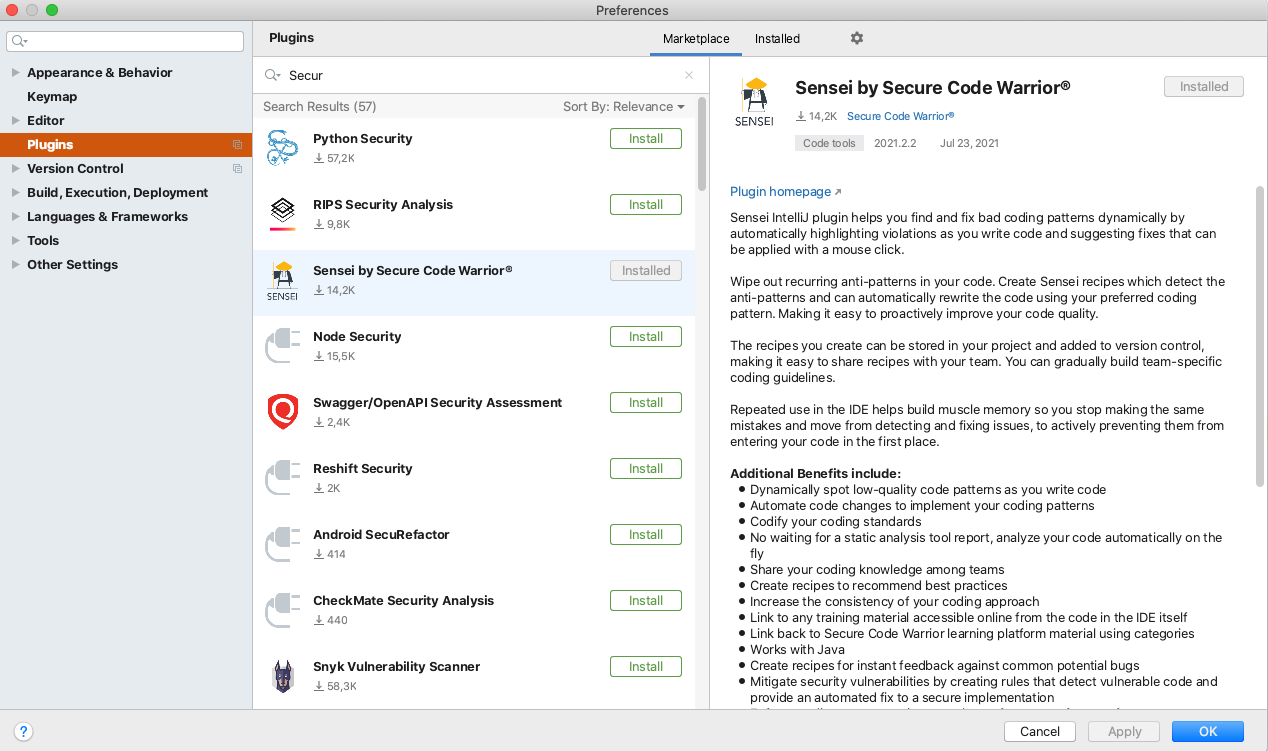
\includegraphics[width=\textwidth]{pluginsmenu.png}
  \includegraphics[width=\textwidth,page=2]{04-tools/figures/figures2.pdf}
  \caption[IntelliJ IDEA Plugins menu]{The Plugins menu in the IntelliJ IDEA allows developers to browse and easily install and uninstall extensions to their IDE.}
  \label{fig:pluginsmenu} 
\end{figure}

Sensei is available in the JetBrains Marketplace and can be installed through this Plugins menu.
Customized versions of Sensei can also be installed through this menu.
Such customized versions might be useful to disable certain features, or to automatically include certain rule sets.
To install customized versions, the Plugins menu needs to be configured to use additional plugin repositories, as shown in Figure~\ref{fig:pluginrepos}.
In this menu the developer needs to add a \gls{url} to locate the Sensei version that should be installed.
The customized version will then show up in the list of plugins in the regular menu.
This installation process is used in an experiment as described in Section~\ref{sec:experiment}.

\begin{figure}
  \centering
  %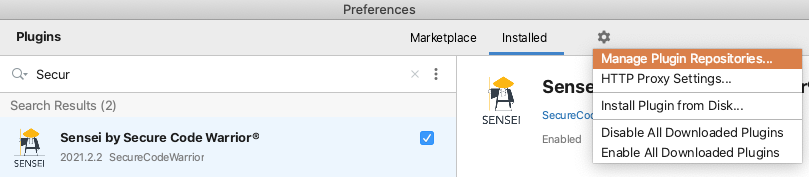
\includegraphics[width=\textwidth]{pluginrepos.png}
  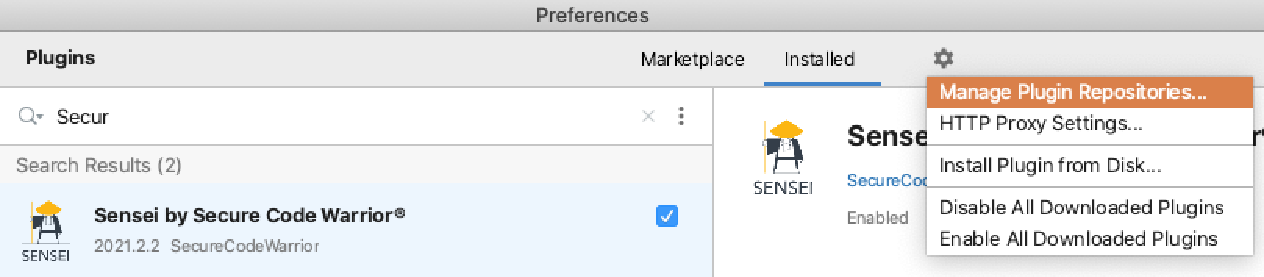
\includegraphics[width=\textwidth,page=1]{04-tools/figures/figures2.pdf}
  \caption[Adding plugin repositories to the Plugins menu]{The Plugins menu can be configured to add additional repositories of plugins, this allows us to install custom versions of the Sensei plugin that should not be distributed publicly.}
  \label{fig:pluginrepos} 
\end{figure}
\section{Recipes}

The \gls{api}-level rules that are enforced by Sensei are called recipes.
This name is chosen to emphasize the difference between Sensei and existing, traditional security tools, which often use rules to scan for vulnerabilities.
Recipes are also commonly used in the \gls{devops} movement, for example by the popular automation tool Chef~\footnote{\url{https://www.chef.io/}}.

\subsection{Creating recipes}
Customization and distribution of the recipes is a crucial feature for any successful tool supporting the paved path methodology.
If the recipes are easy to customize, Sensei can be more easily tuned to provide highly relevant and applicable feedback to the developer.
This customization should be scalable and hence not be a service provided by engineers or experts at \gls{scw}.
It should allow developers and security experts to effortlessly share project-specific or team-specific guidelines among each other.
For this reason, the recipe creation process should be easy and fast, and at the same time versatile. 

Our first approach allowed users to create new recipes through predefined recipe models.
A \gls{gui} was used to let the recipe-writer fill in a number of variables for this model.
A simple example of such a model is  the ``Replace method call model”.
Figure~\ref{fig:recipeedit2} shows a recipe being created to replace the \texttt{addCookie} method with a safe alternative from the \gls{owasp} \gls{esapi}, an open-source, web application security control library designed to make secure development easier~\cite{ESAPI}; the organization also provides some commonly used security guidelines.
The recipe-writer has to fill in some specifics about the method they want to be marked by Sensei, such as the package, class, and method names.
Then they can write one or more quick-fixes.
To create quick-fix, they have to write a quick-fix description and they have to define the code fragment that will be used to replace the original.
For the replacement code, they can reuse arguments, method names, and more from the original code by means of a template language.
In the field ``Rewrite to", the example quick-fix reuses the first argument of the original method call by using the template \texttt{arguments.0}. 

\begin{figure}
  \centering
  %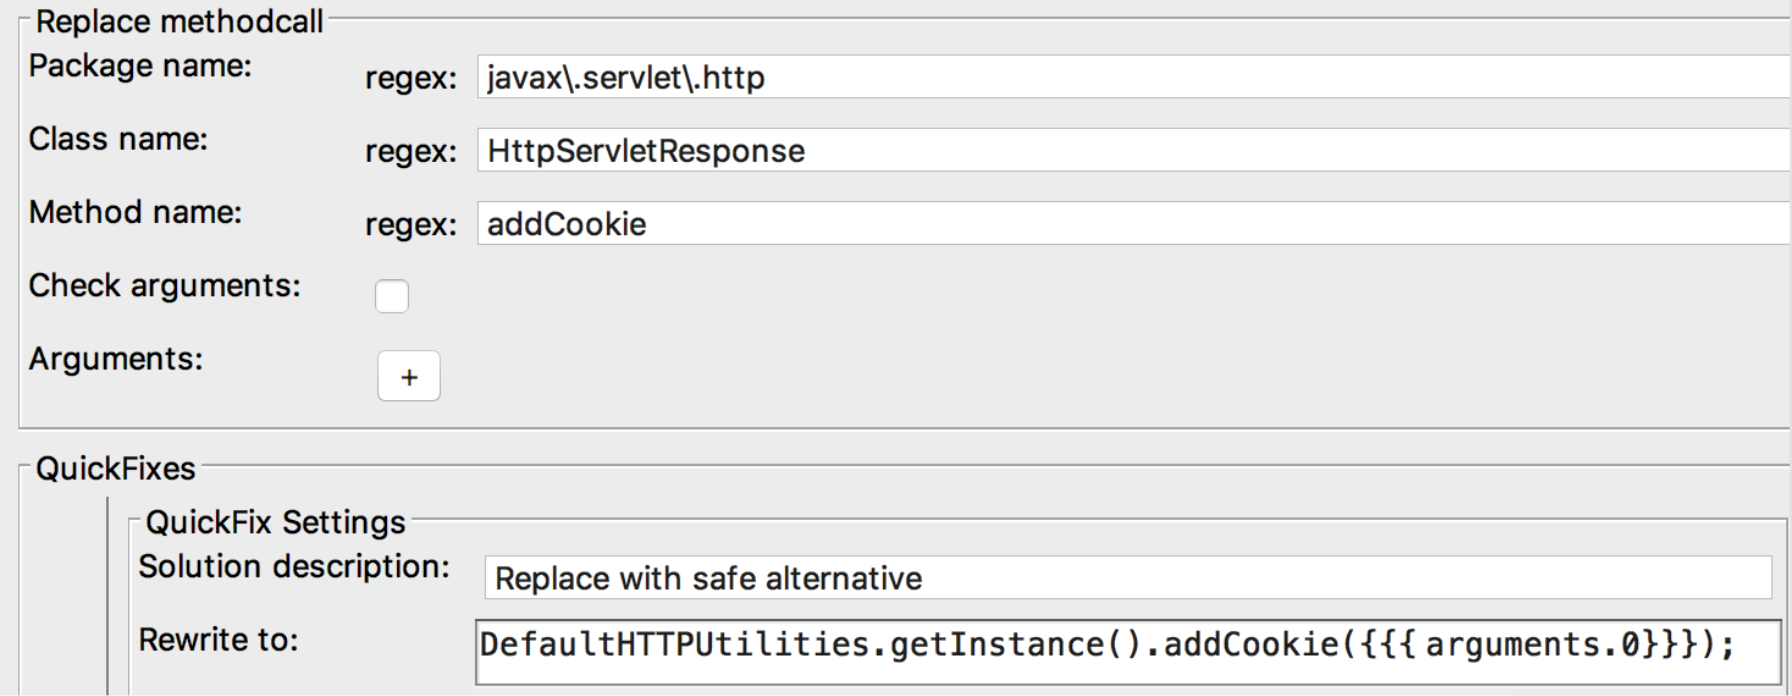
\includegraphics[width=\textwidth]{ruleedit2.png}
  \includegraphics[width=\textwidth,page=7]{04-tools/figures/figures2.pdf}
  \caption[Old model-based recipe editor]{The old recipe editor used a \gls{gui}. It required the recipe-writer to fill in a number of input fields to specify the behaviour of the recipe.}
  \label{fig:recipeedit2} 
\end{figure}

However, for more complex models the number of input fields grew rapidly to accommodate a plethora of corner cases, and so did the number of models for multiple scenarios.
As of now the old recipe editor has over 40 different models.
With this many models, it becomes overwhelming for recipe-writers that have to select a model to enforce their desired coding guideline.
The described model-based recipe creation process is not flexible and intuitive enough, so in the next iteration Nathan Desmet and I designed a new approach.

In this approach we split up the recipe in two parts: A trigger to identify the violation, plus an optional quick-fix to correct the vulnerability consistently according to company best practices.
Triggers are now specified by way of \gls{yaml}\footnote{\url{https://yaml.org/}} syntax, which provides more flexibility.
To develop this \gls{yaml} syntax, all existing Sensei rules were analyzed and grouped based on which elements in the code are incorrect and which transformations are required to fix them.
The resulting taxonomy of 10 bad code patterns is included in Appendix~\ref{app:patterns}.

Since this approach requires recipe-writers to learn the new syntax, we have provided some tools to assist them, in the form of a \gls{gui} that can be used to build the desired recipe from scratch.
In addition, the recipe editor is now more context-aware.
The recipe-writer can open a recipe creation wizard by pressing a key combination in the text editor in the \gls{ide} and selecting ``create new recipe".
This opens a context-aware menu depending on the position of the caret.
For example, if the caret was on a method call, the menu contains an option to create a new recipe that searches for similar method calls, as shown in Figure~\ref{fig:newrecipemethodcall}.

\begin{figure}[t]
  \centering
  %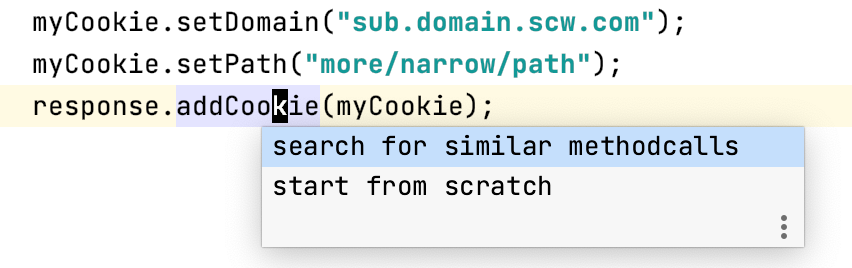
\includegraphics[width=0.8\textwidth]{rulewizard2.png}
  \includegraphics[width=0.8\textwidth,page=11]{04-tools/figures/figures2.pdf}
  \caption[Context-aware recipe creation menu]{The recipe creation menu is context aware, its options will change based on the caret position.}
  \label{fig:newrecipemethodcall} 
\end{figure}

When this context-aware option is chosen, the recipe creation wizard is opened and a recipe is automatically suggested from the available context.
To search for a methodcall, the information that can be pre-filled from context is the type and the name of the methodcall, as well as the number of arguments and each of their types.
The user can then adjust the recipe to reach the desired results through the \gls{yaml} code or the provided \gls{gui}.
This window also provides a preview panel, as shown in Figure~\ref{fig:recipewizard1}.
In this panel, the code file from which the recipe wizard was opened is shown, and the effects of the recipe being created are visualised, which allows for easy customization.

\begin{sidewaysfigure}
  \centering
  %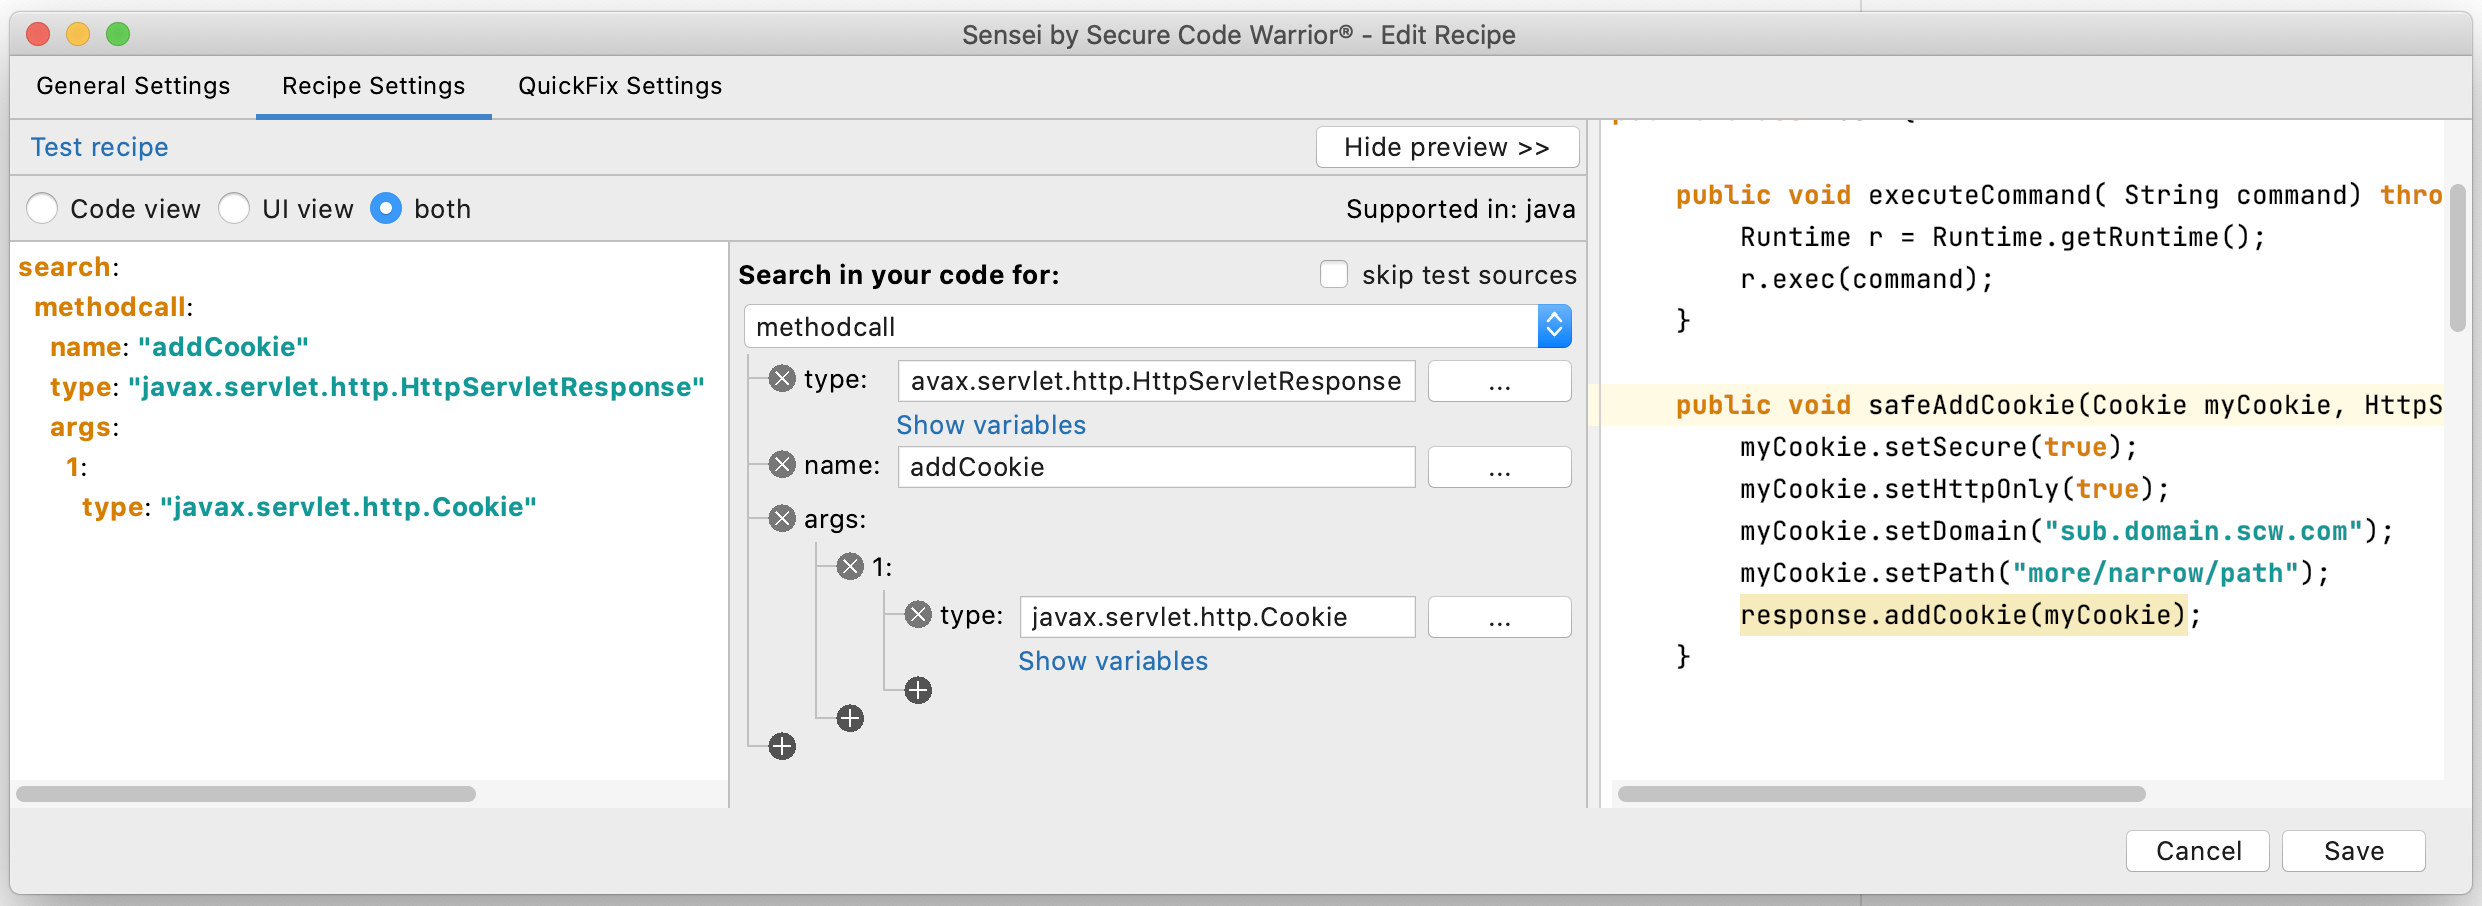
\includegraphics[width=\textwidth]{rulewizard1.png}
  \includegraphics[width=\textwidth,page=10]{04-tools/figures/figures2.pdf}
  \caption[Recipe created from context]{A recipe created through the ``search for similar methodcalls" option in the context-aware recipe creation menu will generate a \gls{yaml}-based recipe with details from the context of the caret position.}
  \label{fig:recipewizard1} 
\end{sidewaysfigure}

After creating a trigger, it is possible to create an optional quick-fix.
Here, the recipe-writer has to fill in the quick-fix description and the replacement code.
For the replacement code, they can make use of the same template language as in the first approach to reuse parts of the original code.
Below the input field, an overview is provided of the available parts of the original code, as shown in Figure~\ref{fig:createfix}.
Double clicking one of these options, adds its template to the fix.
The quick-fix creation window also offers a live preview in the lower right corner that highlights the changes that would be made to the original code (shown in the lower left corner) if the quick-fix is applied.

\begin{figure}
  \centering
  %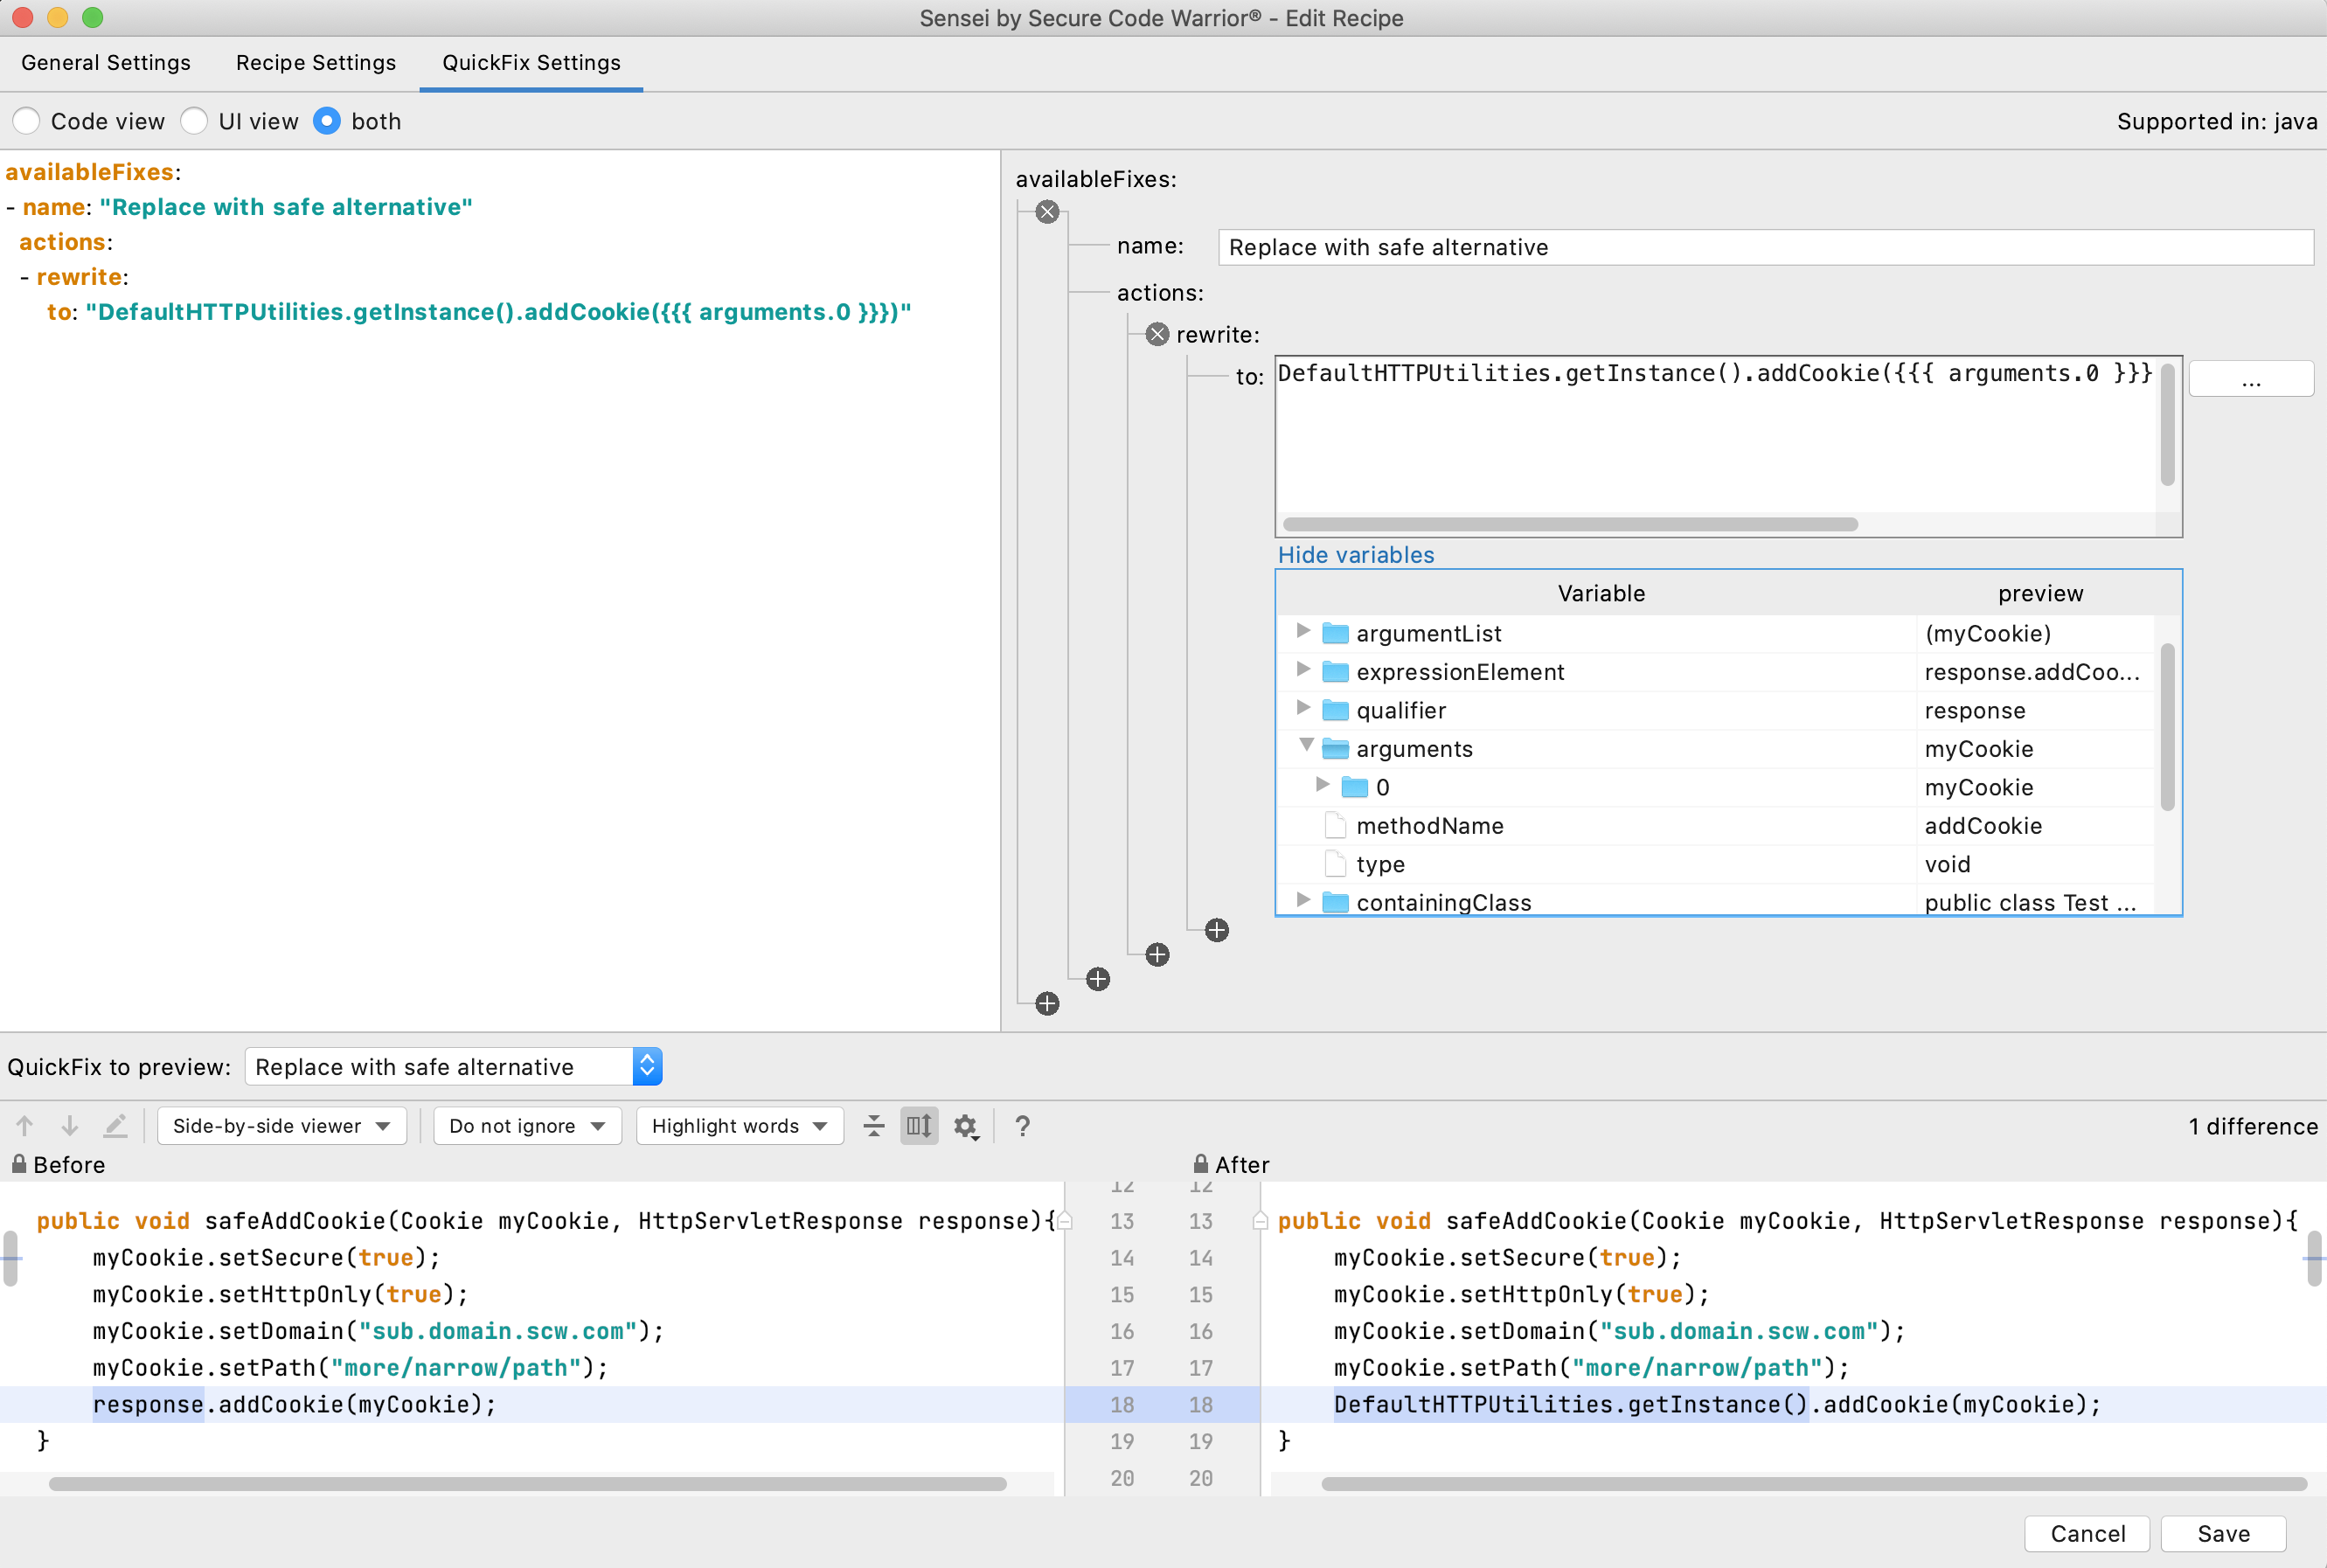
\includegraphics[width=\textwidth]{createfix.png}
  \includegraphics[width=\textwidth,page=5]{04-tools/figures/figures1.pdf}
  \caption[Fix creation window]{The fix creation window allows the recipe-writer to reuse parts of the original code.}
  \label{fig:createfix} 
\end{figure}

Finally, besides the trigger and the fix, there are also a number of general settings for the recipe that can be configured, as shown in Figure~\ref{fig:generalsettings}.
Some examples are the name, descriptions, the category of a related vulnerability, overriding recipes, and scopes.
All of these features are related to the usability of the developer and will be discussed in the following sections.

\begin{figure}
  \centering
  %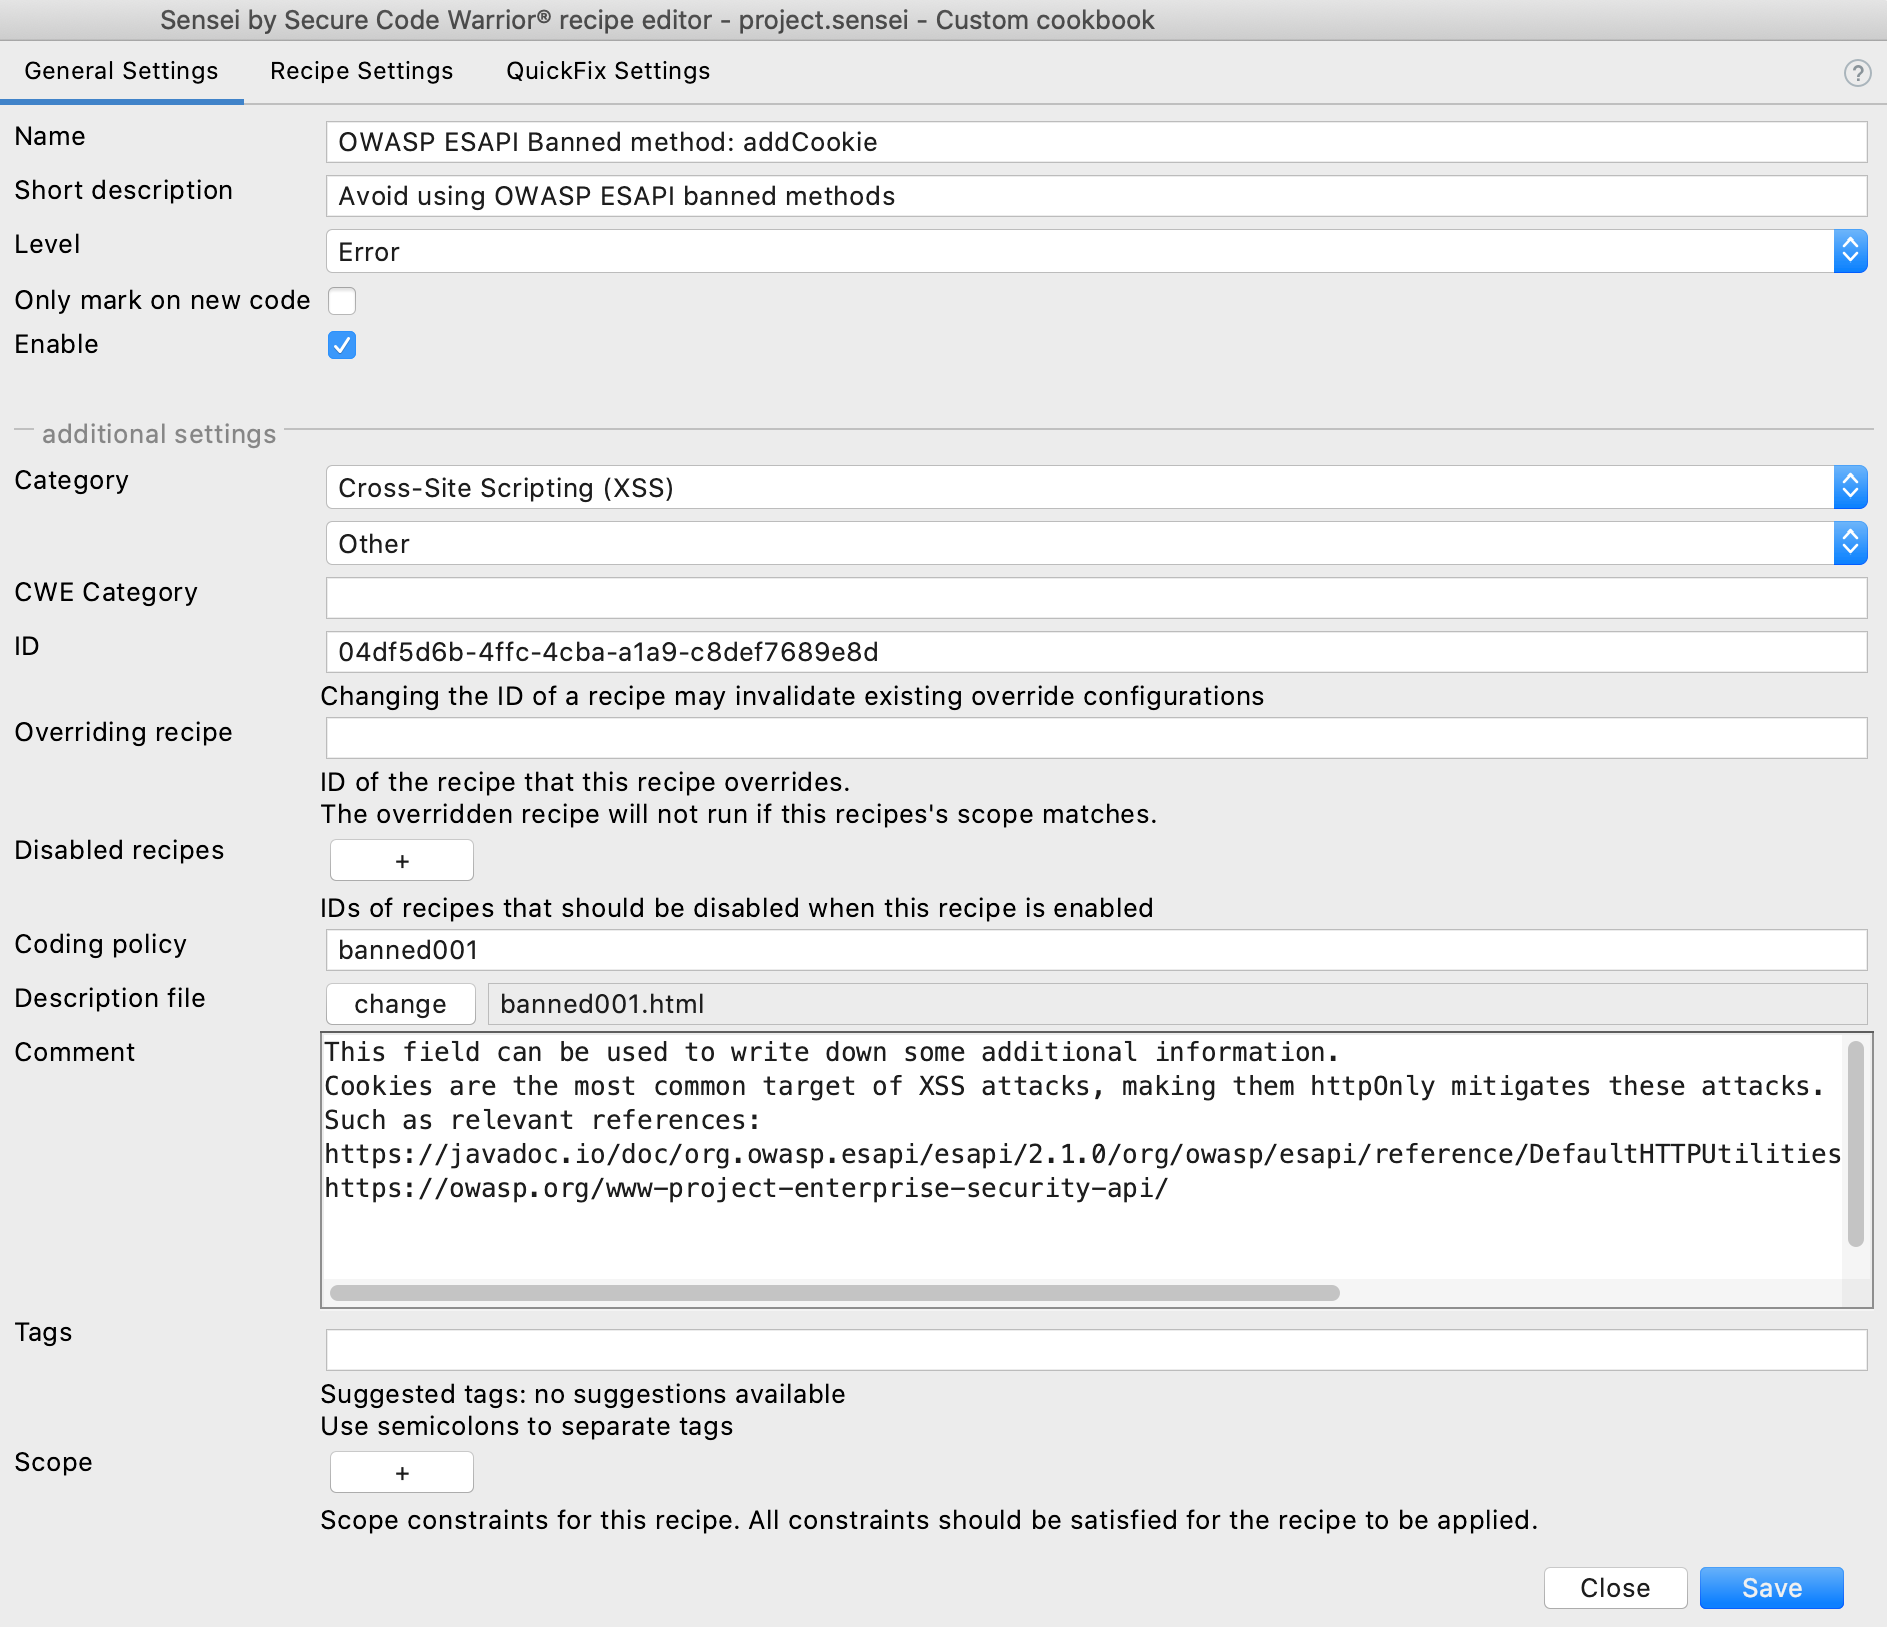
\includegraphics[width=\textwidth]{rulegeneral.png}
  \includegraphics[width=\textwidth,page=8]{04-tools/figures/figures2.pdf}
  \caption[General recipe settings]{Some additional settings are available in the recipe editor mostly related to usability of the developer.}
  \label{fig:generalsettings} 
\end{figure}

When creating recipes in-house, we have observed that the context-aware recipe wizard has greatly sped up the recipe creation process.
In practice, creating new recipes often starts from a bad code example, either when fixing a vulnerability or while reviewing the code of a colleague.
The recipe-writer can then simply open the recipe creation wizard from this example.
The live previews also greatly improve the usability, since before they were introduced, to create a finished recipe the recipe-writer was required to go back and forth several times to test the recipe in the \gls{ide} and adjust it in the recipe editor.



\subsection{Managing recipes}
\label{sec:manager}
%\todo[inline]{could you please explain how a developer would know where to consult for recipe sets, depending on which APIs are being used in a program? Bjorn: Mijn originele vraag is nog steeds geldig: Waarom denk je hier niet explicieter op te antwoorden? De vraag is volgens mij hoe developers de sets kunnen consulteren, hoe ze weten welke sets voor hen toepasbaar zijn. De vraag van de reviewer was niet hoe de regels tot stand komen.}
In the paved path methodology, guidelines can be put in place at the start of the project.
If not, at the very least, relevant guidelines should be created each time a new feature is going to be developed.
Together with those guidelines, Sensei recipes should be created as well.
The recipes, however, can also be used by the developers themselves, as a way to share knowledge.
When they develop new \glspl{api}, additionally to documentation, developers can also add Sensei recipes to the project that help their colleagues use these \glspl{api} as intended.

We also recommend to make Sensei recipes part of the remediation process when problems are found by security testing or reported through bug bounty programs.
It should be part of the process to create a recipe that prevents this same vulnerability from occurring in the future.
Currently, it is often the case that security experts run the security scans.
When problems are found, these experts guide the developers by providing them with informal, broadly applicable guidelines and checklists.
These instructions sometimes use security jargon that might not be clear to all developers, and even if they are understood, that does not guarantee the developer will be able to apply them in practice.
In the paved path methodology, security experts and developers should work together to create \gls{api}-level guidelines instead.
As part of this process, to communicate these guidelines to the rest of the team, Sensei recipes can be created as well.

For existing projects, we recommend companies to start with no recipes and use existing data on the security of their project as a starting point.
This could be the report of a penetration test, or results of vulnerability scans.
While resolving these issues in the code, developers and security experts can start building the first recipes.
Some clients of \gls{scw} have been hesitant to start with an empty security tool and, despite our recommendations to customize recipes for each project, still wish to receive starting recipes.
For this reason we have created small open-source sets of unopinionated recipes that can be used in all projects\footnote{\url{https://securecodewarrior.github.io/public-cookbooks/}}.
These recipes aid in correctly using the standard libraries of certain popular frameworks (e.g., Java 
\gls{ee}, Android \gls{sdk}, \gls{aws} \gls{sdk}).
This set can be used as inspiration and to get both security experts and developers accustomed to the tool, but usually it does not flag many issues.

Considering the different sources of recipes, developers can have recipes imposed by management and/or by the security team, as well as recipes distributed among the developers per team or project.
On top, there is the open-source recipes that can be used as a starting point when first using the tool.
To make the management of recipes easier, we group recipes into cookbooks.
Instead of distributing recipes one-by-one, this allows for grouping and distributing related recipes more easily. 

In order to manage these cookbooks in the \gls{ide}, a cookbook manager is provided, as shown in Figure~\ref{fig:cookbookmanager}.
Each cookbook is specified by a name and a location.
The developer can enable or disable any cookbook as well as edit recipes in some cookbooks.

\begin{figure}
  \centering
  %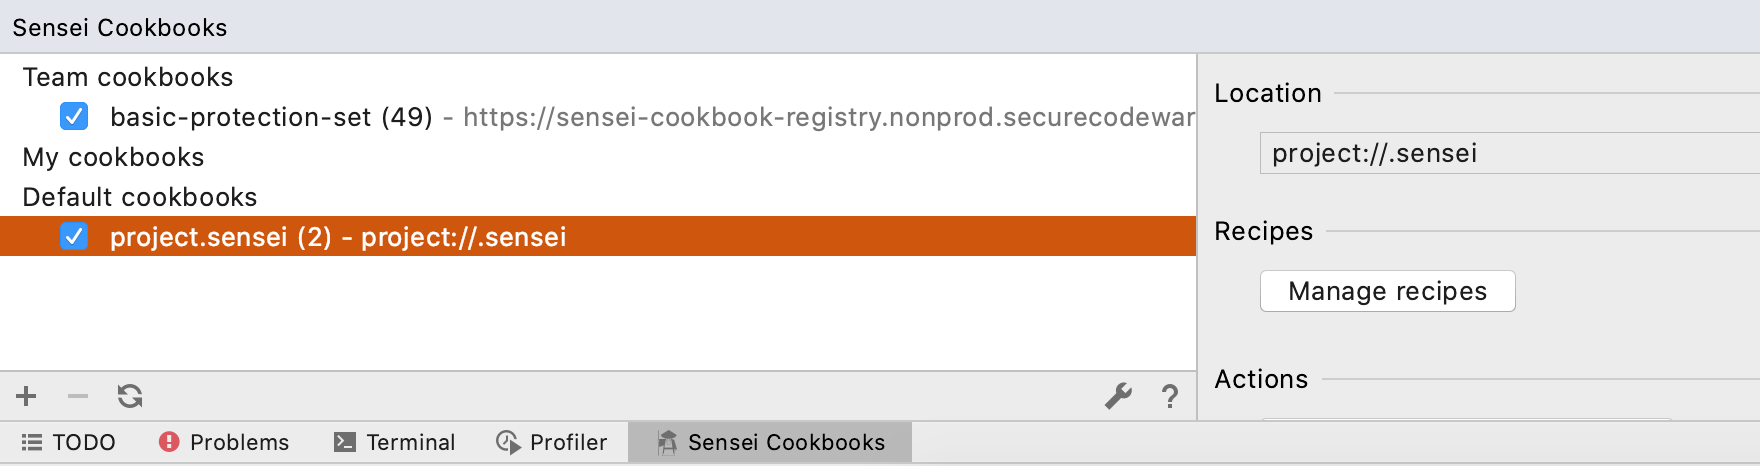
\includegraphics[width=\textwidth]{cookbookmanager.png}
  \includegraphics[width=\textwidth,page=3]{04-tools/figures/figures1.pdf}
  \caption[Cookbook manager]{The cookbook manager in this screenshot contains one remote team cookbook as well as one default cookbook stored in the project structure.}
  \label{fig:cookbookmanager} 
\end{figure}

Cookbooks can be stored locally or remotely.
Remote cookbooks are called team cookbooks and can be loaded from a github project (e.g., \texttt{git@gitserver:cookbooks|master|recipes}) or another remote server location (e.g., \texttt{https://remote.com/recipes.zip}).
Remote cookbooks are only recommended to distribute generally applicable cookbooks, since remote recipes are not editable by the developers and are instead read-only.
Any updates to the remote cookbooks are automatically pushed to all the developers.
Locally stored cookbooks are editable and can be specified by a local path (e.g., \texttt{/Users/dev/recipes}) for personal cookbooks or a path starting from the project root (by default \texttt{project://.sensei}) for default cookbooks for a project.
Local cookbooks are editable which means they can also be enabled on a recipe-by-recipe basis.
It is advised to store project specific recipes as part of the project.
This way, the recipes are always available, up-to-date with the code, and following the same flow as regular code (e.g., branch, review, merge).
When recipes follow the same flow as the code, new \glspl{api} and the recipes needed to use them properly can be added to the project and reviewed as a whole. 

The paved path methodology encourages customization of the recipes at project level.
Previous research and experience have shown that customization at at this level is the most successful.
This provides the needed flexibility to tailor the enforced coding guidelines to the code, but also ensures that the team has a joint approach to how the code for a project should be developed~\cite{sadowski2015tricorder}.
Individually customized recipes might lead to disagreements, while company-wide recipes might be too general to be easily applied.

It is possible for a recipe to be configured to disable other recipes, as shown in the general settings in Figure~\ref{fig:generalsettings}.
This feature can be used to improve remote, read-only recipes.
It is possible that such a recipe is not fully applicable to the project, e.g., because it requires too many manual adaptations.
It is then possible to create a replacement recipe that can be distributed to one team or project and disables the original recipe when it is active.
To facilitate this, an option in the quick-fix menu is added to copy remote recipes to a local cookbook, as shown in Figure~\ref{fig:copyrecipe}.
This option can easily be hidden in the settings.
The clone recipe window, shown in Figure~\ref{fig:clonewindow}, provides an option to automatically disable the original recipe it is copied from.
When a remote recipe is disabled or replaced, the author of this recipe should be notified.
It is possible that it is a generally applicable improvement and the recipe can be updated accordingly for other teams or projects that use it in a remote cookbook.
An additional quick-fix option will be added in the future to disable a recipe.

\begin{figure}
  \centering
  %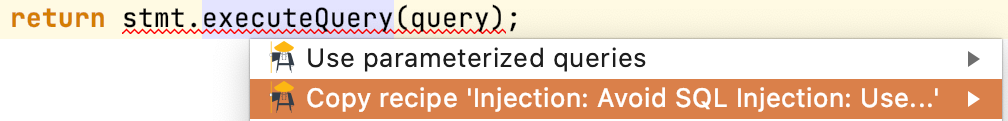
\includegraphics[width=\textwidth]{copyrecipe.png}
  \includegraphics[width=0.9\textwidth,page=4]{04-tools/figures/figures1.pdf}
  \caption[Copy recipe option in the quick-fix menu]{For remote recipes, the quick-fix menu offers a ``Copy recipe" option.}
  \label{fig:copyrecipe} 
\end{figure}

\begin{figure}
  \centering
  %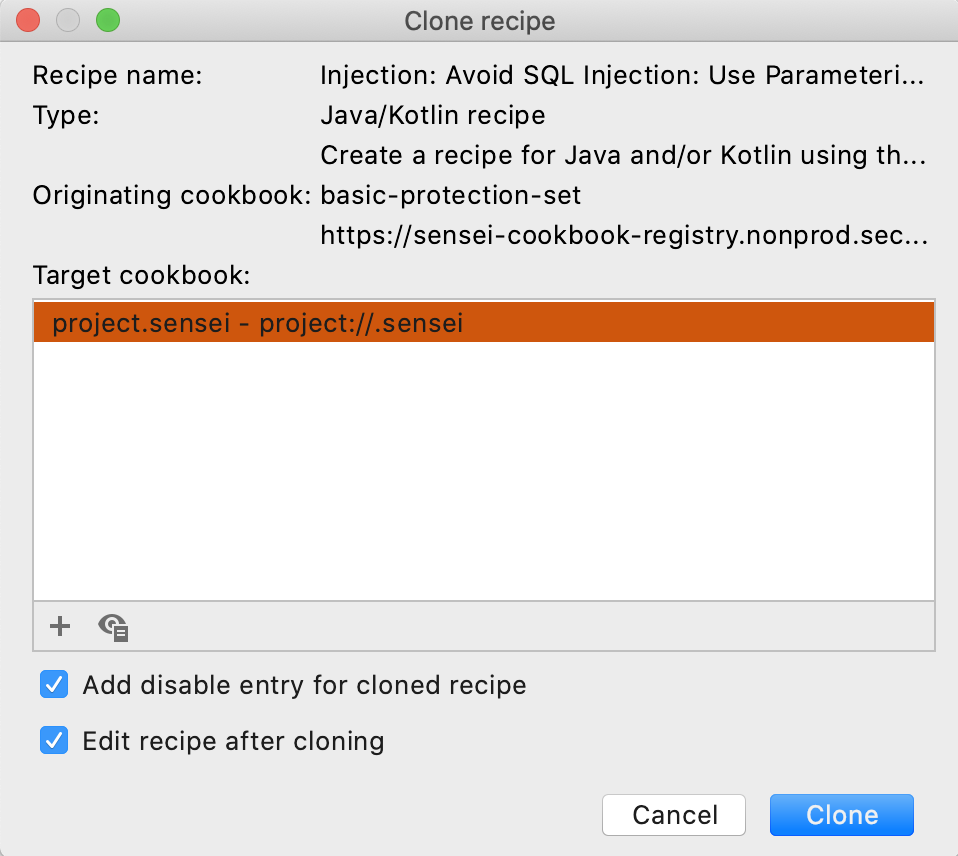
\includegraphics[width=0.75\textwidth]{clonerecipe.png}
  \includegraphics[width=0.75\textwidth,page=2]{04-tools/figures/figures1.pdf}
  \caption[Clone recipe window]{The clone recipe window allows the recipe-writer to configure the new recipe to disable the recipe it is copied from.}
  \label{fig:clonewindow} 
\end{figure}

The discussed features to disable recipes have been designed to improve the usability of the tool for developers.
They are in line with the philosophy that developers' productivity benefits from their ability to customize their development environment to their preferences, and to give them a significant amount of freedom in that regard.
In that philosophy, it is preferable to have developers disable some recipes rather then uninstalling or neglecting the tool completely.
Importantly, this does not necessarily result in guideline violations slipping below the radar, since security and management can still have these recipes, as well as complimentary tools, enabled in later phases of the \gls{sdlc}.

\subsection{Verifying recipes}
To inspect the code against a number of recipes, our tool reuses the \gls{ide} syntax checking features.
When a developer writes new code, the \gls{ide} rebuilds the \gls{ast} and computes the changes compared to the previous version.
A limited \gls{ast} of the changes, containing the necessary symbol information, is then passed on, allowing tools to only analyze the changes.
On this \gls{ast}, a combination of specialized light-weight versions of existing analysis techniques is used such as taint analysis, data flow analysis, and control flow analysis to verify the recipes in real time.

\subsection{Explaining recipes}
\label{sec:information}
In order to mark violated guidelines, our plugin makes use of existing \gls{ide} features to flag coding mistakes.
In most \glspl{ide} the code markings by default have three levels of severity: \emph{error}, \emph{warning}, and \emph{information}.
We recommend to mark coding guideline violations as errors.
Traditional error-level markings are usually immediately addressed by the developer, while warning-level markings are more frequently ignored~\cite{whitney2018embedding}.
This is the case because error-level warnings in an \gls{ide} typically indicate a problem in the code that will result in a compilation failure.
Currently error markings by our tool still allow successful compilation of a project, but several clients have requested for the markings to result in compilation failures, equivalent to errors marked by the \gls{ide} itself.
This is not surprising, as it is in line with the default behavior of popular \glspl{ide} such as Visual Studio.
For example, when Visual Studio's C compiler compiles code that uses the insecure \texttt{sprintf} function, it throws a compilation error warning the developer that the function may be unsafe.

An example marking can be seen in Figure~\ref{fig:publicactivity}, where the opening \texttt{<activity>} tag in \gls{xml} code is marked as an error.
This marking makes the code fragment stand out and attracts the developer's attention.
In the example, the Android activity is configured as a public activity by setting the \texttt{exported} attribute to \texttt{true} but not configuring an intent filter.
In \gls{xml} code, like in this example, it is advised to only mark the opening tag, and not the entire \gls{xml} tag and its content.
This would overwhelm the developer, and it would not be clear which part of the code is lacking. 

\begin{figure}
  \centering
  %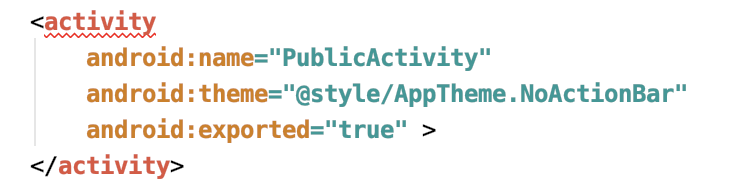
\includegraphics[width=.75\linewidth]{publicactivity.png}
  \includegraphics[width=0.75\textwidth,page=3]{04-tools/figures/figures2.pdf}
  \caption[Error marking on an XML opening tag.]{\Gls{xml} recipes can be configured to mark the opening tag only (shown in the figure), the opening tag and the closing tag, or both tags and their entire content.}
  \label{fig:publicactivity} 
\end{figure}

Permanent markings, that remind developers of security implications of their decisions, should be marked as information.
To continue on the example of private and public activities, in the code file that implements the activity, we mark the class definition at the information level.
Hovering over the marking informs the developer whether the activity is configured as public or private, and provides a direct link to detailed information about the security implications.
This marking is shown in Figure~\ref{fig:infomarking}.
Note how the markings are clearly visible and noticeable, but at the same time non-intrusive to developers already used to their \gls{ide} flagging code fragments.

\begin{figure}
  \centering
  %
\includegraphics[width=0.80\linewidth]{infomarking2.png}
  \includegraphics[width=0.8\textwidth,page=10]{04-tools/figures/figures1.pdf}
  \caption[Marking at the information error level]{The information error level marking is clearly visible but at the same time non-intrusive, as this is a permanent marking that can not be resolved.}
  \label{fig:infomarking} 
\end{figure}

The marking of code is accompanied by three descriptions.
The information in these descriptions is important to ensure the continued use of the tool~\cite{whitney2018embedding,layman2007toward}.
Developers build trust with analysis tools, and this trust is quickly lost if they do not understand the tool’s output~\cite{bessey2010few}.
The first description is the short error description, i.e., the text that appears when the developer hovers their mouse pointer over the marked code.
It should be just one line.
The purpose of this description is to attract attention, inform the developer that something should be addressed, not to explain how to address it.

We have learned through user feedback that it is most effective to attract the user's attention by starting with the “why”~\cite{RSAvideo}, the reason the code is marked and should be addressed.
In the past the short description used to indicate the possible vulnerability class, for example “Could lead to SQL injection”. 
We believed that starting with the potential consequences, makes the developers realize the severity of their mistake and encourages them to immediately address it.
However, as explained in Section~\ref{sec:communication}, security jargon should be avoided when communicating to developers.
The feedback in all of the descriptions should be targeted at developers, and hence the focus should be on the guidelines that were put in place, on the paved path.
A better short description is hence, “Violates a guideline on data retrieval”, as depicted in Figure~\ref{fig:shortdescription}.

\begin{figure}
  \centering
  %\includegraphics[width=\linewidth]{shortdescription2.png}
  \includegraphics[width=\textwidth,page=14]{04-tools/figures/figures2.pdf}
  \caption[Short description of a recipe]{The short description of a recipe is visible when hovering over a marking. It should attract the developers attention but avoid security jargon. Instead, the developer can be reminded of guidelines that are in place.}
  \label{fig:shortdescription} 
\end{figure}

Next to the short description a “read more” link is created by the \gls{ide} for the interested developer.
Upon clicking this link, a pop-up is opened to show a more elaborate \gls{html} page.
This is the second description.
Figure~\ref{fig:fulldescription} shows an example.
This description is called the full coding guideline.
The page starts with a short abstract, stating in one sentence what should be done, such as “Secure coding practices prescribe that queries need to be parameterized”.
The page's next section presents in detail what it means to use parameterized queries and gives an overview of the approved \gls{api} methods.
Small code examples are included as well, since previous research has shown examples are the fastest way for developers to understand a problem~\cite{whitney2018embedding}.
The goal of this description is after all to help developers find out quickly how to comply to the coding guideline without spending much time or effort.
This is crucial for a security tool to feel well integrated into developer workflows.
The last section of the description contains a list of possible consequences when the developer fails to address this issue.
There is no mention of vulnerabilities or exploits until this point.
Each item in the list contains a link to the \gls{scw} training platform to learn more about the vulnerabilities and how they are exploited.
This way an interested developer (with too much time on their hands?) can still easily find the necessary information to learn the details of each vulnerability and the possible attacks.
Following this training would require a context switch and would likely hurt developer productivity.
In the future the integration between the \gls{scw} training platform and the Sensei \gls{ide} plugin can be improved as described in the perspectives in Section~\ref{sec:its-integration}.

\begin{figure}
  \centering
  %\includegraphics[width=\textwidth]{guideline.png}
  \includegraphics[width=\textwidth,page=7]{04-tools/figures/figures1.pdf}
  \caption[Example of the full coding guideline.]{The full coding guideline is a more elaborate \gls{html} page that explains the guideline in more detail and provides code examples.}
  \label{fig:fulldescription}
\end{figure}

The third description is visible to the developer when they press the \gls{ide}’s key combination to start resolving the issue.
A drop down menu appears, containing the possible quick-fixes' descriptions.
%A "copy recipe" option is available as well, and for local recipes there is also additionally an "edit recipe" option, both of these can be disabled in the Sensei settings.
IntelliJ also provides options to disable inspections locally or globally. Figure~\ref{fig:qfdescription} shows an example.
In this menu we provide a very short description of the actions that will be performed when this code transformation is chosen, such as “Use parameterized queries”.
A brief yet descriptive quick-fix description allows developers to decide quickly whether the fix is appropriate for them.
If the effects of applying the quick-fix are well understood, the developer will trust the tool and apply the fixes more often.
Sometimes the developer needs to choose between different possible solutions.
However, it is advised to keep the number of fixes as low as possible, as to not complicate the issue unnecessarily.

\begin{figure}[t]
  \centering
  %\includegraphics[width=\textwidth]{quickfixmenu.png}
  \includegraphics[width=\textwidth,page=5]{04-tools/figures/figures2.pdf}
  \caption[Example of the quick-fix description.]{The quick-fix description briefly describes the actions that will be performed when each option is chosen. IntelliJ also offers a feature to suppress markings of any inspection (Sensei or otherwise).}
  \label{fig:qfdescription} 
\end{figure}

\section{Recipe features}
\label{sec:features}

Over time, several advanced features in the recipes have been developed following user feedback.
In this section, I explain the problems they tackle and provide code examples for each one.

\subsection{Lowering effective false positives}
\label{sec:efp}
It is important to choose the right error level for the developer to pay attention to the markings, but also not to overwhelm them with markings to the point that they start to ignore them.
Since the recipes can be created by anyone in the team, they should not be too obtrusive.
To a recipe writer, a false positive is an incorrect marking of code that is not violating a coding guideline.
However, to a developer, a false positive is any code marking that they do not intend to fix and ignore instead~\cite{ayewah2007evaluating}.
A false positive from the perspective of the developer is also called an \gls{efp}~\cite{sadowski2015tricorder}.
To ensure the usability of the tool, the \gls{efp} rate should be sufficiently low~\cite{sadowski2015tricorder,johnson2013don}.

To demonstrate \glspl{efp} we take a look at \gls{os} Command injection.
One of the \glspl{api} that is banned in the \gls{owasp} \gls{esapi} guidelines is \texttt{Runtime.exec}.
This \gls{api} is used to execute \gls{os} commands in Java programs.
When user input is added to this command, \gls{os} command injection is possible and the attacker can gain access to the underlying \gls{os}.
Using this information it is possible to create a recipe that marks all uses of the \texttt{Runtime.exec} method.
While this is a good coding guideline, a security conscious developer recognizes that the method needs user input before it can lead to \gls{os} command injection.
In rare occasions an \gls{os} command might be necessary for functionality and perfectly valid and secure.
For example, launching another software product can be done securely as long as the command is hard-coded.
An example of insecure usage of the \texttt{Runtime.exec} method can be found in Listing~\ref{lst:oscommand1}, examples of secure usage in Listings~\ref{lst:oscommand2}~and~\ref{lst:oscommand3}.
The two secure examples are still violations of the above coding guideline, and they get flagged.
An experienced developer has no intent to fix them, meaning they are two cases of \glspl{efp}.
Notice how this \gls{efp} depends on the knowledge and skill of the developer, meaning that it might be beneficial to adjust the feedback of the tool for individual developers, as explained in the perspectives in Section~\ref{sec:sensei-perspectives}.
%A similar example leading to \glspl{efp} is when hard-coded \gls{sql} queries are created without using parameterized queries.
%These queries would violate a guideline enforcing parameterized queries, but they would not be insecure, not even when this function is reused from a different context in the future.

In order to keep the \gls{efp} rate sufficiently low we have introduced the concept of \emph{trusted input}.
Hard-coded input is automatically trusted, since a user can not influence it, and hence it can not lead to a vulnerability.
However, function parameters and variables from other origins are considered untrusted by default.
This is still in line with the philosophy to protect methods from future use, where we want to flag violations that can one day lead to vulnerabilities.
The requirement in recipes of untrusted input can be added to arguments, this can be done using the \gls{yaml} syntax or by using the \gls{gui} as shown in Figure~\ref{fig:recipegui}. 
The next step is to define trusted sources. This also avoids the \gls{efp} in Listing~\ref{lst:oscommand3}. The resulting recipe can be seen in Listing~\ref{lst:yamlrecipe}.

\begin{minipage}[t]{0.9\linewidth}
%\vspace{-0.4 cm}
\begin{lstlisting}[language={Java},caption={if the \texttt{command} variable contains unsanitized user input, this function is vulnerable to \gls{os} command injection.},label={lst:oscommand1},abovecaptionskip=-0.0pt,xleftmargin=15pt]
public void executeCommand(String command){
    Runtime r = Runtime.getRuntime();
    r.exec(command);
}
\end{lstlisting}
%\vspace{-0.3cm}
\begin{lstlisting}[language={Java},caption={Using a hard-coded command avoids the possibility that the variable will ever contain unsanitized user input.},label={lst:oscommand2},abovecaptionskip=-0.0pt,xleftmargin=15pt]
public void executeCommand(){
    Runtime r = Runtime.getRuntime();
    r.exec("explorer.exe");
}
\end{lstlisting}

\begin{lstlisting}[language={Java},caption={This code fragment is secure if the \texttt{getSafeCommand} method can be trusted to never return variables containing unsanitized user input.},label={lst:oscommand3},abovecaptionskip=-0.0pt,xleftmargin=15pt]
public void executeCommand(){
    Runtime r = Runtime.getRuntime();
    String command = getSafeCommand();
    r.exec(command);
}
\end{lstlisting}

\begin{lstlisting}[language={yaml},caption={This recipe trigger requires the argument of an \texttt{exec} methodcall to contain untrusted input before it will mark the methodcall. It also specifies the methodcall \texttt{getSafeCommand} as a trusted source of input.},label={lst:yamlrecipe},xleftmargin=15pt]
search:
  methodcall:
    name: "exec"
    type: "java.lang.Runtime"
    args:
      1:
        type: "java.lang.String"
        containsUntrustedInput: true
        trustedSources:
        - methodcall:
            name: "getSafeCommand"
\end{lstlisting}
\end{minipage}
%\vspace{-.3cm}

\begin{figure}[t]
  \centering
  %\includegraphics[width=\textwidth]{rulegui2.png}
  \includegraphics[width=\textwidth,page=9]{04-tools/figures/figures2.pdf}
  \caption[\Gls{gui} to add the requirement of untrusted input.]{It is possible to add requirements like untrusted input or an in-clause through the \gls{gui}.}
  \label{fig:recipegui}
\end{figure}

Another way to allow recipe writers to create more targeted recipes and to keep the \gls{efp} rate low, is to provide \emph{trigger scopes}.
Trigger scopes can be added by using the \texttt{in} keyword in the \gls{yaml} syntax, or by using the \gls{gui} as shown in Figure~\ref{fig:recipegui}.
The in-clause can define restraints on the context.
This makes it possible to create a recipe that prevents the usage of \texttt{Runtime.exec} except in a class with name \texttt{AppLauncher}.
Scopes like this can also help with performance, i.e., meeting the real-time checking requirement, since recipes that are out of scope can be skipped during analysis.

In the old editor, rather than \emph{trigger} scopes, \emph{recipe} scopes were a property of the entire recipe.
They were added by selecting the type of scope and filling in some fields.
By migrating these scopes to the \gls{yaml} syntax, the scoping of recipes becomes much more flexible.
The recipe scopes that can be migrated to trigger scopes are the class scope, method scope, file scope, Android context scope, and Android build property scope.
Descriptions of these scopes can be found in Appendix~\ref{app:recipe-scopes}.

There are two more recipe scopes, for which migration to trigger scopes is not useful.
The \emph{project scope} allows us to enable or disable recipes based on the name of the project.
This is useful when different cookbooks are required for each project in a company.
This scope is no longer needed since we now allow cookbooks to be stored in the project, which is a lot more convenient then adding a scope to each recipe separately.
The \emph{library scope} can be used to enable recipes based on the presence of a library.
This way we can disable a recipe if the fix uses a library that is not used in the project.
Since this scope is created for the fix of the recipe and not the trigger, it cannot be added to the \gls{yaml} syntax and remains a property of the entire recipe.
In the future it could be useful to add scopes to quick-fixes, so that a recipe can provide different fixes depending on the presence of a library.

\subsection{Support for libraries}
Often quick-fixes are small code changes, such as adding a preceding method call or changing a parameter, but sometimes they involve more elaborate pieces of code.
An example for this is adding a cookie to a \gls{http} request.
Before adding the cookie, it needs to be properly configured.
Insecure and secure code examples are shown in Listings~\ref{lst:cookie1} and~\ref{lst:cookie2}, respectively.

\begin{lstlisting}[float,language={Java},caption={This cookie is not configured before it is added to the response, as a result this code fragment is insecure.}, float,label={lst:cookie1},abovecaptionskip=-0.0pt]
Cookie myCookie = new Cookie("secure", "success");
response.addCookie(myCookie);
\end{lstlisting}

\begin{lstlisting}[language={Java},caption={Several configuration options are added to narrow the scope that the cookie can be used, and to ensure it is not sent over plaintext.}, float,label={lst:cookie2},abovecaptionskip=-0.0pt]
Cookie myCookie = new Cookie("secure", "success");
myCookie.setSecure(true);
myCookie.setHttpOnly(true);
myCookie.setDomain("sub.domain.scw.com");
myCookie.setPath("more/narrow/path");
response.addCookie(myCookie);
\end{lstlisting}

If this fix is applied at multiple locations in a project, it can result in code bloat.
It might then be better for the company to provide a method that replaces the original \texttt{addCookie} method.
In this method the cookies can be first configured properly before calling the original \texttt{addCookie} method.
Such replacement wrapper methodcall is shown in Listing~\ref{lst:cookie3}.
The new guideline for cookies is then to replace the \texttt{addCookie} method with the \texttt{safeAddCookie}, as shown in Listing~\ref{lst:cookie4}.
The creation of such a wrapper library is strongly recommended by the paved path methodology, as the resulting guidelines are very easy to understand by developers.
At the same time any security bugs are confined to the \textit{implementation} of the wrapper library, and no new bugs can be introduced by \textit{using} the wrapper library. This makes the job of the security team easier as well.

\begin{lstlisting}[language={Java},caption={A wrapper library can be created to avoid code reuse and to improve clarity of the guidelines for the developer.}, float,label={lst:cookie3},abovecaptionskip=-0.0pt] 
public void safeAddCookie(Cookie myCookie, HttpServletResponse response){
    myCookie.setSecure(true);
    myCookie.setHttpOnly(true);
    myCookie.setDomain("sub.domain.scw.com");
    myCookie.setPath("more/narrow/path");
    response.addCookie(myCookie);
}
\end{lstlisting}

\begin{lstlisting}[language={Java},caption={Migrating to the wrapper library consists of replacing the original methodcall with one from the library.},float,label={lst:cookie4},abovecaptionskip=-0.0pt]
Cookie myCookie = new Cookie("secure", "success");
safeAddCookie(myCookie, response);
\end{lstlisting}

The first example, where the cookie is configured properly, is a \emph{library usage recipe}.
This type of recipe provides guidance on using a library correctly.
The trigger of the recipe is on \glspl{api} from the library.
Code fragments are refactored without involving additional libraries, only libraries that are also used in the trigger.

The second example, where the insecure code is replaced with \gls{api} calls from a different library, is a \emph{library adoption recipe}.
Instead of providing guidance on the correct usage of the \glspl{api}, such recipes promote the adoption of a new library.
This type of recipe has a trigger in one library but their fix uses a different library.

As a proof of concept for library adoption recipes, support has been developed for the \gls{owasp} \gls{esapi} library.
Among others, the \gls{owasp} \gls{esapi} contains replacement methods for commonly used insecure \gls{jdk} methods, the so-called \gls{owasp} \gls{esapi} banned \glspl{api}\footnote{\url{https://www.owasp.org/index.php/ESAPI\_Secure\_Coding\_Guideline}}.
To support the \gls{owasp} \gls{esapi} in companies that adapt it, a recipe set was created to enforce the replacement of the banned \glspl{api} with their alternatives from the \gls{owasp} \gls{esapi}.
Feedback from these companies showed that this set of library adoption recipes was intuitive and easy to use for developers.
Importantly, it increased the speed of the library's adoption.

Library usage recipes are generally applicable to codebases because the trigger and fix of these recipes use \glspl{api} from the same library, thus ensuring that the recipes never mark any code when the fix is unavailable.
The trigger and fix for library adoption recipes depend on different libraries.
This implies that an applied quick-fix can result in the use of unavailable \glspl{api}. 

Library scopes can be used for this purpose.
When the library used in the quick-fix serves as a scope of a recipe, it will not mark any code if the library is unavailable.

\subsection{Support for detecting design flaws}
As discussed before, coding guidelines are enforced through mostly local analyses.
This allows Sensei to intervene earlier in the development process and makes it possible to perform the analyses in real time while the developer is typing.
For this reason the focus of the approach is mostly on implementation bugs.
Detecting design flaws in the application code (rather than in the \glspl{api} it relies on) is typically much harder.
Still, we have learned that various flaws can be tackled through the use of configuration files and the previously described trigger and recipe scopes.

An example of a flaw that is difficult to detect with local analyses is excessive security logging.
It is crucial to log important security events, but too much logging can make it difficult or impossible to locate certain events.
While enforcing guidelines can help with logging securely (e.g., not logging sensitive data, not logging unsanitized input, logging in proper format) it is difficult to monitor the frequency of the logging through local analyses.
Other examples are the use of transport layer security, or whether authorization is needed or not.

One scenario that, to the contrary, enables us to detect some design flaws, is when popular frameworks are used to handle security features.
For example, enforcing the use of transport layer security in an Android app is as simple as adding a line to the Android manifest about clear text traffic.
This can be seen in Listing~\ref{lst:manifest}, line 3.

\begin{lstlisting}[language={XML},caption={When the attribute \texttt{usesCleartextTraffic} is added to the Android manifest with value \texttt{false}, the Android \gls{os} will ensure that transport layer security is used for the communication with this application.},float,label={lst:manifest},abovecaptionskip=-0.5pt]
<application
     android:label="@string/app_name"
     android:usesCleartextTraffic="false">
\end{lstlisting}

Another example is the use of encryption.
It is trivial to detect if a deprecated encryption algorithm is used by means of a known \gls{api}, but it is much harder to detect the absence of encryption through local analyses.
One interesting class of mistakes that we observed was developers XOR’ing data, or encoding data, rather than encrypting it.
As a solution, a coding guideline can be created that requires functions whose name contains “encrypt” to perform encryption through some of their approved \gls{api} methods.
If such a function \emph{only} performs encoding or XOR operations, it implies that the required \gls{api} calls are missing.
In that case the tool suggests quick-fixes that insert the necessary \gls{api} calls.
These quick-fixes are only partial fixes: They inject code that invokes encryption routines on an unspecified string or byte array.
It is then still up to the developer to remove the XOR operations and fill in the correct string or array identifier.
This emphasizes again why it is beneficial to provide fixes in the \gls{ide} during development time.
When this recipe is used during the development of a new method, the developer starts by creating a function declaration.
When a function exists with ``encrypt" in the name and an empty body, this is marked, as the required \gls{api} calls are missing.
The fix then inserts the required \gls{api} calls, leading to comfortable and intuitive security help for the developer.
This recipe is a good example to demonstrate the paved path methodology.
It guides the developer along a predetermined path laid out for them to implement encryption securely.

We have also improved context-awareness to detect flaws by adding more recipe scopes.
One such example is the Android \emph{context scope}.
As explained earlier, in the Android manifest a developer can configure capabilities of components such as activities and broadcast receivers regarding their communication towards the \gls{os}.
They can listen to any other application, only to authorized applications, or only to the own application.
The Android context scope allows us to enable recipes based on the configuration of the relevant component, so that we can enforce different recipes for different levels of exposure.
Such a recipe can allow communication of sensitive information between classes that are configured as private components, but not between other classes.

\subsection{Testing recipes}
%\todo[inline]{Add example of indexing of arguments and quickfixes}
Testing custom recipes is a challenge.
When new recipes are created, the recipe writers first have to test the behaviour of the recipe manually.
They develop a few code fragments they expect to be marked, as well as some that should not be marked by the recipe.
They then apply the transformations and manually inspect the resulting changes.
The recipe wizard helps speed up these tasks by providing preview panels during recipe creation.
A recipe writer at a company, however, cannot be asked to perform the manual checks again every time they install updates to our plugin (including its underlying analyses) or to the \gls{ide} itself.
Such updates always risk altering the outcome of a recipe.
Instead automated unit testing is needed.

The plugin developer has sufficient capabilities to automate unit tests to verify the behavior of the analyses.
To do this they also create a few demo recipes and test the behavior of these recipes.
Since they have access to the code of the plugin, they can simply write unit tests and (directly) call internal plugin and exported \gls{ide} methods to test the markings and transformations and to compare them to the expected results.
In other words, they can write code snippets that check automatically whether or not updates to tools alter the deployment of existing recipes.
Such testing is unavailable to the custom recipe writers in a company, however, which do not have access to, and definitely do not want to learn, the internal plugin \glspl{api}.  

A better testing framework is hence required, such that the recipe writers in companies can indicate the expected outcomes of every recipe they wrote on a number of code samples.. 
If we allow recipe writers to define tests in the plugin itself, and store them in the cookbooks, these tests can automatically be performed when loading a new cookbook and after every \gls{ide} and plugin update.
We can then notify the user when one of the recipes is no longer working as expected.

In the new recipe wizard it could be possible for the recipe writer to select one or more of the examples that are marked in the preview panels and allow these examples to be used as the recipe tests.
This way the recipe writers are creating tests for their recipes with nearly no additional cognitive effort.
However, this comes with the problem that (possibly confidential) code of the client is then stored in these recipe tests.
At this point in time, implementing the necessary support for recipe writer defined tests remains future work.

%\subsection{Code generators}
%When developers use the plugin for a while they get used to certain fixes being available. They know that if they write an insecure SQL query, the quick fix is able to secure it for them. This results in developers purposefully making mistakes because it takes less effort to let the plugin fix it. In order to improve this process we have created code generators. Generators are secure code fragments that can be inserted with a shortcut. Code generators are developed by the recipe writer, and rolled out to the developer, just like the recipes. They consist of a name and the inserted code. In order for generators to be successful, they need to adapt the generated code to the context, similarly to how the quick fixes adapt when they are applied (relying on the use of the template language in their specification). From our experience with early versions of the generators, where the inserted code was not adapted to the context, e.g., to reuse the variable names occurring in the original code, we learned that that such a lack of adaptivity was a blocker for the take up by developers. More adaptive generators have not been implemented so far, validating whether this will improve their use remains future work.
%\input{04-tools/03-sensei/sections/02-install}
%\input{04-tools/03-sensei/sections/02-plugin}


\chapter{Experiments and observations}
\label{ch:experiments}

Based on our own experience and anecdotal evidence, we have set goals and priorities during the development of Sensei.
During my research, I conducted various experiments and interviews to asses these priorities, and to evaluate the various features as described in the previous chapter.
In this chapter I describe the goal of each experiment, its set-up, and report the findings.

\summarybox{
I conducted a controlled user experiment that showed Sensei markings are easy to understand and quick-fixes are applied frequently.
On average, subjects that were using Sensei to develop security-critical features, had an increase in development time of about 11\%.

Interviews with security professionals showed that the tool can be used effectively in a professional setting to detect and remediate security problems.
They describe the customization of recipes as being easier and faster compared to other security tools.
Nonetheless, usability experiments showed that the \gls{yaml} code used for recipes can be overwhelming and that all users prefer the \gls{ui} view of the new recipe editor.
Creating new recipes was more successful if the users followed along with documentation, or if they looked at example recipes first, creating recipes from scratch can still be difficult.

The biggest disadvantages of Sensei compared to other tools are its lack of reported metrics and its poor integration in the \gls{cicd} pipeline.
}

%\todo[inline]{compare results to those of rasch model}

\section{Controlled empirical usability experiment}
\label{sec:experiment}

In November 2018, I conducted an experiment with students to evaluate some features of the Sensei \gls{ide} plugin.
This experiment has been well designed with the help of my supervisors and prof. Riccardo Scandariato who has practical experience with similar experiments.
It was conducted with the help of the lecturer, dr.\ ir.\ Mattias De Wael, and two of my colleagues at \gls{scw}, Downey Robersscheuten and Tim Dekiere.
%Due to complications during the hand-in procedure, the results of this experiment are mostly focused on the usability of the tool.
%We are able to make observations regarding the amount of violations that are resolved and how fast they are resolved.
%However, we cannot make any claims on the resulting security implications.

\subsection{Goals and research questions}
The main \textit{goal} of the experiment is to observe the impact of the Sensei \gls{ide} plugin on developers and their code.
The \textit{purpose} is evaluating the usability and effectiveness of several of the features offered by Sensei during development, such as customized guidelines and quick-fixes in the \gls{ide}.
The \textit{quality focus} is the ability of the plugin to help developers adhere to secure coding guidelines without causing a significant cognitive burden.
The study evaluates the behaviour of a developer.
We aim at measuring the increase in cognitive burden when developers use the plugin, by measuring the impact on development time.
In our experiment, we evaluated the impact on a group of students who have a consolidated minimum level of expertise in both web application development and web application security.

The above goal can be achieved by means of an experiment aimed at answering the following four questions:
\begin{itemize}
    \item \textbf{Q1} How effective are the Sensei code markings at grabbing the developer's attention?
    \item \textbf{Q2} Does the plugin significantly impact the development time?
    \item \textbf{Q3} Do developers often use the provided remediation (quick-fixes) to resolve code markings?
    \item \textbf{Q4} Are there any specific code markings that significantly impact the usability compared to others?
\end{itemize}

\subsection{Experimental set-up}
\subsubsection{Subjects}
The subjects for this study are a group of third year students following the bachelor program for Computer and Cyber Crime Professional\footnote{\url{https://www.howest.be/en/study-programmes?s_filter=bachelor}} at the college Hogeschool West-Vlaanderen (Howest) in Bruges, Belgium.
All students are in the third, and final year of the bachelor program.
The experiment was performed in the context of the Secure Object Oriented Architectures class.
In this course, the students are taught design patterns, how to design three-layered applications, and Java technicalities.
During the entire course the focus is on development while conforming to Oracle's Secure Coding Guidelines\footnote{\url{https://docs.oracle.com/cd/E26502\_01/html/E29016/scode-1.html}}.

All of the students are familiar with Java programming in IntelliJ IDEA, as it is the main language and \gls{ide} used in the education program.
They are, however, not experienced or trained with the Sensei tool.
This experiment was their first exposure to the tool. 

The experiment was preceded by a secure coding tournament using the \gls{scw} platform.
The goal of this tournament was to both engage the students as well as measure their skill level.
Student participation was voluntary, out of the 75 students that participated in the tournament, 60 also participated in the experiment itself.
However, only 32 students successfully submitted all necessary files after the experiment, as will be described further down this section.

\subsubsection{Development task}
\label{sec:task}
The subjects were given a development task to complete with the Sensei plugin installed in their \gls{ide}.
For the assignment they received the incomplete code for an employment web app.
The application provides employees of a company a way to view, download, and upload their payslips, as well as to submit requests for absence.
The application is written in Java and uses \gls{jsp} as the server side technology.
Some of the features are incomplete and must be completed by the subjects during the experiment.
During the implementation of these features, the subjects are at risk of introducing a number of web application vulnerabilities.
Below is a list of features to be completed and their associated risks.

\begin{itemize}[noitemsep]
    \item A web page to view absence requests: risk of \gls{xss}.
    \item A web form to search for absence requests in the database: risk of \gls{sql} injection.
    \item A web form to upload payslips in \gls{xml} format: risk of \gls{xml} injection, \gls{xml} external entity, unrestricted file upload, and local file inclusion.
    \item Log all attempts made on the sign-in page: risk of log forgery.
\end{itemize}

\subsubsection{Treatment}
The treatment consisted of two parts. First, all subjects participated in a \gls{scw} tournament.
The next week, all participants were given the Sensei \gls{ide} plugin, but some features were disabled for the control group.
\paragraph{Tournament}
One week preceding the experiment, all subjects participated in a tournament on the \gls{scw} platform.
The subjects were handed 24 secure coding exercises in Java using \gls{jsp} to complete within 90 minutes.
The awarded points on completion of an exercise depends on its difficulty and the performance of the subject, as described in Appendix~\ref{app:challenges}.
The scoring method chosen was ``Forgiving".

The total maximum score for all exercises in the tournament was 5000 points.
The highest score reached was 4920, while the lowest was 1600.
The mean score reached by the participants (n = 75) was 3659 (s = 710).
The mean time spent solving all exercises was 53.70 min (s = 16.07 min).
Both the score and the time spent are approximately normal distributions as shown in Figure~\ref{fig:hist-score} and Figure~\ref{fig:hist-time}.
The score reached by each subject in this tournament was used to split the subjects into two equally skilled groups, a control group and a test group.
The subjects were told that they were participating in an experiment regarding the Sensei plugin.
They were told that they were split in a control group and test group but were not informed of which group they were part, or what the difference in treatment would be. 

\begin{figure}
    \centering
    %\input{04-tools/04-experiments/plots/points}
  \includegraphics[page=17]{03-education/figures/tikzfigures.pdf}
  \caption[Histogram of points scored in the \gls{scw} tournament]{The points scored by the subjects during the tournament is approximately a normal distribution around the mean of 3659 points.}
  \label{fig:hist-score} 
\end{figure}

\begin{figure}
    \centering
  % \input{04-tools/04-experiments/plots/time}
  \includegraphics[page=18]{03-education/figures/tikzfigures.pdf}
  \caption[Histogram of time spent in the \gls{scw} tournament]{The time spent by the subjects (n=75) competing in the tournament is approximately a normal distribution around the mean of 54 min.}
  \label{fig:hist-time} 
\end{figure}


\paragraph{Sensei}
To complete the programming exercise, the subjects on both groups were allowed to use their own device and \gls{os} but they had to develop using the IntelliJ IDEA with the Sensei plugin installed.
The Sensei installation of both the control group and the test group included a set of carefully tailored recipes to prevent introduction of the vulnerabilities described in Section~\ref{sec:task}.
However, for the control group the markings and programming aid were disabled and the plugin was only used as a monitoring tool.
All features to view, edit, or disable recipes were hidden, so that none of the subjects were able to consult or alter the recipes.
The information available to the subjects, in the different descriptions, was designed as outlined in Section~\ref{sec:information}.
In fact, the example given in Figure~\ref{fig:fulldescription} is a guideline used during the experiment.

\subsubsection{Ethical review board}
The teaching staff proposed the experiment to the college's ethical review board.
We helped them in writing a detailed explanation of the activities and the goals of the experiment.
The board approved the experiment under two conditions.
Firstly, experiment participation was to be voluntary and students were not to receive extra credit upon participation.
Secondly, all data handed to the researchers was to be made completely anonymous.
We and the teaching staff then operated in line with these conditions.

\subsubsection{Experimental procedure}
The experimental procedure is split into two main activities, the controlled experiment itself and the post-experimental information gathering.

\paragraph{Controlled experiment}
All subjects were allowed to use their own devices, and any resources they would normally use during development, such as books and internet access.
We did not allow communication with other subjects.
Subjects were allowed to take breaks and leave the room.
However, as to not give incentive to finish hastily and without care, all subjects were required to be present during debriefing.
The subjects installed Sensei by adding a custom repository instead of through the JetBrains Marketplace, as this allowed us to customize the features of the plugin for this experiment.

The subjects were given:
\begin{itemize}[noitemsep]
    \item a consent form to acknowledge that their data will be analysed anonymously;
    \item a repository \gls{url} to install the Sensei plugin, which automatically includes the set of recipes for each subject;
    \item a link to an archive containing the \gls{ide} project for the assignment;
    \item plugin installation instructions;
    \item a detailed description of the programming assignment.
\end{itemize}

During the controlled experiment, we asked the subjects to complete the assignment using the procedure below.

\begin{enumerate}[noitemsep]
    \item Open the plugins menu in the \gls{ide} and copy-paste the \gls{url} to the plugin repository.
    \item Install the plugin and restart the \gls{ide} after the process has completed.
    \item Verify correct installation of the plugin by finding the ``Sensei" menu in the menu bar of the \gls{ide}.
    \item Download the archive containing \gls{ide} project.
    \item Extract the archive and open the project in the \gls{ide}.
    \item Execute the project and read the messages in the console.
    \item Open a web browser and browse to \texttt{localhost} to verify that the project is running correctly.
    \item Sign in using provided credentials and get familiar with the functionality of the web application.
    \item Read the description of the features to be implemented.
    \item Complete the programming assignment in silence.
\end{enumerate}

Throughout all phases of the experiment, we provided assistance to the subjects and answered all questions unrelated to the security of their code or the information displayed by the plugin.
Indeed, despite testing on several operating systems and \gls{ide} versions there were some setup issues to solve.

\paragraph{Post-experiment information gathering}
\label{sec:after}
When the task had been completed or the allocated time ended, the subjects were instructed to:

\begin{enumerate}[noitemsep]
    \item navigate to the Sensei installation folder and find the Sensei events file, which contains a log of all the actions monitored by the Sensei plugin
    \item archive both the events file and the source files into one archive
    \item submit the archive to the teaching staff
\end{enumerate}

The events file contains timestamps and guidelines for all logged events.
Examples of event files are shown in Table~\ref{tab:recipe1}, and Table~\ref{tab:recipe2}.
The events in these tables include newly introduced guideline violations (ADD) that are later in time removed (DELETE).
In Table~\ref{tab:recipe2} violations are removed using quick fixes (FIX).
The removal of a guideline violation leads to compliant code.
Sometimes it is possible to detect this compliant code with a different Sensei recipe that is marked as a compliant counterpart (C\_ADD).
For example, a parameterized query is the compliant counterpart of a \gls{sql} injection.
A compliant counterpart is available for the recipe in Table~\ref{tab:recipe1}.
For other recipes, such as the one in Table~\ref{tab:recipe2}, no compliant counterpart can be created.
This is not possible, for example, for a recipe that forbids the use of \gls{os} commands, in order to prevent \gls{os} command injection.
All code devoid of \gls{os} commands is technically compliant to this recipe, but we cannot create a recipe that detects conscious compliance to the recipe.
The events also include the opening of a description (DESCRIPTION).
The events file does not include code or code locations, as our clients do not want to expose this information.

\begin{table}
    \centering
    \begin{tabular}{|l|}
      \hline
      \cellcolor{scw-orange!30}
      ADD\\
      \cellcolor{scw-teal!30}
      DELETE\\
      C\_ADD\\
      \cellcolor{scw-orange!30}
      ADD\\
      DESCRIPTION\\
      \cellcolor{scw-teal!30}
      DELETE\\
      C\_ADD\\
      \hline
    \end{tabular}
    \caption[Sensei events file]{The Sensei events file lists all events chronologically. In this example, a recipe was violated twice (ADD). Both times the violation was subsequently removed (DELETED) and replaced by compliant piece of code (C\_ADD). Before correcting the second violation, the description was opened (DESCRIPTION).}
    \label{tab:recipe1}
\end{table}

%\begin{table}
%\centering
% \begin{tabular}{|l l|} 
% \hline
% Event type & recipe ID \\ 
% \hline
% \cellcolor{scw-orange!30}
% ADD & requestparam \\
% \cellcolor{scw-teal!30}
% DELETE & requestparam \\
% %\cellcolor{apple-green!30}
% C\_ADD & requestparam \\
% \cellcolor{scw-orange!30}
% ADD & requestparam \\
% %\cellcolor{scw-yellow!30}
% DESCRIPTION & requestparam \\
% \cellcolor{scw-teal!30}
% DELETE & requestparam \\
% %\cellcolor{apple-green!30}
% C\_ADD & requestparam \\
% \cellcolor{scw-orange!30}
% ADD & xss \\
% \cellcolor{scw-orange!30}
% ADD & xss \\
% %\cellcolor{scw-teal!30}
% FIX & xss \\
% \cellcolor{scw-teal!30}
% DELETE & xss \\
% %\cellcolor{scw-teal!30}
% FIX & xss \\
% \cellcolor{scw-teal!30}
% DELETE & xss \\
% %\cellcolor{apple-green!30}
% C\_ADD & sqlinjection \\
% \hline
%\end{tabular}
%\caption[Example of a Sensei events file]{The Sensei events file lists all events chronologically. In this example, the requestparameter recipe was violated twice (ADD). Both times the violation was subsequently removed (DELETED) and replaced by compliant piece of code (C\_ADD). Before correcting the second violation, the description was opened (DESCRIPTION). The xss recipe was first violated twice and then both instances were fixed using the quickfixes (FIX), no compliant counterpart exists for the xss recipe. From this information it is impossible to assert which of the xss recipe violations was removed first. The sqlinjection recipe was never violated, but a compliant piece of code has been added.}
%\label{table:events}
%\end{table}

Several days after the experiment, all data was handed to us by the teaching staff after having obscured all personal data.
At this point we discovered that the hand-in procedure was not correctly performed by all subjects, as the majority of the subjects had handed in either the code or the events file but few handed in both as requested.
We asked all subjects to hand in again, stressing to include both the events file and all source files, but few subjects submitted a second time. 

Without the source code in addition to the events file, I am unable to verify whether the code is still functional, as simply removing the relevant pieces of code would also effectively remove all guideline violations.
On the other hand, without the events file we cannot verify which impact the Sensei plugin had on the security of resulting code.

This means I do not have sufficient data to compare results from both groups to evaluate the \textit{effectiveness} of Sensei on improving the security of the final code, but that was never the main objective of the experiment.
%It remains future work to rerun a similar experiment including the proper collection of all required data.
With the data from the 32 subjects who handed in their events file, I can still evaluate the \textit{usability} of Sensei, albeit with a smaller data set than intended.

\subsubsection{Analysis method}
\label{sec:analysis}
Since the logs in the events file do not include file locations, we sometimes have to make assumptions on which ADD and DELETE events should be paired.
On occasion, there are multiple guideline violations with the same recipe ID present in the code at a certain time, as is the case in Table~\ref{tab:recipe2}. 
In this case, we cannot know for certain which of the two violations is fixed first.
During our experiment, this was the case for 8\% guideline violations, with the two ADD events on average 37.75 s (s = 44.05 s) apart.
For the measurements of the time between adding the violation and removing it, we assumed that the violations were removed in the same order as they were introduced.
For all of the cases eventually either both violations were removed or neither of them were.
The aforementioned assumption hence has no influence on the mean removal time and only influences the standard deviation of the removal time. 

\begin{table}
    \centering
    \begin{tabular}{|l|}
      \hline
      \cellcolor{scw-orange!30}
      ADD \\
      \cellcolor{scw-orange!30}
      ADD \\
      FIX \\
      \cellcolor{scw-teal!30}
      DELETE \\
      FIX \\
      \cellcolor{scw-teal!30}
      DELETE \\
      \hline
    \end{tabular}
    \caption[Sensei events file with multiple violations at the same time]{In this Sensei events file the recipe was first violated twice and then both instances were fixed using the quick fixes (FIX), no compliant counterpart exists for this recipe. From this information it is impossible to assert which of the recipe violations was removed first.}
    \label{tab:recipe2}
\end{table}

We observed three exceptionally long removal times and inspected the logs to determine the cause.
Two of the outliers had events regarding other recipe IDs in between the ADD and DELETE events and so the subject did not spend this time actively solving the guideline violation.
For further computations of removal time, these two outliers are left out.
In between the ADD and DELETE events of the third case there were a number of DESCRIPTION events with the same recipe ID. In this case, we can safely assume that the subject did indeed spend 3.54 min actively resolving the issue.

\subsection{Findings}
\subsubsection{Guideline violations}
On average, the subjects in the test group introduced 17.64 guideline violations, as shown in the top right of Figure~\ref{fig:hist-control-test}.
The best performing subject (in this regard) introduced 2 guideline violations.
For this subject, the events log showed enough C\_ADD events to assume that the subject completed at least the majority of the programming exercise.
The worst performing subject added 37 guideline violations.
In this case the events log showed a large number of ADD and DELETE events for the same recipe ID, making us believe that the subject was rewriting the code a number of times.
This can result from attempting to implement the code functionally correctly or from attempting to resolve the guideline violation.
The absence of DESCRIPTION events in the log is strong evidence for the former. 

In the control group the average number of violations introduced is 24.7, as shown in the bottom left of Figure~\ref{fig:hist-control-test}.
The amount of violations introduced in this group is between 2 and 54, however this distribution is not statistically significantly different from the test group as determined by a Games-Howell post-hoc test (p = 0.11).

After completion of the assignment, the test group had 0.22 remaining guidelines on average, as shown in the top right in Figure~\ref{fig:hist-control-test}.
Out of these subjects, 79\% (n = 12) finished the assignment free of violations.
The average number of violations left at the end of the assignment in the control group was 8.8 and only 6\% (n = 1) of the subjects finished the assignment without any remaining violations.
This is shown in Figure~\ref{fig:hist-control-test} in the bottom right.
This difference in remaining violations between the two groups is statistically significant (p = 0.00015).

\begin{figure}
  \begin{subfigure}[t]{.49\textwidth}
    \centering
     \includegraphics[page=24,width=\linewidth]{03-education/figures/tikzfigures.pdf}
  %\caption[Histogram of violations added by the test group]{The amount of violations added by each subject in the test group is between 2 and 37. On average 17.6 violations have been added.}
  %\label{fig:hist-added-test} 
  \end{subfigure}
  \hfill
    \begin{subfigure}[t]{.49\textwidth}
    \centering
   \includegraphics[page=26,width=\linewidth]{03-education/figures/tikzfigures.pdf}
  %\caption[Histogram of violations left by the test group]{left test}
  %\label{fig:hist-left-test} 
  \end{subfigure}
  
  \begin{subfigure}[t]{.49\textwidth}
    \centering
    \includegraphics[page=25,width=\linewidth]{03-education/figures/tikzfigures.pdf}
  %\caption[Histogram of violations added by the control group]{The amount of violations added by each subject in the control group lays between 2 and 54. On average 24.7 violations have been added.}
  %\label{fig:hist-added-control} 
  \end{subfigure}
  \hfill
  \begin{subfigure}[t]{.49\textwidth}
    \centering
   \includegraphics[page=27,width=\linewidth]{03-education/figures/tikzfigures.pdf}
  %\caption[Histogram of violations left by the control group]{left control}
  %\label{fig:hist-left-control} 
  \end{subfigure}
  
  \caption[]{Histograms of the amount of violations introduced during the assignment (left column) and remaining at the end of the assignment (right column) by users in the test group (in orange) and the control group (in blue). The amount of violations introduced by the two groups is not statistically significantly different. The amount of violations left at the end of the assignment is significantly more for the control group.}
  \label{fig:hist-control-test}
\end{figure}

\subsubsection{Resolving guideline violations}
Out of all the coding guideline violations in the test group, 98.4\% have been removed eventually.
Out of the removed violations, 73.3\% have been removed with a quick-fix.
For the remaining removals, it is not possible to know the intention of the subject, i.e., whether the violations were resolved manually as the subject spotted them as violations or whether the removal was part of rewriting (or removing) the code for another reason, such as simply meeting the functional requirements of the assignment.
The four unresolved guideline violations each violated one different guideline, so there was no particular guideline causing the majority of usability problems.
One was violating a \gls{sql} query guideline and the others were violations of several file upload guidelines by the same user.

Out of the violations that were resolved, 89.3\% were resolved within one minute, and 99.5\% were resolved within three minutes.
Only one case, previously discussed in Section~\ref{sec:analysis}, took 3.54 min to resolve.
This subject did eventually not use the quick-fix to resolve the issue.
There is no pattern in the guidelines of the 10.7 \% of violations that were not resolved within 1 minute.
These violations are distributed evenly over the 7 guidelines that have the longest mean remediation time.

On average the subjects of the test group took 19.10 s (s = 25.22 s) to resolve an issue.
This large standard deviation is explained by a large difference in removal time for certain guidelines, as can be seen in Figure~\ref{fig:fixtimes}.
The mean remedation time when a quick-fix was used was 17.36 s.
The violations that were removed by the subjects of the test group without a quick-fix were resolved in 21.73 s on average.
The influence of the quick-fix on the remediation time is not statistically significant (p = 0.7).
The average remediation time in the control group was 129.21 s (s = 422.26 s), and this is significantly different from the remedation time in the test group (p = 0.001).

On average more commonly known vulnerabilities such as \gls{sql} injection and \gls{xss} are resolved within less than 10 seconds, while the guidelines regarding file upload vulnerabilities take significantly longer.
This is in line with general results from the trained \gls{2pl} model in the experiment of Section~\ref{sec:eval-rasch}.
The model showed that exercises about commonly known vulnerabilities such as \gls{sql} injection and \gls{xss} have a lower mean difficulty on the \gls{scw} training platform.
Both these results indicate that understanding and fixing these common vulnerabilities is relatively easy.
But in this experiment, as well as in practice, many developers still make those mistakes.
This gap between knowledge and practice shows that when developers are focused on the functionality of their code, they can easily lose track of the security.

Besides familiarity with the vulnerability, the difference in speed for resolving the vulnerabilities can also be explained by the fact that one piece of code can violate multiple guidelines.
This was often the case for the file upload guidelines, the naive implementation without any security checks violates guidelines regarding file path, file size, and file extension.
The developers violating these guidelines receive a lot of simultaneous feedback, which takes longer to process.
Fixing these vulnerabilities then also involves slightly larger pieces of code, as opposed to the often single line of code that needs to be fixed for the other guidelines.
This is also in line with observations of the \gls{2pl} model, where the locality of the fix has a big influence on the mean difficulty of exercises.

\begin{figure}
  \centering
  %\input{04-tools/04-experiments/plots/removal}
  \includegraphics[page=19]{03-education/figures/tikzfigures.pdf}
  \caption[Average removal time of guidelines]{The average removal time for each guideline fluctuates heavily and many are different from the overall mean removal time of 19.10 seconds.}
  \label{fig:fixtimes}
\end{figure}

All of the subjects used at least one quick-fix, with an average of 12.71 (s = 4.73) quick-fixes used per subject.
Less than half of the users (42.85\%) have opened a description.
On average the subjects opened 2.79 (s = 7.64) descriptions.

\subsubsection{Development time}
Using the events file from Sensei we can determine the approximate development time for the entire experiment.
If we take the time difference between the first and the last event, this will likely be close to the total development time.
This can be done for all users of both the control and the test group that handed in the events file.
For users in the test group we can also approximate the time spent addressing Sensei markings by taking the sum of all removal times.
We can compare these results to see how much impact Sensei had on the development time.
Users of the control group (n = 17) spent on average 61.54 min (s = 17.68 min) to complete the experiment.
Users of the test group (n = 15) spent on average 68.75 min (s = 14.42 min).
This is an increase of 11.72\% in development time when using the plugin.
The time spent by the test group addressing coding guideline violations was on average 8.42 min (s = 10.06 min).
The average share of total development time that is spent addressing guideline violations is 11.28\% (s = 12.25\%).
This is consistent with the previously measured 11.72\% increase in development time.

\subsection{Threats to validity}
In this section, I check the experiment against the possible threats to validity as proposed by Wohlin et al.~\cite{wohlin2012experimentation}. 

\subsubsection{Conclusion validity}% threats. These are issues that affect the ability to draw the correct conclusion about relations between the treatment and the outcome of the experiment.
The final score of each subject in the tournament is not a complete estimate of the subject's skills regarding security or secure development.
Since there is a time limit, a good score is also partly achieved by time management.
On one hand, taking too much time to complete the exercises will result in missed scoring opportunities by not finishing all exercises.
On the other hand, answering too hastily may result in mistakes that otherwise could have been avoided, again resulting in a loss of points.
However, the exercises were in the same language and framework as the development task, and the subjects also had a limited time to complete this task, so it is a reasonable estimate.
 
Each group of subjects were given the exact same development exercise, only different treatment.
 
The subjects were not heterogeneous, as they were all bachelor students, and the tournament score was used to avoid random irrelevance to some degree.

\subsubsection{Internal validity}% are influences that threat the conclusion about a possible causal relationship between the treatment and the outcome. Here we discuss all sources of noise and discuss how they have been either eliminated or measured.
Before starting the experiment, we clearly explained the programming assignment and answered any arising questions publicly.
The experiment itself was conducted in a single session, with all participants in the same room, this excludes all threats related to location, and repetitions.

Since the experiment was preceded by a secure coding tournament, and the experiment took place in a security oriented class, this history can affect the experimental results.
However, do note that the entire bachelor's program followed by the subjects is focused on security, so the security related activities are not that different from usual day-to-day activities.

Since the experiment took over an hour, depending on the speed of development, subjects may react differently as time passes.
Indeed, to avoid students getting tired, bored, or frustrated, we allowed them to take breaks and leave the room.
We also note that the opposite is possible, and even likely, the subjects could have been learning and adjusting their behaviour during the experiment.
This will also interact with the selection, since the test group receives feedback on their behaviour through the tool, and the control group does not.

The effect of letting volunteers take part in an experiment may influence the result, since they are generally more motivated and suited for a new task than the whole population.
The subjects group might not be representative of the whole population.

Since some of the subjects did not hand in their Sensei events file, it can be useful to characterize the dropouts in order to check if they are representative of the total sample.
However, due to the anonymity of the data, we were unable to do this.

The subjects in the control group are receiving less desirable treatments.
As the natural underdog, they might be motivated to reduce or reverse the expected outcome of the experiment.
This threatens the comparison in development time between both groups.
This effect is expected to be more present if we had been comparing the security of the resulting code, but we did not do this.
Moreover, we took the necessary precautions to avoid that the control group was aware of being in a less desirable situation, such as leaving them unaware of what the Sensei tool looks like, thus leaving them unaware of it being disabled for them.

\subsubsection{Construct validity}% question the relation between the theoretical constructs and the actually metrics in the experiment.
We collected information about the time spent resolving issues as the time between introducing the violation and removing it.
However, during this time window the subjects might still be working on the functionality of the code instead of its security.
Since these two tasks are mostly interleaved, it would be nearly impossible to precisely asses the two times separately.
Hence our focus on the increase in total development time as an additional measurement.

The subjects were aware that they were participating in an experiment.
This in itself may make the subjects more receptive to its feedback.

The subjects were allowed to use any resource they desired to complete the task.
This factor may influence the results, because better resources could help in completing the programming task faster or with less security issues.

The subjects might try to figure out what the purpose and intended result of the experiment is.
They are likely to change their behaviour based on their guesses about the hypotheses.
For this reason we did not disclose to the participants whether or not they were part of the control group or the test group.
But it is likely at least the control group would realise their role in the experiment after not receiving feedback from the tool for a while.
This does not influence our results about the interaction with the tool since the control group does not interact with it.
The test group is less likely to realise their role in the experiment, but the realization is more likely to cause an effect.

Some people are afraid of being evaluated.
A form of human tendency is to try to look better when being evaluated, this could influence how the test group interacts with the tool.
It is possible that the subjects would ignore markings more often if they were not being evaluated.

\subsubsection{External validity}% are conditions that limit our ability to generalize the results of our experiment to industrial practice.
All students come from the same college and the same bachelor's program.
It is possible that subjects from a different college or program might result in different performance while completing the development task.

The subjects were not trained or experienced in the use of the treatment.
It is possible that developers with more experience with security tools in general, or specifically Sensei, behave differently when interacting with the tool.

Since all subjects were tasked to develop a web application using Java JSP, the findings might not relate to development in general.
The findings might not apply to development of other types of software, or when using other languages, or frameworks. 

The subjects mostly lack professional experience, most of them only having done internships.
It is possible that developers with more professional development experience behave differently.
\section{User testing with individual developers}
\label{sec:user-testing}
During my research of the Sensei \gls{ide} plugin, Sensei's product manager at \gls{scw}, Charlie Eriksen, has organized two usability tests.
The first usability test was performed in October 2020, the second several months later in April 2021.
The usability tests were executed by the company Haxor\footnote{\url{https://haxor.sh/}}.
Afterwards, screen recordings and insights were shared with us to evaluate the tests.

\subsection{Goals and research question}
The main \textit{goal} of the tests is to observe developers creating new recipes for the Sensei \gls{ide} plugin.
The \textit{purpose} is evaluating different features of the Sensei recipe editor.
The \textit{quality focus} is the ability of the plugin to allow developers to easily create the recipes they have in mind.
The study evaluates the \gls{ui} and \gls{ux} of the recipe editor.

I aim to observe which features in the recipe editor are most effective and usable.
In the experiment, I evaluated the behaviour of several groups of developers who have a minimum level of expertise in software development in Java.

The above goal can be achieved by means of an experiment aimed at answering the following four questions:
\begin{itemize}
    \item \textbf{Q1} Which features are most useful when creating a recipe?
    \item \textbf{Q2} What are the main shortcomings when creating a recipe?
    \item \textbf{Q3} Which features are most useful when creating a quick-fix?
    \item \textbf{Q4} What are the main shortcomings when creating a quick-fix?
\end{itemize}

The same usability tests are also used by Sensei's product manager to evaluate the installation process, the onboarding process, and the documentation.
Those results will be briefly discussed as well.

\subsection{Experimental set-up}
\subsubsection{Subjects}
For both runs of the experiment, the goal was to have at least five subjects, a frequently used number in usability testing.
It is the number of users needed to detect 85\% of the problems in an interface, given that the probability of each problem occurring is 31\%~\cite{nielsen1993mathematical}.
In practice, \gls{ui} and \gls{ux} problems do not affect users in a predictable way, and the probability that a user encounters a problem can be significantly lower.
In that case a larger number of subjects is needed.
However, it is advised to use an iterative design and test strategy, where five subjects are brought in to find problems and these problems are fixed before bringing in five more~\cite{nielsen1993mathematical}.
In order to guarantee successful tests for five subjects even in the case of a technical problem, each round six subjects were asked to participate.

All subjects are hired by Haxor from the United States and speak English.
They are recruited from the Haxor Developer Community, DevPort, and online freelancing websites.
The subjects are of entry and intermediate skill level and have a minimum of 2 years professional experience.
All of the subjects have programmed in Java before and are familiar with the IntelliJ IDEA.
An effort has been made by Haxor to choose subjects with varying backgrounds, and at least one subject with more than 5 years of professional experience is included in each test.

\subsubsection{Task}
The task was prepared by a \gls{ux} design expert at \gls{scw} in cooperation with the product manager of Sensei and myself.

The developers were given a project with a few fragments of example code.
These code fragments contain various calls to desirable and undesirable methods, made clear through explicit method names, e.g. \texttt{errorTest} and \texttt{completeTest}.

The subjects were tasked to create Sensei recipes and quick-fixes that transform the undesirable method calls into their desirable counterparts.

The required Sensei recipes are of increasing difficulty:

\begin{itemize}[noitemsep]
    \item Recipe 1 is already developed, users are questioned about their understanding of the recipe
    \item Recipe 2 replaces the undesired methodcall by a different methodcall with the same signature (arguments and return type)
    \item Recipe 3 replaces the undesired methodcall by a different methodcall with a different signature (different arguments, same return type)
\end{itemize}

\subsubsection{Experimental procedure}
\paragraph{Testing procedure}
All subjects were allowed to use their own devices, and any resources they would normally use during development, such as books and internet access. To record their session, subjects were instructed to use Paircast\footnote{\url{https://paircast.io/}}.
Paircast is desktop software that records a developer's screen, microphone, code changes, and open applications as they work.

Developers were instructed to speak their thoughts out loud.
In the first round of user testing, the subjects were regularly prompted questions after completing the assigned tasks.
This turned out to be unnecessary as the subject gave plenty feedback without being prompted, hence the questions were dropped in the second round.

I reviewed all of the video recordings.
I manually timed each action, as well as recorded any notable actions or comments made by the subjects.

\subsection{Findings}
\subsubsection{Installation and use}
All of the users who installed the plugin through the Plugins menu and the JetBrains marketplace have done so without any problems and within several minutes.

All users found it easy to understand existing recipes and apply the quick-fixes.
Users claimed the recipes and quick-fixes looked exactly like the IntelliJ quick-fixes and that they would use them frequently.

\subsubsection{Creating recipes and quick-fixes}
When tasked to create new recipes, not all users had as much success, and the opinions were somewhat divided.

The instructions of the first usability test explained that Sensei recipes are stored in a local file called \textit{rules.sensei}.
When reading those instructions, several users opened this file to take a look.
When, in the next steps the users were then prompted to create new recipes, one of them did not look for the recipe editor, but instead began to edit this file at first.
The other users who did find the recipe editor, opened it while the \textit{rules.sensei} file was opened in the text editor.
As a result, the preview panels did not show any relevant code examples.
In the second usability test, the \textit{rules.sensei} file was not mentioned and all users found the recipe editor immediately, and had relevant code files open in the preview panels instead.

In the first usability test, only one user was able to find Sensei documentation by searching for it on the internet, 3 of the other users asked for more documentation when they could not find any.
For the second test, the documentation was easier to find, and all of the users looked for it and found it.
Some users in both tests took their time to read the documentation, they followed along with the getting started guide, for example.
All of these users reported they found it easy to create new recipes.
The users who opened existing recipes in the recipe editor before trying to make their own, generally had less difficulties creating new recipes than users who did not look at examples.

Many users used the context menu to open the recipe editor.
However, in the context menu all of the users selected the option ``start from scratch".
For some users this was because their caret was not in a relevant position, others simply did not use the context-aware options when given the opportunity.
It is possible that the different options in the context menu need to be more descriptive.

When creating a new recipe in the recipe editor, some users were overwhelmed by the code view, all of them preferred to use the \gls{ui} view.
One user refused to create a new recipe, saying they do not want to learn a new language to do so.

Users who did not look at the documentation closely were more likely to be overwhelmed with the amount of options in the drop-down menus of the recipe editor.
The options to choose from are not clearly enough described, not all users are familiar with the different syntactic components and their differences, e.g. method vs methodcall.
None of the users noticed the hints that describe each of the elements in the drop-down menu when they hover over it, as shown in Figure~\ref{fig:dropdownhint}.

\begin{figure}
  \centering
  %\includegraphics[width=\textwidth]{dropdownhint.png}
  \includegraphics[width=\textwidth,page=6]{04-tools/figures/figures1.pdf}
  \caption[Hints for different syntactic components in the recipe editor]{There are hints available that describe the different syntactic components that can be used in Sensei recipes. These hints are visible when hovering over the different options in the drop-down menu of the recipe editor.}
  \label{fig:dropdownhint} 
\end{figure}

In the fix menu it is possible to reuse arguments of the original code through a template language..
All users who made use of these templates, did so by copying the template from a different recipe and adjusting it to their needs.
None of the users used the suggestions available in the fix menu.

\subsection{Threats to validity}
There are many threats to the validity of conclusions drawn from the findings of these usability tests.
The number of subjects is small and the tasks they were asked to complete are artificial.
The focus of these tests is not to generalize any of the behaviours of the subjects, but rather to identify common usability problems in the interface of the recipe editor.
Several of these problems were detected.
I make no further attempts at interpreting the results from this usability test, I only report the findings as they appeared in the screen recordings.
\section{Industry trial in 2018}
\label{sec:trial2018}

One of the earliest customers of Sensei closely monitored their use of the tool during a trial period of several months in 2018.
They reported their findings to us and at the end of the trial they purchased additional licenses for the tool.

\subsection{Goal}
The \textit{goal} of the trial is for the client to observe the effects of the Sensei \gls{ide} plugin on its development process.
The \textit{purpose} is to help the client decide whether or not it is worth to purchase licenses for the Sensei \gls{ide} plugin.
The \textit{quality focus} is on the time and money saved by detecting possible vulnerabilities early.
The client aims at better estimating the return on investment of the potential purchase.
During the trial they can both collect some objective data on the amount of vulnerabilities prevented, as well as collect opinions from the application security team and the developers involved in the trial.

\subsection{Set-up}
\subsubsection{Subjects}
The client is a large bank included among the top 25 banks of the world as listed on wikipedia\footnote{\url{https://en.wikipedia.org/wiki/List\_of\_largest\_banks}}. The subjects were a group of five full-time developers selected by the client for their security knowledge. The tool was also given to an employee responsible for application security to help evaluate the trial. This employee was our main contact during the trial period.

\subsubsection{Tasks}
The subjects are part of teams developing and maintaining the web and mobile applications of the client. They were developing in either IntelliJ IDEA or Android Studio. During the trial period they continued their daily responsibilities as usual, reporting periodically to the application security expert on their impressions of the tool.

\subsubsection{Treatment}
The developers were given two sets of recipes, one for general Java applications, and one for mobile Android applications in particular.
The cookbook for general Java applications was developed internally by our developers in cooperation with the application security expert.
They advised what they wanted to achieve from the developers with the tool, and we created recipes to enforce this.
The second cookbook was also developed by us and was based on the official Android developer guidelines\footnote{\url{https://developer.android.com/}}.
All of the recipes in this set had scopes so they would only be active when the developer is working on an Android project.

\subsubsection{Information gathering}
The client did not share their code nor their Sensei events file.
Our contact was given the ability to view the summary of the Sensei events file in the form of an update to the Sensei plugin that enables them to view the statistics on each device.
Our contact at the company evaluated these and shared some of their insights as well as opinions from the subjects themselves.

\subsection{Findings}
They reported that during the trial over 200 markings were found that were legitimate markings that could lead to vulnerabilities. With the majority of these present in legacy code, they were \glspl{security defect} already in production. The two most common categories were mentioned as being tapjacking and sensitive information leakage (mostly caused by leaking stack traces).

The subjects reported the tool as very useful and not too intrusive when working on new code. They also reported improving their security knowledge, driven by the markings from the plugin.

After the trial, the client chose to extend their current licenses and purchase additional ones.

\subsection{Threats to validity}
There are many threats to the validity of conclusions drawn from the findings of this trial. We have no detailed knowledge or control over the task, the subjects, the time, or indeed over any other aspect of the trial. We are unable to account for any noise in the metrics or any conditions that limit our ability to generalize the results. For this reason we make no attempts at interpreting the results from this trial, we only report the findings as they were reported to us.
\section{Industry interview in 2021}
\label{sec:trial}

%Intro
%-------
%    Pieter - PhD in software security at SCW and University of Ghent Belgium
%    Research DevSecOps - human centered security practices
%    Some questions you might not have the answer available without looking up data
%    I will come back with an e-mail and we can see what data is possible 
%    Can I record this meeting? that way I don't have to take notes
%    Who are you? What are your roles at the company?
%    
%Team and practices
%------------------
%    How long have you been using Sensei? 
%    Size of the team? devs vs security professionals
%    How many use Sensei? Voluntarily? Changed over time?
%    How did you start using it?
%    What other tools do you use that work well or work against Sensei?
%    
%Rules creation
%--------------
%    How many Sensei rules have you created?
%    Who creates the rules?
%        - wizard? preview panels? UI view or code view?
%        - quickfixes? descriptions? scopes?
%        - do they have lots of hits?
%    Security related vs quality vs productivity?
%    Recipes to migrate libraries? Or recipes to use libraries correctly?
%    do you use any public cookbooks?
%    any rules that stand out to you, that you think show off Sensei capabilities?
%    
%Findings
%--------
%    do your rules have hits on code that you don't want to fix? or are they always accurate?
%    do the users of Sensei trust the tool and quickfixes? do they use them often?
%    Do you feel Sensei improces your code security? Do you have any evidence?
%    Do you feel Sensei boosts productivity?
%    
%    Overall impressions of Sensei?
%        - security, quality, productivity, management

In August 2021 I had the opportunity to interview the security team at a large company that has been using Sensei for over two years.
They shared their insights in how the tool is used, what they liked about it and what its biggest shortcomings are in their eyes. 
        
\subsection{Goal}
The \textit{goal} of this interview is to learn how Sensei is actually used in an industry setting.
The \textit{purpose} is to understand if our design goals align with the expectations of the users, and to observe which features are most useful and which are lacking or missing.
The \textit{quality focus} is on the frequency features are being used, and for which purpose.

\subsection{Set-up}

\subsubsection{Subjects}
The client is an international cloud computing company building and maintaining \gls{erp} software used by more than 26,000 customers.
The teams observed and interviewed are based in Europe.
They are 8 teams of developers and a team of 12 security professionals.
Most, but not all, security professionals have prior development experience, some at this same company.

\subsubsection{Task}
The subjects are part of teams developing and maintaining the \gls{erp} software of the client.
All of the Sensei users are developing using the IntelliJ IDEA.
During the use of Sensei they have continued their daily responsibilities as usual.

\subsubsection{Treatement}
Use of the Sensei plugin in these teams is voluntary.
About 90 employees in total are using the tool, of which 60 are using it more actively.
Five of the security professionals use the tool, as they are the ones involved in Java development.
The remaining users are developers.

The teams have been using Sensei for over two years.
When it was purchased, one of the security professionals gave a presentation and a demonstration of the tool to interested coworkers.
Most attendees were team leads, managers, and some security champions.
From there on, use of Sensei has not been actively promoted across the company.
However, one security professional regularly discusses the tool in the security champions group meetings, as well as the dedicated support channel on \gls{slack}.

The security team also uses Fortify, Checkmarx, SonarQube, Semgrep, and FindBugs.
They have sufficient context to compare Sensei to other security tools.
The listed tools, together with other comparable tools, are discussed in more detail in Chapter~\ref{ch:related}.

\subsubsection{Information gathering}
The team of security professionals is our contact at the company.
Two members of the team agreed to a meeting in which I interviewed them on their use and their impressions of Sensei as well as other security tools they are familiar with.
This interview was recorded and the recording reviewed before writing this report.

One of the interviewees has been with the company the entire time that Sensei was purchased, this person has prior development experience.
The other interviewee joined the company after the purchase of Sensei, this person does not have prior development experience, but has been a security professional for a longer time.

\subsection{Findings}

\subsubsection{Adoption}
The security professionals found that adoption of the tool is not easy.
It is hard to get a chance to show value to the developers, and they are hesitant to install new tools in their \gls{ide}.
It is easier to convince the security champions who are more interested, and actively looking for tools that can help them produce secure code faster.
So far the security professionals have preferred the hands-off approach and allowed the tool to organically spread, instead of making it mandatory.
The security professionals, many who have development backgrounds, are convinced that the tool can be an asset to developers outside of the context of security as well.

\subsubsection{Recipes}
The security professionals have created around 50 recipes.
They are stored on a remote server and distributed to the developers as a read-only cookbook.
The recipes in this cookbook are not all security related, but around 70\% of them are.
The other recipes are related to quality and code conventions.
Many of the security team have a development background, they have added these recipes in an attempt to show their value to the developers.
No public cookbooks are used, but the recipes in the public cookbooks served as inspiration for their own custom recipes.

The company has a lot of very clear coding standards that are published and used outside of their company as well.
These coding standards are used as a basis for recipes and their quick-fixes.
No real consultation with developers is needed, as it is generally agreed by developers and security experts that these coding standards are to be used.
However, to create the quick-fixes, the security professionals frequently consult internally with more experienced team members.
Since some of them are former developers at the same company, they have an intimate knowledge of the code base.

The company uses many wrapper libraries.
However, these are often not specifically written for security purposes only.
Several Sensei recipes exist to migrate to wrapper libraries or to different versions of \glspl{api}.

The security team is currently unaware of the amount of recipes that are being created by developers themselves.
They are also unaware if developers are frequently remediating markings from the distributed cookbook.
In fact, in their eyes, visibility into metrics like this is one of the biggest shortcomings of the tool.

\subsubsection{Recipe editor}
The security professionals create both recipes from scratch and from context and think both use cases are important and necessary.
They most frequently use the \gls{ui} view to edit recipes, but to refactor recipes and make bulk changes, they sometimes use a text editor as well.

They think the preview panels and the recipe editor are by far the most useful features of the entire plugin.
These features make customization of the recipes far more easy compared to the other tools they are using in the \gls{sdlc}.

Descriptions are often used, but the full coding guidelines are not usually customized to the specific recipe.
The coding guideline provided is instead a generally applicable description that provides links to documentation about the secure coding standards that are used at the company.

The security professionals use recipe scopes very often.
The scopes are used to limit recipes to certain packages and modules.
This is only done as a consideration for developer usability, to avoid false positives in the large code base.

Finally, they try to provide quick-fixes as often as possible, but admit it is not always possible.
Sometimes the quick-fix provided requires the developer to make additional changes.

\subsubsection{Paved path methodology}
The security team is not using a paved path methodology.
However, their practices are in line with many of the goals of this methodology.

The security professionals try to be \textit{enablers}, and not only tell developers what they do wrong, but also provide guidance as much as possible.
They provide a service to developers and are very aware of developer usability.
The team prefers to neglect some parts of the security of the software over generating too many false positives, which could result in \glspl{efp}.

They belief Sensei supports this enablement approach through its quick-fixes.
Since a complete Sensei recipe includes a quick-fix, the security team is forced to offer remediation guidance.
This remediation guidance in turn enables the developers to resolve security markings by themselves.

For the security professionals without former development experience, this requirement of a quick-fix forces them to be closer to the development workflows.
Sometimes, creating a quick-fix pushes the limits of their knowledge of programming.
In that case, they do not consult the development team, as suggested by the paved path methodology, but instead consult with former developers in the security team itself.

\subsubsection{Disadvantages}
As mentioned before, visibility into the developer's practices with the tool is one of the biggest shortcomings of Sensei in the eyes of the security team.
So far features that report back information from the \gls{ide} have been avoided as we expected customers would be hesitant of such features.
Many of the metrics that the security team requests are available in the \glspl{ide} of the developers, in the Sensei events databases.
Clearly, gathering those databases is not a convenient way to collect that information.
On top of that, currently we provide no convenient way visualize the results in a management dashboard, which other tools commonly provide.

Alternatively, some metrics can be collected through server side scans.
It is possible to run IntelliJ IDEA inspections from the command line, including the Sensei recipes. 
The resulting scans are not as efficient as those by standalone tools, such as static analysis tools discussed in Chapter~\ref{ch:related}.
In particular, the memory usage is exceedingly big for large enough code bases because the entire \gls{ide} is in fact running in a background process.
It is also more difficulty to automate running IntelliJ IDEA inspections in the \gls{cicd} pipeline compared to tools who provide better integrations for this purpose.
The convenience of running scans in other stages of the \gls{sdlc} seems to be the main reason the security team uses some of the other tools.

%
%== Other tools
%FindBugs
%--------
%Creating rules with is harder, not as intuitive
%Can be more easily integrated in CI
%Simple general rules that are more widely applicable, and make more sense in CI
%Not usable in shift left
%No remediation
%They want rules in CI and in the IDE to show the same things
%
%SemGrep
%-------
%used by security professionals in the code reviews, in between developing and building
%without dev, reactive feedback, more automated
%links to documentation as feedback, no code fixes
%rules are pretty easy to customize but it is more difficult without the preview panels, it is better than findbugs
%semgrep is multi language
%compile agnostic, fully realised on text (no AST), so no compilable classes are required, code snippets are enough
%
\subsection{Threats to validity}
There are many threats to the validity of conclusions drawn from the findings of this trial. We have no detailed knowledge or control over the task, the subjects, the time, or indeed over any other aspect of the trial. We are unable to account for any noise in the metrics or any conditions that limit our ability to generalize the results. For this reason we make no attempts at interpreting the results from this trial, we only report the findings as they were reported to us.
%\section{Marketplace users}
\label{sec:marketplace}

The Sensei \gls{ide} plugin has been release for free on the JetBrains marketplace on September 10, 2020.
During this time many developers have installed and uninstalled the plugin.
We have collected metrics to give us insights into what makes a user keep using Sensei, or what causes them to uninstall it.


%Churn rate:
%(confidential? Can I share this data? Probably not)
%the insights might be useful, but the exact numbers can not be shared
%
%Opened cookbook manager:
%never, 350, 134
%once, 64, 61
%twice, 24, 26
%3 or more times, 34, 67
%
%Added cookbooks in the cookbook manager
%0 cookbooks, 109, 141
%1 cookbooks, 13, 13
%
%Churn by days till the cookbook manager is opened
%never opened, 490, 154
%day 0, 123, 103
%day 1, 7, 9
%day 2+, 24, 87
%
%churn by opening recipe editor
%0 times, 456, 258
%1+, 15, 21
%
%churn by days till open recipe editor
%never opened, 624, 318
%0-1 day, 16, 11
%1+ days, 5, 26
%
%Most people install early on:
%Most people who make it past a week, stick around 


\chapter{Discussion and Perspectives}
\label{ch:tool-eval}

In the previous chapter I described the goal and the set-up of each experiment, and reported their findings.
These findings allow us to evaluate different features of the Sensei plugin, as well as its use in the paved path methodology.
In this chapter I summarise the findings, explain the lessons we learned and how they can affect the development of Sensei in the future.

\summarybox{
Our findings and those of other research, shows that customization of recipes can have a significant impact on the \gls{efp} rate, and hence the usability for the developer.
Using customized recipes results in a positive impact on the codebase since security issues are addressed truly as early as possible in the \gls{sdlc}.
If designed properly, applying the recipes regardless of context has minimal impact on performance, and helps improve code quality in many cases.

Security professionals report that creating these customized recipes with the recipe editor is easier than customizing rules of comparable tools.
Despite this, usability tests revealed that some features of the recipe editor can still be improved.
}


\section{Discussion}
\label{sec:eval-sensei}
\subsection{Installation and first use}
Because Sensei is distributed as an \gls{ide} plugin, it can be easily installed from the \gls{ide} itself, using features that many developers are familiar with.
None of the developers in any of the experiments needed more than several minutes to install the plugin.

After installation, the startup time of the \gls{ide} is not measurably affected by the tool.
Sensei only performs a license check, of which the duration is shorter than the measured variation in \gls{ide} start-up time.

In the early industry trial and the controlled experiment, customized Sensei rules were provided by us as a service.
In the usability tests and the most recent industry trial, the subjects were provided with public cookbooks that could be used as a starting point, but they were encouraged to create their own recipes.

In both groups we have observed developers who unknowingly addressed Sensei markings, thinking they were regular \gls{ide} markings.
This is strong evidence that the tool is intuitive and feels like a natural extension of the \gls{ide}.

\subsection{Recipes}
Sensei is a developer tool first, and this is evident from the recipes that are used in industry settings.
A significant portion of the recipes are related to the quality of the code rather than its security.
%Many Sensei recipes are also written to boost the productivity of the developer.
%One example is a set of recipes that was created to migrate from JUnit version 4 to version 5~\footnote{\url{https://junit.org/}}.

We have noticed, in practice, that security and quality are often closely related.
High quality code is easier to understand and maintain, and hence also to secure.
But often, writing high quality code can also lead to secure code in a more direct way.

Take the example of a \gls{sql} query.
Writing a data retrieval method of high quality means that the query is easy to understand, but also that the data is retrieved at high speed.
When the query is parameterized, the database can pre-compile a query plan, which speeds up the execution of the query.
Of course, using parameterized queries at the same time ensures that the query is safe from \gls{sql} injection.
Even if the current query did not use any (unsanitized) user input, using a parameterized query will protect it from future use.
It will also set a good example for future developers writing similar methods.
Developers will often copy existing code and make some changes to fit their needs.
After all, developers try to be as efficient as they can in delivering code.
If no parameterized queries are used, a subtle change can mean the difference between secure code or a vulnerability, as shown in Listings~\ref{lst:safe}~and~\ref{lst:unsafe}.

\begin{lstlisting}[float,language={Java},caption={This method concatenates an integer value to the query. An integer variable can not alter the query, and hence this method can not lead to SQL injection.},
float,label={lst:safe},abovecaptionskip=-0.0pt]
public ResultSet getUserById(int id){
    String query = "SELECT * FROM user WHERE id = " + id;
    PreparedStatement stmt = this.conn.prepareStatement(query);
    ResultSet rs = stmt.executeQuery();
    return rs;
}
\end{lstlisting}

\begin{lstlisting}[language={Java},caption={This method concatenates a String variable to the query. As a result it is vulnerable to SQL injection.}, float,label={lst:unsafe},abovecaptionskip=-0.0pt]
public ResultSet getUserById(String id){
    String query = "SELECT * FROM user WHERE id = " + id;
    PreparedStatement stmt = this.conn.prepareStatement(query);
    ResultSet rs = stmt.executeQuery();
    return rs;
}
\end{lstlisting}

In industry, recipes were created, both to help developers use libraries correctly, as well as to migrate to new libraries.
Security professionals reported that many wrapper libraries are used in their codebase to make the life of developers easier.
These wrapper libraries were rarely developed solely for security reasons, but often did include security automation.
It is clear that for such wrapper libraries, it is crucial that the recipes can easily be customized.

\subsection{Recipe editor}
When testing \gls{yaml} syntax and creating recipes from context, we observed a significant speed-up in writing recipes.
Even for users that were experienced with the old rule models, the preview panels in the new recipe editor and the context-aware suggestions greatly improve the recipe-writing process.

Security professionals report that Sensei is the easiest tool they have used when it comes to customizing recipes.
The majority of comparable tools allow writing custom rules or analyses in some way or another.
\todo[inline]{revisit after related work is finished}
Writing rules for these tools is done through complex, but well documented \glspl{api} (SpotBugs, Tricorder, Checkmarx) or more user-friendly custom formats such as \gls{xml} (Fortify, SecureAssist).
Of these, Checkmarx is the only one tool that provides a Query editor and manager, albeit not built into their static analysis tool.
For all other tools, the rule writers can use an \gls{ide} or text editor of their choice.
None of the tools allow creating rules on-the-fly in the code.
Sensei does allow this, which greatly improves the speed and usability of writing rules.
Related tools will be described in more detail in Chapter~\ref{ch:related}.

\subsubsection{Recipe features}
Because recipes can be created on-the-fly in the code, context-aware suggestions can be made, and testing of the recipes is more efficient since their markings can be observed live as the recipe is being created.
This live preview in the recipe editor is mentioned by the security professionals as Sensei's most useful feature.
Despite this, some of the features of the recipes and the recipe editor are not used as often or as effective as they could be.

When security professionals and developers create new recipes, they rarely use the code view.
In fact, we have noticed that the code view can be overwhelming for some users who want to avoid learning a new language.
To create recipes from scratch, and to adapt existing recipes, almost exclusively the \gls{ui} view is used.
The code view is only used by recipe-writers when copy-pasting recipes from the documentation or from recipes used as an example.
The \gls{gui} can be updated to better reflect this behaviour.
The \gls{ui} view should be the main focus when opening the recipe editor, and the code view can be made smaller as its main focus is to copy-paste examples.
The resulting \gls{gui} will have a similar user experience as the \gls{ui} provided by \gls{slack} to customize (and share) color themes, as shown in Figure~\ref{fig:slacktheme}.

\begin{figure}
  \centering
  %\includegraphics[width=0.75\textwidth]{slacktheme.png}
  \includegraphics[width=0.75\textwidth,page=16]{04-tools/figures/figures2.pdf}
  
  \caption[Slack theme editor]{The theme editor in slack provides an intuitive \gls{ui} interface on top to edit the theme, but also adds an code view and a copy button to allow fast and easy copy-pasting of existing themes.}
  \label{fig:slacktheme} 
\end{figure}

Security professionals report using the context-wizard to automatically generate recipes from context.
However, in usability tests, none of the tested users have used this features.
This indicates that the feature might not be clearly understood.
Instead of “create recipe for similar methodcalls”, it might be more effective to make the option in the menu adapt to the context, for example “create recipe for Runtime.exec methodcalls”.

Quick-fixes are added to nearly every recipe.
However, in some situations no fully functional quick-fix can be created and the developer is still required to make changes to the code after applying the quick-fix.
The template language that allows reusing parts of the original code is often required to create a working quick-fix.
However, the suggestion box in the quick-fix menu is not clearly visible to the users, and as a result these suggestions are rarely used.
The recipe-writer can still find them in the documentation or by copy pasting from other rules, but using this menu should be more convenient.
Currently, the variables are hidden by default and the ``Show variables" button is not prominent enough, as shown in Figure~\ref{fig:showvariables}.

\begin{figure}
  \centering
  %\includegraphics[width=0.75\textwidth]{showvariables.png}
  \includegraphics[width=0.75\textwidth,page=15]{04-tools/figures/figures2.pdf}
  \caption[Show variables button in the fix menu]{The suggestions in the quick-fix menu are hidden by default. Users do not make use of the ``Show variables" button that reveals them, as it does not attract their attention.}
  \label{fig:showvariables} 
\end{figure}

Scopes are used frequently in industry, almost exclusively to avoid creating \glspl{efp} and increase developer usability.
Most of the comparable tools operate in later stages of the \gls{sdlc}.
They perform scans during code review or testing phases.
Usability issues for these tools are less critical as they do not create markings that can disturb a developer during development.
Instead it is often a security expert who will analyze and prioritize the results of security scans by placing them into the bug tracking system.
Common features for those tools are integrations with common bug tracking systems to allow them to publish bugs automatically.

We observed that many tools provide functionality to disable certain rule reports through configuring security policies.
This is a necessary feature to remove or hide classic false positives.
However, this disabling of reports is designed to help security experts keep a good overview of the application state and to help prioritize more severe issues.
With the exception of the Fortify Security Assistant that disables rules to speed up the scans, disabling rules themselves is rarely supported with he goal to improve the usability of the developers.

\subsection{Feedback and remediation}
Sensei is distributed as an \gls{ide} plugin.
This allows it to reuse and extend existing \gls{ide} functionality, and naturally feel part of the existing tool kit of developers.
When interviewed, subjects of the usability tests reported that the markings and quick-fixes felt similar to those provided by the \gls{ide} itself.
They all indicated that they would use them frequently.

When analyzing newly written code, the longest time we have measured that is needed for the analyses to finish is 29 ms.
This is far below the threshold of 125 ms to be considered real time.
A developer is hence not hindered during development unless they are violating a coding guideline and need to use remediation.

When code is marked, the developer needs to spend some extra time understanding the issue and fixing it.
During the empirical experiment of Section~\ref{sec:experiment}, the mean observed remediation time of a guideline violation is 19 seconds.
On average, the use of Sensei increased the total development time with 11\%.
This is a relatively low increase considering the programming assignment was to complete security-critical features and hence the subjects were frequently confronted with feedback from the tool.
It is also important to note that for all of the subjects, the experiment was the first time they were making use of the tool.

During the experiment, 98.4\% of code markings shown by Sensei (n = 247) were resolved by the developers.
Out of the resolved code markings, 73.3\% were fixed using the quick-fixes.
All of the users (n = 15) used at least one quick-fix, with an average of 12.71 (s = 4.73) quick-fixes used.
The remaining code markings have been removed manually, either by fixing the violation or by removing the violating code entirely.
This is a high level of engagement, compared to the lower than 20\% ``Apply fix" rate reported by the code review tool Tricorder~\cite{sadowski2015tricorder}.
On average the subjects resolved the issue within 19.10 s (s = 25.22 s) of writing the violating \gls{api} call.
Developers appear to be spending comparatively little time understanding the issues and applying fixes.
By comparison, for Tricorder and SpotBugs the time between writing the violating code and fixing is usually several days~\cite{sadowski2015tricorder,ayewah2007using}.

In the experiment with Sensei, only 1.6\% of code markings were ignored, which is a low \gls{efp} rate.
After carefully improving their analyzers, Tricorder reached an \gls{efp} rate of around 5\%.
Despite its great attention to developer usability, during an experiment with ASIDE, only 63 of 101 markings were addressed~\cite{xie2011aside}.
When using SpotBugs, research reported that 58\% of the reported issues were never reviewed and out of the reviewed bugs, only 55\% were eventually fixed~\cite{ayewah2007using}.
We observe a big gap in \gls{efp} rates with Sensei and Tricorder having a rate of 5\% or lower on one hand, and Aside and SpotBugs having 38\% and 77\% on the other hand.
The reason for this might be the customization of rules.
Tricorder allows creating new analyzers and their quality is closely monitored.
For Sensei, developers are given carefully tailored rules, often written by the engineers themselves, and relevant to their project.
These efforts are clearly greatly improving the usability of the tool and hence the trust of the developers.

\subsubsection{Impact on security}
The usability measurements presented so far suggest that when Sensei is used, the secure coding guidelines are applied most of the time.
During the first undustry trial of the plugin, described in Section~\ref{sec:trial2018}, the client has tracked closely whether or not the enforced guidelines actually prevented the introduction of vulnerabilities early on.
The trial was done with five developers for the duration of three months.
They reported a total of over 200 confirmed bugs being prevented.
The most common issues involved sensitive information leakage and tapjacking vulnerabilities in their mobile application.

A limitation of the tool's local analyses is that they do not allow us to detect whether or not a certain input has already been sanitized before flowing into the routine being analyzed.
This is in line with our approach and goal of enforcing coding guidelines that defend every routine for future use, i.e., such that it is still secure whenever it might be reused with unsanitized data.
So if the local analyses identify a lack of local sanitization, the developer will be expected to let the routine sanitize that input again.
At first sight, this might result in the same data being sanitized multiple times within an application, which will negatively impact performance. 

In practice, however, this proves to be largely a non-issue.
In practice, \glspl{api} are not designed in a vacuum.
Instead they are developed with potential application architectures in mind.
Furthermore, when concrete applications are first designed, security and application architects also take into account best practices for secure architectures (that is, if they care for security-by-design).
Similarly, the coding guidelines can be co-designed with certain application architectures in mind.
Doing so provides an easy mitigation of the potential issue of redundant, multiple sanitizations.

For example, consider the case of \gls{xss} attacks.
It is a common misconception that in order to prevent stored \gls{xss} attacks, user input should be encoded before it is stored in the database.
A better recommendation is to encode the database output when it is used, as the stored data may be used in different contexts, requiring different encoding methods.
For example, a string value may be displayed on the \gls{html} page and also used in a JavaScript script on that same page, resulting in two different, but simultaneous escape requirements.
We learn that data should always be sanitized before it is stored in the database and encoded before it is displayed in the web or mobile application.
Since these are usually the ends of the data flow, no data needs to be sanitized or encoded twice.
If the rules are co-designed with the secure application architecture, it becomes trivial to enforce the sanitization and encoding routines at the correct locations in code. 
The above does not imply that Sensei is the one and only tool that solves all potential software development security issues.
To detect issues as early as possible, i.e., in real-time as the developer is writing code, analyses have to be light-weight.
This implies that all possible execution paths in the entire program cannot be exhaustively considered, and some types of vulnerabilities, including design flaws, can go undetected.
This is a common trade-off, therefore tools that are used early in the \gls{sdlc} such as Sensei should be complemented with more complete scanning solutions deployed later in the \gls{sdlc}.
\todo[inline]{revisit after related work}
Security professionals understand this.
In the second industry trial Sensei is complimented by five additional security tools: Fortify, Checkmarx, SonarQube, Semgrep, and FindBugs.

An example of this strategy also exists with multiple products of the same company. 
The Fortify Security Assistant \gls{ide} plugin is used earlier in the \gls{sdlc} than other Fortify tools, but only uses a subset of the available rules to improve developer usability.
It helps detect a set of vulnerabilities earlier, and hence saves money and time fixing those issues, but it does not provide the full protection that, e.g., Fortify on Demand does.
In the related work section, we will discuss where we consider Sensei to improve over Fortify Security Assistant as an early \gls{sdlc} tool.

\subsection{Project and team management}
\subsubsection{Compliance}
Coding guidelines can provide a good measure for security in a software product.
Where vulnerability scanning can only provide an indication of the vulnerability density, they do not provide the full picture.
In the case, for example, where a large number of \gls{sql} injections is found, this could indicate poor database security.
But it can also mean that there simply are a lot of database queries, with a large portion of them done securely.
For coding guidelines a relative measure can be designed, by comparing the number of guideline violations to the number of times the code complies to guidelines. Since complying to strong coding guidelines leads to secure code~\cite{banerjee2009software,tabassum2017comparing}, we get a better indication of the security in the software product.

While the plugin is useful as a tool to aid the developer, the option to measure guideline deployment also hints at its potential as a management tool.
Like we did for the empirical experiment, management can track the changes developers makes to projects and log the guideline violations that they introduce and fix, with or without aid of the quick-fixes.
Currently, this data is collected in the events databases on the machine of each developer.
In the future, these metrics will be collected and visualised on the \gls{scw} platform.
This makes the return on investment clear to companies using the tool.
Furthermore, this can be used to track the performance of individual developers, and then to give more targeted and individually tailored training.
This data can for example feed into the \gls{its} to improve its recommendations, as described in Section~\ref{sec:its-integration}.

\subsubsection{Integration in other stages of the \gls{sdlc}}
While individual performance can hence be measured and improved, with developers working in different branches, and hence different states of the project, it is hard to get a good overview that way.
To resolve this, we also give managers the possibility to use the plugin technology as a headless scan that can be performed from the command line.
However, in practice, we have noticed that the performance of this headless scan is lacking.
Especially for large codebases, memory usage becomes exceedingly large.
Security professionals also indicated that better integration with \gls{cicd} tools is needed.
This lack of automation in different stages of the \gls{sdlc} is critical for the security team.
The security professionals in the second industry trial have spent time and effort to recreate Sensei recipes in different tools in the \gls{sdlc} to compensate for Sensei's lack of \gls{cicd} integration.
While the tool is a developer tool first, it is also a security tool, and it is usually purchased by the security team.
Which is why it is important to show value for both user groups.

\subsubsection{Roll-out}
From experience, we learned that the plugin is ideally rolled out when new recipes do not mark any existing code.
This is when a project kicks off and zero lines of code have been written. 
Alternatively it can be rolled out when a new \gls{api} or library is introduced in the project and recipes will be written for this library or \gls{api}.
Few projects are developed from scratch, however, so the reality is that the plugin needs to work in an already developed product.
In that case, rolling the plugin out with all recipes switched on can be overwhelming to developers, as they are presented with a huge number of violations.
In addition, developers are often hesitant to fix issues they did not introduce in the code themselves, and they might not even have permission to change code that is not theirs.
This results in a large number of \glspl{efp}, which we want to avoid.

When developers create their own recipes from scratch, they are working on a certain branch of the project.
They usually create targeted recipes to fix or enforce small things in the project files they are working on.
When they create the recipe, they inspect the violations and fix the markings.
The recipe and fixed code are pushed to the codebase simultaneously.
This typically leads to few \glspl{efp}.
However, often the application security team of the company imposes recipes as well.
At one point, the security expert at a client of ours created a large number of recipes and imposed them onto the developers without fixing any of the resulting violations.
It did not come as a surprise that this resulted in a great number of \glspl{efp} and out of the 20 developers that had the tool installed, all of them had disabled its markings.
To avoid such failures, we recommend two approaches to keep the \gls{efp} rate low for imposed cookbooks.

Firstly, in the ideal scenario the security team creates a number of recipes and looks at their violations in the code to inspect their severity.
When recipes result in few violations, the team can safely roll out the recipes without resulting in too many \glspl{efp}.

The roll-out is more challenging when a recipe results in a large number of violations that are not trivially resolved.
In that case the security team should create a developer task force.
Their task is to create \glspl{api} to resolve the recipe hits.
They then turn the original recipe into a library adoption recipe and fix all marked code with this recipe.
In the process of doing so, many corner cases can be encountered that help to fine-tune both the \gls{api} and the recipe.
The new \gls{api}, the recipe, and all code fixes can be pushed to the codebase simultaneously. 

The ideal scenario might not apply in practice, however.
It is possible that the codebase is simply too large to start fixing all code markings.
We have had clients where a strong recipe resulted in over 3000 violations.
It can also be the case that when the security team creates a task force, this developer time is paid by the security budget, not the development budget.
In such cases it is not beneficial to spend developer time to fix the existing issues in the code before rolling out the recipe. 

We then instead recommend the second approach, in which the recipes are rolled out company-wide without fixing the code markings.
In order to keep the \gls{efp} rate sufficiently low, the violations are only shown partly.
For this purpose the option is added to the recipe editor, to only mark a recipe on newly developed code.
This way only new violations are shown (and resolved) without resulting in an overly large \gls{efp} rate.
\section{Perspectives}
\label{sec:sensei-perspectives}
%\todo[inline]{intro}

\subsection{Improved recipe creation}
\label{sec:improvedrulecreation}
Security professionals report that Sensei is the easiest tool they have used when it comes to creating new recipes.
They attribute this mostly to the preview panels in the recipe editor, rather than the specific \gls{yaml} syntax.
Developers, on the other hand, are not used to creating rules for any tools, so they usually have nothing to compare it to.
This is evident from the usability tests, where developers were more hesitant and more easily overwhelmed by the recipe editor compared to the security professionals.
To reduce this hesitation, in the previous section, a design was proposed that would make the \gls{ui} view the main focus in the recipe editor.
In this design the code view would only be used for copy-pasting recipes.
However, this still requires developers to create recipes for an analysis tool, a task they are not familiar with.

Instead, it might be possible to let developers create recipes simply by writing code.
Currently, Sensei is able to apply a code transformation based on instructions from a recipe.
In the future, it might be possible to do the opposite, and generate a Sensei recipe from a code transformation.
If this technology exists, the recipe editor can simply show two code panels side by side.
The left panel can be a static view of the current state of the code, while the right panel allows the developer to make (small) changes to the code.
A Sensei recipe can then be created from the code changes that can optionally be adjusted in the next step.

This technology would also enable automatic recipe creation methods, such as generating a recipe from a code patch in the code repository.
It might even be possible to dynamically suggest recipes while observing the developer during their normal workflow.
Previous research has been performed to identify \gls{api} rules for cryptography from code changes~\cite{paletov2018inferring}.
Efforts have also been made to automatically generate patches from code repositories and their histories, using different algorithms~\cite{weimer2009automatically}, including those learned from human-written patches~\cite{kim2013automatic} or correct code~\cite{long2016automatic}.
While this research tries to automatically patch bugs, the approaches can also be used to create recipes to apply the discovered patches more broadly and to do so during the writing of code rather than afterwards.
With some user interaction, such a tool might also be able to generate recipes (without fixes) from the output of traditional security tools.

This technology is part of ongoing research funded by a \gls{vlaio} \gls{oeno} project as of 2019.

\subsection{Adapting feedback to the skill level}
An important concept during the design and evaluation of the Sensei \gls{ide} plugin, is the \gls{efp} rate.
When many markings exist in the code that the developer does not intend to fix, i.e., when there is a high \gls{efp} rate, this might cause developers to be overwhelmed and ignore feedback from Sensei altogether.
To explain this concept, the example of \gls{os} command injection was used.
A simple and easy to understand recipe to avoid \gls{os} command injection, is to simply avoid all uses of \gls{os} commands.
A more experienced developer, however, will understand how \gls{os} commands can be used securely, for example to launch a different software application through a hard-coded command.
This recipe will lead to an \gls{efp} for an experienced developer, but might be more easily understood by a developer with no security skills than a more advanced recipe.

In other cases, recipes are created that detect (presumably) deliberate insecure configurations.
Take the example of cookies, where it is generally recommended to configure them as HttpOnly.
This prevents the cookies from being used in client-side scripts, and hence avoids some of the most common \gls{xss} attacks.
However, in some legitimate cases the developer might need to use a cookie in a client-side script, and to configure the cookie as such.
Of course, they have to take the security implication of this configuration into consideration.
For example, they will have to ensure that this is not used for security-sensitive cookies, such as session cookies.
A recipe that detects insecure configurations like this, will lead to \glspl{efp} for developers who need the features that are blocked by these configurations.

Both the example of the \gls{os} command and cookie configuration, lead to \glspl{efp} for security experts, but are still important recipes to enforce for a novice developer.
Fortunately, through integration with the \gls{scw} portal, a user ability estimate is available, such that the feedback for recipes like this can be adapted to the skill level of the developer.
For developers with a low ability level, this recipe can be shown as an error, while the more experienced developer can be shown a warning or information level marking.
The descriptions can also be adapted for each skill level.
The less experienced developer can be shown the simple and easy to understand guideline, to use the most secure configuration.
To a more skill full developer it will be less overwhelming to explain the security implications of the configuration, and how to mitigate them in other parts of the code.
Adapting \glspl{ui} is most often based on the experience of the user with the interface itself rather than their knowledge in a specific field~\cite{johnson2015bespoke, cockburn2014supporting}.
This research indicates that optimizing \gls{ui} design based on novice learning rather than long-term efficiency by experienced users can be counterproductive.
It remains future work to assess whether or not a more optimised \gls{ui} will be required for advanced Sensei users.

\part{Related work}
\label{p:related}
\epigraph{Read them have you? Page-turners they were not.}{\textit{Yoda}}

\chapter{Security in software development}
\label{ch:related}

Software security is a relatively new field~\cite{mcgraw2004software}, but many tools and practices have already been developed that have caused great advancements.
Many guides exist to help you decide which tools are appropriate for your project.
In this chapter, I want to extend these guides so that you are better equipped to estimate the strengths of a tool for use in the paved path methodology.
I describe commonalities between tools in different phases of the \gls{sdlc} and how they can be deployed effectively.

For future reference, Appendix~\ref{app:battlecards} contains a number of battlecards with my thoughts on a few more tools.

\summarybox{
Security begins even before code is written.
Laws, legislations, and consumer demands all impact how much attention is given to security.
Besides lightweight linter tools, developers can also find help to produce secure code from patterns, libraries, and frameworks.
In the build phase, the use of new methodologies has driven the automation of building executables and installing dependencies, which has made it easier to test for use of vulnerable components.

Most security practices, however, take place in the test phase.
Many code review practices and tools exist, most of which allow customization of the rules through one of three methods: an \gls{api}, a custom query language, or a formatting language such as \gls{xml} or \gls{yaml}.
Finally, in the release phase, advancements in infrastructure as code have made it easier to securely deploy applications and manage infrastructure.
}

\section{Governance}
\label{sec:related-plan}

\subsection{Training}
Training has always played a critical role in software development, because standard computer science and engineering education often neglects software security.

Companies should first offer security awareness training to all employees involved in the software development life cycle.
Security awareness training does not necessarily need to be tailored to a specific audience.
Developers, \gls{qa} engineers, project managers, and operators can all partake in the same training.
A generic introductory course like this however is insufficient, the next step is to provide role-specific individual training.
As explained in this work, developers should be taught secure coding, and not follow training intended for security professionals or penetration testers.

In the ideal scenario, a company should also verify or provide training for vendors and contractors.
They should require annual refreshers for all employees and can host software security events to nurture a good security culture.

\subsection{Compliance and policy}
Software security is not only a problem of enablement.
Good enough training, tools, and processes exist today that can embed security in software development from the start.
Yet, we still see frequent reports in the media of bad software practices and vulnerabilities that easily could have been prevented.
The reality is that businesses often prioritize getting to market and getting new features out, over their obligations in terms of security.

\subsubsection{Privacy and trust}
The resulting security problems, however, do not only hurt the business, they also hurt the consumer.
When businesses are hacked, it is often private data of consumers that is leaked.
Recently, consumers have claimed control and rights over their personal data.
Legal frameworks have been built around data privacy, forcing businesses to consider data protection more seriously.

Most famously the \gls{gdpr}, a law on data protection and privacy, is enforced in the \gls{eu} since May 25, 2018~\cite{gdpr}.
It contains regulations that strengthen the individual's fundamental rights in the digital age and clarify rules for businesses storing or processing personal data of individuals in the \gls{eu}.
This law forces businesses to consider security more seriously, as it is estimated that at least 25\% of software vulnerabilities have \gls{gdpr} implications~\cite{gdprhackerone}.
Non-compliance with the general data processing principles in this law can result in significant fines, for example in June 2021, Amazon was fined €746 million\footnote{\url{https://www.enforcementtracker.com/ETid-778}}.
Two years after the implementation of the \gls{gdpr}, the \gls{ec} found that individuals' knowledge about data privacy has increased, and as a result privacy has become a competitive quality for companies which consumers are taking into account in their decision-making~\cite{gdprfra}.

Security is no longer just a necessary cost during development, but businesses are able to see a more direct \gls{roi} for high quality software security.
Businesses put more effort into the appearance of having trustworthy data protections in place, a process called trust management~\cite{cassandra2021analysis, ashraf2020role}.
In this discipline, consumer trust is the end-goal and good security practices are a mean to this goal.
To convince consumers and buyers of software to trust a product, businesses can acquire a seal of approval from a third party to prove they adhere to certain standards.
One such widely known certification is the \gls{iso}/\gls{iec} 27000-series, or ISO27K for short.
The series provides best practice recommendations on information security management, covering privacy, confidentiality, and other cybersecurity issues~\cite{iso27k}.
Other regimens that companies often aim to comply with are \gls{pci} and \gls{hipaa}.
To add transparency, businesses can also provide a \gls{sbom}, that lists all components used in their software~\cite{sbomntia}.
Such an \gls{sbom} is most easily produced using build tools as explained in Section~\ref{sec:related-build}.

In the \gls{us} Biden \gls{eo} on Improving the Nation's Cybersecurity issued May 12, 2021 the \gls{nist} was ordered to publish guidelines regarding practices that enhance the security of the software supply chain.
Besides providing the purchaser with such an \gls{sbom}, there are numerous other standards and procedures listed regarding trust, multi-factor authentication, encryption, and use of automated security tools.
In this \gls{eo}, \gls{nist} is directed to solicit input from the private sector and academia to develop standards, tools, and best practices.
Among the more than 150 position papers, dr. Matias Madou, dr. Brian Chess, and I have also submitted two.
One position paper advises the creation of a certification framework for education in secure development practices.
The second promotes the use of the paved path methodology.
Time will tell if this \gls{eo} makes a similarly big impact as the \gls{gdpr}.

Besides the \gls{gdpr} and the \gls{us} \gls{eo}, there are of course similar laws in other parts of the world such as the Data Protection Act in the United Kingdom, the Privacy Act in Canada, and the Personal Data Protection Bill in India.

\subsubsection{Law enforcement access}
Unfortunately, no discussion on laws and data privacy would be complete without mentioning laws on the collection and storage of electronic communication and their access by authorities.
Many of these laws contain requirements that force operators of end-to-end encrypted systems to undermine this encryption, so that law enforcement can be provided access to user communications.
One such example is the draft considered by the Belgian government at the end of September 2021\footnote{\url{https://ibpt.be/index.php/operateurs/publication/annexe-1-dispositif}}.
Under this law, operators would have to be able to ``turn off" encryption for specific users, essentially creating so-called backdoor access.
The consensus among cybersecruity experts is that there is no way to provide third party access like this to end-to-end encrypted communications, without also creating encryption backdoors and vulnerabilities that can be exploited by malicious third parties~\cite{bliss1996effective}.
Creating a backdoor like this, undermines the whole security of the system and puts its users at risk~\cite{encryptionmyths}.

In other countries where similar legislations have passed, such as Australia, research has shown that this has discouraged companies from offering new end-to-end encrypted products~\cite{barker2021economic}.
It is safe to say that policy makers and governments can have a big influence on the security of software products, for better or for worse.
\section{Develop}

Developer toolkits evolve over time, and many new technologies and frameworks exist to help developers produce code more efficiently, and more securely.
As explained in Section~\ref{sec:traditionalsecurity}, security tools are handed to the developer as well because a shift left movement is ongoing to try and identify possible security problems as early as possible in the \gls{sdlc}.
These tools, however, still use a reactive testing-based approach and can usually only identify security problems once sufficient code has been developed.
These tools will be discussed in the section on testing, Section~\ref{sec:related-test}.
In this section, I discuss tools and practices that help a developer securely produce code from the start.

\subsection{Lint}
Linter tools are designed to allow the developer to concentrate solely on the algorithms, data structures, and correctness of the program, and only later, with the aid of lint, address non-functional aspects of the code.
They mostly focus on syntax and styleguide checking but some tools are advanced enough to check for certain bugs as well.
Depending on their targets, linters perform their analyses with string-matching or reduced versions of \glspl{ast} without symbol information.
The more advanced lint tools perform similar analyses to Sensei, making use of the entire \gls{ast}.
Lint tools are useful and commonly used, but they are not often deployed for security purposes.
Some examples of lint tools are Error Prone\footnote{\url{http://errorprone.info/}}, Checkstyle\footnote{\url{http://checkstyle.sourceforge.net/}}, PMD\footnote{\url{https://pmd.github.io/}}, and SonarLint\footnote{\url{https://www.sonarlint.org/}} (Appendix~\ref{app:battlecards}, battlecard~\ref{bc:sonarlint}) by SonarSource.
Lint tools are also often included by default in \glspl{ide} such as AndroidStudio\footnote{\url{https://developer.android.com/studio/write/lint}} and IntelliJ IDEA\footnote{\url{https://www.jetbrains.com/help/idea/code-inspection.html}}.
Not many security rules are included in lint tools by default.
Out of the tools above, SonarLint supports the most, with 29 rules targeting vulnerabilities in Java\footnote{\url{https://rules.sonarsource.com/java/type/Vulnerability}}.
This is because lint tools require fast response times and scanning for vulnerabilities often takes longer-running analyses.
Many lint tools are open-source which means their rules can be customized to enforce secure coding guidelines, but none are designed for easy and fast customization of the rules.

\subsection{Security patterns}
Research has shown that adherence to secure coding guidelines leads to more secure code~\cite{lipfordimpact}.
It comes as no surprise that many efforts exist both in industry and in research to develop such guidelines.
In contrast with vulnerability lists, discussed in Section~\ref{sec:related-test}, these patterns provide proactive guidelines targeting developers.
Many of these guidelines can be used as a basis to create Sensei recipes, or rules for similar tools, provided they are specific enough.

Some provide sufficiently clear \gls{api}-level instructions that can directly be implemented as recipes in our plugin.
We have demonstrated this by creating a rule set from The Android Application Secure Design/Secure Coding Guidebook by the Japan Smartphone Security Association~\cite{jssec}.
Other notable examples are the guidelines designed to counter side-channel attacks, designed by Witteman~\cite{witteman2008secure}, and the Oracle Coding Standards\footnote{\url{https://wiki.sei.cmu.edu/confluence/display/java}}.
The Java code issues and transformations in these guidelines fall clearly within the capabilities of Sensei.

Other  guidelines are too generic and high level such as the work by Schumacher et al.~\cite{schumacher2013security}, or the \gls{owasp} Proactive Controls\footnote{\url{https://owasp.org/www-project-proactive-controls/}}.
In order to support these with Sensei or other tools, they need to be translated into concrete guidelines and customized for the used \glspl{api}.
For example, the \gls{owasp} Proactive Control number 5 instructs to validate all inputs.
To apply this proactive control in practice, security libraries have to be developed or selected to perform the input validations.

Some efforts have also been made to automatically generate rules from code changes such as Paletov et al.~\cite{paletov2018inferring}.
As mentioned in Section~\ref{sec:improvedrulecreation}, in the future we also want to develop such automatic recipe creation methods.

\subsection{Security Libraries and Frameworks}
Another solution to make developers adhere to coding guidelines, is by implementing them into frameworks or libraries.
An example is the \gls{owasp} \gls{esapi}, an open-source application security control library that provides clear replacement \glspl{api} for insecure \gls{jdk} implementations~\cite{ESAPI}.
As mentioned in this work, Sensei recipes have already been developed to support replacing banned methods with alternatives from the \gls{esapi} as a demonstration of library adoption recipes. 

Popular web application frameworks provide methods for sanitizing inputs and escaping outputs to prevent common vulnerabilities.
These frameworks are creating a paved path for developers to follow.
We have observed that these efforts result in useful code examples in the documentation of frameworks that are easy to understand for developers.
They also make for easy development of Sensei recipes to adhere to these guidelines.
However, the implementation details of these methods are sometimes lost to developers, and the results from this work show that this can sometimes lead to increased difficulty locating vulnerabilities.

Nonetheless, this evolution in frameworks has shown to be effective at preventing security problems as indicated by the position of injection flaws and \gls{xss} in the \gls{owasp} top 10.
Despite \gls{xss} attempts remaining common~\cite{trustwave}, the vulnerability has moved from third place in 2013, to seventh place in 2017.
In 2021 it is likely to merge with injection flaws, as shown in Figure~\ref{fig:newowasptop10} on page~\pageref{fig:newowasptop10}.
%At \glsc{scw}, we have observed the similarity between these two categories based on the Sensei recipes targeting both these categories.
After being the top category since 2013, injection flaws are likely to move down to the third position in the \gls{owasp} top 10 2021.




\todo[inline]{if time left}
github copilot
amazon guru
deepcode
\section{Build}
\label{sec:related-build}

There is an evolution in software development towards increasingly iterative and feedback-driven strategies.
Most noticeable is the Agile development model, formally introduced in 2001, where customer collaboration and responsiveness to change are key components~\cite{fowler2001agile}.
The highest priority in this model is to satisfy the customer through continuous delivery of valuable software, by welcoming changing requirements, even late in development.
Working software has to be delivered frequently, in a couple of weeks to a couple of months.
Product management and developers have to work closely together to set priorities and iteratively deliver minimal viable products and improvements.
In this process, individuals and interactions are prioritized over processes and tools, and working software is prioritized over comprehensive documentation.
The Scrum framework is frequently used to implement this type of development strategy~\cite{schwaber2004agile}.

Building on agile practices, \gls{devops} aims for complete end-to-end automation of not only software development, but also delivery.
In academic research, there is not yet a clear definition for \gls{devops}, but it is most often characterized by cross-functional teams and shared ownership~\cite{erich2017qualitative,ebert2016devops}.
Quality deliveries with short release cycles need a high degree of automation, and many tools have been developed to assist with this automation.

Build tools are used for compiling code, they often include so-called package or dependency managers to centralize project dependencies.
Some examples of build tools and package managers are Apache Ant\footnote{\url{https://ant.apache.org/}}, Maven\footnote{\url{https://maven.apache.org/}}, Gradle\footnote{\url{https://gradle.org/}},
Pip \footnote{\url{https://pypi.org/project/pip/}} and Yarn\footnote{\url{https://classic.yarnpkg.com/en/}}.

Managing dependencies centrally like this makes it easy to monitor and update to newer versions.
This also provides a centralized overview of all software components used to create a \gls{sbom} as explained in Section~\ref{sec:related-plan}.
Use of vulnerable and outdated components is a common vulnerability category, and part of the \gls{owasp} top 10.
Many \gls{sca} tools exist that scan build files and alert developers when the dependencies contain vulnerabilities.

% Battlecards
Some noteable tools are Snyk (battlecard~\ref{bc:snyk}), Dependabot (battlecard~\ref{bc:dependabot}) and GitLab Dependency Scanner (battlecard~\ref{bc:gitlab}).
These tools are typically integrated into the code repository and run regular scans.
Use of vulnerable components is a vulnerability that can be introduced \textit{after} initial development because dependencies are (supposed to be) updated frequently.
It makes sense to integrate this type of security tool in the code repository rather than development tools.
In the development tool, many developers would get notified of an outdated dependency at the same time, while likely few of them would be working on the build file.
This would either result in many \glspl{efp}, or in the same fix being applied by multiple developers.
Remediation for these vulnerabilities is often simply bumping the dependency to the newest version, and results from the Rasch model show that developers have no difficulty fixing this type of vulnerability.
Some \gls{sca} tools will calculate the minimal upgrade path so as not to risk any breaking changes in the code base.
As remediation guidance \gls{sca} tools often create automated pull requests that update dependencies to the newest version.
This process is intuitive and well integrated with existing developer workflows.

However, many challenges remain in this field, as in some programming languages over 70\% of vulnerabilities are in transitive dependencies~\cite{snyk2020}.
These can not be easily fixed since they are out of the control of the developer, if the direct dependencies are not updated, then they might need to be replaced.
With some package managers (such as Maven) it is also possible to exclude the transitive dependency and manually download the newest version, with the risk of runtime errors if there are any breaking changes.
Sometimes it can suffice to make sure methods containing vulnerabilities are not used, or they can be excluded or replaced with a so-called monkey-patch\footnote{\url{https://docs.plone.org/appendices/glossary.html\#term-Monkey-patch}}.
All these options require more initimate knowledge of the package manager or the dependencies being used.




\section{Test}
\label{sec:related-test}

Software security initially started as part of software testing~\cite{sharma2017}.
Today, still, most security practices are done in the testing phase.
Some part of software security will always be reactive.
Like all other parts of computer science, security keeps advancing, and we will always know more tomorrow than we know today.

So while many novel security tools and practices have been introduced and proven to be effective, new practices generally do not replace old ones.
Instead, they are added to the arsenal of weapons that is available for development and security teams.
In this section, I describe new tools and practices as well as some traditional ones, as I believe they will stay relevant, even if new tools and practices are being introduced.

\subsection{Penetration testing}
Penetration testing is the practice of breaking into running software by attacking it.
Sometimes, the penetration tester has access to the source code to speed up this process.
It is a common practice used by many companies and usually external experts are hired to perform these tests~\cite{cruzes2017security,bsimm11}.
Since the penetration tester needs access to the running software this can only be done very late in the \gls{sdlc}.
Already in the introduction, we addressed that relying on security experts does not scale well.
Furthermore, it does not integrate well in modern development strategies, where fast feedback cycles and frequent releases are key~\cite{securitytestingagile}.
Penetration testing does improve the security awareness of the developers, but does not cause any long-lasting change in development practices by itself~\cite{turpe2016penetration}.

\subsection{Code reviews}
To develop new features or fix bugs, a developer starts from a copy of the current codebase.
As other developers submit changed code, this copy gradually ceases to reflect the main (or master) version.
The longer development continues, the greater the risk of conflicts when merging work back into the main version.
A code review is a manual inspection of produced code that is performed when this work is merged back.
It is usually done by another developer than the original author but with that author present.
Code reviews also provide an educational aspect for the developer whose code is reviewed~\cite{futcher2008guidelines}.
The downside is that, similarly to penetration testing, it relies on internal or external experts and hence does not scale well.

\Gls{ci} tools are developed to merge the working copies of developers into a shared main version and automatically build and review code as frequently as possible.
A build server is usually set up for this purpose, that will build and test the code after every commit and report the results back to developers.
This testing is done with automated tools, such as static analysis tools.

\subsection{Static analysis}
Static analysis tools are well researched~\cite{li2017static,jovanovic2006pixy,livshits2005finding} and commonly used to detect vulnerabilities~\cite{cruzes2017security,bsimm9,bsimm11}.
Most tools can run automatically, and as a result are easily adapted in modern development strategies.
Static analysis tools vary from robust and time-consuming analyses such as Fortify~\cite{chess2004static} (battlecard~\ref{bc:fortify}) to light real-time analyses~\cite{brown2016build}.
In controlled experiments, static analysis tools proved to be more effective than penetration testing~\cite{Scandariato2013}.

\todo{whole list of tools that can be discussed}
Already mentioned in this work:
FindBugs
Fortify
Semgrep

As explained in this work, frequent testing is useful, but analyses of traditional security tools often run too long to be well-integrated in developer workflows.
These tools are often seen as a big inhibitor for the developer's productivity.
To mitigate this, a shift left movement is ongoing to apply them as early as possible in the \gls{sdlc}.

However, static analysis tools require sufficient code to be completed in order to detect vulnerabilities, and hence can usually not be used in a proactive manner.
By customizing the rules, some tools can be tailored to ignore context, which can speed up their analyses even if they were not designed with this in mind.
But even if local versions of the analyses perform well, they often do not provide fixes to resolve the discovered issues and hence do not enforce a paved path.
They can not be applied in a pro-active manner, like Sensei can.
An example of a tool that does provide fixes in the code review stage, is Tricorder~\cite{sadowski2015tricorder} (battlecard~\ref{bc:tricorder}), or its open source version Shipshape (battlecard~\ref{bc:shipshape}).
Research with this tool showed that most developers go back to their \gls{ide} rather than use the code review tool to resolve the issues~\cite{sadowski2015tricorder}.

\subsection{IDE-based}
Because developers prefer to remediate problems in their \gls{ide}, and as part of the shift left movement, many static analysis tools are now available as \gls{ide} plugins as well.
For some tools no effort has been made to adapt them to better suit the developer.
They still perform identical analyses to the original tool, either remotely or locally.
Some tools even prevent the developer from making changes to the code while the scan is in progress.
Examples of plugins like this are Semgrep, FindBugs/Spotbugs
\todo{examples: Semgrep, FindBugs/SpotBugs}

Performing the full scan, however, often takes too long and as a result these tools are not very usable.
In an attempt to be more developer-friendly, other tools provide lightweight versions of the analyses.
\todo{examples: Fortify Security Assistant}

In this case, the plugin is often not able to detect the complete set of vulnerabilities that the original tool is capable of.
The goal is to provide faster feedback loops to the developer, with the drawback that some of the vulnerabilities will go unnoticed.
But by detecting a portion of the vulnerabilities earlier in the \gls{sdlc}, they become easier and less expensive to fix.
All the other vulnerabilities are still caught when the fully capable tool is used in later phases of the \gls{sdlc}

\subsection{Rule customization}
For these tools to be most effective, their rules should be tailored specific to the organization's coding standards and target vulnerabilities relevant to the organization's history~\cite{bsimm9,bsimm11}.
As described in this work, this also prevents false positives and \glspl{efp}, thus improving usability for developers and ensuring continued use of the tool.

To customizes the rules, different approaches exist.
In this section, they will be demonstrated with a rule to detect the use of the deprecated cryptographic algorithm \gls{des} in Java.
The insecure line of code that needs to be marked is shown in Listing~\ref{lst:useDES}.

\begin{lstlisting}[language={Java},caption={Insecure use of a deprecated cryptographic algorithm},label={lst:useDES},abovecaptionskip=-0.0pt,xleftmargin=15pt]
Cipher.getInstance("DES");
\end{lstlisting}

\subsubsection{API}
The first method of rule customization is through use of an \gls{api}.
These tools require the rule-writer to write code that extends the functionality of tool so that it performs additional analyses.
The tool, or sometimes only the extension itself, then needs to be built into a new executable that can be used to analyse software products.
For Shipshape it is even required to expose this executable as a service using a docker image\footurl{https://github.com/google/shipshape}.

Creating detectors through an \gls{api} allows sufficient flexibility, but makes it more complex to develop and test custom rules.
SpotBugs (battlecard~\ref{bc:SpotBugs}) is an example of a tool that uses an \gls{api} for rule customization by creating so-called third party ``detectors"~\cite{spotbugsapi}.
These detectors have to be implemented and compiled into a SpotBugs plugin.
FindSecBugs~\cite{findsecbugs} is a popular security plugin for SpotBugs.
A detector to mark use of the \gls{des} algorithm is already implemented by the FindSecBugs plugin.
In Listing~\ref{lst:detectDES-findbugs}, a snippet of the class \texttt{DesUsageDetector} is shown that implements this detector.
This code is copied from the \texttt{find-sec-bugs} project on GitHub\footnote{\url{https://github.com/find-sec-bugs/find-sec-bugs}}.
The class extends the abstract class \texttt{CipherDetector} that is also implemented by the plugin, and hence not an \gls{api} provided by the original tool.
To create a detector for such a relatively simple example, multiple files and many lines of code are already needed that require sufficient knowledge of the \glspl{api}.
While the creation of additional detectors is not as convenient as creating recipes with Sensei, at least the distribution of detectors through a plugin is convenient for users of the tool.

\begin{lstlisting}[language={Java},caption={Rule customization of SpotBugs is done through java code using their API.},label={lst:detectDES-findbugs},abovecaptionskip=-0.0pt,xleftmargin=15pt]
public class DesUsageDetector extends CipherDetector {
    ...
    @Override
    int getCipherPriority(String cipher) {
        cipher = cipher.toLowerCase();
        if (cipher.equals("des") || cipher.startsWith("des/")) {
            return Priorities.NORMAL_PRIORITY;
        }
        return Priorities.IGNORE_PRIORITY;
    }
    ...
}
\end{lstlisting}

\subsubsection{Custom query language}
To make customisation of rules easier, some tools provide a custom query language that makes abstractions of their \gls{api}.
They still require the rule writer to write code, but they usually provide more specific syntax to make the development of rules much simpler.

Code Query Language (CodeQL) is an example of such a query language.
It is a free and open-source semantic code analysis engine that is created with the goal to query code as if it were data.
It borrows syntactic elements from data query languages such as \gls{sql} as well as elements from Java.
CodeQL is used by the popular analysis platform Semmle (battlecard~\ref{bc:semmle}).
A CodeQL query that detects use of \gls{des} is shown in Listing~\ref{lst:detectDES-semmle}.
This query is less complex and easier to write compared to using an actual \gls{api}.
CodeQL provides an online ``Query console" that makes development of these queries easier.
It provides syntax highlighting and auto-completion.
With this console it is also possible to test the queries on several demo projects.
The available projects do not necessarily contain the code a rule-writer is targeting, as was the case for the example rule.
None of the 7 available projects is using the \gls{des} encryption algorithm.

\begin{lstlisting}[language={sql},caption={CodeQL query used by Semmle to find use of insecure algorithm DES.},label={lst:detectDES-semmle},abovecaptionskip=-0.0pt,xleftmargin=15pt]
import java
from MethodAccess call, Method method
where
  call.getMethod() = method and
  method.hasName("getInstance") and
  method.getDeclaringType().hasQualifiedName("javax.crypto", "Cipher") and
  method.getParameter(0).toString().regexpMatch("DES.*")
select call
\end{lstlisting}

The query language CxQuery by Checkmarx uses regular Java syntax.
It provides abstractions to iteratively filter results based on certain properties of the code.
Some knowledge of the \gls{api} is required, but Checkmarx provides very clear and easy to understand documentation containing lots of examples.
The resulting query, shown in Listing~\ref{lst:detectDES-checkmarx}, is even shorter than the one for CodeQL and just as easy to understand.

\begin{lstlisting}[language={Java},caption={CxQuery query used by Checkmarx to find use of insecure algorithm DES.},label={lst:detectDES-checkmarx},abovecaptionskip=-0.0pt,xleftmargin=15pt]
result = All.FindByName("*getInstance*",11,11);
result = result.FindByParameterValue(0,"DES",BinaryOperator.IdentityEquality);
\end{lstlisting}

\subsubsection{Markup language}
Some tools allow customization of the rules through existing markup languages such \gls{xml} and \gls{yaml}.
SecureAssist~\cite{secureassist} is an example of such a tool~\cite{sastinide}. 
Additional rules can be added through a rule pack configurator.
Rules themselves are written in \gls{xml} format and the syntax is user-friendly and easily readable~\cite{secureassistruletutorial}.

In Listing~\ref{lst:SAexample}, an example rule is shown to discover uses of \gls{des}, as a comparison the same rule for the Sensei plugin is shown in Listing~\ref{lst:DES-Sensei}.
SecureAssist's rule syntax is similar to Sensei rules.
However, creating the rules requires learning their exact syntax, as no editor is provided, rules are created using any text-editor.
Sensei, on the other hand, provides a rule wizard, context-aware suggestions, and a \gls{gui} to edit the rules as well as live-previews in the \gls{ide}.
Sensei rules also support more comprehensive features such as the concept of untrusted variables and support for libraries.

\begin{lstlisting}[language={xml},caption={SecureAssist rule to discover use of DES},float,label={lst:SAexample},literate={\ \ }{{\ }}1,xleftmargin=12pt] 
<Match>
  <QualifiedName>javax.crypto.Cipher</QualifiedName>
  <Method>getInstance</Method>
  <Arguments>
    <Argument>
      <Index>0<Index>
      <Value>
        <ComparatorOperator>equals</ComparatorOperator>
        <ExpectedValue>DES</ExpectedValue>
        <ComparatorType>String</ComparatorType>
      </Value>
    <Argument>
  </Arguments>
</Match>
\end{lstlisting}

\begin{lstlisting}[language={yaml},caption={Sensei recipe to discover use of DES},float,label={lst:DES-Sensei},literate={\ \ }{{\ }}1,xleftmargin=12pt]
search:
  methodcall:
    type: javax.crypto.Cipher
    name: getInstance
    args:
      1:
        type: java.lang.String
        value: "DES"
availableFixes:
- name: "Change to use AES/GCM/NoPadding"
   actions:
   - rewrite:
         to: '{{qualifier}}.getInstance("AES/GCM/NoPadding")'
\end{lstlisting}

Semgrep (battlecard~\ref{bc:semgrep}) uses \gls{yaml} and has a very similar rule format to Sensei.
It is important to note that Semgrep is the first tool discussed in the rule creating methods that also provides quick-fixes.
While it is intended to be used as a testing tool, third-party plugins have been developed to use Semgrep in the \gls{ide}, making it potentially a great tool for supporting the paved path methodology.
A rule to detect and fix use of \gls{des} is shown in Listing~\ref{lst:Des-semgrep}.
Besides the search pattern and the fix, the rule also includes metadata that is stored separately for Sensei recipes, such as the category, severity level, and descriptions.
Semgrep provides the concept of metavariables, an abstraction made available to track variables such as method names across the search pattern.
A metavariable \texttt{\$CIPHER} is used in the example to define the fix, this is more user-friendly than the templating language provided by Sensei.

\begin{lstlisting}[language={yaml},caption={Semgrep rule to discover use of DES},float,label={lst:Des-semgrep},literate={\ \ }{{\ }}1,xleftmargin=12pt]
rules:
- fix: $CIPHER.getInstance("AES/GCM/NoPadding");
    id: des-is-deprecated
    languages:
      - java
    message: DES is considered deprecated. AES is the recommended cipher.
    metadata:
      category: security
      cwe: "CWE-326: Inadequate Encryption Strength"
      license: Commons Clause License Condition v1.0[LGPL-2.1-only]
      owasp: "A3: Sensitive Data Exposure"
    pattern: $CIPHER.getInstance("=~/DES/.*/");
    severity: WARNING
\end{lstlisting}

Semgrep provides a ``Playground" on their website that allows recipe-writers to develop and test rules.
In this editor, a rule-writer can use the ``Advanced" view which is similar to Sensei's code view.
A ``Simple" view is available as well, but it does not provide the same level of support as Sensei's \gls{ui} view does.
As shown in Figure~\ref{fig:semgrep-editor}, this view still requires the user to know and understand most of the \gls{yaml} syntax.
Testing is unfortunately not real-time, but is completed in several seconds.

\begin{sidewaysfigure}
  \centering
  \includegraphics[width=\textwidth]{semgrep-editor.png}
  %\includegraphics[width=\textwidth,page=10]{04-tools/figures/figures2.pdf}
  \caption[Semgrep playground editor]{Semgrep's ``Simple" view in the Playground rule editor still requires use of the \gls{yaml} syntax.}
  \label{fig:semgrep-editor} 
\end{sidewaysfigure}

Semgrep also provides a few advanced features such as taint tracking which is similar to the concept of trusted input in Sensei.
To use taint tracking in a rule, sources and sinks need to be defined as well as optional sanitizers.
Since taint tracking requires a source to be specified, it functions differently to the trusted input of Sensei, where all input is untrusted by default.
Using metavariables it is possible to create a rule that prevents \glspl{efp} similarly to Sensei's trusted input. 
Listing~\ref{lst:metavariable} shows a rule to detect potential \gls{os} command injections, the analogous Sensei recipe is shown in Listing~\ref{lst:yamlrecipe}, but repeated here in Listing~\ref{lst:oscommand-sensei} for convenience.


\begin{minipage}[t]{0.9\linewidth}
\begin{lstlisting}[language={yaml},caption={Any commands passed on to the \texttt{exec} method that have not been retrieved through \texttt{getSafeCommand} will be marked.},label={lst:metavariable},xleftmargin=15pt]
rules:
- id: os-command
  patterns:
    - pattern: $RUNTIME.exec($COMMAND)
    - pattern-not-inside: |
        $COMMAND = getSafeCommand();
        ...
        $RUNTIME.exec($COMMAND);
  message: "Could lead to OS Command injection"
  languages: [java]
  severity: ERROR

\end{lstlisting}

\begin{lstlisting}[language={yaml},caption={Any input is untrusted by default except input retrieved through \texttt{getSafeCommand}. Untrusted input passed on to the \texttt{exec} methodcall will be marked.},label={lst:oscommand-sensei},xleftmargin=15pt]
search:
  methodcall:
    name: "exec"
    type: "java.lang.Runtime"
    args:
      1:
        type: "java.lang.String"
        containsUntrustedInput: true
        trustedSources:
        - methodcall:
            name: "getSafeCommand"
\end{lstlisting}
\end{minipage}
\section{Release and deploy}

High velocity of development and delivery is most easily achieved in \gls{saas} and other cloud computing delivery models.
It is easier to push frequent updates if there is only a single version of the application running, hosted centrally and managed by the software provider.
Furthermore, because the service provider has access to user data and behaviour, it is easier to collect feedback and make incremental improvements.
Finally, it is more economically viable to adapt to continuously changing requirements of customers, if the software is sold on a subscription basis.

\subsubsection{Infrastructure as code}
To keep pace with this high velocity of software development, new technology has been developed to automate infrastructure and deployment.
With \gls{iac}, the process of managing and provisioning data centers is done through machine-readable configuration files rather than hardware configurations and interactive tools~\cite{wittig2018amazon}.
Most frequently these configuration files are declarative, focusing on what the eventual target configuration should be, rather than describing the necessary changes to meet this configuration.
Two big components are required for automated infrastructure, those are application deployment and runtime orchestration.

\paragraph{Application deployment}
Modern software applications often consists of a variety of services, such as an \gls{api}, a web front-end, a back-end application, logging services, and services used for data analytics.
To ease the deployment, and to isolate services from each other, virtualization is used.
In early virtualization, a \gls{vmi} was created that contains the service's code and any requirements to run it, such as the \gls{os} and the dependencies.
A \gls{vmi} is a from of hardware virtualization, each is deployed as \textit{guests} on a \textit{host} machine, providing its own \gls{os} with its own kernel.
Because of this, \glspl{vm} can be deployed anywhere without requiring modifications.
This also has the added benefit of isolation between different services, so that each one has a fixed amount of \gls{cpu} processing power and memory.
However, they are large and take a lot of resources to store and run.

More modern technology moves from hardware virtualization to \gls{os}-level virtualization.
Here, the kernel of the host \gls{os} allows the existence of multiple isolated user space instances, called containers.
The most popular container technology today is Docker\footurl{https://www.docker.com/}.
With docker the application and its dependencies ara packaged in a virtual container that can run on any \gls{os}.
Docker containers are more lightweight, and a single server or \gls{vm} can run several containers simultaneously.
A docker container image is built by reading instructions from a Dockerfile\footurl{https://docs.docker.com/engine/reference/builder/}.
This file contains a selection of commands that a user could call on the command line interface to assemble the image.
An example of a Dockerfile is shown in Listing~\ref{lst:Dockerfile}.
The image is built from an ubuntu docker image. Then the contents from the \texttt{app} directory are copied to the image and the application is built using the make command. Finally the app is started.
Containers make it easy to control data and software components and make frequent updates such as security patches.

\begin{lstlisting}[language={Dockerfile},caption={Example of a Dockerfile to build and run a Python application.},label={lst:Dockerfile},xleftmargin=15pt]
# syntax=docker/dockerfile:1
FROM ubuntu:18.04
COPY . /app
RUN make /app
CMD python /app/app.py
\end{lstlisting}

Docker promotes the use of multi-container applications, where each service in the application is placed in its own container.
This is done through a docker-compose file, as shown in Listing~\ref{lst:dockercompose}.
This example, used during my research, sets up a mariaDB database and exposes it on port 3306. It also creates a web interface called Adminer, hosted on port 8080.

Placing separate services in their own containers like this, improves security, as containers, by default, run in isolation.
Each container can only access ports and files of other containers that are explicitly exposed by the other containers.

\begin{minipage}[t]{0.9\linewidth}
\begin{lstlisting}[language={YAML},caption={Example of a Dockerfile to build and run a Python application.},label={lst:dockercompose},xleftmargin=15pt]
version: '3.1'
services:
  maria:
    image: mariadb
    ports:
      - 3306:3306
    volumes:
      - mariadb:/var/lib/mysql
  web:
    image: adminer
    ports:
      - 8080:8080
volumes:
  mariadb:

\end{lstlisting}
\end{minipage}

Docker increases the level of security in comparison to running applications directly on the host.
It has features to more easily encrypt volumes, manage secrets, and encrypt communication between containers, all helping to avoid some of the top categories in the \gls{owasp} top 10.
But some misconfigurations can still downgrade the level of security and even introduce new vulnerabilities.
Many guides and training exist to help secure Dockerfiles and other container technology, including on the \gls{scw} portal, the \gls{owasp} website\footurl{https://cheatsheetseries.owasp.org/cheatsheets/Docker_Security_Cheat_Sheet.html}, and even \gls{nist}\footurl{https://csrc.nist.gov/publications/detail/nistir/8176/final}.
Some security tools, like Snyk, have adapted to scan for container misconfigurations, to detect, for example, use of containers with known vulnerabilities.

\paragraph{Runtime orchestration}
With runtime orchestration, the management of multiple physical servers is being abstracted as well.
An orchestration framework exposes a server cluster as if it were a single pool of resources, and allows the installation and management of containers across these servers from one centralized host.
Several runtime orchestration frameworks exist, with the most popular being Kubernetes (K8s), originally designed by Google and now maintained by the 
\gls{cncf}.
Runtime orchestration makes it easy to apply security practices such as network encryption, authentication, and management of application secrets\footurl{https://kubernetes.io/docs/concepts/security/overview/}. 

Kubernetes is designed to be highly customizable and developers must turn on certain features to make sure the resulting configuration is secure.
More information can be found on the \gls{owasp} website\footurl{https://cheatsheetseries.owasp.org/cheatsheets/Kubernetes_Security_Cheat_Sheet.html}.

\subsubsection{Policy as code}
With policy as code, isolation and decoupling is taken one step further.
A separate service is deployed that can be queried to make policy decisions.
One framework to run such a service is \gls{opa}, backed up be \gls{cncf}.

As an example, take a look at authorization decisions.
In a budgeting application, manager may be able to access the salary of anyone who reports to them.
To make such decisions, the management chain can be stored in the policy agent, an example is shown how this can be stored in \gls{opa} in Listing~\ref{lst:mgmt-chain}.

\begin{lstlisting}[language={json},caption={Management chain data example for use in OPA.},label={lst:mgmt-chain},xleftmargin=15pt]
{
    "management_chain": {
        "colin": [
            "pieter",
            "downey"
        ],
        "alex": [
            "gillis"
        ]
    }
}
\end{lstlisting}

It is then possible to define rules and execute queries based on this data.
In Listing~\ref{lst:opa-rule} rules are shown for the salary example.
Users are allowed to see their own salary and that of other users below them in the management chain.


\begin{minipage}[t]{0.9\linewidth}
\begin{lstlisting}[language={json},caption={OPA rules that define who has access to the salary of other users.},label={lst:opa-rule},xleftmargin=15pt]
default allow = false

allow {
    input.method = "GET"
    input.path = ["salary", id]
    input.user_id = id
}

allow {
    input.method = "GET"
    input.path = ["salary", id]
    managers = data.management_chain[id]
    input.user_id = managers[_]
}
\end{lstlisting}
\end{minipage}

The budgeting application can then make decisions by querying the \gls{opa} service as shown in Listing~\ref{lst:opa-query}.

\begin{minipage}[t]{0.9\linewidth}
\begin{lstlisting}[language={java},caption={Management chain data example for use in OPA.},label={lst:opa-query},xleftmargin=15pt]
> input := {"method": "GET", "path": ["salary", "colin"], "user_id": "gillis"}
> allow
false
\end{lstlisting}
\end{minipage}

Decoupling policy decisions like this has many advantages.
It provides a centralized overview of policies and avoids redundancy in implementations.
In another application, for example, employees are able to request absence and these requests can be authorized by their manager.
Instead of implementing these decisions again in the second application and possibly even storing the data multiple times, the \gls{opa} service can be reused by adding new rules.

Because of the declarative nature of the rules, they can be understood easily, causing reduced complexity and hence reduced chance for mistakes.
The policy agent can be used to overcome several vulnerabilities in \gls{owasp} top 10, such as authentication and authorization decisions, as well as some business logic flaws.

By using a policy as code service, logging of the policy decisions will also be done separately from application logs.
This can make it easier to monitor and detect abnormal usage of the application, partly mitigating the security problem of excessive logging in the application itself.

%
%\paragraph{CodeInspector}
%%%https://www.code-inspector.com/

%\paragraph{Pluralsight}
%%https://help.pluralsight.com/help/vs-code-extension
%
%\paragraph{RuleGuard}
%
%\paragraph{Explore.dev}
%%https://explore.dev/
%
%\paragraph{Deepcode}
%(Matias:)
%deepcode.ai
%Deepcode is a University project spin off (Spun of in 2016). It’s focus was on quality code, not security in specific.
%Focus on:
%* Accuracy
%* Speed
%* For developers
%When demoing, main focus went to the IDE plugin (Can also work in Pull request and in CD/CD). Demo was very slick. it shows errors and warnings, and it shows other places in the code where a developer made that change before, essentially they went through the entire history of checkins and make rules out of that (not really rules, it is in their AI/ML module). So it is not only finding, it does have a focus on real fixes, potentially in line with the code base, stuff that can actually work.
%AI/ML component is very interesting. AI/ML instead of rules based is very interesting. If this works, if they can pull that off, it is a good approach to get rid of manual effort and still be custom to the code (but that is not the focus, so this is not happening right now). It diminishes the number of researchers they have to have on staff to create rules. It reduces the time to value for customers using the solution.
%Compared to Semmle: Seems to have a lot of similarities. Started as a tool focused on quality, not specifically security. Was a university project first which was incubated, so not really a focus on making this work at scale. (Great for a demo, great in theory, great on a small code base, but what about the real world). However, from what they have shown, it looks better/easier/slicker/more mature than Semmle.
%If the demo works in practice on large codebases, then I think it will be a significant challenger for the established SAST solutions.
%I think there is an opportunity for SCW to be in there and educate the developer. The examples in the demo were simplistic (hardcoded passwords) so there was no need for training, but I can see a role for the SCW training platform with what I’ve seen
%Sensei, that becomes more interesting, but there are advantages and disadvantages. Sensei is still real-time, Snyk Code is when pressing a button, and in a different window. Sensei has a quick fix, Snyk does not have one. Sensei is more tailored to the code, Snyk is not. But then there are undeniable advantages of their approach. The ML/AI instead of rules should be better in terms of configuration, rules support, … if and only if this AI/ML thing work. And that AI/ML thing may show quicker value than Sensei, as the upfront work is less on Snyk code. Sensei feels more enterprise than Snyk code tbh, I don’t see them doing what we do at NetSuite, that AI/ML is too free form and can propose whatever.
%
%(Brysen:)
%I just watched the demo videos on their youtube channel.
%Sending your code to their servers is an annoying thing.
%The way they provide a “fix” is done by showing you examples of open source repos where this issue should have been fixed, but in their example it doesn’t even show the same code as the found vulnerability so effectively the user still needs to plow through the suggested changes and determine if they are right in which they still need a good too strong security knowledge.
%
%Specifically to Sensei, one thing we have to copy is showing an example. So the suggestion they make is together with an example of another place in the code where this is also the case (or where that same change was executed). That looked really cool. I think in Sensei that would work even better, because we should do that in the code base itself, and not on some random other open source project... My 2 cents

%\subsubsection{SecureAssist}
%SecureAssist~\cite{secureassist} is an IDE plugin targeting the discovery of security bugs in code. It is available for eclipse, intelliJ, VisualStudio, RAD, and Spring Tool Suite~\cite{sastinide}. Its scans are not in the IDE but on the enterprise portal. The results are sent back to the IDE once completed. This allows scanning without preventing the developer from continuing his work, which contrasts with the Fortify Security Assistant, that prevents developers from changing the code during a scan. Remediation is provided in the form of descriptions that explain the attack and provide some code examples but the tool does not provide quick fixes~\cite{secureassistide}. 
%
%Rule packs are distributed as JAR files and the tool provides a Rulepack Configurator similar to Sensei's cookbook Manager.

%\subsubsection{Aside}
%The OWASP ASIDE/ESIDE~\cite{aside} project consist of two branches, the ASIDE branch that focuses on detecting software vulnerabilities and helping developer write secure code, and the ESIDE branch that focuses on helping students in acquiring secure programming knowledge and practices.
%
%Application Security IDE (\emph{ASIDE}) performs fast scans of the code in Eclipse, but unlike Sensei the scans need to be started manually. Besides detecting vulnerabilities they also provide quick fixes for some issues. The quick fixes require the developers to choose from a list of options, which could overwhelm them. In previous research a large number of false positives were detected~\cite{xie2011aside}, however, most of these are what is considered protection for future use in this paper. They are cases where best practices should be applied even if their violation is not yet exploitable at this point in development. They also mark variables in the code that are tainted, this could be compared to Sensei's concept of untrusted input. Untrusted input in Sensei is not currently marked to avoid unnecessary clutter. 
%
%The goal of ESIDE~\cite{eside,whitney2018embedding} is to provide information and training at all times during the education. Its rules can not be configured and the tool does not provide quickfixes. However they provide explanation in external web pages linked from Eclipse. Their information is similar to our full coding guidelines where information on APIs and a correct code example is provided. 
%
%
%
%
%
%
%

\appendix
\chapter{Challenges}
\label{app:challenges}

\section{Challenge creation}
\label{sec:challenge-creation}
Challenges are created from a secure software application. To this application vulnerabilities are introduced in separate git branches. By adding a single vulnerability, five different challenges (L1-L5) can be created, as described in Section~\ref{sec:challenges}. Some extra data is needed in order to generate these exercises:
\begin{itemize}
\setlength\itemsep{0em}
    \item Category and subcategory of the vulnerability type.
    \item A textual description explaining the insecurity.
    \item A textual description explaining the secure version.
    \item Line numbers of the code fragment containing the vulnerability.
    \item Sets of line numbers marking alternative code fragments. These code fragments, usually called \textit{chunks}, are used to generate the possible options in a locate (L2) challenge.
    \item Three additional branches containing alternative but insecure solutions to the insecurity. These branches are used to generate the options to choose from in a fix (L3) challenge.
    \item A textual description for each insecure solution explaining why the solution is suboptimal.
\end{itemize}

The difficulty $D \in \{1,2,\dots,100\}$ of a challenge determines how many insecure chunks $c_i$ (correct answers) and secure chunks $c_s$ (incorrect answers) need to be marked. It also determines over how many files $f$ the markings need to be spread. The number of markings and files is determined as shown in Equation~\ref{eq:chunks}.

\begin{subequations}
\label{eq:chunks}
\begin{align}
        c_i &= \left\lceil \dfrac{D}{50} \right\rceil ,         \label{eq:number-of-insecure-chunks} \\
        c_s &= \left\lceil \dfrac{D}{5} \right\rceil ,         \label{eq:number-of-secure-chunks} \\
        f &= \left\lceil \dfrac{D}{15} \right\rceil ,         \label{eq:number-of-files}
\end{align}
\end{subequations}

This difficulty value $D$ is split up in three tiers, a challenge is considered easy if $D \in [0-35[$, medium if $D \in [35-70[$ and hard if $D \in [70-100]$. For any challenge (L1-L5), $D$ is an indication of the probability of a correct blind guess when this challenge is presented as a locate exercise (L2). This is likely not an accurate indication of the actual difficulty, which is dependent on many more factors, among which the vulnerability type, code quality, and code complexity.

\section{Scoring}
\label{sec:scoring}
A player on the \gls{scw} online learning platform is awarded points for completing a challenge successfully. 
The amount of points depends on the performance of the player and the difficulty of the challenge.

The maximum points a player can gain for the successful completion of a challenge is determined by its difficulty tier, as shown in Table~\ref{tb:points}.

\begin{table}
\centering
\caption[Points awarded for each difficulty on the SCW platform]{The maximum points awarded on completion of a challenge depends on its difficulty.}
\begin{tabular}{ll} 
 Difficulty &  Points awarded\\
 \hline
 Easy & 100\\
 Medium & 200\\
 Hard & 300\\
\end{tabular}

\label{tb:points}
\end{table}

The amount of points actually awarded depends on the performance of the player. The player loses points if they need multiple attempts or uses hints to find the correct answer.

Using hints comes with a penalty that decreases the maximum number of points that can still be gained. This penalty stacks for each hint until all hints are used, and the total penalty reaches 100\%, which means that no more points can be scored. 
This is because, ultimately, in every type of challenge the hints start to remove incorrect options until only the correct option is left. 
No points should be awarded when only the correct option is left.
The penalty for using a hint depends on which type of challenge is faced.
The reasoning behind this is that some challenge types have more hints available then others. 
For an identify exercise, for example, it impossible to provide a hint containing a video that explains the vulnerability type in detail, as this would give away the correct answer.
An overview of the penalty for each hint in each type of exercise is shown in Table~\ref{tb:hints-scoring}.

\begin{table}
\centering
\caption[Penalty for using hints]{The penalties for each hint depend on the type of challenge. Using all hints always results in a total penalty of 100\%.}
\begin{tabular}{r|lll} 
 \multirow{2}{*}{Hint} & \multicolumn{3}{c}{Penalty (\%)}\\
 & {Identify} & Locate & Fix \\
 \hline
 1 & 0 & 0 & -33\\
 2 & -5 & -50 & -33\\
 3 & -35 & -50 & -34\\
 4 & -60 & --- & --- \\
\end{tabular}
\label{tb:hints-scoring}
\end{table}

The amount of points that is actually awarded upon completing an exercise depends on the amount of attempts that were needed to find the correct answer. How many of the maximum points are still awarded depends on which scoring method is used, as shown in Table~\ref{tb:scoring-attempts}.

\begin{table}
\centering
\caption[Penalty for failed attempts]{The points awarded for each number of failed attempts in the three scoring methods.}
\begin{tabular}{r|lll} 
 \multirow{2}{*}{Failed attempts} & \multicolumn{3}{c}{Points Awarded (\%)}\\
 & Forgiving & Default & Aggressive \\
 \hline
 0 & 100 & 100 & 100\\
 1 & 60 & 60 & 60\\
 2 & 30 & 30 & 0\\
 3 & 10 & 0  & --- \\
 4 & 5  & --- & --- \\
 5 & 0  & --- & --- \\
\end{tabular}

\label{tb:scoring-attempts}
\end{table}



% it's just too long, and nobody cares anyway
%\chapter{Vulnerability taxonomy}
\label{app:categories}

\begin{longtable}{p{.50\textwidth} | p{.50\textwidth} } 
\caption[SCW vulnerability taxonomy for mobile]{Vulnerability taxonomy of the SCW platform for mobile applications}
 \textbf{Category} & \textbf{Subcategory} \\
 \hline
Insecure Data Storage& Plaintext Storage Of Credentials\\
Insecure Data Storage& Storage On SDCard / External Storage\\
Insecure Data Storage& Storage Of Binary Cookies\\
Insecure Data Storage& Storage In Plist Or XML Files\\
Insecure Data Storage& Storage In Log Files\\
Insecure Data Storage& Storage In SQLite Databases\\
Insufficient Transport Layer Protection& Weak Cipher Suites\\
Insufficient Transport Layer Protection& Trusting Self-Signed Or Untrusted Certificates\\
Insufficient Transport Layer Protection& Weak Certificate Validation\\
Insufficient Transport Layer Protection& Communication Over Cleartext Protocol\\
Insufficient Transport Layer Protection& Improper Certificate Pinning Configuration\\
Unintended Data Leakage& Request/Response Caching\\
Unintended Data Leakage& Keyboard Caching\\
Unintended Data Leakage& Copy/Paste Buffer Caching (Pasteboard)\\
Unintended Data Leakage& Application Backgrounding Screenshots\\
Unintended Data Leakage& Logging Sensitive Information\\
Unintended Data Leakage& HTML5 Data Storage\\
Unintended Data Leakage& Browser Cookie Objects\\
Unintended Data Leakage& Analytics Data Sent To 3rd Parties\\
Insecure Authentication& Storing Credentials With 'Remember Me' Functionality\\
Insecure Authentication& Use Of Spoofable Parameters For Authentication\\
Insecure Authentication& Use Of Weak Passwords\\
Insecure Authentication& Client Side Authentication For Authenticating To Server\\
Insecure Authentication& Hardcoded API Keys\\
Insecure Authentication& Weak Lockout Mechanism\\
Insecure Authentication& Misuse of Fingerprint\\
Insecure Authentication& Password Enumeration\\
Insecure Authorization& Broken Access Control\\
Insecure Authorization& Insecure Direct Object Reference\\
Insecure Authorization& Using inputs from untrusted sources\\
Broken Cryptography& Use Of Hardcoded Keys\\
Broken Cryptography& Use Of Encoding\\
Broken Cryptography& Use Of Insecure/Deprecated Algorithms\\
Broken Cryptography& Use Of Short Encryption Keys\\
Broken Cryptography& Insecure Storage Of Encryption Keys\\
Broken Cryptography& Insecure Generation Of Encryption Keys\\
Broken Cryptography& Reuse Of Initialization Vector\\
Broken Cryptography& Improper Use Of Cryptography Algorithm\\
Client Side Injection& SQL Injection\\
Client Side Injection& Local File Inclusion\\
Client Side Injection& JavaScript Injection\\
Client Side Injection& XML Injection\\
Client Side Injection& DOM-Based Cross-Site Scripting\\
Client Side Injection& Untrusted third party sites\\
Improper Session Handling& Improper Timeout Of Session ID\\
Improper Session Handling& Weak Session Token Generation Algorithm\\
Improper Session Handling& Same Session ID With Change In Privilege\\
Improper Session Handling& Improper Flags In Cookie Headers\\
Lack Of Binary Protections& No Code Obfuscation\\
Lack Of Binary Protections& No Protection From Debuggers\\
Lack Of Binary Protections& No Protection From Runtime Injection\\
Lack Of Binary Protections& No Protection From Piracy\\
Lack Of Binary Protections& Lack Of Adequate Security Controls\\
Improper Platform Usage& Tapjacking\\
Improper Platform Usage& Webview Settings\\
Improper Platform Usage& Incorrect Activity Configuration\\
Improper Platform Usage& Insecure File/Directory Permissions\\
Improper Platform Usage& Insecure Use Of Pasteboard\\
Improper Platform Usage& Misuse Of URL Schemes\\
Improper Platform Usage& Misuse Of Intents\\
Improper Platform Usage& Misuse Of Broadcast Receivers\\
Improper Platform Usage& Misuse Of Keychain\\
Client Code Quality& Overflow Vulnerabilities\\
Client Code Quality& Format String Vulnerabilties\\
Code Tampering& Backups Enabled\\
Code Tampering& Tampering Detection\\
Reverse Engineering& Code Information Leakage\\
Reverse Engineering& Emulation Detection\\
Extraneous Functionality& Autofill Password\\
Extraneous Functionality& Leftover Comments\\
Extraneous Functionality& Debugging Features Enabled\\
Injection Flaws& Code Injection\\
Injection Flaws& External Entity Injection\\
Injection Flaws& HTTP Injection\\
Injection Flaws& LDAP Injection\\
Injection Flaws& NoSQL Injection\\
Injection Flaws& OS Command Injection\\
Injection Flaws& Path Traversal\\
Injection Flaws& Local File Inclusion\\
Injection Flaws& Remote File Inclusion\\
Injection Flaws& SQL Injection\\
Injection Flaws& XML Injection\\
Injection Flaws& XPath Injection\\
Injection Flaws& XQuery Injection\\
Injection Flaws& Email Injection\\
Injection Flaws& Deserialization of Untrusted Data\\
Injection Flaws& Other\\
Authentication& Improper Authentication\\
Authentication& Forceful Browsing\\
Authentication& Username Enumeration\\
Authentication& Password Enumeration\\
Authentication& Insufficiently Protected Credentials\\
Authentication& Insufficient Anti-Automation\\
Authentication& Weak Password Policy\\
Authentication& Insecure Password Change Function\\
Authentication& Insecure Password Reset Function\\
Authentication& Other\\
Session Handling& Insufficient Session Expiration\\
Session Handling& Weak Session Token Generation\\
Session Handling& Cross Site Request Forgery\\
Session Handling& Exposed Session Tokens\\
Session Handling& Other\\
Cross Site Request Forgery& Cross Site Request Forgery\\
Insecure Cryptography& Weak Algorithm Use\\
Insecure Cryptography& Exposed Key\\
Insecure Cryptography& Padding Oracle\\
Insecure Cryptography& Encryption Oracle\\
Insecure Cryptography& Decryption Oracle\\
Insecure Cryptography& Insecure Randomness\\
Insecure Cryptography& Insufficiently Protected Credentials\\
Insecure Cryptography& Other\\
Sensitive Data Storage& Plaintext Storage of Passwords\\
Sensitive Data Storage& Plaintext Storage of Sensitive Information\\
Sensitive Data Storage& Other\\
Access Control& Insecure Direct Object Reference\\
Access Control& Missing Function Level Access Control\\
Access Control& Using input from untrusted sources\\
Access Control& Other\\
Memory Corruption& Stack Overflow\\
Memory Corruption& Heap Overflow\\
Memory Corruption& Null Dereference\\
Memory Corruption& Integer Overflow\\
Memory Corruption& Use After Free\\
Memory Corruption& Type Confusion\\
Memory Corruption& Other\\
Insufficient Transport Layer Protection& Unprotected Transport of Credentials\\
Insufficient Transport Layer Protection& Unprotected Transport of Sensitive Information\\
Insufficient Transport Layer Protection& Weak Algorithm or Protocol Use\\
Insufficient Transport Layer Protection& Other\\
Information Exposure& Security Misconfiguration\\
Information Exposure& Error Details\\
Information Exposure& Debug Information\\
Information Exposure& Sensitive Data Exposure\\
Information Exposure& Other\\
Security Misconfiguration& Information Exposure\\
Security Misconfiguration& Clickjacking\\
Security Misconfiguration& Disabled Security Features\\
Security Misconfiguration& Debug Features Enabled\\
Security Misconfiguration& Other\\
Vulnerable Components& Using Known Vulnerable Components\\
Vulnerable Components& Using Components From Untrusted Source\\
Vulnerable Components& Other\\
Unvalidated Redirects and Forwards& Unvalidated Redirects and Forwards\\
Cross-Site Scripting (XSS)& Stored Cross-Site Scripting\\
Cross-Site Scripting (XSS)& Reflected Cross-Site Scripting\\
Cross-Site Scripting (XSS)& DOM-Based Cross-Site Scripting\\
Cross-Site Scripting (XSS)& Mixed server and client side rendering\\
Cross-Site Scripting (XSS)& CSS Injection\\
Cross-Site Scripting (XSS)& Other\\
Business Logic& Insufficient Validation\\
Business Logic& Logical Error\\
Side Channel Vulnerability& Timing Attack\\
Side Channel Vulnerability& URL caching\\
Side Channel Vulnerability& Keyboard caching\\
Side Channel Vulnerability& Clipboard buffer caching\\
Side Channel Vulnerability& Application backgrounding\\
Side Channel Vulnerability& Data sent to 3rd parties \\
Side Channel Vulnerability& Logs (application or system)\\
Side Channel Vulnerability& Other\\
File Upload Vulnerability& Unrestricted File Upload\\
Denial of Service& Uncaught Error Handling\\
Denial of Service& Regular Expression DoS\\
Denial of Service& Other\\
Insufficient Logging and Monitoring& Insufficient Logging and Monitoring\\
Injection Flaws& Log Forging\\
Injection Flaws& Resource Injection\\
Memory Corruption& Buffer Overflow\\
Memory Corruption& Double Free\\
Client Code Quality& Improper Memory Management\\
Insecure Authentication& Username Enumeration\\
Improper Session Handling& Client Side Session Token Generation\\
Memory Corruption& Illegal Pointer Value\\
Memory Corruption& Uninitialized Variable\\
Memory Corruption& Race Conditions\\
Denial of Service& Failure to Release Resource\\
Denial of Service& Routing\\
Injection Flaws& CSS Injection\\
XML External Entities (XXE)& XML External Entities (XXE)\\
Security Misconfiguration& Improper Permissions\\
Access Control& Missing Object Level Access Control\\
Server-Side Request Forgery& Server-Side Request Forgery\\
Lack of Resources & Rate Limiting& Lack of Resources & Rate Limiting\\
Mass Assignment& Mass Assignment\\
Improper Assets Management& Improper Assets Management\\
\end{longtable}

 
\chapter{Games-Howell post-hoc tests}
\label{app:pairups}

{\footnotesize
\begin{longtable}{lll}
\caption[Games-Howell tests for categories]{$p$-values of the Games-Howell post-hoc tests for the vulnerability categories.}\\
\endfirsthead
\multicolumn{3}{r}{\textit{Continued on next page}} \\
\endfoot
\\
\endlastfoot
Access control & Business logic flaws & 0.0359\\
Access control & Cryptography & 0.0110\\
Access control & CSRF & 0.0010\\
Access control & Injection & 0.0010\\
Access control & Poor authorization & 0.0010\\
Access control & Session Management & 0.0010\\
Access control & Use of vulnerable components & 0.0011\\
Access control & XXE & 0.0021\\
Authentication & Business logic flaws & 0.0010\\
Authentication & CSRF & 0.0010\\
Authentication & DoS & 0.0039\\
Authentication & Injection & 0.0010\\
Authentication & Poor authorization & 0.0010\\
Business logic flaws & Cryptography & 0.0010\\
Business logic flaws & ICS & 0.0010\\
Business logic flaws & Improper platform usage & 0.0010\\
Business logic flaws & Information exposure & 0.0010\\
Business logic flaws & Injection & 0.0010\\
Business logic flaws & Insufficient logging & 0.0010\\
Business logic flaws & Transport layer protection & 0.0010\\
Business logic flaws & Mass assignment & 0.0254\\
Business logic flaws & Memory errors & 0.0055\\
Business logic flaws & Misconfiguration & 0.0010\\
Business logic flaws & Session Management & 0.0010\\
Business logic flaws & URAF & 0.0010\\
Business logic flaws & Use of vulnerable components & 0.0010\\
Business logic flaws & XXE & 0.0010\\
Broken cryptography & Injection & 0.0048\\
Code tampering & Cryptography & 0.0020\\
Code tampering & improper platform usage & 0.0121\\
Code tampering & Injection & 0.0010\\
Code tampering & Session Management & 0.0010\\
Code tampering & URAF & 0.0347\\
Code tampering & Use of vulnerable components & 0.0010\\
Code tampering & XXE & 0.0010\\
Cryptography & CSRF & 0.0010\\
Cryptography & DoS & 0.0010\\
Cryptography & Transport layer protection & 0.0011\\
Cryptography & Poor authorization & 0.0010\\
Cryptography & XSS & 0.0010\\
CSRF & ICS & 0.0010\\
CSRF & Improper platform usage & 0.0010\\
CSRF & Information exposure & 0.0010\\
CSRF & Injection & 0.0010\\
CSRF & Insufficient logging & 0.0010\\
CSRF & Transport layer protection & 0.0010\\
CSRF & Transport layer protection & 0.0068\\
CSRF & Mass assignment & 0.0117\\
CSRF & Memory errors & 0.0010\\
CSRF & Misconfiguration & 0.0010\\
CSRF & Session Management & 0.0010\\
CSRF & URAF & 0.0010\\
CSRF & Use of vulnerable components & 0.0010\\
CSRF & XSS & 0.0010\\
CSRF & XXE & 0.0010\\
DoS & ICS & 0.0088\\
DoS & Improper platform usage & 0.0010\\
DoS & Information exposure & 0.0023\\
DoS & Injection & 0.0010\\
DoS & Insufficient logging & 0.0010\\
DoS & Transport layer protection & 0.0021\\
DoS & Memory error & 0.0277\\
DoS & Misconfiguration & 0.0010\\
DoS & Session Management & 0.0010\\
DoS & URAF & 0.0010\\
DoS & Use of vulnerable components & 0.0010\\
DoS & XXE & 0.0010\\
ICS & Injection & 0.0010\\
ICS & Poor authorization & 0.0010\\
Improper platform usage & Poor authorization & 0.0010\\
Improper platform usage & XSS & 0.0415\\
Information exposure & Injection & 0.0010\\
Information exposure & Poor authorization & 0.0010\\
Injection & Insecure authentication & 0.0021\\
Injection & Insufficient logging & 0.0388\\
Injection & Transport layer protection & 0.0010\\
Injection & memory & 0.0037\\
Injection & Misconfiguration & 0.0010\\
Injection & Poor authorization & 0.0010\\
Injection & Reverse engineering & 0.0357\\
Injection & Unintended data leakage & 0.0010\\
Injection & XSS & 0.0010\\
Insecure authentication & XXE & 0.0209\\
Insufficient logging & Poor authorization & 0.0010\\
Transport layer protection & Poor authorization & 0.0010\\
Transport layer protection & Poor authorization & 0.0010\\
Transport layer protection & Session Management & 0.0010\\
Transport layer protection & Use of vulnerable components & 0.0010\\
Transport layer protection & XXE & 0.0010\\
Mass assignment & Poor authorization & 0.0010\\
Memory error & Poor authorization & 0.0010\\
Misconfiguration & Poor authorization & 0.0010\\
Poor authorization & Session Management & 0.0010\\
Poor authorization & Unintended data leakage & 0.0060\\
Poor authorization & URAF & 0.0010\\
Poor authorization & Use of vulnerable components & 0.0010\\
Poor authorization & XSS & 0.0010\\
Poor authorization & XXE & 0.0010\\
Session Management & Unintended data leakage & 0.0207\\
Session Management & XSS & 0.0010\\
Unintended data leakage & Use of vulnerable components & 0.0295\\
Unintended data leakage & XXE & 0.0112\\
Use of vulnerable components & XSS & 0.0010\\
XSS & XXE & 0.0010\\
\end{longtable}
} % end footnotesize


{\footnotesize
\begin{longtable}{lll}
\caption[Games-Howell tests for frameworks]{$p$-values of the Games-Howell post-hoc tests for the frameworks}
\\
\endfirsthead
\multicolumn{3}{r}{\textit{Continued on next page}} \\
\endfoot
\\
\endlastfoot
Angular One & C & 0.0251\\
Angular One & C\#.NET Web Forms & 0.0485\\
Angular One & Cobol & 0.0093\\
Angular One & C++ & 0.0181\\
Angular One & Go & 0.0047\\
Angular One & Java Android & 0.0335\\
Angular One & Java EE & 0.0273\\
Angular One & JavaScript Angular.io & 0.0252\\
Angular One & JavaScript React & 0.0237\\
Angular One & NodeJS Express & 0.0331\\
Angular One & Objective C iOS & 0.0200\\
Angular One & Python Django & 0.0212\\
Angular One & Swift & 0.0237\\
C & C\#.NET & 0.0010\\
C & Java EE API & 0.0010\\
C & Java Servlets & 0.0010\\
C & Java Spring API & 0.0010\\
C & Java & 0.0010\\
C & Pseudocode & 0.0010\\
C & Python Flask & 0.0010\\
C & Python & 0.0124\\
C & Terraform & 0.0010\\
C\#.NET Core & Java EE API & 0.0309\\
C\#.NET Core & Java Servlets & 0.0010\\
C\#.NET Core & Java Spring API & 0.0094\\
C\#.NET Core & Java & 0.0017\\
C\#.NET Core & Pseudocode & 0.0452\\
C\#.NET Core & Python Flask & 0.0050\\
C\#.NET Core & Terraform & 0.0076\\
C\#.NET MVC & Cobol & 0.0039\\
C\#.NET MVC & Go & 0.0010\\
C\#.NET MVC & Java Servlets & 0.0010\\
C\#.NET MVC & Java Spring API & 0.0209\\
C\#.NET MVC & Java & 0.0033\\
C\#.NET MVC & Python Flask & 0.0114\\
C\#.NET MVC & Terraform & 0.0170\\
C\#.NET & C\#.NET Web Forms & 0.0093\\
C\#.NET & Cobol & 0.0010\\
C\#.NET & C++ & 0.0010\\
C\#.NET & Go & 0.0010\\
C\#.NET & Java Android & 0.0137\\
C\#.NET & Java EE & 0.0010\\
C\#.NET & Java Servlets & 0.0052\\
C\#.NET & JavaScript Angular.io & 0.0010\\
C\#.NET & JavaScript React & 0.0010\\
C\#.NET & NodeJS Express & 0.0025\\
C\#.NET & Objective C iOS & 0.0262\\
C\#.NET & Python Django & 0.0010\\
C\#.NET & Swift & 0.0010\\
C\#.NET Web API & Java Servlets & 0.0015\\
C\#.NET Web Forms & Go & 0.0037\\
C\#.NET Web Forms & Java EE API & 0.0052\\
C\#.NET Web Forms & Java Servlets & 0.0010\\
C\#.NET Web Forms & Java Spring API & 0.0019\\
C\#.NET Web Forms & Java & 0.0010\\
C\#.NET Web Forms & Pseudocode & 0.0010\\
C\#.NET Web Forms & Python Flask & 0.0010\\
C\#.NET Web Forms & Terraform & 0.0021\\
AWS CloudFormation & Go & 0.0389\\
Cobol & Java EE API & 0.0010\\
Cobol & Java Servlets & 0.0010\\
Cobol & Java Spring & 0.0010\\
Cobol & Java Spring API & 0.0010\\
Cobol & Java & 0.0010\\
Cobol & PhP Symfony & 0.0046\\
Cobol & PLSQL & 0.0019\\
Cobol & Pseudocode & 0.0010\\
Cobol & Python Flask & 0.0010\\
Cobol & Python & 0.0010\\
Cobol & Terraform & 0.0010\\
C++ & Java EE API & 0.0010\\
C++ & Java Servlets & 0.0010\\
C++ & Java Spring & 0.0073\\
C++ & Java Spring API & 0.0010\\
C++ & Java & 0.0010\\
C++ & PhP Symfony & 0.0265\\
C++ & PLSQL & 0.0337\\
C++ & Pseudocode & 0.0010\\
C++ & Python Flask & 0.0010\\
C++ & Python & 0.0010\\
C++ & Terraform & 0.0010\\
docker:vanilla & Java Servlets & 0.0043\\
Go & Java EE API & 0.0010\\
Go & Java Servlets & 0.0010\\
Go & Java Spring & 0.0010\\
Go & Java Spring API & 0.0010\\
Go & Java & 0.0010\\
Go & PhP Symfony & 0.0010\\
Go & PLSQL & 0.0010\\
Go & Pseudocode & 0.0010\\
Go & Python Flask & 0.0010\\
Go & Python & 0.0010\\
Go & Terraform & 0.0010\\
Java Android & Java EE API & 0.0035\\
Java Android & Java Servlets & 0.0010\\
Java Android & Java Spring API & 0.0011\\
Java Android & Java & 0.0010\\
Java Android & Pseudocode & 0.0014\\
Java Android & Python Flask & 0.0010\\
Java Android & Terraform & 0.0010\\
Java EE & Java EE API & 0.0010\\
Java EE & Java Servlets & 0.0010\\
Java EE & Java Spring API & 0.0010\\
Java EE & Java & 0.0010\\
Java EE & Pseudocode & 0.0010\\
Java EE & Python Flask & 0.0010\\
Java EE & Python & 0.0055\\
Java EE & Terraform & 0.0010\\
Java EE API & Java Servlets & 0.0203\\
Java EE API & Java Spring & 0.0381\\
Java EE API & JavaScript Angular.io & 0.0010\\
Java EE API & JavaScript React & 0.0010\\
Java EE API & Kotlin & 0.0146\\
Java EE API & NodeJS Express & 0.0015\\
Java EE API & Objective C iOS & 0.0035\\
Java EE API & Python Django & 0.0010\\
Java EE API & Swift & 0.0010\\
Java JSF & Java Servlets & 0.0386\\
Java Servlets & Java Spring & 0.0010\\
Java Servlets & Java Spring API & 0.0468\\
Java Servlets & Java & 0.0206\\
Java Servlets & JavaScript Angular.io & 0.0010\\
Java Servlets & JavaScript React & 0.0010\\
Java Servlets & Kotlin & 0.0010\\
Java Servlets & Kubernetes & 0.0015\\
Java Servlets & NodeJS Express & 0.0010\\
Java Servlets & Objective C iOS & 0.0010\\
Java Servlets & PhP Symfony & 0.0221\\
Java Servlets & PLSQL & 0.0012\\
Java Servlets & Pseudocode & 0.0046\\
Java Servlets & Python Django & 0.0010\\
Java Servlets & Python & 0.0040\\
Java Servlets & Ruby on Rails & 0.0022\\
Java Servlets & scala:play & 0.0128\\
Java Servlets & Swift & 0.0010\\
Java Servlets & Terraform & 0.0337\\
Java Spring & Java Spring API & 0.0126\\
Java Spring & Java & 0.0010\\
Java Spring & Pseudocode & 0.0087\\
Java Spring & Python Django & 0.0185\\
Java Spring & Python Flask & 0.0068\\
Java Spring & Terraform & 0.0110\\
Java Spring API & JavaScript Angular.io & 0.0010\\
Java Spring API & JavaScript React & 0.0010\\
Java Spring API & Kotlin & 0.0046\\
Java Spring API & NodeJS Express & 0.0010\\
Java Spring API & Objective C iOS & 0.0010\\
Java Spring API & Python Django & 0.0010\\
Java Spring API & Swift & 0.0010\\
Java & JavaScript Angular.io & 0.0010\\
Java & JavaScript React & 0.0010\\
Java & Kotlin & 0.0010\\
Java & NodeJS Express & 0.0010\\
Java & Objective C iOS & 0.0010\\
Java & Python Django & 0.0010\\
Java & Swift & 0.0010\\
JavaScript Angular.io & Pseudocode & 0.0010\\
JavaScript Angular.io & Python Flask & 0.0010\\
JavaScript Angular.io & Python & 0.0074\\
JavaScript Angular.io & Terraform & 0.0010\\
JavaScript React & Pseudocode & 0.0010\\
JavaScript React & Python Flask & 0.0010\\
JavaScript React & Python & 0.0047\\
JavaScript React & Terraform & 0.0010\\
Kotlin & Pseudocode & 0.0097\\
Kotlin & Python Flask & 0.0024\\
Kotlin & Terraform & 0.0039\\
NodeJS Express & Pseudocode & 0.0010\\
NodeJS Express & Python Flask & 0.0010\\
NodeJS Express & Python & 0.0482\\
NodeJS Express & Terraform & 0.0010\\
Objective C iOS & Pseudocode & 0.0113\\
Objective C iOS & Python Flask & 0.0010\\
Objective C iOS & Terraform & 0.0010\\
PhP Symfony & Python Django & 0.0399\\
Pseudocode & Python Django & 0.0010\\
Pseudocode & Swift & 0.0010\\
Python Django & Python Flask & 0.0010\\
Python Django & Python & 0.0015\\
Python Django & Terraform & 0.0010\\
Python Flask & Swift & 0.0010\\
Python & Swift & 0.0072\\
Swift & Terraform & 0.0010\\

\end{longtable}

} % end footnotesize
\chapter{CF algorithm measurements}
\label{app:its-metrics}

\begin{sidewaystable}
    \centering
    \caption[Comparison of default configurations for all CF algorithms]{The \gls{mae} (smaller is better), \gls{rmse} (smaller is better), and \gls{fcp} (larger is better) for the default configuration of all available \gls{cf} algorithms. The baseline algorithm is the best performing benchmark. Among the memory-based algorithms, the \gls{knn} baseline is the best performing. For the model-based algorithms SVD++ has the most accurate predictions.}
    %               1 23 4 56 7 89 
    \begin{tabular}{l ll l ll l ll}
                 & \multicolumn{2}{c}{MAE} &&
                 \multicolumn{2}{c}{RMSE} &&
                 \multicolumn{2}{c}{FCP} \\
    \cline{2-3} \cline{5-6} \cline{8-9}
    & $\mu_a$ & $\sigma_{max}$ && $\mu_a$ & $\sigma_{max}$ && $\mu_a$ & $\sigma_{max}$ \\
    \hline
    &\multicolumn{8}{c}{\textsf{Benchmark Algorithms}}\\
    \hline
    Normal Predictor & 0.7782 & 0.003 && 0.9761 & 0.003 && 0.4999 & 0.003\\
    Baseline         &  \textcolor{scw-teal-darker}{0.5004} & 0.002 && 0.6169 & 0.003 && 0.6049 & 0.004\\
    \hline
    &\multicolumn{8}{c}{\textsf{Memory-based algorithms}}\\
    \hline
    k-NN basic       & 0.4786 & 0.002 && 0.6087 & 0.003 && 0.6206 & 0.005\\
    k-NN with means  & 0.4747 & 0.002 && 0.6086 & 0.003 && 0.6157 & 0.003\\
    k-NN with z-score& 0.4771 & 0.002 && 0.6145 & 0.003 && 0.6144 & 0.004\\
    k-NN baseline    & \textcolor{scw-teal-darker}{0.4680} & 0.002 && 0.6009 & 0.003 && 0.6200 & 0.004\\
    Slope One        & 0.4928 & 0.002 && 0.6186 & 0.003 && 0.5953 & 0.004\\
    \hline
    &\multicolumn{8}{c}{\textsf{Model-based algorithms}}\\
    \hline
    Co-Clustering    & 0.4999 & 0.007 && 0.6398 & 0.005 && 0.5927 & 0.007\\
    PMF              & 0.4783 & 0.003 && 0.6123 & 0.003 && 0.6118 & 0.005 \\
    NMF              & 0.4835 & 0.002 && 0.6130 & 0.003 && 0.6018 & 0.006 \\
    SVD              & 0.4750 & 0.003 && 0.6017 & 0.003 && 0.6107 & 0.004 \\
    SVD++            & \textcolor{scw-teal-darker}{0.4591} & 0.003 && 0.5911 & 0.004 && 0.6184 & 0.004 \\
    \end{tabular}
\end{sidewaystable}

\begin{sidewaystable}
    \centering
    \caption[User-based versus item-based \gls{knn} algorithms]{Measurements for item-based versus user-based \gls{knn} algorithms. Item-based configurations perform worse for all algorithms.}
    %               12 34 5 67 8 910
    \small
    \begin{tabular}{ll ll l ll l ll }
                 && \multicolumn{2}{c}{MAE} &&
                 \multicolumn{2}{c}{RMSE} &&
                 \multicolumn{2}{c}{FCP} \\
    \cline{3-4} \cline{6-7} \cline{9-10}
    && $\mu_a$ & $\sigma_{max}$ && $\mu_a$ & $\sigma_{max}$ && $\mu_a$ & $\sigma_{max}$ \\
    \hline
    k-NN basic        & user-based & 0.4786 & 0.002 && 0.6087 & 0.003 && 0.6206 & 0.005 \\ %
    k-NN basic        & item-based & 0.5105 & 0.002 && 0.6523 & 0.003 && 0.6155 & 0.004\\ %
                      &            & \textcolor{scw-orange}{+6.7\%} &&& \textcolor{scw-orange}{+7.2\%}
                      &&& \textcolor{scw-orange}{-1\%} \\
    k-NN with means   & user-based & 0.4747 & 0.002 && 0.6086 & 0.003 && 0.6157 & 0.003 \\ %
    k-NN with means   & item-based & 0.4816 & 0.002 && 0.6139 & 0.003 && 0.6157 & 0.003 \\ %
                      &            & \textcolor{scw-orange}{+1.3\%} &&& \textcolor{scw-orange}{+1.0\%}
                      &&& \textcolor{scw-orange}{-0.0\%} \\
    k-NN with z-score & user-based & 0.4771 & 0.002 && 0.6145 & 0.003 && 0.6151 & 0.004 \\ %
    k-NN with z-score & item-based & 0.4822 & 0.002 && 0.6184 & 0.003 && 0.6144 & 0.003 \\ %
                      &            & \textcolor{scw-orange}{+1.0\%} &&& \textcolor{scw-orange}{+0.1\%}
                      &&& \textcolor{scw-orange}{-0.1\%} \\
    k-NN baseline     & user-based & 0.4680 & 0.002 && 0.6009 & 0.003 && 0.6200 & 0.004 \\ % +
    k-NN baseline     & item-based & 0.4807 & 0.003 && 0.6130 & 0.003 && 0.6165 & 0.004 \\ %
                      &            & \textcolor{scw-orange}{+2.6\%} &&& \textcolor{scw-orange}{+2.0\%}
                      &&& \textcolor{scw-orange}{-0.1\%} \\
    \end{tabular}
\end{sidewaystable}

\begin{sidewaystable}
    \centering
    \caption[Comparison of similarity metrics for \gls{knn} algorithms]{Measurements for each algorithm and similarity metric combination. For each algorithm the baseline similarity metric is the most accurate.}
    %               12 34 5 67 8 910 11 --> to write down % improved (in color)
    \small
    \begin{tabular}{ll ll l ll l ll  l}
                 && \multicolumn{2}{c}{MAE} &&
                 \multicolumn{2}{c}{RMSE} &&
                 \multicolumn{2}{c}{FCP} \\
    \cline{3-4} \cline{6-7} \cline{9-10}
    && $\mu_a$ & $\sigma_{max}$ && $\mu_a$ & $\sigma_{max}$ && $\mu_a$ & $\sigma_{max}$ \\
    \hline
k-NN basic        & MSD     & 0.5105 & 0.002 && 0.6523 & 0.003 && 0.6148 & 0.003 \\ %
k-NN basic        & Cosine  & 0.5212 & 0.003 && 0.6719 & 0.004 && 0.5668 & 0.004 \\ %
k-NN basic        & Pearson & 0.4964 & 0.003 && 0.6529 & 0.004 && 0.5809 & 0.006 \\ %
k-NN basic        & Baseline& \textcolor{scw-teal-darker}{0.4902} & 0.003 && 0.6489 & 0.004 && 0.5926 & 0.004 \\ %
k-NN with means   & MSD     & 0.4816 & 0.003 && 0.6138 & 0.004 && 0.6159 & 0.004 \\ %
k-NN with means   & Cosine  & 0.4835 & 0.002 && 0.6155 & 0.003 && 0.6157 & 0.004 \\ %
k-NN with means   & Pearson & 0.4601 & 0.002 && 0.5989 & 0.003 && 0.6259 & 0.003 \\ %
k-NN with means   & Baseline& \textcolor{scw-teal-darker}{0.4521} & 0.002 && 0.5934 & 0.002 && 0.6348 & 0.004 \\ % +
k-NN with z-score & MSD     & 0.4823 & 0.002 && 0.6185 & 0.003 && 0.6154 & 0.004 \\ %
k-NN with z-score & Cosine  & 0.4840 & 0.003 && 0.6195 & 0.004 && 0.6157 & 0.003 \\ %
k-NN with z-score & Pearson & 0.4593 & 0.002 && 0.6005 & 0.004 && 0.6262 & 0.005 \\ % 
k-NN with z-score & Baseline& \textcolor{scw-teal-darker}{0.4508} & 0.002 && 0.5942 & 0.003 && 0.6345 & 0.003 \\ % +
k-NN baseline     & MSD     & 0.4808 & 0.003 && 0.6130 & 0.003 && 0.6166 & 0.005 \\ %
k-NN baseline     & Cosine  & 0.4828 & 0.002 && 0.6147 & 0.003 && 0.6164 & 0.005 \\ %
k-NN baseline     & Pearson & 0.4593 & 0.003 && 0.5982 & 0.003 && 0.6272 & 0.005 \\ %
k-NN baseline     & Baseline& \textcolor{scw-teal-darker}{0.4514} & 0.002 && 0.5930 & 0.003 && 0.6355 & 0.004 \\ % +
    \end{tabular}
\end{sidewaystable}

%Printing evaluation for split in ranks with rank_group_size = 5
\begin{sidewaystable}
    
    \centering
    \caption[Adapted collaborative filtering algorithms]{Measurements for all \gls{cf} algorithms adapted to learning systems. For each algorithm the improvement is computed in comparison to the best non-learning adapted configuration. All of the algorithms are improved by using the ability filter. The best performing algorithm overall is the \gls{knn} baseline algorithm.}
    %               1 23 4 56 7 89 
    \small
    \begin{tabular}{l ll l ll l ll}
                 & \multicolumn{2}{c}{MAE} &&
                 \multicolumn{2}{c}{RMSE} &&
                 \multicolumn{2}{c}{FCP} \\
    \cline{2-3} \cline{5-6} \cline{8-9}
    & $\mu_a$ & $\sigma_{max}$ && $\mu_a$ & $\sigma_{max}$ && $\mu_a$ & $\sigma_{max}$ \\
    \hline
%k-NN basic        & Baseline& \textcolor{scw-teal-darker}{0.4902} & 0.003 && 0.6489 & 0.004 && 0.5926 & 0.004 \\ %
    k-NN basic & 0.4232 & 0.002 && 0.5621 & 0.003 && 0.6447 & 0.004 \\
                  & \textcolor{scw-teal-darker}{-13.7\%} &&& \textcolor{scw-teal-darker}{-13.4\%}
                          &&& \textcolor{scw-teal-darker}{+8.8\%} \\
    k-NN with means  & 0.4261 & 0.002 && 0.5668 & 0.003 && 0.6434 & 0.005\\
                  & \textcolor{scw-teal-darker}{-5.7\%} &&& \textcolor{scw-teal-darker}{-4.5\%}
                          &&& \textcolor{scw-teal-darker}{+1.3\%} \\
    k-NN with z-score  & 0.4276 & 0.002 && 0.5700 & 0.003 && 0.6435 & 0.003\\
                  & \textcolor{scw-teal-darker}{-5.1\%} &&& \textcolor{scw-teal-darker}{-4.0\%}
                          &&& \textcolor{scw-teal-darker}{+1.4\%} \\
    k-NN baseline & \textcolor{scw-teal-darker}{0.4206} & 0.003 && 0.5601 & 0.004 && 0.6437 & 0.004\\
              & \textcolor{scw-teal-darker}{-6.8\%} &&& \textcolor{scw-teal-darker}{-5.5\%}
                      &&& \textcolor{scw-teal-darker}{+1.3\%} \\
    Slope One     & 0.4719 & 0.002 && 0.6029 & 0.003 && 0.6070 & 0.004 \\
              & \textcolor{scw-teal-darker}{-4.2\%} &&& \textcolor{scw-teal-darker}{-2.5\%}
                      &&& \textcolor{scw-teal-darker}{+2.0\%} \\
    Co-clustering & 0.4940 & 0.007 && 0.6353 & 0.008 && 0.6042 & 0.004 \\
              & \textcolor{scw-teal-darker}{-1.2\%} &&& \textcolor{scw-teal-darker}{-5.5\%}
                      &&& \textcolor{scw-teal-darker}{+1.3\%} \\
    PMF & 0.4598 & 0.003 && 0.6015 & 0.004 && 0.6245 & 0.003 \\
              & \textcolor{scw-teal-darker}{-3.9\%} &&& \textcolor{scw-teal-darker}{-1.8\%}
                      &&& \textcolor{scw-teal-darker}{+2.1\%} \\
    NMF & 0.4614 & 0.003 && 0.5987 & 0.004 && 0.6151 & 0.005 \\
              & \textcolor{scw-teal-darker}{-4.6\%} &&& \textcolor{scw-teal-darker}{-2.3\%}
                      &&& \textcolor{scw-teal-darker}{+2.2\%} \\
    SVD & 0.4555 & 0.002 && 0.5899 & 0.004 && 0.6219 & 0.003 \\
              & \textcolor{scw-teal-darker}{-4.1\%} &&& \textcolor{scw-teal-darker}{-2.0\%}
                      &&& \textcolor{scw-teal-darker}{+1.8\%} \\
    SVD++ & 0.4409 & 0.003 && 0.5786 & 0.003 && 0.6326 & 0.005\\
              & \textcolor{scw-teal-darker}{-4.0\%} &&& \textcolor{scw-teal-darker}{-2.1\%}
                      &&& \textcolor{scw-teal-darker}{+2.3\%} \\
    \end{tabular}
\end{sidewaystable}

%Printing evaluation for split in ranks with rank_group_size = 4

%\begin{sidewaystable}
%    \centering
%    \caption[Adapted collaborative filtering algorithms]{Measurements for all \gls{cf} algorithms adapted to learning systems with ability filter of size 4. Improvements are computed in comparison to the ability filter of size 5. Changing the size of the ability filter from 5 to 4 has no significant impact on the performance for any of the algorithms.}
%    %               1 23 4 56 7 89 
%    \footnotesize
%    \begin{tabular}{l ll l ll l ll}
%                 & \multicolumn{2}{c}{MAE} &&
%                 \multicolumn{2}{c}{RMSE} &&
%                 \multicolumn{2}{c}{FCP} \\
%    \cline{2-3} \cline{5-6} \cline{8-9}
%    & $\mu_a$ & $\sigma_{max}$ && $\mu_a$ & $\sigma_{max}$ && $\mu_a$ & $\sigma_{max}$ \\
%    \hline
%  %\textcolor{scw-teal-darker}{+2.2\%}
%  %\textcolor{scw-orange}{+2.2\%}
%  %k-NN basic         & 0.4232 & 0.002 && 0.5621 & 0.003 && 0.6447 & 0.004 \\
%    k-NN basic        & 0.4254 & 0.003 && 0.5621 & 0.004 && 0.6463 & 0.004 \\
%                      & \textcolor{scw-orange}{+0.1\%} &&& +0.0\% &&& -0.0\%\\
%  %k-NN with means    & 0.4261 & 0.002 && 0.5668 & 0.003 && 0.6434 & 0.005\\
%    k-NN with means   & 0.4262 & 0.003 && 0.5663 & 0.004 && 0.6447 & 0.003 \\
%                      & +0.0\% &&& +0.0\% &&& -0.0\%\\
%  %k-NN with z-score  & 0.4276 & 0.002 && 0.5700 & 0.003 && 0.6435 & 0.003\\
%    k-NN with z-score & 0.4276 & 0.003 && 0.5695 & 0.003 && 0.6448 & 0.004 \\
%                      & +0.0\% &&& +0.0\% &&& -0.0\%\\
%  %k-NN baseline      & 0.4206 & 0.003 && 0.5601 & 0.004 && 0.6437 & 0.004\\
%    k-NN baseline     & 0.4219 & 0.003 && 0.5596 & 0.004 && 0.6447 & 0.005 \\
%                      & +0.0\% &&& +0.0\% &&& -0.0\%\\
%  %Slope One          & 0.4719 & 0.002 && 0.6029 & 0.003 && 0.6070 & 0.004 \\
%    Slope One         & 0.4733 & 0.002 && 0.6028 & 0.002 && 0.6108 & 0.005 \\
%                      & +0.0\% &&& +0.0\% &&& \textcolor{scw-teal-darker}{+0.1\%}\\
%  %Co-clustering      & 0.4940 & 0.007 && 0.6353 & 0.008 && 0.6042 & 0.004 \\
%    Co-Clustering     & 0.4919 & 0.006 && 0.6319 & 0.004 && 0.6074 & 0.005 \\ 
%                      & +0.0\% &&& +0.0\% &&& -0.0\%\\
%  %PMF                & 0.4598 & 0.003 && 0.6015 & 0.004 && 0.6245 & 0.003 \\
%    PMF               & 0.4656 & 0.003 && 0.6041 & 0.004 && 0.6242 & 0.004 \\
%                      & \textcolor{scw-orange}{+0.1\%} &&& +0.0\% &&& -0.0\%\\
%  %NMF                & 0.4614 & 0.003 && 0.5987 & 0.004 && 0.6151 & 0.005 \\
%    NMF               & 0.4651 & 0.003 && 0.5992 & 0.004 && 0.6165 & 0.005 \\
%                      & \textcolor{scw-orange}{+0.1\%} &&& +0.0\% &&& -0.0\%\\
%  %SVD                & 0.4555 & 0.002 && 0.5899 & 0.004 && 0.6219 & 0.003 \\
%    SVD               & 0.4595 & 0.003 && 0.5903 & 0.003 && 0.6231 & 0.004 \\
%                      & \textcolor{scw-orange}{+0.1\%} &&& +0.0\% &&& -0.0\%\\
%  %SVD++              & 0.4409 & 0.003 && 0.5786 & 0.003 && 0.6326 & 0.005\\
%    SVD++             & 0.4430 & 0.003 && 0.5783 & 0.004 && 0.6321 & 0.004 \\
%                      & +0.0\% &&& +0.0\% &&& -0.0\%\\
%
%    \end{tabular}
%\end{sidewaystable}
%
%\begin{sidewaystable}
%    \centering
%    \caption[Adapted collaborative filtering algorithms]{Measurements for all \gls{cf} algorithms adapted to learning systems with ability filter of size 3. Improvements are computed in comparison to the ability filter of size 5. Changing the size of the ability filter from 5 to  has no significant impact on the performance for any of the algorithms}
%    %               1 23 4 56 7 89 
%    \begin{tabular}{l ll l ll l ll}
%    \footnotesize
%                 & \multicolumn{2}{c}{MAE} &&
%                 \multicolumn{2}{c}{RMSE} &&
%                 \multicolumn{2}{c}{FCP} \\
%    \cline{2-3} \cline{5-6} \cline{8-9}
%    & $\mu_a$ & $\sigma_{max}$ && $\mu_a$ & $\sigma_{max}$ && $\mu_a$ & $\sigma_{max}$ \\
%    \hline
%  %k-NN basic         & 0.4232 & 0.002 && 0.5621 & 0.003 && 0.6447 & 0.004 \\
%  %k-NN with means    & 0.4261 & 0.002 && 0.5668 & 0.003 && 0.6434 & 0.005\\
%  %k-NN with z-score  & 0.4276 & 0.002 && 0.5700 & 0.003 && 0.6435 & 0.003\\
%  %k-NN baseline      & 0.4206 & 0.003 && 0.5601 & 0.004 && 0.6437 & 0.004\\
%  %Slope One          & 0.4719 & 0.002 && 0.6029 & 0.003 && 0.6070 & 0.004 \\
%  Slope One           & 0.4739 & 0.002 && 0.6036 & 0.003 && 0.6070 & 0.005 \\
%  %Co-clustering      & 0.4940 & 0.007 && 0.6353 & 0.008 && 0.6042 & 0.004 \\
%  Co-Clustering       & 0.4948 & 0.013 && 0.6338 & 0.009 && 0.6045 & 0.004 \\
%  %PMF                & 0.4598 & 0.003 && 0.6015 & 0.004 && 0.6245 & 0.003 \\
%  PMF                 & 0.4636 & 0.002 && 0.6054 & 0.003 && 0.6243 & 0.005 \\
%  %NMF                & 0.4614 & 0.003 && 0.5987 & 0.004 && 0.6151 & 0.005 \\
%  NMF                 & 0.4637 & 0.003 && 0.5993 & 0.004 && 0.6155 & 0.004 \\
%  %SVD                & 0.4555 & 0.002 && 0.5899 & 0.004 && 0.6219 & 0.003 \\
%  SVD                 & 0.4581 & 0.004 && 0.5906 & 0.005 && 0.6209 & 0.004 \\
%  %SVD++              & 0.4409 & 0.003 && 0.5786 & 0.003 && 0.6326 & 0.005\\
%  SVD++               & 0.4428 & 0.003 && 0.5795 & 0.003 && 0.6313 & 0.004 \\
%
%    \end{tabular}
%\end{sidewaystable}
%
%%Printing evaluation for split in ranks with rank_group_size = 3
%% Slope One & 0.4739 & 0.002 && 0.6036 & 0.003 && 0.6070 & 0.005 \\
%% Co-Clustering & 0.4948 & 0.013 && 0.6338 & 0.009 && 0.6045 & 0.004 \\
\chapter{Bad code patterns}
\label{app:patterns}

\begin{sidewaystable}
\centering
\caption[Bad code patterns]{Bad code patterns, their transitions, and resulting approved pattern.}
%\begin{tabular}{|m{4cm}|m{6cm}|m{4.5cm}|m{4cm}|}
\begin{tabularx}{\textheight}{|*{4}{>{\RaggedRight\arraybackslash}X|}}
 \multicolumn{1}{>{\centering\arraybackslash}X}{\textbf{Related \newline{vulnerabilities}}} & 
 \multicolumn{1}{>{\centering\arraybackslash}X}{\textbf{Bad pattern}} & 
 \multicolumn{1}{>{\centering\arraybackslash}X}{\textbf{Transition}} & 
 \multicolumn{1}{>{\centering\arraybackslash}X}{\textbf{Approved pattern}}\\
 \cline{1-4}
 
 \multirow{5}{\hsize}{Injection flaws (SQL, NoSQL, OS command, GraphQL, LDAP), log forging, XSS} & 
 \multirow{5}{\hsize}{Polluting trusted data} &
 \multirow{3}{\hsize}{Extract untrusted data} & 
 \multirow{3}{\hsize}{Separated untrusted data} \\
 
 &
 &
 &
 \\
 &
 &
 &
 \\
 \cline{3-4}
 
 & 
 &
 \multirow{2}{\hsize}{Constrain value} & 
 \multirow{2}{\hsize}{Constrained untrusted data} \\
 
 &
 &
 &
 \\
 \cline{1-4}
 
 \multirow{5}{\hsize}{XXE, sensitive data exposure, insecure configuration, insecure deserialization} & 
 \multirow{2}{\hsize}{Missing object configuration} & 
 \multirow{2}{\hsize}{Configure} & 
 \multirow{3}{\hsize}{Approved object configuration} \\
 
 &
 &
 &
 \\
 \cline{2-3}
 
 &
 \multirow{3}{\hsize}{Insecure object configuration}&
 Correct configuration &
 \\
 \cline{3-4}
 
 &
 &
 \multirow{2}{\hsize}{Remove configuration} &
 \multirow{2}{\hsize}{Approved implicit object configuration}\\
 
 &
 &
 &
 \\
 \cline{1-4}
 
 
 \multirow{4}{\hsize}{Insecure deserialization, security misconfiguration, broken access control} &
 \multirow{2}{\hsize}{Missing annotation} &
 \multirow{2}{\hsize}{Annotate} &
 \multirow{4}{\hsize}{Approved annotation} \\
 
 &
 &
 &
 \\
 \cline{2-3}
 
 &
 \multirow{2}{\hsize}{Disapproved annotation} &
 \multirow{2}{\hsize}{Correct annotation} & 
 \\
 
 &
 &
 &
 \\
 \cline{1-4}
 
 \multirow{5}{\hsize}{OS command injection, XEE, security misconfiguration, open redirects, insecure data storage} &
 \multirow{2}{\hsize}{Missing action} &
 \multirow{2}{\hsize}{Add action} &
 \multirow{4}{\hsize}{Approved actions} \\
 
 &
 &
 &
 \\
 \cline{2-3}
 
 &
 \multirow{3}{\hsize}{Calling a disapproved action}&
 \multirow{2}{\hsize}{Replace with alternative}&
 \\
 
 &
 &
 &
 \\
 \cline{3-4}
 
 &
 &
 Remove action&
 --- \\
 \cline{1-4}
 
\end{tabularx}
\end{sidewaystable}

%\begin{sidewaystable}
%\centering
%\caption[Quality related bad code patterns]{Quality related bad code patterns, their transitions, and resulting approved pattern.}
%\begin{tabularx}{\textheight}{|{>{\RaggedRight\arraybackslash}X|>{\hsize=.5\hsize}X|>{\RaggedRight\arraybackslash}X|}}
%\multicolumn{1}{>{\centering\arraybackslash}X}{\textbf{Bad pattern}} & 
%\multicolumn{1}{>{\centering\arraybackslash}X}{\textbf{Transition}} & 
%\multicolumn{1}{>{\centering\arraybackslash}X}{\textbf{Approved pattern}}\\
%\cline{1-3}
%
%Neglecting naming conventions & 
%Rename & 
%Following naming conventions \\
%\cline{1-3}
%
%\multirow{3}{\hsize}{Neglecting structural conventions} &
%Add method &
%\multirow{3}{\hsize}{Following structural conventions} \\
%\cline{2-2}
%
%&
%Add super &
%\\
%\cline{2-2}
%
%&
%Add field &
%\\
%\cline{1-3}
%
%Code duplication & 
%Remove & 
%--- \\
%\cline{1-3}
% 
%\end{tabularx}
%\end{sidewaystable}

\begin{sidewaystable}
\centering
\caption[Quality related bad code patterns]{Quality related bad code patterns, their transitions, and resulting approved pattern.}
\begin{tabular}{|l|l|l|}
\multicolumn{1}{l}{\textbf{Bad pattern}}&
\multicolumn{1}{l}{\textbf{Transition}}&
\multicolumn{1}{l}{\textbf{Approved pattern}}\\
\cline{1-3}

Neglecting naming conventions & 
Rename & 
Following naming conventions \\
\cline{1-3}

\multirow{3}{*}{Neglecting structural conventions} &
Add method &
\multirow{3}{*}{Following structural conventions} \\
\cline{2-2}

&
Add super &
\\
\cline{2-2}

&
Add field &
\\
\cline{1-3}

Code duplication & 
Remove & 
--- \\
\cline{1-3}
 

\end{tabular}
\end{sidewaystable}
\chapter{Recipe scopes}
\label{app:recipe-scopes}
\paragraph{Class scope} The class scope can enable or disable recipes based on the name and/or package of the class itself or based on the name and package of any classes or interfaces it inherits from. 

\paragraph{Method scope} The {method scope} enables recipes based on the name of the method. These scopes are mostly used to enforce guidelines in inherited methods. For example, when creating a servlet in Java EE, it is advised to configure some security headers with the \texttt{doGet} and \texttt{doPost} methods inherited from the \texttt{HttpServlet} class. We do this by enforcing a guideline that states that the \texttt{addHeader} method should be called with specific parameters to set the required headers. We then limit the scope of this guideline to only be enabled when the class inherits from \texttt{HttpServlet} and the method name is  \texttt{doGet} or \texttt{doPost}. Using the \gls{yaml} syntax many properties of the method can be used for the scope, such as the number of parameters, the types of parameters, the return type, and any annotations added to the method.

\paragraph{File scope} The {file scope} is used to enable recipes based on project file names. This is mostly used for configuration files. This allows us for example to enforce coding guidelines in the Android manifest file, as its name is always \texttt{AndroidManifest.xml}. This scope is not yet migrated to the \gls{yaml} syntax.

\paragraph{Android context scope} The {Android context scope} was created to raise context awareness in Android projects. In the Android manifest a developer can configure capabilities of components such as activities and broadcast receivers regarding their communication towards the \gls{os}. They can listen to any other application, or only to authorized applications, or only to the own application. The Android context scope allows us to enable recipes based on the configuration of the relevant component, so that we can enforce different recipes for different levels of exposure. We can for example allow communication of sensitive information between classes that are configured as private components, but not between other classes. This scope is not yet migrated to the \gls{yaml} syntax.

\paragraph{Android build property scope} The {Android build property scope} can be used to enable recipes based on the build property of an Android project. Mostly this is used to look at the \texttt{minSdkVersion} property, to determine what versions of Android the application will be compiled to. Specific version of Android have specific vulnerabilities, so recipes need to be disabled based on that build properties. This scope is not yet migrated to the \gls{yaml} syntax.
\chapter{Security battlecards}
\label{app:battlecards}

\battlecard{SonarLint by SonarSource}{\url{https://www.sonarlint.org/}}{
\label{bc:sonarlint}
SonarLint is a free \gls{ide} plugin that focuses on code quality. As explained in this work, code quality and code security are often related and hence some rules exist in SonarLint that target security rules. SonarLint is developer-friendly as it provides quick-fixes and clear descriptions with small code examples. However, it only provides a small number of security rules and the rules are not easily customized.
I definitely recommend SonarLint, but also recommend supplementing it with a more security-focused tool.}{Lint}
{Develop}{Real-time}{Quick-fix}

\battlecard{Snyk Open Source}{\url{https://snyk.io/product/open-source-security-management/}}{
\label{bc:snyk_open_source}
Snyk Open Source tests for vulnerabilities in open-source dependencies. It is available in several \glspl{ide} but its web view is the most useful. Snyk Open Source provides remediation through automated pull requests to bump the dependency to the latest version.
Both GitHub and GitLab have built-in alternatives and I highly recommend using a tool like this.}{\gls{sca}}
{Build}{Seconds}{Pull request}

\battlecard{Snyk Code}{\url{https://snyk.io/product/snyk-code/}}{
\label{bc:snyk_code}
Snyk Code (formerly DeepCode.ai) claims to be a developer-first static analysis tool.
It is a plugin available for JetBrains \glspl{ide} and VisualStudio Code.
It works by uploading the code to a cloud service that runs the analysis, which are then displayed in the \gls{ide}.
While they claim the scans are real-time, in reality I have found that even for very small projects they already take several seconds.
The rules cannot be customized as they are generated by machine learning based on open-source commits.
Remediation is offered in the form of code examples from these open-source projects on GitHub.
These are not always great examples, and sometimes they are even different from the text description.
However, the results are usually easy to understand and apply.
}{\gls{sca}}
{Develop}{Seconds}{Code examples}

\battlecard{Dependabot}{\url{https://dependabot.com/}}{
\label{bc:dependabot}
Dependabot creates pull requests to keep your dependencies secure and up-to-date. It is acquired by GitHub and is since free to use and integrated into the platform.
}{\gls{sca}}{Build}{Seconds}
{Pull request}

\battlecard{GitLab Dependency Scanning}{\url{https://gitlab.com/gitlab-org/security-products/dependency-scanning}}{
\label{bc:gitlab}
GitLab's integrated dependency scanner supports many languages and package managers. It provides remediation through automated merge requests, GitLab's term for pull requests.
}{\gls{sca}}{Build}{Seconds}{Merge request}

\battlecard{FindBugs}{\url{http://findbugs.sourceforge.net/}}{
\label{bc:findbugs}
FindBugs is a static analysis tool that looks for bugs in Java code. It has not been updated since 2017 and its spiritual successor is SpotBugs.
Its \gls{ide} plugin is not compatible with newer versions of IntelliJ.
To customize the rules, \glspl{api} must be used.
A popular plugin exists, Find Sec Bugs, that is still updated.
This plugin customizes the rule set and adds over 100 security bugs.}{\gls{sast}}
{Test}{Minutes}{Description}

\battlecard{SpotBugs}{\url{http://findbugs.sourceforge.net/}}
{
\label{bc:SpotBugs}
SpotBugs is a community supported successor of FindBugs.
It is free to use and can find up to 400 bug patterns in Java code.
Its IDE plugin is still compatible with the newest version of IntelliJ but the Find Sec Bugs rules can not be easily added to this IDE plugin.
SpotBugs is the spiritual successor of FindBugs, carrying on from the point where it left off with support of its community.
SpotBugs' bug descriptions are very short, do not suggest any remediation but provide links to relevant Wikipedia articles. 

This lack of information and remediation to the developer has shown to result in low developer trust, as was explained in Section~\ref{sec:efp}.
Experiments with this tool showed that half of the reported issues are never even reviewed~\cite{ayewah2007using}.
SpotBugs is well researched~\cite{ayewah2007using,ayewah2010google,findbugs2008} and used in industry.
It is also used at the company of one of our trials.

Research by Ayewah et al.~\cite{ayewah2007using} showed that the tool has an \gls{efp} rate of 77\%, and that the most interesting bugs were found and fixed without SpotBugs, namely after they were revealed by static analysis scans later in the \gls{sdlc}. Ayewah et al.\ conclude, however, that the tool could have been used to discover those bugs earlier, if only it would have been used more actively by developers. This is in line with our findings indicating that a low \gls{efp} rate inhibits effectiveness. I believe that shorter scan times, better descriptions, and remediation help as available in Sensei might improve the use of SpotBugs by developers in earlier stages of development.
}{\gls{sast}}
{Test}{Minutes}{Description}

\battlecard{Semmle}{\url{https://semmle.com/}}{
\label{bc:semmle}
Semmle is a tool acquired by GitHub that also offers an \gls{ide} plugin.
It uses a reactive approach, and the default rules are focused on finding vulnerabilities, but the rules can be customized to use more local analyses and enforce code best practices.
Creating new rules is done through a custom query language, called CodeQL.
A ``Query console" is provided that has syntax highlighting and completion, two features that make development of these queries easier.
Some example projects are available in the query console that can be used to test newly developed queries, but in my experience you have to be lucky to find relevant code.
}{\gls{sast}}
{Test}{Minutes}{None}

\battlecard{Semgrep}{\url{https://semgrep.dev/}}{
\label{bc:semgrep}
Out of all the tools reviewed in this work, Semgrep most closely resembles Sensei.
Semgrep is a fast static analysis tool commercialised by r2c (\url{https://r2c.dev/}) that uses pfff (\url{https://github.com/returntocorp/pfff/}) as a static analysis engine.
Semgrep allows easy customization of rules through a \gls{yaml} syntax that is very similar to that of Sensei.
It provides advanced features to tune rules so that they minimize the chance for \glspl{efp}.
Semgrep rules also include fixes, and use so-called metavariables to reuse parts of the original code, which seems more user-friendly than the moustache code provided by Sensei.

To develop new Semgrep rules, a web-interface called the Playground can be used.
In this interface rules can be developed and tested on any fragment of code, which makes development a smooth experience.
It also makes it easy to share examples and working rules among the community.
A large set of default and community rules are available, most of which target security issues.
No real, fleshed-out \gls{ui} is available to create rules, and the rule-writer is required to read documentation to fully understand the rule syntax.
In our research, this has shown to be a hurdle for developers who can be thrown of by learning a new syntax for this purpose.
Security professionals, on the other hand, will find that this format is already a big improvement over many other security tools.
It also took me a while to get more complex rules working, but I found great community support on the r2c slack channel.

Despite marketing material using the term ``paving the road", Semgrep is somewhat lacking as a developer tool supporting the paved path methodology, as it is mostly intended as a \gls{ci} tool.
Third party plugins are available for some \glspl{ide}, but they are not officially supported.
At the time of writing, the IntelliJ IDEA plugin neither support the newest version of IntelliJ nor the newest version of Semgrep.
}{\gls{sast}}
{Test}{Seconds}{Quick-fix}

\battlecard{Checkmarx}{\url{https://checkmarx.com/}}{
\label{bc:checkmarx}
CxSAST~\cite{cxsast} is the static analysis tool by Checkmarx that perfoms source code scans.
It has support for over 25 coding and scripting languages, including Java, C\#, and python. 
CxSAST has \gls{ide} plugins for Eclipse, Visual Studio, and IntelliJ. 
In contrast to Sensei, these plugins do not perform any local scans but instead allow uploading the source code to CxSAST.
They provide an interactive way to view the scan results by marking the relevant code in the \gls{ide} editor. 
Vulnerabilities marked in the scan results have a category but no descriptions are provided. This means that little help is provided compared to the remediation suggestions and quick-fixes of Sensei.
This way developers can learn about the vulnerability and how to fix it in an interactive way. This integration is similar to the integration between Secure Code Warrior and Fortify on Demand or Sensei.

Checkmarx claims flexible rules lead to higher accuracy, and the tool uses a very extensive Query Language (CxQL)~\cite{cxaudit} to allow the creation of rules.  
It uses regular Java syntax and is easy to understand.
There is good documentation available but no proper tool to create or test rules, this makes development of the rules notably more difficult.
It seems that the rules in CxQL can be built to ignore context and enforce secure coding guidelines in line with the paved path methodology.
It is also possible to tune CxSAST so that it uses more lightweight analyses, resulting in faster feedback.
}{\gls{sast}}{Test}{Minutes}{Guidance}

\battlecard{Tricorder}{\url{https://research.google/pubs/pub43322/}}{
\label{bc:tricorder}
Tricorder~\cite{sadowski2015tricorder} is a data-driven program analysis platform integrated into the workflow of developers at Google. Tricorder's design philosophy closely resembles that of Sensei where they put developer usability first. Custom analyzers are written in Java, C++, Python, or Go, and also require setting up a service in a docker file. 

The results of Tricorder analyzers are shown in a review tool. In this tool quick-fixes are available, but empirical observations have shown they are not used frequently, as only a 20\% ``Apply fix" rate is reported for Tricorder~\cite{sadowski2015tricorder}. It is hypothesised that developers prefer to go back to their \gls{ide} to fix the problems~\cite{sadowski2015tricorder}. 
After carefully improving their analyzers, Tricorder reached an \gls{efp} rate of around 5\%. While both the customized rules of Sensei and the customized analyzers used by Tricorder appear to be effective solutions for preventing \glspl{efp}, quick-fixes are more practical in the IDE than during the test or review stage, as is evident from the low ``Apply fix" rate for Tricorder. 
}{\gls{sast}}{Test}{Minutes}{Quick-fix}

\battlecard{Shipshape}{\url{https://github.com/google/shipshape}}{
\label{bc:shipshape}
Shipshape is the open-source version of Tricorder (battlecard~\ref{bc:tricorder}).
}{\gls{sast}}{Test}{Minutes}{Quick-fix}

\battlecard{Fortify Static Code Analyzer}{\url{https://www.microfocus.com/en-us/cyberres/application-security/static-code-analyzer}}{
\label{bc:fortify-sca}
Micro Focus Fortify is an ecosystem that embeds application security testing into all stages of the development tool chain. 

As the name suggests, \gls{fsca}~\cite{fsca} performs static code analysis on the source code. It can be built in \gls{cicd} tools and has support for 25 programming languages including Java and C\#. Scanning takes several minutes and the results can be shown in a web interface or in integrations with many bug tracking systems, ticketing systems, and code repositories. Fortify recommends using their rule sets that cover over 1000 vulnerability categories and more than one million \glspl{api}. Creating new rules can be done in their custom \gls{xml} format in any text editor~\cite{fsca-curstom-rules}. Doing so requires reading extensive documentation and learning the proper syntax. They do not provide a rule editor, instead the rule writer can use any preferred text editor. 

\gls{fsca} provides detailed descriptions of vulnerabilities, which focus on explaining the vulnerabilities in detail, in part by providing examples of insecure code.
}{\gls{sast}}{Test}{Minutes}{Description}

\battlecard{Fortify on Demand}{\url{https://www.microfocus.com/en-us/cyberres/application-security/fortify-on-demand}}{
\label{bc:fortify_on_demand}
\Gls{fod}~\cite{fod} provides similar features to FSCA (battlecard~\ref{bc:fortify-sca}) but through a web portal, Micro Focus calls this ``Application Security Testing as a Service".
It provides the same feedback as \gls{fsca}, but in a second tab, also provides a description and code examples to resolve the vulnerability.
Both tools also provide links to reference material and to recommended solutions, but on top, \gls{fod} provides links to Secure Code Warrior to provide training on a specific vulnerability. 

An \gls{fod} plugin is available for Eclipse, Visual Studio, and IntelliJ.
It allows the developer to request static assessments from \gls{fod} by uploading the code and downloading the results.
}{\gls{sast}}{Test}{Minutes}{Description}

\battlecard{Fortify Security Assistant}{\url{https://marketplace.microfocus.com/fortify/category/plugins}}{
\label{bc:fsa}
\Gls{fsa}~\cite{fsa} is a plugin currently available for Eclipse and Visual Studio. It allows security scans similar to that of \gls{fsca} (battlecard~\ref{bc:fortify-sca}) and \gls{fod} (battlecard~\ref{bc:fortify_on_demand}), but does so in the \gls{ide}. 
The rule set is tuned such that the longest analyses are disabled by default.
The scan can take several minutes during which the developer cannot make any code changes. This is still quite long compared to the real-time results of Sensei and might inhibit developers from requesting scans frequently during development.
}{\gls{sast}}{Test}{Minutes}{Description}


\battlecard{Veracode Static Analysis}{\url{https://www.veracode.com/products/binary-static-analysis-sast}}{
\label{bc:veracode-sa}
\Gls{vsa} is a \gls{saas} platform that allows the developer to upload their code to be analyzed.
The tool perform static analysis scans on compiled bytecode of web applications in 23 programming languages.
Because it does not need access to the source code it can also analyse frameworks and libraries used in the project. 
The downside to this approach is that sufficient code needs to be finished and a successful build is required.

Veracode focuses heavily on detecting vulnerabilities but also guides remediation. 
To that extent, they provide detailed instructions and videos.
There is even the possibility to schedule a one-on-one conference call with a consultation expert. 

The company claims most scans finish in under an hour. This means the feedback cycle is rather long compared to the other tools. Since the scans are performed on binaries, they are not able to provide quick-fixes as Sensei does, which is unfortunate for a solution otherwise very focused on remediation.
}{\gls{sast}}{Test}{Hour}{Descriptions}

\battlecard{Veracode Greenlight}{\url{https://help.veracode.com/r/c_master_greenlight}}{
\label{bc:veracode-gl}
\Gls{vg} is an \gls{ide} plugin that performs lightweight versions of the analyses performed by \gls{vsa} (battlecard~\ref{bc:veracode-sa}).
In my opinion, \gls{vg} is not suited as a developer tool.
The lack of rule customization, absence of quick-fixes, and the fact that it analyzes bytecode are all big hurdles for it to be well-integrated in the developer workflow.
}{\gls{sast}}{Test}{Minutes}{Descriptions}

\battlecard{Ruleguard}{\url{https://go-ruleguard.github.io/}}{
\label{bc:ruleguard}
Ruleguard is an analysis tool for the Go programming language that runs dynamically loaded rules written in Go.
Its rules are not restricted to the \gls{ast}, as it can even match comments.
It is not integrated in the \gls{ide} but does provide quick-fixes.
They can be invoked with the `-fix` argument when running Ruleguard in the terminal.
It has been shown that quick-fixes outside the \gls{ide} are not frequently used by developers~\cite{sadowski2015tricorder}.
The lack of IDE support, and the fact that rule customization is done through a programming language makes this tool less than ideal for use in the paved path methodology.
}{Linter}{Test}{Seconds}{Descriptions}

\battlecard{OpenRewrite}{\url{https://github.com/openrewrite/rewrite}}{
\label{bc:openrewrite}
OpenRewrite focuses on code refactoring, and the focus is mostly on quality.
Its rules always include a ``fix" part.
Rules are defined in a \gls{yaml} format, but allow only to match a few basic building block transformations, such as ``Change method name", ``Remove annotation".
This closely resembles the original approach taken in the Sensei rule editor, where separate models were created for each such scenario.
This quickly caused the amount of models to be unnecessary large and difficult to distinguish from one another.
The amount of building blocks supported by OpenRewrite is very limited, however.
There is no ``Change method argument" model available, which would be required to detect use of the \gls{des} algorithm as is the running example in this work.
The documentation describes how a new model can be developed using their \gls{api}.
}{Refactor}{Develop}{Seconds}{Fix}

\battlecard{OWASP ASIDE}{\url{https://wiki.owasp.org/index.php/OWASP\_ASIDE\_Project}}
{
\label{bc:ASIDE}
The OWASP ASIDE/ESIDE~\cite{aside} project consist of two branches, the ASIDE branch that focuses on detecting software vulnerabilities and helping developer write secure code, and the ESIDE branch that focuses on helping students in acquiring secure programming knowledge and practices.

ASIDE stands for Application Security \gls{ide} (another source claims it is an abbreviation for Assured Software \gls{ide}). It performs fast scans of the code in Eclipse, but unlike Sensei the scans need to be started manually.
Besides detecting vulnerabilities they also provide quick-fixes for some issues. 
The quick-fixes require the developers to choose from a list of options, which could overwhelm them.
In previous research a large number of false positives were detected~\cite{xie2011aside}, however, most of these are what is considered protection for future use in this work.
They are cases where best practices should be applied even if their violation is not yet exploitable at this point in development.
ASIDE also marks variables in the code that are tainted, this could be compared to Sensei's concept of untrusted input.
Untrusted input in Sensei is not currently marked to avoid unnecessary clutter. 

The goal of ESIDE~\cite{eside,whitney2018embedding} is to provide information and training at all times during the education. Its rules can not be configured and the tool does not provide quickfixes. However they provide explanation in external web pages linked from Eclipse. Their information is similar to our full coding guidelines where information on \glspl{api} and a correct code example is provided.

The project is no longer supported and many of the links on the website are dead.
}{\gls{sast}}{Develop}{Seconds}{Fix (sometimes)}

\battlecard{SecureAssist}{\url{https://community.synopsys.com/s/article/SecureAssist-Overview}}
{
\label{bc:SecureAssist}
SecureAssist~\cite{secureassist} is an IDE plugin targeting the discovery of security bugs in code.
It is available for eclipse, intelliJ, VisualStudio, RAD, and Spring Tool Suite~\cite{sastinide}.
Its scans are not performed in the \gls{ide} but on the enterprise portal.
The results are sent back to the \gls{ide} once completed.
This allows scanning without preventing the developer from continuing his work. Remediation is provided in the form of descriptions that explain the attack and provide some code examples but the tool does not provide quick-fixes~\cite{secureassistide}. 

Rule packs are distributed as \gls{jar} files and the tool provides a Rulepack Configurator similar to Sensei's cookbook Manager.
The rules themselves are created in an \gls{xml} format.
No user interface is provided, and writing the rules requires going through long documentation.
}{\gls{sast}}{Test}{Minutes}{Description}

\battlecard{GoKart}{\url{https://github.com/praetorian-inc/gokart}}
{
\label{bc:gokart}
GoKart is a static analysis tool for Go.
It uses specialized techniques for more accurate taint tracking in Go.
The analyzers can be easily extended using a \gls{yaml} format.
However, there is no \gls{ide} integration and the tool does not offer any form of remediation guidance, so it is not the best suited to give to the developer.
}{\gls{sast}}{Test}{Minutes}{None}

%\smallbattlecard{Pluralsight}{\url{https://www.pluralsight.com/}}{
%\label{bc:pluralsight}
%Pluralsight is a website that hosts training and courses for developers, among which some security courses.
%One of the features of the site is called Iris.
%This feature uses machine learning, statistics, and \gls{irt} to measure the skill of a developer and recommend a skill development journey.
%This does not tailor courses to the individual, but recommends the most appropriate course for the user.
%}{Training}{Plan}

%%%%%%%%%%%%%%%%%%%%%%%%%%%%%%%%
% 3. BACK MATTER                                                
%%%%%%%%%%%%%%%%%%%%%%%%%%%%%%%%
\backmatter
\bibliographystyle{unsrt}
\bibliography{references}

\end{document}



